
%\documentclass[11pt,a4paper,longbibliography]{article}
\documentclass[11pt,a4paper] { article} 

\setlength{\topmargin}{0cm}
\setlength{\headheight}{0.4cm}
\setlength{\headsep}{0.8cm}
\setlength{\footskip}{1cm}
\setlength{\textwidth}{17cm}
\setlength{\textheight}{25cm}
\setlength{\voffset}{-1.5cm}
\setlength{\hoffset}{-0.5cm}
\setlength{\oddsidemargin}{0cm}
\setlength{\evensidemargin}{0cm}



%\usepackage{cite}
\usepackage{natbib}
\newcommand{\ncite}[1]{[\citenum{#1}]}

\usepackage{graphicx}		
\graphicspath{{./img/}}
%\usepackage{pgf}
\usepackage{color}					
\usepackage{amsmath}				
\usepackage{amssymb}				
\usepackage{mathrsfs}

\usepackage[T1]{fontenc}
\usepackage[utf8]{inputenc}
\usepackage[french]{babel}      
\RequirePackage[section]{placeins}%Pour placement de section
\RequirePackage[T1]{fontenc} %Quelques lettres qui sont pas inclus dans UTF-8
\RequirePackage{mathtools} %Paquet pour des équations et symboles mathématiques
\RequirePackage[separate-uncertainty = true]{siunitx}
\RequirePackage[margin=1cm]{caption} %[justification=centering]{caption} %Pour les légendes centralisées
\RequirePackage[margin={1cm,0cm}]{subcaption}
%\usepackage{sectsty}
%\allsectionsfont{\sffamily}

\usepackage{tabularx}

\usepackage{booktabs}
\newcommand{\ra}[1]{\renewcommand{\arraystretch}{#1}}


%\usepackage{psfrag}					
%\usepackage{sistyle}					

\usepackage{eurosym}				

\usepackage{psfrag} % remplacement du texte d'une figure ps par du texte latex
\usepackage{eurosym} % symbole

\usepackage{tikz}
\usepackage{tcolorbox}
\usetikzlibrary{shapes.arrows, fadings}
\usepackage{pgfplots}
\pgfplotsset{compat=newest}
\usepgfplotslibrary{groupplots}
\usepgfplotslibrary{dateplot}

%\pgfplotsset{layers/my layer set/.define layer set={background, main, foreground}{},  set layers=my layer set,}

\usepackage{xcolor} % gestion de différentes couleurs

\usetikzlibrary{shapes.callouts}
\usetikzlibrary{arrows}


\definecolor{linkcolor}{rgb}{0,0,0.6}		
\usepackage[colorlinks=true,	
			pdfstartview=FitV,
			linkcolor= linkcolor,
			citecolor= linkcolor,
			urlcolor= linkcolor,
			hyperindex=true,
			hyperfigures=false]
			{hyperref}				

\usepackage{fancyhdr}				


\pagestyle{fancy}
\fancyhead[L]{\scriptsize \textsc{Génération de seconde harmonique}}
\fancyhead[R]{\scriptsize \textsc{Alexandre Fouquet}}
\fancyfoot[C]{ \thepage}


\makeatletter
\@ifpackageloaded{babel}%
        {\newcommand{\nospace}[1]{{\NoAutoSpaceBeforeFDP{}#1}}}
        {\newcommand{\nospace}[1]{#1}}
\makeatother

\newcommand{\drawat}[3]{\makebox[0pt][l]{\raisebox{#2}{\hspace*{#1}#3}}}
\edef\hc{\string:}\newcommand{\dv}[2]{\frac{\mathrm d #1}{\mathrm d #2}}
\newcommand{\pdv}[2]{\frac{\partial #1}{\partial #2}}

\newcommand{\lmbd}[1]{$\SI{#1}{\nano\metre}$}
\newcommand{\zr}{z_\mathsc{R}}
\newcommand{\chie}{\chi_\mathsc{eff}}
\newcommand{\dke}{\Delta k_\mathsc{eff}}
\newcommand{\alphae}[1]{\SI{#1}{\percent\per\watt}}


\DeclareMathOperator{\sinc}{sinc}
\DeclareMathOperator{\divg}{div}
\DeclareMathOperator{\rot}{\mathbf{rot}}
\DeclareMathOperator{\grad}{\mathbf{grad}}
\renewcommand{\P}{\mathscr{P}}
\newcommand{\E}{\mathcal{E}}
\newcommand{\A}{\mathcal{A}}
\newcommand{\e}[1]{\text{e}^{#1}}
\newcommand{\mathsc}[1]{\mathrm{\scriptscriptstyle {#1}}}
\renewcommand{\v}[1]{\boldsymbol{\mathbf{#1}}}
\newcommand{\tens}[1]{\boldsymbol{\underline{#1}}}

\newenvironment{salign}{
\centering
  $ \displaystyle
    \begin{aligned} 
}
{
    \end{aligned}  $ 
\par
}


\begin{document}

\setlength{\parindent}{0pt}

%\pagenumbering{Alph}
\hypersetup{pageanchor=false}
\thispagestyle{empty}

\begin{@empty}

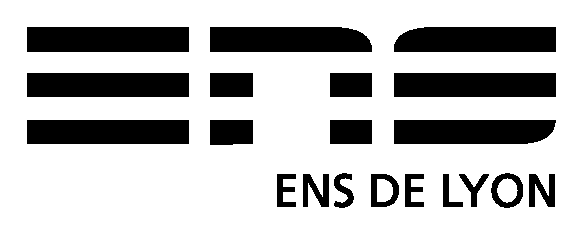
\includegraphics[height=2cm]{logoens.eps} \hfill 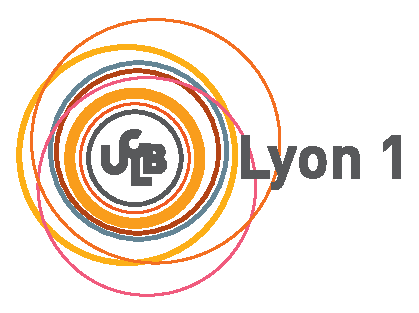
\includegraphics[height=2cm]{logoucbl.eps} \hfill 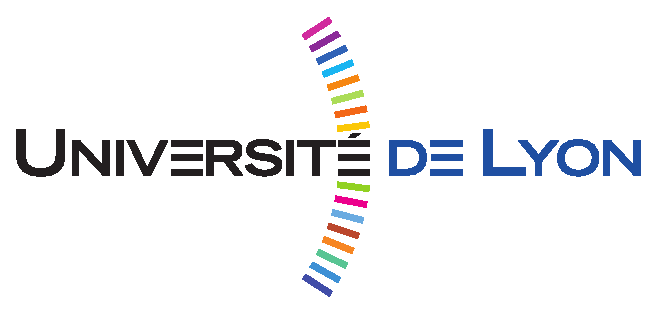
\includegraphics[height=2cm]{logounivlyon.eps}

\vspace{0.5cm}

\begin{tabularx}{\textwidth}{@{} l X l @{} }
{\sc Licence Science de la matière} 	&	& Stage 2022--2023 \\
{\it \'Ecole Normale Sup\'erieure de Lyon}		&	&  \\
{\it Universit\'e Claude Bernard Lyon I}		& 	& L3 Physique
\end{tabularx}

\begin{center}

\vspace{1.5cm}

\rule[11pt]{5cm}{0.5pt}

\textbf{\huge Génération de seconde harmonique}

\rule{5cm}{0.5pt}

\vspace{1.5cm}

\parbox{15cm}{\small
	\textbf{R\'esum\'e}: \it L'équipe de Jérôme Beugnon du groupe Gaz quantiques du Laboratoire Kastler Brossel et du Collège de France, dirigé par Jean Dalibard, manipule des gaz de Bose 2D de rubidium. Le refroidissement et le piègeage des atomes nécessite de nombreux lasers, aux longeurs d'onde adaptées aux différentes transitions atomiques que l'on cherche à exploiter.
 %Les expériences de gaz d'atomes froids utilisent des lasers pour piéger les atomes qui doivent être à des longeurs d'ondes adaptées aux différentes transitions atomiques que l'on cherche à exploiter.
	L'objectif principal de mon stage a été la conception d'un laser à $\SI{532}{\nano\metre}$ (dans le vert) par génération de fréquence double à partir d'un laser infrarouge à 1064 nm. J'ai réalisé l'intégralité du montage et fait varier les différents paramètres disponibles afin d'essayer d'optimiser la puissance et la stabilité du faisceau vert produit. On constate que, du fait des effets thermiques, il est très difficile d'obtenir une puissance stable de l'ordre de quelques watts comme espéré. 
\vspace{0.5cm}
} 


\vspace{0.5cm}

\parbox{15cm}{
\textbf{Mots clefs} : \it optique non-linéaire, génération de seconde harmonique (SHG), niobate de lithium périodiquement polé (PPLN), fibre optique, cristaux photoniques}%TODO

\vspace{0.5cm}

\parbox{15cm}{
Stage encadr\'e par :

{\bf Jérôme \textsc{Beugnon}}

\href{mailto:beugnon@lkb.ens.fr}{\tt beugnon@lkb.ens.fr} / t\'el. (+33) 1 44 27 14 31


Laboratoire Kastler Brossel

{\it Adresse

Postale}

\url{http://adresse.web.du/laboratoire/}
} 

\vspace{0.5cm}


\includegraphics[height=5cm]{./img/logos.png}

%{\tiny \it Logos du laboratoire, de l'universit\'e d'accueil,\\ de l'organisme\ldots (\'eventuellement)}
\end{center}

\vfill
\hfill \today

\end{@empty}

\newpage

\thispagestyle{empty}
\section*{Remerciements}

Je tiens à remercier toute l'équipe Gaz quantiques du Laboratoire Kastler Brossel et du Collège de France pour son accueil chaleureux et pour m'avoir fait découvrir le monde de la recherche de l'intérieur. Je remercie tout particulièrement Franco Rabec pour avoir pris le temps de m'expliquer tous les détails de l'expérience sur laquelle il travaille et Guillaume Brochier pour sa disponibilité, son aide et ses précieux conseils. Je remercie également Benjamin Huard pour m'avoir conseillé ce stage. Enfin, je remercie Jérôme Beugnon, mon maîre de stage, pour sa disponibilité, ses conseils et toutes les connaissances qu'il m'a transmises, ainsi que pour le temps qu'il m'a consacré pendant mon stage mais également en amont pour planifier mon stage et préparer tout le matériel nécessaire. 
\tableofcontents
\newpage


\setcounter{page}{1}


\setlength{\parindent}{16pt}

\section{Introduction}
%Parler du labo, omniprésence des lasers (ralentissement, piègeage, excitation)

%Objectif: lasers IR moins chers et plus robustes -> obtenir du vert par SHG

\subsection{Expériences de rubidium}

La réalisation d'expériences de physique quantique sur des gaz d'atomes nécessite de pouvoir les refroidir jusqu'à des températures en-dessous du kelvin et, souvent, de les piéger dans des potentiels contrôlés. Le refroidissement et le piégeage d'atomes neutres est réalisé avec différentes techniques, parfois combinées ou enchaînées, mais toutes reposant sur l'utilisation de lasers, ce qui explique leur importance cruciale dans ces expériences.

Dans le projet Rubidium du groupe Gaz quantiques (LKB - Collège de France), les atomes refroidis et piégés par une séquence de piège magnéto-optique (MOT), de pièges magnétique et optique et de refroidissements par évaporation, que nous ne discuterons pas ici, sont ensuite confinés dans un plan pour former un gaz dégénéré à 2 dimensions avec de l'ordre de $10^5$ atomes à \SI{20}{nK}. Comme expliqué dans la sous-section suivante, un laser vert (à \lmbd{532}) pousse les atomes de rubidium vers un minimum d'intensité. 
Ainsi, en éclairant le nuage d'atomes avec un faisceau vert (vertical sur la figure) dont le profil, réalisé avec un DMD (\textit{digital mirror device}) est en forme d'anneau, on réalise une ``boîte'' circulaire avec un puits de potentiel plat dans laquelle les atomes sont confinés. Pour geler le degré de liberté vertical, on fait interférer deux faisceaux cohérents inclinés pour réaliser une figure d'interférence constituée de franges planes, comme on peut le voir figure \ref{fig:accordeon} (les 2 faisceaux en question sont les faisceaux vert clair sur la figure), et on confine les atomes dans un des minima. Pour ce faire, on commence par piéger l'intégralité des atomes dans un même minimum d'intensité en créant une figure avec une interfrange large, puis on resserre progressivement l'interfrange en faisant varier l'inclinaison des faiceaux. En forçant une évaporation optique, on ne garde que les atomes moins énergétiques de sorte qu'à la fin de la séquence expérimentale, l'intégralité des atomes soit dans le mode fondamental du puits. Les atomes ont alors une fonction d'onde gaussienne d'épaisseur de l'ordre de \lmbd{180} \citep{brice}. On voit figure \ref{fig:accordeon} en bleu une image des atomes piégés dans le disque. Un deuxième DMD avec un nouveau laser vert peuvent alors être utilisés pour façonner différents potentiels à l'intérieur de la ``boîte''.

\begin{figure}[htbp] 
	\centering
	%
	\begin{subfigure}[b]{0.48\textwidth}
    	\centering
    	\small
	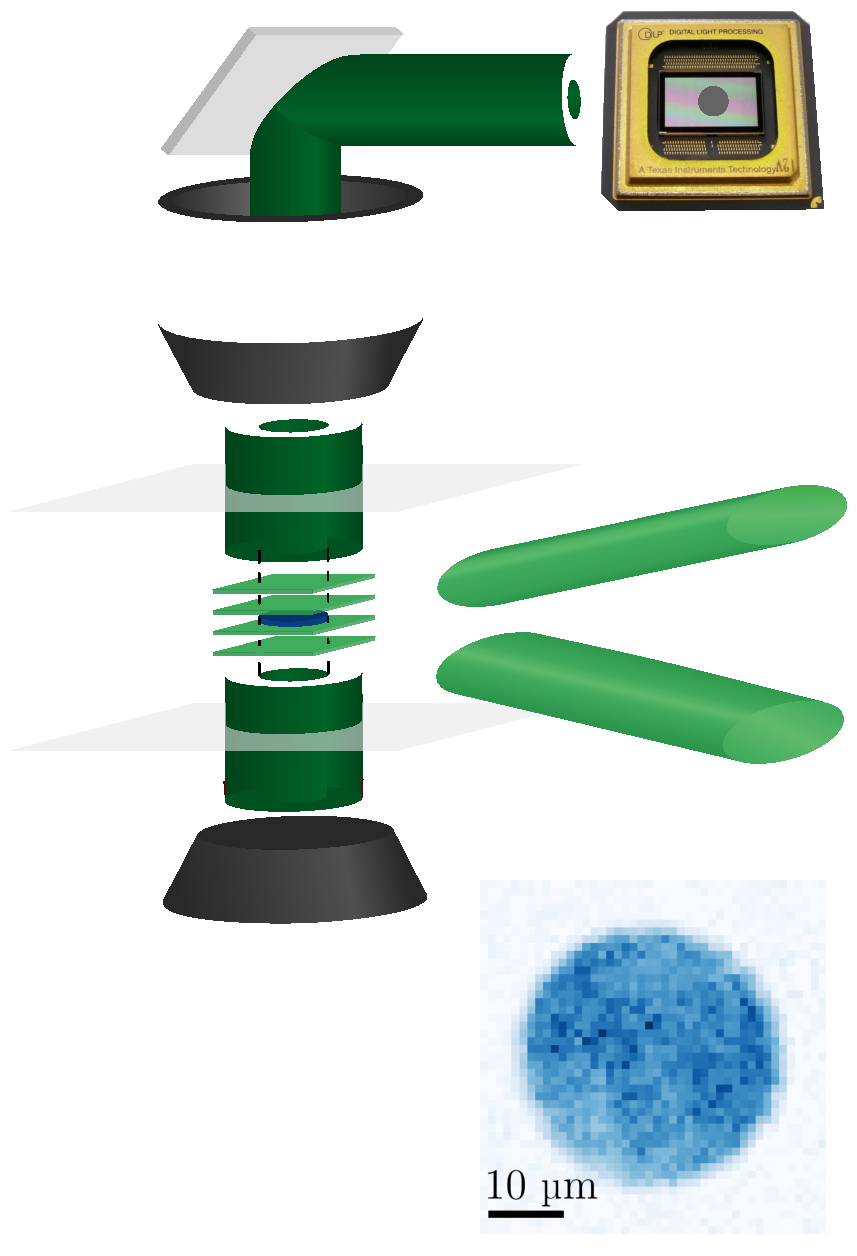
\includegraphics[height=9cm]{img/accordeon-dmd.pdf}
	\caption{\small Réalisation d'un piège circulaire 2D \ncite{ville}} %\footnotemark}
		\label{fig:accordeon}
	\end{subfigure}	
	%
	\begin{subfigure}[b]{0.48\textwidth}
		\centering
		\small
		\resizebox{!}{9cm}{
   			\begin{tikzpicture}[
level/.style = {
        ultra thick,
        red,
    },
    laser/.style = {
        ultra thick,
        green,
        dashed
    },
    connect/.style = {
        dashed,
        red
    },
    trans/.style={thick,->,shorten >=2pt,shorten <=2pt,>=stealth},
    notice/.style = {
        draw,
        rectangle callout,
        callout relative pointer={#1}
    },
    label/.style = {
        text width=2cm
    }
]
    % Draw all levels
    \draw[level] (0,0) --  +(-2,0) node[left] {$3S^{1/2}$} ;
    \draw[level] (0,4) --  +(-2,0) node[left] {$3P^{1/2}$} ;
    \draw[level] (0,4.5) --  +(-2,0) node[left] {$3P^{3/2}$};
    \draw[laser] (0,6) --  +(-2,0) node[left] {laser};
    
    \draw[trans] (-1.1,0) -- +(0,4) node[pos=0.4,left] {794.8 nm}; %794.8
    \draw[trans] (-1,0) -- +(0,4.5) node[pos=0.6,left] {780.0 nm}; %780.0
    \draw[trans] (-0.5,0) -- +(0,6) node[pos=0.85,left] {532 nm};
    
\end{tikzpicture}

		}
		\caption{\small Transitions du rubidium 87}
		\label{fig:transitions}
	\end{subfigure}
	%

	\caption{Utilisation du laser à \lmbd{532} dans l'expérience : \small le laser est à une fréquence très supérieure à celle des transitions du rubidium 87, ce qui permet de piéger les atomes dans les minima d'intensité}
\end{figure}

%\footnotetext{schéma extrait de la thèse de Brice Bakkali-Hassani, ancien doctorant sur l'expérience}


\subsection{Utilisation des lasers à 532 nm}

Alors que le refroidissement des atomes se fait avec des lasers résonants, c'est-à-dire de fréquence proche de celle de la transition visée, et repose sur l'échange d'impulsion lors de l'absorption et la réémission de photons, le piégeage est réalisé avec des lasers non-résonants, désaccordés soit vers le rouge (\textit{i.e.} de fréquence très inférieure à celle des transitions atomiques), soit vers le bleu (\textit{i.e.} de fréquence très supérieure à celle des transitions atomiques), et repose sur le principe du piégeage optique dipolaire exploitant l'interaction champ électrique - dipôle électrique induit.

C'est le cas des lasers à \lmbd{532}, qui sont désaccordés vers le bleu pour le rubidium 87 comme on peut le voir sur le diagramme des transitions figure \ref{fig:transitions}.

Cette interaction donne lieu, classiquement, à une force dérivant du potentiel $U_\mathsc{dip}(\v r) = {-\frac12 \langle \v d \cdot \v E \rangle} = -\frac{1}{2\varepsilon_0 c}\mathfrak{Re}\left(\alpha(\omega)\right) I(\v r)$ ($\v d$ désigne le moment dipolaire induit, $\alpha$ la polarisabilité complexe, $\langle \cdot \rangle$ une moyenne temporelle et $I$ l'intensité du faisceau)
%\footnote{Le facteur $\frac12$ est dû au fait que le dipôle est non pas permannent mais proportionnel au champ appliqué.} %En effet, pour $\v d = \alpha \v E$, $\v F = (\v d \cdot \v \nabla) \v E = \frac12 \v \nabla (\v d \cdot \v E)$}  %
qui va servir à piéger les atomes dans un minimum de potentiel. Le rayonnement laser va également engendrer des cycles d'absorption et réémission spontanée, ayant lieu, toujours ``classiquement'', à une fréquence $\Gamma_\mathsc{diff} = \frac{P_\mathsc{abs}}{\hbar \omega} = \frac{1}{\hbar \varepsilon_0 c} \mathfrak{Im}\left(\alpha(\omega)\right) I(\v r)$ où $P_\mathsc{abs} = \langle \dot{\v d} \cdot \v E \rangle$ est la puissance absorbée par l'atome, qui vont conduire à un réchauffement des atomes. 
Pour un atome à deux niveaux avec une transition à $\omega_0$, dans l'approximation de faible saturation (état excité faiblement peuplé) et de fort désaccord ($\Delta = \omega - \omega_0$ vérifiant $|\Delta| \ll \omega_0$), vérifiée en pratique et permettant de justifier le calcul classique (à une précision de l'ordre du pourcent), on trouve
\vspace{-0.2cm}
\begin{align}
	U_\mathsc{dip}(\v r)&=\frac{3\pi c^2}{2\omega_0^3} \frac{\Gamma}{\Delta} I(\v r) \\
	\Gamma_\mathsc{diff}(\v r)&=\frac{3\pi c^2}{2\hbar\omega_0^3} \left(\frac{\Gamma}{\Delta}\right)^2 I(\v r) 
\end{align}

avec $\Gamma = \frac{\e 2 \omega^2}{6 \pi \varepsilon_0 m_e c^3}$ la largeur naturelle de la transition, qui correspond dans une vision classique au facteur d'amortissement dû au rayonnement.

Puisque $\Gamma_\mathsc{diff}=\frac{\Gamma}{\hbar \Delta} U_\mathsc{dip}$, on voit qu'un grand désaccord permet de minimiser le chauffage dû à la diffusion. On remarque également que pour un faisceau laser désaccordé vers le rouge, l'atome est piégé dans les zones lumineuses, alors que pour un désaccord vers le bleu, l'atome est piégé dans les zones sombres.

Pour un atome réel à plusieurs niveaux, l'énergie d'interaction (qui s'obtient plus rigoureusement en considérant la perturbation par un hamiltonien de couplage $\mathcal H_1 = - \hat{\v d} \cdot \v E$ des états propres du système atome + champ) est la somme des contributions des différents états excités, pondérée par l'importance des transitions associées \citep{grimm}. Pour les atomes de rubidium 87 utilisés dans l'expérience, les transitions prépondérantes sont les 2 transitions de la ligne D qui sont représentées figure \ref{fig:transitions}.


\subsection{Objectif du stage}

Les lasers verts actuellement utilisés au laboratoire sont des lasers à \lmbd{1064} Nd-Yag ``solides'' ou des lasers à fibres qui sont vendus directement avec le doublage de fréquence. Ils ont l'inconvénient d'être particulièrement onéreux et fragiles, et leur réparation nécessite plusieurs mois d'attente. L'objectif de mon projet était donc d'explorer la possibilité de réaliser le doublage soi-même à partir d'un laser à \lmbd{1064} beaucoup plus facile d'accès. Ce doublage de fréquence (SHG pour \textit{second harmonic generation} en anglais) repose sur l'existence d'un terme dans la polarisation électrique de certains cristaux quadratique en le champ appliqué, qui joue le rôle d'un terme source à la fréquence double de celle du faisceau incident. C'est notamment le cas du niobate de lithium choisi pour ce projet. %Le principe sera expliqué plus en détail section \ref{SHG}. 

\section{Couplage de la fibre à cristaux photoniques}
Une première partie de mon stage, indépendante de l'objectif principal d'obtenir un laser vert, a été de tester une fibre à cristaux photoniques
%, plus précisément une fibre de verre à trous (\textit{holey fiber}) 
LMA-PM-10 de la marque NKT Photonics. LMA signifie large (effective) mode area et donc que la fibre est faite pour des faisceaux larges, ce qui est important pour les applications avec des lasers de plusieurs dizaines de watts, car le seuil de destruction des matériaux ainsi que les effets thermiques dus à la dissipation dépendent de l'intensité et non de la puissance totale. La fibre utilisée a un mode de $\SI{8.6}{\micro\meter}$ de diamètre alors que les fibres traditionnelles ont plutôt un diamètre de $\SI{3}{\micro\meter}$. L'utilisation d'une fibre à cristaux photoniques LMA permet donc de réduire l'intensité de presque un ordre de grandeur.

La technologie des fibres optiques traditionnelles, reposant sur une réflexion interne totale, ne permet pas de fabriquer des fibres à c\oe ur large qui resteraient monomodes sur une gamme de longueurs d'ondes et de rayon de courbure de la fibre suffisante. 
Les fibres à cristaux photoniques, quant à elles, reposent sur une variation d'indice optique effectif périodique grâce à une structure régulière de trous et ont l'avantage de permettre beaucoup plus de liberté, notamment en terme de taille du c\oe ur tout en restant monomodes, et ce sur une très large gamme de fréquences.  
%Cette structure conduit à des bandes interdites analogues à celles des électrons dans un crystal (ondes de Bloch). 
\citep{russell2006,russell2007}

%Contrairement aux fibres traditionnelles, la variation d'indice optique dans ces fibres est réalisée à l'aide d'une structure régulière de trous. En effet, l'air aillant un indice optique inférieur au matériau de la fibre, les trous permettent de réduire l'indice moyen. % TODO: corriger

\begin{figure}[htpb]  
\centering
\hspace*{0.4cm}
\begin{subfigure}[t]{0.38\textwidth}
	\centering
	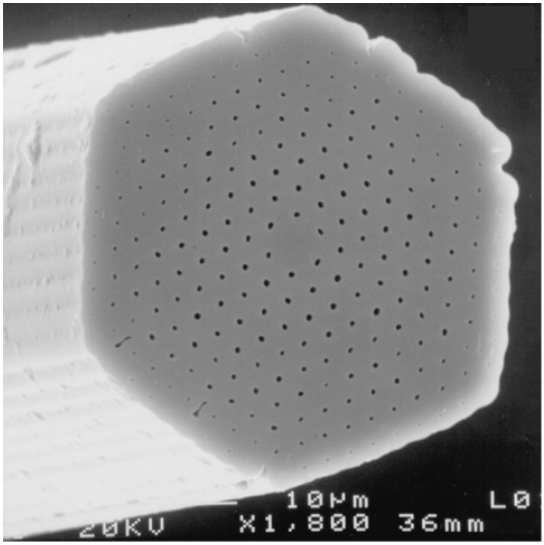
\includegraphics[height=5.3cm]{../biblio/solid core PCF - russell2006}
	\caption{Image par microscopie électronique par balayage de la première fibre à cristaux photoniques fonctionnelle \ncite{russell2006}}
	\label{fig:PCF}
\end{subfigure}
\hspace*{0.4cm}
\begin{subfigure}[t]{0.37\textwidth}
	\centering
	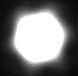
\includegraphics[height=5.3cm]{./img/mode hexa.png}
	\caption{Image en intensité du mode hexagonal en sortie (caméra fortement saturée)}
	\label{fig:hexa}
\end{subfigure}
\hspace*{-0.8cm}
\caption{Structure de la fibre à cristaux photoniques et mode hexanogal en sortie}
\end{figure}

Comme indiqué, la fibre à cristaux photoniques ne sélectionne qu'un seul mode. Les fibres monomodes traditionnelles sélectionnent généralement un mode gaussien, mais la géométrie de la fibre à cristaux photoniques utilisée fait que le mode sélectionné est un mode hexagonal, comme on peut le voir figure \ref{fig:hexa}. Ce mode ne se distingue cependant que très peu d'un mode gaussien, et on ne voit la forme hexagonale qu'en saturant la caméra.

En particulier, afin de maximiser la transmission de la fibre, il faut que l'axe de propagation du faisceau incident (gaussien) coïncide avec celui de la fibre, ce qui correspond à l'ajustement de 4 paramètres (2 angles pour l'orientations et 2 coordonnées pour la position dans le plan transverse). L'ajustement est fait à l'aide de 2 miroirs (cf schéma figure \ref{fig:couplage}). Il faut également que le faisceau ait le bon waist et qu'il soit focalisé en bout de fibre. La focalisation est réalisée à l'aide d'un coupleur de fibre (60SMS-SMA-0-M5-08 de la marque Schäfter+Kirchhoff), qui est un collimateur de focale 5 mm optimisé pour le couplage de fibres et nécessite de produire un faisceau collimaté en amont du coupleur avec le bon waist (que l'on peut déterminer expérimentalement en observant le faisceau en sortie de fibre, puisqu'elle est équipée d'un coupleur identique). Cet ajustement est fait à l'aide d'un téléscope avec des focales adaptées.

\begin{figure}[h]
	\centering
	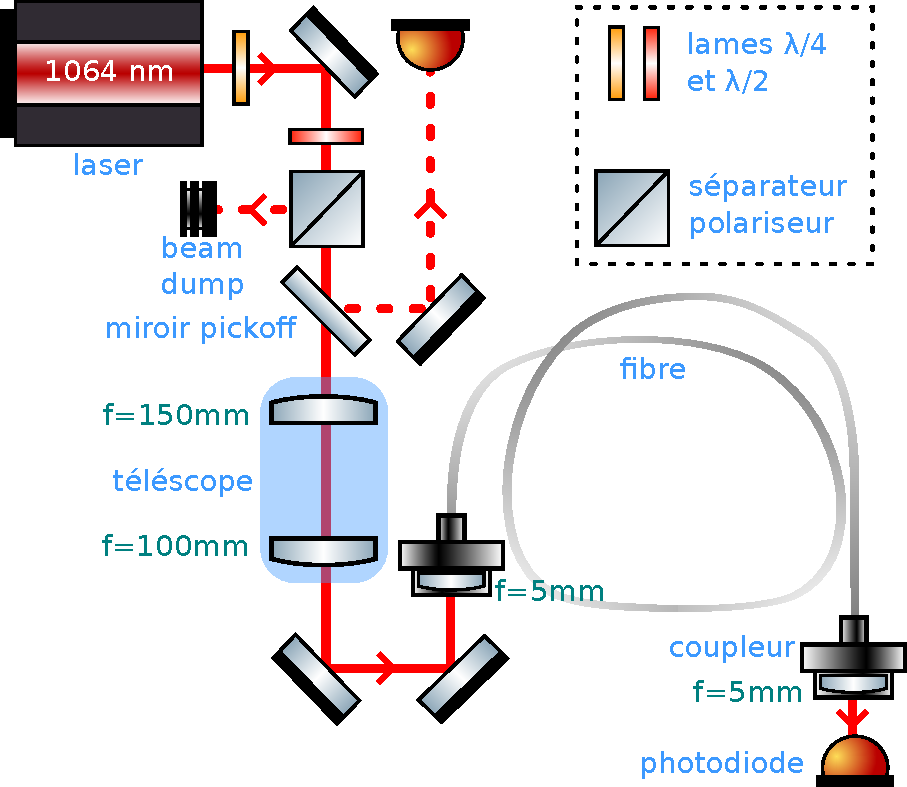
\includegraphics[width=0.7\textwidth]{./img/schema couplage.pdf}
	\caption[Montage de la fibre à cristaux photoniques]{Montage de la fibre à cristaux photoniques :
	\small Le cube séparateur permet de sélectionner une polarisation linéaire, et les lames d'onde servent à maximiser la composante du champ selon la direction transmise afin de minimiser les pertes. La composante réfléchie finit dans un ``beam dump'', fait pour absorber le rayonnement infrarouge et dissiper la chaleur. Le ``pickoff'', lame de verre avec un traitement adapté, sert à réfléchir une petite partie du faisceau pour l'envoyer sur une photodiode. Une calibration permet de corréler la tension sur la photodiode à la puissance en sortie du séparateur. Le téléscope, de grandissement $\gamma = \frac{100}{150} = 0.67$, sert à produire un faisceau collimaté avec le waist souhaité, et enfin le coupleur d'entrée de fibre sert à adapter le faisceau incident à la fibre. Le coupleur de sortie sert à obtenir un faisceau collimaté et plus large qu'au sein de la fibre. Une deuxième photodiode permet de mesurer la puissance transmise et évaluer l'efficactié du couplage.}
	\label{fig:couplage}
\end{figure}

De façon plus détaillée, le protocole du couplage est essentiellement le suivant :
\begin{enumerate}
	\item On choisit une hauteur de faisceau avec laquelle on va trailler, et on aligne la source laser et les optiques à cette hauteur.
	\item À l'aide des vis des 2 miroirs réglant l'angle vertical, on assure l'horizontalité et la bonne hauteur du faisceau par rapport au collimateur en faisant passer le faisceau à travers ce dernier.
	\item On connecte la fibre au collimateur. Si l'alignement est bon, on doit avoir une puissance mesurable en sortie.
	\item Pour déterminer le waist adapté à la fibre et au coupleur, on utilise la présence d'un coupleur identique à l'autre extrémité de la fibre. En effet, le faisceau gaussien en sortie aura, par retour inverse de la lumière, le bon waist à injecter dans la fibre. Le waist du mode en sortie est déterminé par la mesure à la caméra du diamètre du faisceau à différentes positions.	
	\item On monte un téléscope avec un grandissement permettant d'obtenir le waist voulu.
	\item On alterne optimisation de la position du collimateur et de l'alignement. Il faut se méfier que le déplacement du collimateur affecte l'alignement.
	\item L'alignement s'effectue selon la méthode du `beam-walk' : les rotations des 2 miroirs selon le même axe ont un effet couplé, permettant par exemple d'induire une translation pure du faisceau. Il est donc préférable de faire varier un angle et trouver le maximum pour cet angle en faisant varier l'angle associé sur le deuxième, et comparer ces maxima successifs. En effet, le couplage est sensible même aux petites variations d'angle, mais les maxima successifs obtenus en `beam-walkant' sont assez proches. 
\end{enumerate}

J'ai ainsi pu obtenir un couplage d'environ $\SI{75}{\percent}$, ce qui est tout à fait raisonnable. En particulier, on peut injecter $\SI{10}{W}$ dans la fibre sans risquer de l'endommager du fait d'une trop forte dissipation de puissance.

TODO: injection en pola


\section{Principe de la génération de seconde harmonique ( SHG)} %\'Etude th\'eoriqaue de la génération de seconde harmonique (SHG)}
\label{SHG}

Nous revenons maintenant à l'objectif principal du stage, l'obtention d'un laser à \lmbd{532} par génération de seconde harmonique, dont nous expliquons d'abord le principe.

\subsection{Polarisation non linéaire et seconde harmonique} 

\begin{figure}[h]
\centering
\begin{subfigure}{0.45\textwidth}
	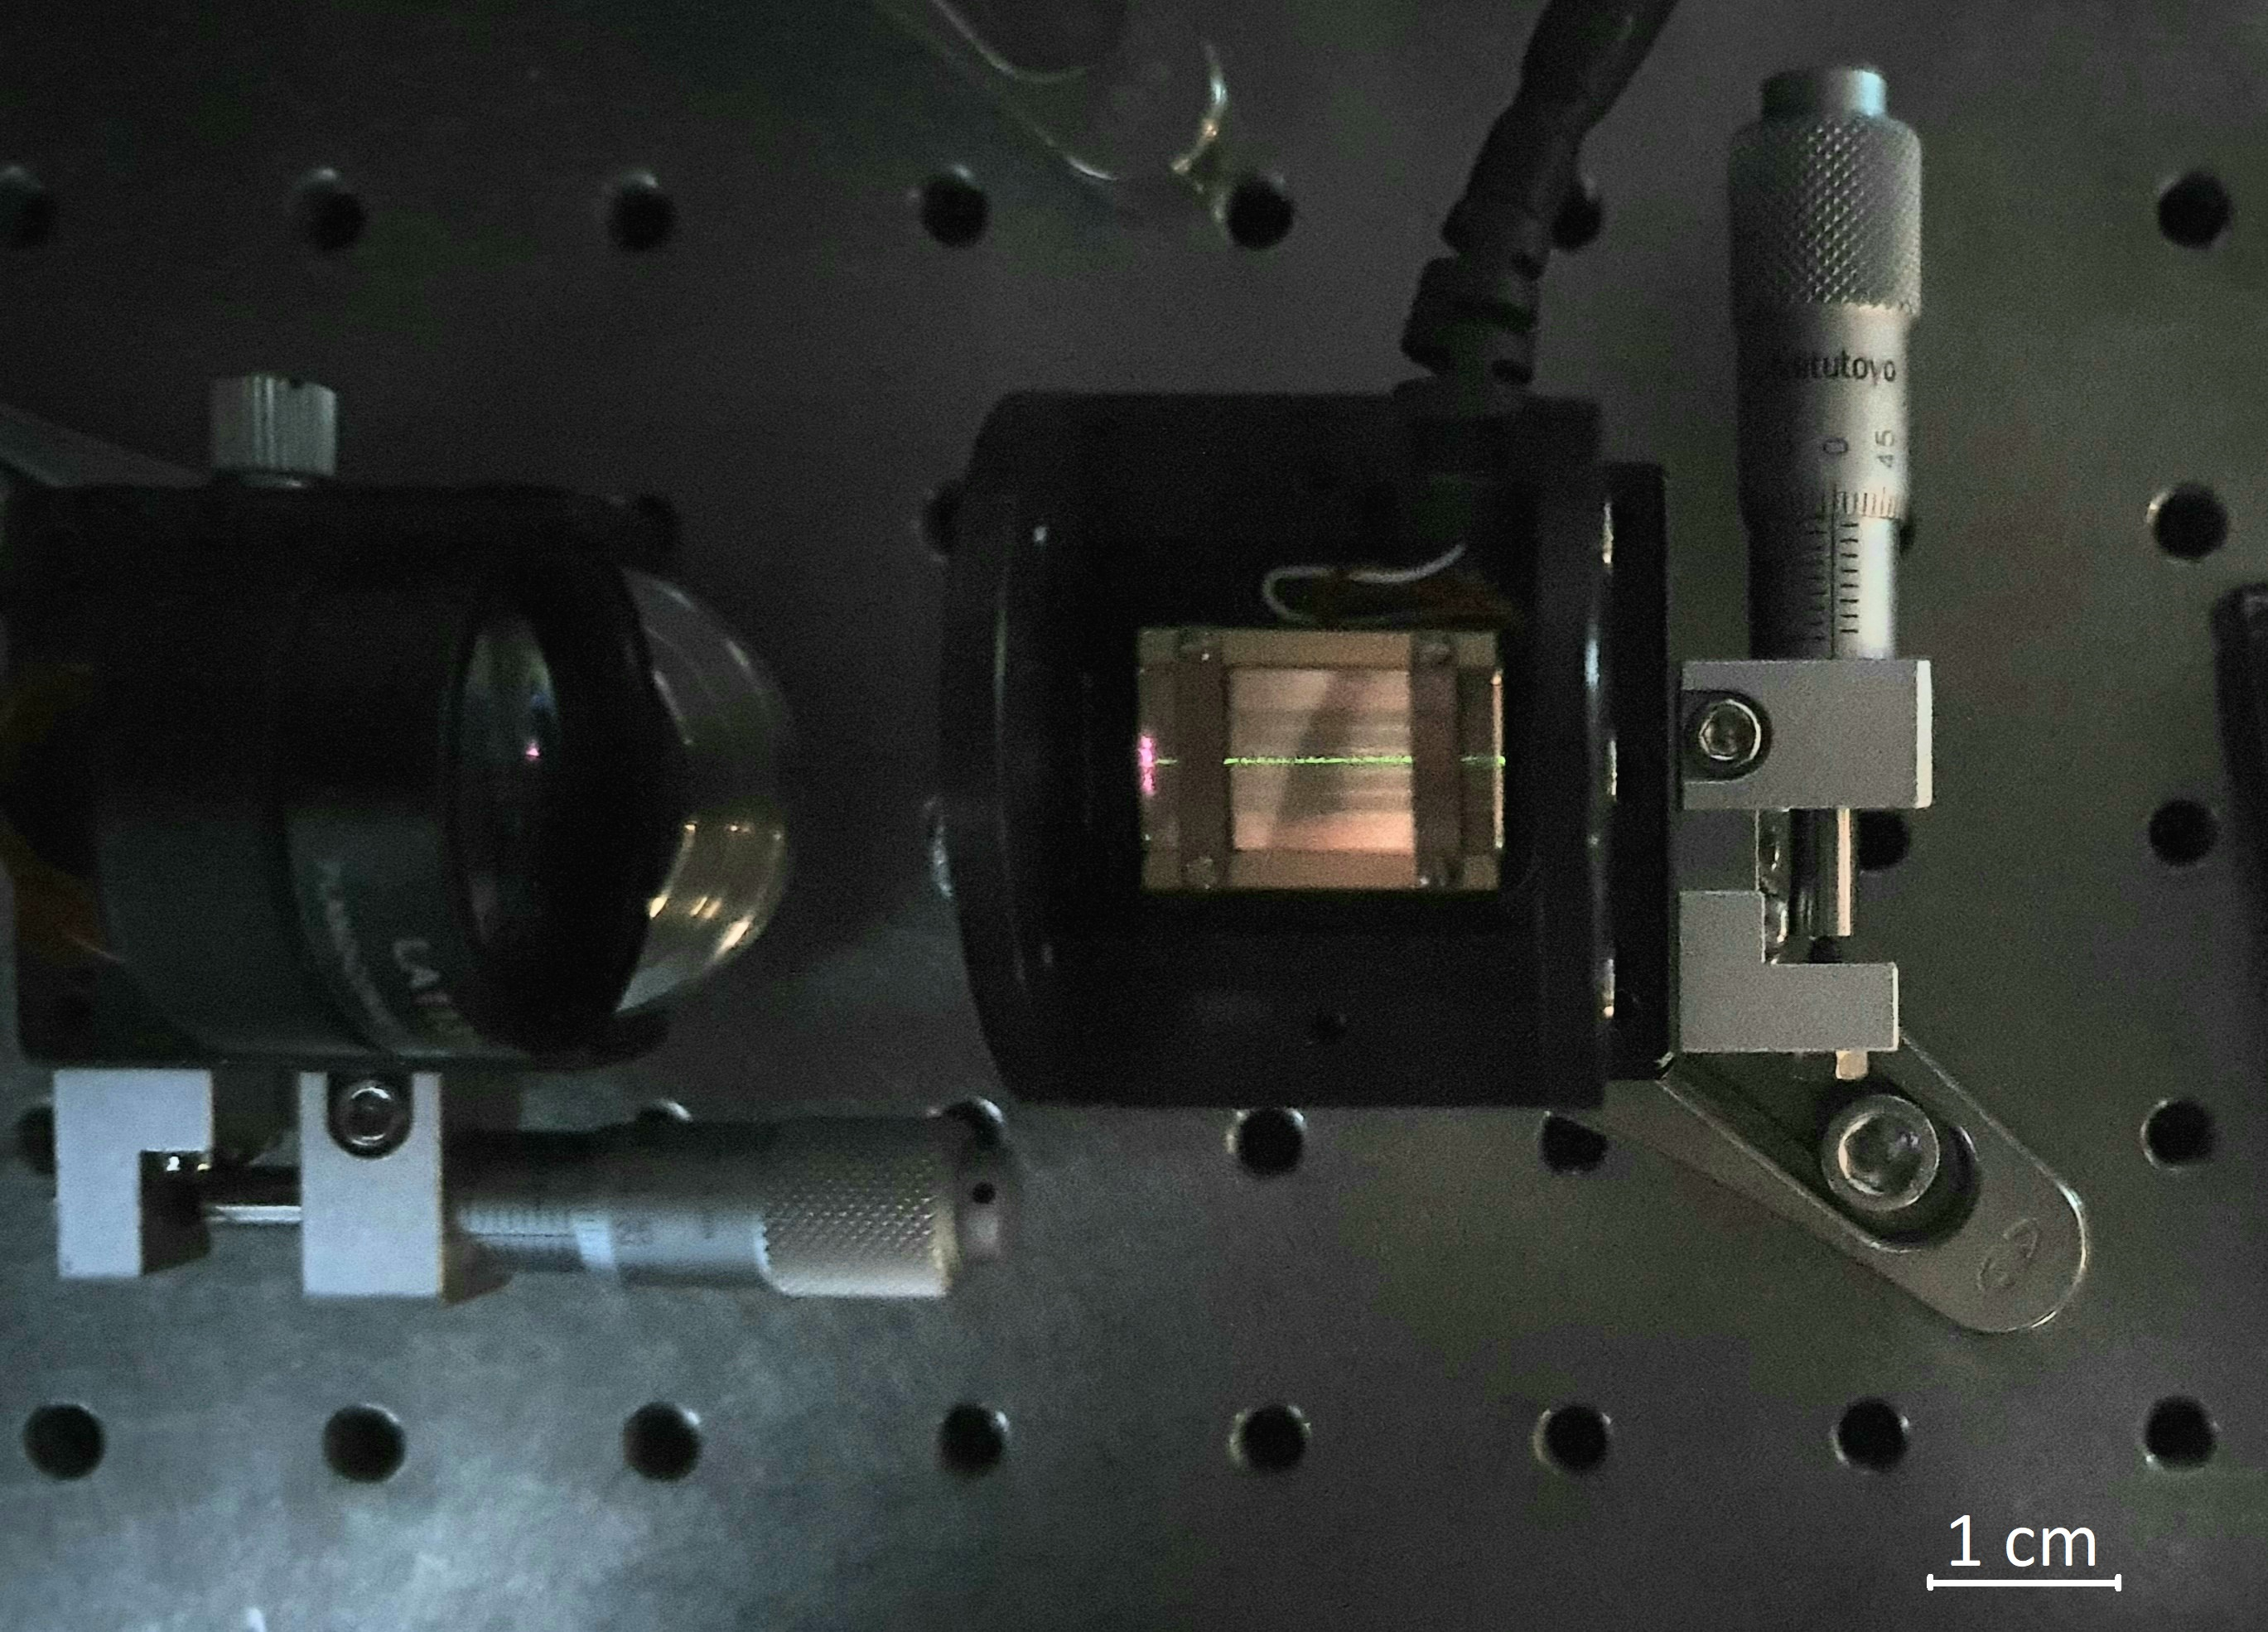
\includegraphics[width=\textwidth]{./img/cristal clair.jpg}
\end{subfigure}
\begin{subfigure}{0.5\textwidth}
	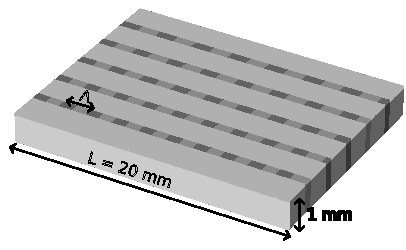
\includegraphics[width=\textwidth]{./img/cristal.pdf}
\end{subfigure}
\caption{Génération d'un laser vert dans un cristal doubleur de fréquence : \small le faisceau incident passant par une des bandes avec une structure de période $\Lambda$, dont le rôle est expliqué section \ref{qpm}, donne lieu à un faisceau vert grâce à la polarisation d'ordre 2 du cristal}
\label{fig:cristal}
\end{figure}

La génération de la seconde harmonique a lieu dans un cristal doubleur de fréquence avec des propriétés non-linéaires favorables (figure \ref{fig:cristal}).
La propagation d'ondes électromagnétiques dans un milieu non linéaire non magnétique donne lieu à une équation d'onde avec un terme source, qui s'écrit 
\begin{align}
\boldsymbol{\nabla}^2 \boldsymbol{\E}_q + \frac{\omega_q^2}{c^2}\tens\epsilon^{(1)}(\omega_q)\cdot \v \E_q(\v r) = - \frac{\omega_q^2}{\epsilon_0 c^2} \boldsymbol{\mathcal{P}}^\mathsc{NL}_q(\v r)
\end{align}
dans le domaine de Fourier en temps avec la convention $\v E(\v r, t) = \mathfrak{Re} \left\{ \sum_{q \in \mathbb N} \v {\boldsymbol{\mathcal E}}_q (\v r) \e{-i \omega_q t} \right\}$ et $\v P^\mathsc{NL} (\v r, t) = \mathfrak{Re} \left\{ \sum_{q \in \mathbb N} \v {\boldsymbol{\mathcal P}}^\mathsc{NL}_q (\v r) \e{-i \omega_q t} \right\}
$,
%, avec n un indice désignant la composante spectrale (il s'agira dans notre cas de l'ordre de l'harmonique), 
avec $\tens \epsilon^{(1)}$ le tenseur de permittivité diélectrique relative associé à la partie linéaire de la polarisation et $\v P^\mathsc{NL}_q$ la partie non-linéaire de la polarisation (cf annexe \ref{NL}) \ncite{boyd,joffre}.

On fait l'hypothèse simplificatrice d'une \textbf{polarisation linéaire} selon un des axes principaux et on travaillera par la suite avec des $\mathcal E_q$ scalaires. En particulier, la permittivité tensorielle $\tens \varepsilon^{(1)}$ est remplacée par sa valeur propre correspondante et donne lieu à un indice optique $\boxed{ n_q = \sqrt{ \varepsilon^{(1)}(\omega_q)}}$. En écrivant les différentes harmoniques sous la forme d'une ``onde monochromatique d'amplitude variable'' $\mathcal E_q = \A_q(x,y,z) \e{ik_qz}$ avec $\boxed{k_q =\frac{n_q \omega_q}{c}}$ et en se plaçant dans l'approximation paraxiale, i.e. de lente variation de $\A$ avec $z$ $\left(\frac{\partial^2 \A_q}{\partial z^2} \ll k_q \frac{\partial \A_q}{\partial z}\right)$, on arrive aux équations \ncite{joffre}
\begin{align}  
	\left\{\v\nabla_\bot + 2 i k_q \frac{\partial}{\partial z} \right\} \A_q = - \frac{\omega_q^2}{\varepsilon_0 c^2} \v P^\mathsc{NL}_q (\v r) \e{-ik_qz}
	\label{eq:parax}
\end{align}
avec $\v\nabla_\bot = \pdv{}{x^2} + \pdv{}{y^2}$.

En particulier, pour un champ électrique avec une composante à $\omega$ et une à $2\omega$, le terme quadratique dans la polarisation est donné par \ncite{joffre}
\begin{equation}
\begin{aligned}
	P^{(2)} &= \varepsilon_0 \chi^{(2)} \v E^2  \text{ avec $\chi^{(2)}$ la susceptibilité d'odre 2}\\
	&= \frac{\varepsilon_0 \chi^{(2)}}{4} \left\{\mathcal E_1 e^{-i\omega t} + \mathcal E_1^* e^{i\omega t} + \mathcal E_2 e^{-2i\omega t} + \mathcal E_2^* e^{2i\omega t} \vphantom{\frac12}\right\}^2 \\
	&= \frac{\varepsilon_0 \chi^{(2)}}{4} \left\{\mathcal E_1^2 \e{-2i\omega t} + \E_1^{*2} \e{2i\omega t} + 2|\mathcal E_1|^2 + 2 \E_1\E_2^* \e{i\omega t} + 2 \E_1^*\E_2 \e{-i\omega t} \vphantom{\frac12}\right. \\
	&\qquad\qquad\qquad \left. + 2 \E_1\E_2 \e{-3 i\omega t}  + 2 \E_1^*\E_2^* \e{3 i\omega t} + \mathcal O(\E_2^2) \vphantom{\frac12}\right\} \\ 
%	&= \mathfrak{Re} \left\{ \sum_{q \in \mathbb N} \v {\boldsymbol{\mathcal P}}^{(2)}_q \e{-i \omega_q t} \right\}
\end{aligned}
\end{equation}
où l'on a considéré que $\chi^{(2)}$ est approximativement le même pour toutes les harmoniques. 
% où l'on a considéré que $\chi^{(2)}$ est le même pour toutes les harmoniqes pour un milieu supposé sans pertes \ncite{boyd}.

On voit donc que l'onde incidente (à $\omega$) conduit à un terme à la fréquence double dans la polarisation, qui va conduire à la création d'une onde à cette seconde harmonique comme souhaité. Cette dernière va conduire à un terme à la fréquence fondamentale qui va affecter l'onde incidente ainsi qu'à un terme à la fréquence triple qui va conduire à une onde à la troisième harmonique et ainsi de suite. 
Dans l'hypothèse où la seconde harmonique est d'amplitude faible par rapport au faisceau incident, nous pouvons cependant négliger ces termes d'ordre supérieur. Cette hypothèse, connue sous le nom \textbf{d'hypothèse de non-déplétion}, est discutée en annexe \ref{ndepl}. Nous négligerons également le terme constant dit de redressement. %Nous nous plaçons cependant dans l'hypothèse que la seconde harmonique 

%En écrivant les différents champs 

%Plus précisément, en écrivant les équations d'onde paraxiales pour les différentes harmoniques, 

Ceci conduit à l'équation d'évolution de l'amplitude de l'onde générée $\A_2$ suivante:
\begin{align}
	\left\{\v\nabla_\bot + 2 i k_2 \frac{\partial}{\partial z} \right\} \A_2 = - \frac{2 \chi^{(2)} \omega^2}{c^2} \A_1^2 \e{- i (k_2 - 2k_1) z}
	\label{eq:SHG}
\end{align}

\subsection{Le problème de l'accord de phase}
\label{qpm}
Cette équation est beaucoup plus abordable dans l'approximation d'une onde plane avec $\A_1$ et $\A_2$ ne dépendant que de $z$ (et donc $\A_1$ constante dans \textbf{l'hypothèse de non-déplétion}):
\begin{align}
	\dv{\A_2}{z} &= i\frac{\chi^{(2)}\omega}{2cn_2} \A_1^2 \e{-i \Delta k z} \text{ avec } \boxed{\Delta k = k_2 - 2k_1} \label{eq:pwe} \\
	\text{soit } \A_2(L) &= i \frac{\chi^{(2)}\omega}{2 cn_2} \A_1^2 L \operatorname{sinc}\left( \frac{\Delta k L}{2} \right) \e{-i\frac{\Delta k L}{2}}
\end{align}
en sortie du cristal en $z=L$ avec $\A_2(0)=0$ à l'entrée.

Cette équation se comprend très bien en considérant que le carré de l'onde incidente, de nombre d'onde $2k_1$, génère un rayonnement qui se déplace ensuite à $k_2$, de sorte qu'en un point $z$ une onde de phase $2k_1z$ vient s'ajouter à une onde se propageant avec un nombre d'onde $k_2$. Ainsi, l'onde à la seconde harmonique générée en $z$ aura à la sortie du cristal en $z=L$ la phase $2k_1 z + k_2 (L-z) = k_2 L - \Delta k z$ (modulo une constante universelle), de sorte que les ondes générées en $z$ et en $z+L_\mathsc{coh} := z + \frac{\pi}{\Delta k}$ interfèrent destructivement, ce qui conduit à une amplitude nulle en sortie, comme illustré figure \ref{fig:agen}.

\begin{figure}[htpb] 
\centering
\begin{subfigure}[b]{0.48\textwidth}
	\centering
	\hspace*{-0.8cm}
	%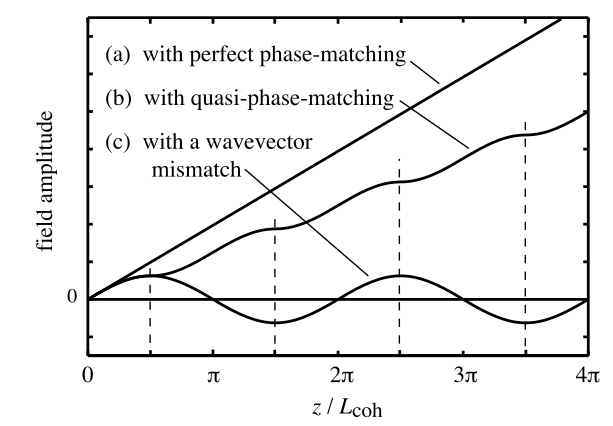
\includegraphics[height=5cm]{./img/QPM.png}
	\include{./img/qpm.tex}
	\vspace*{-1cm}
	\caption{}
	\label{fig:agen}
\end{subfigure}
\begin{subfigure}[b]{0.48\textwidth}
	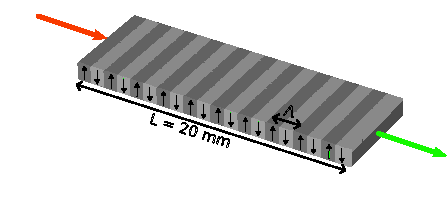
\includegraphics[height=4cm]{./img/PP.pdf}
	\vspace*{0.8cm}
	\caption{}
	\label{fig:inversion}
\end{subfigure}
\hspace*{-0.6cm}
\caption{Amplitude de seconde harmonique et quasi-accord de phase : (a) \small  Sans accord de phase, l'amplitude de la seconde harmonique retombe à zéro toutes les $2L_\mathsc{coh}$ et la croissance linéaire avec la longueur du cristal est perdue. La technique du quasi-accord de phase permet de la retrouver, bien qu'avec un coefficient plus faible. (b) L'inversion de polarisation tous les $\Lambda/2$ permet la réalisation du quasi-accord de phase.} %TODO
\label{fig:QPM}
\end{figure}

Avec le cristal de niobate de lithium utilisé, $L_\mathsc{coh}$ vaut à peine $\SI{3}{\micro\meter}$ alors que le cristal fait $\SI{2}{cm}$.
Afin d'avoir une génération efficace, il faudrait donc $\Delta k = \frac{2\pi}{\lambda_2}(n_2-n_1) = 0$ (condition d'accord de phase) avec $\lambda_2=$\lmbd{532} la longueur d'onde dans le vide de la seconde harmonqiue, soit $n_2 = n_1$. Cela n'est \textit{a priori} pas possible sans dispersion anormale. Une solution consiste alors à exploiter la biréfringence du cristal, mais cette méthode est difficile à réaliser et le $\chi^{(2)}$ correspondant à la polarisation requise est souvent assez faible. 

Nous avons choisi une autre solution qui consiste à fabriquer un cristal dont le $\chi^{(2)}$ varie spatialement. En effet, si $\chi^{(2)}(z) = \chi^{(2)}_0 \e{i k_\chi z}$, cela revient à remplacer $\Delta k$ par $\boxed{ \Delta k_\mathsc{eff} = \Delta k - k_\chi }$ dans (\ref{eq:pwe}). 
%En pratique, il est difficile de fabriquer un tel cristal, et on préfère inverser le signe de $\chi^{(2)}$ en inversant l'axe extraordinaire d'un matériau ferroélectrique avec une période $\Lambda$ (cf figure \ref{fig:QPM}). 
Évidemment, la susceptibilité est en réalité proche d'une valeur réelle et un tel $\chi^{(2)}$ n'est pas réalisable. À la place, on inverse le signe de $\chi^{(2)}$ en inversant l'axe extraordinaire d'un matériau ferroélectrique avec une période $\Lambda$ (cf figure \ref{fig:inversion}) \footnote{En effet, si $P_z = \chi^{(2)} E_z^2$ et on change $P_z$ et $E_z$ de signe, on voit que $\chi^{(2)}$ est changé en son opposé.}.
On parle alors de quasi-accord de phase et un tel cristal est dit périodiquement pôlé. Dans ce cas, la décomposition de Fourier de $\chi^{(2)}(z) = \chi^{(2)}_0 \operatorname{sgn}[\cos(2\pi z/ \Lambda)]$ montre que le terme de plus grande amplitude est le fondamental d'amplitude $\boxed{ \chi_\mathsc{eff} = \frac2\pi \chi^{(2)}_0 }$ et de nombre d'onde $\boxed{ k_\chi = \frac{2\pi}{\Lambda} }$. 
Si $k_\chi = \Delta k$, $\Delta k_\mathsc{eff} = 0$ et le terme source correspondant sera accordé en phase sur toute la longueur du cristal et permettra donc de générer la seconde harmonique. Par la suite, on ne tiendra compte que de ce terme, oubliant les autres harmoniques de $\chi^{(2)}(z)$ (cela correspond à la ligne en pointillés, qui approxime bien la courbe orange).
Ceci nous conduit à une amplitude 
\begin{align}
	\A_2(L) &= i \frac{\chi_\mathsc{eff}\omega}{2 cn_2} \A_1^2 L \operatorname{sinc}\left( \frac{\Delta k_\mathsc{eff} L}{2} \right) 
	\e{-i\frac{\Delta k_\mathsc{eff} L}{2}} \\	
	&= i \frac{\chi_\mathsc{eff} \omega}{2 cn_2} \A_1^2L 
\end{align}
si le quasi-accord de phase est respecté.

Ainsi, l'intensité de la seconde harmonique est quadratique en l'intensité du fondamental avec
\begin{align}
	\frac{\mathcal I_2}{\mathcal I_1^2} &= \frac{\frac12 n_2 \varepsilon_0 c |\A_2|^2}{\left(\frac12 n_1 \varepsilon_0 c |\A_1|^2\right)^2} 
	= \frac{\chi_\mathsc{eff}^2\omega^2}{2 n_2 n_1^2 \varepsilon_0 c^3} L^2
	\label{eq:plane}
\end{align}
%pour des faisceaux gaussiens de waists $w_0$ pour le fondamental et $\frac{w_0}{\sqrt2}$ pour la seconde harmonique que l'on va être amenés à considérer par la suite.


On notera en particulier la dépendance quadratique en la longueur du cristal \footnote{Rappelons tout de même que nous nous sommes placés dans l'hypothèse de non-déplétion, et que cette croissance est donc en réalité limitée.}
, qui serait perdue en l'absence d'accord de phase. 

\subsection{Cas des faisceaux gaussiens} 

Maintenant que nous avons éclairci l'importance de l'accord de phase, nous pouvons étudier l'effet de l'extension limitée du faisceau. Le faisceau incident produit par le laser est un faisceau gaussien, solution de l'équation de Helmholtz paraxiale (\ref{eq:parax}) sans terme source :
\begin{align}
\A_1(r,z) = \frac{A_1}{1+i\zeta} \e{-\frac{r^{2}}{w_{0}^{2} (1+i\zeta) }}
%\sqrt{\frac{2I_{1}}{\pi}} \frac{1}{w_{0}} \frac{1}{1+i\zeta} \e{-\frac{r^{2}}{w_{0}^{2} (1+i\zeta) }}
\end{align}

avec $r=\sqrt{x^2+y^2}$, $w_0$ le waist du faisceau et $\zeta = \frac{z}{z_\mathsc{R}}$ où $\zr= n_1 \frac{\pi w_0^2}{\lambda_1}$ est la longueur de Rayleigh une fois dans le cristal d'indice $n_1$ à la fréquence du fondamental.

La seconde harmonique est générée par une onde $\v E_1^2 \propto \left( \e{-\left(\frac{r}{w(z)}\right)^2} \right)^2 = \e{-\left(\frac{r}{w(z)/ \sqrt 2}\right)^2}$, ce qui conduit à la supposition que le faisceau vert produit est ``gaussien'' (le profil transverse est gaussien mais la puissance varie longitudinalement) avec la même longueur de Rayleigh et un waist $\sqrt 2$ fois plus petit (ce qui est cohérent avec la relation entre waist et longueur de Rayleigh pour un faisceau de longuer d'onde moitié, si ce n'est la différence d'indice optique).
La théorie de Boyd-Kleinman consiste donc à poser l'\textit{ansatz} suivant 
\begin{align}
\A_2(r,z) = \frac{A_2(z)}{1+i\zeta}\e{-\frac{2r^{2}}{w_{0}^{2} (1+i\zeta) }} 
\end{align}
où l'on a toujours $\zeta = (z\lambda_1)/(n_1 \pi w_{0}^{2})$. % Cet Ansatz peut aussi être vu comme une variation de la constante dans la solution de l'équation linéaire (sans ``terme source''). (Pas vrai à cause de n_1 au lieu de n_2!)
En injectant l'\textit{ansatz} dans (\ref{eq:SHG}) mais avec les quantités effectives du quasi-accord de phase et en négligeant le terme en $\Delta k \ll k_2$, on trouve que $A_2$ vérifie l'équation d'évolution suivante :
\begin{align} 
	\dv{A_2}{z} = \frac{i\omega \chi_\mathsc{eff}}{2 n_2 c} A_1^2 \frac{\e{-i\Delta k_\mathsc{eff} \zr \zeta}}{1+i\zeta} 
	\label{eq:BKDE}
\end{align}

On remarque au passage que Boyd et Kleinman ont fait le choix de prendre un waist exactement $\sqrt{2}$ fois plus petit, de sorte que la relation entre waist et longueur de Rayleigh d'un faisceau gaussien n'est vérifiée qu'approximativement, ce qui a conduit au terme parasite en $\Delta k$ qu'il a fallu négliger. Le choix alternatif de prendre le ``bon'' waist n'est pas plus satisfaisant car il conduit à un facteur $\e{ \left(\frac{n_2}{n_1}-1\right) \frac{2 r^2}{w_0^2(1+i\zeta)}}$ parasite dans le second membre. Quoi qu'il en soit, nous sommes surtout intéressés par l'expression de la puissance de vert générée, et cette dernière peut être obtenue sans hypothèse sur le profil du faisceau, comme nous le montrons en annexe \ref{BK}. 

\textit{In fine}, en intégrant l'équation (\ref{eq:BKDE}) pour un faisceau incident focalisé au centre du cristal (configuration optimale), on trouve une amplitude en sortie du cristal
\begin{align} 
	A_2(L/2) &= \frac{i\omega \chi_\mathsc{eff}}{2 n_2 c} A_1^2 \int_{-L/2}^{L/2} \frac{\e{-i\Delta k_\mathsc{eff} \zr \zeta}}{1+i\zeta} \mathrm dz \\
	&= \frac{i\omega \chi_\mathsc{eff}}{2 n_2 c} A_1^2 \zr \int_{-L/2\zr}^{L/2\zr} \frac{\e{-i\Delta k_\mathsc{eff} \zr \zeta}}{1+i\zeta} \mathrm d\zeta
\end{align}

En termes de puissance,
\begin{align} 
	\P_1 &= \frac12 n_1 \varepsilon_0 c \iint \mathrm dx \mathrm dy |\A_1|^2 \\
	&= n_1\varepsilon_0c \frac\pi4 w_0^2 |A_1|^2 \text{ pour le faisceau incident } \\
	\text{ et } \P_2 &= \frac12 n_2 \varepsilon_0 c \iint \mathrm dx \mathrm dy |\A_2(z=L/2)|^2 \\
	&= n_2\varepsilon_0c \frac\pi8 w_0^2 |A_2(L/2)|^2 \text{ pour la seconde harmonique}
\end{align}

Ceci conduit à une efficacité de conversion

\begin{align} 
	\alpha &= \frac{\P_2}{\P_1^2} = \frac{n_2 \varepsilon_0 c w_0^2 \pi/8}{n_1^2 \varepsilon_0^2 c^2 w_0^4 \pi^2/16} \frac{|A_2|^2}{|A_1|^4} \nonumber \\
	&= \frac{2n_2}{\varepsilon_0 c n_1^2 w_0^2 \pi} \frac{|A_2|^2}{|A_1|^4} \nonumber  \\
	&= \frac{2n_2}{\varepsilon_0 c n_1^2 w_0^2 \pi} \frac{\omega^2\chi_\mathsc{eff}^2}{4 n_2^2 c^2} \zr^2 
	\left| \int_{-L/2\zr}^{L/2\zr} \frac{\e{-i\Delta k_\mathsc{eff} \zr \zeta}}{1+i\zeta} \mathrm d\zeta \right|^2 \nonumber \\
	&= \frac{\omega^3 \chie^2}{4 \varepsilon_0 c^4 \pi n_1 n_2} \zr 
	\left| \int_{-L/2\zr}^{L/2\zr} \frac{\e{-i\Delta k_\mathsc{eff} \zr \zeta}}{1+i\zeta} \mathrm d\zeta \right|^2 \nonumber \\
	&= \boxed{ \frac{\omega^3 \chie^2 L}{2 \varepsilon_0 c^4 \pi n_1 n_2} h(a,b) } \\
	&\text{avec } \boxed{ a=\frac{L}{2z_{\mathsc R}}\text{, } b=- \Delta k_\mathsc{eff} z_{\mathsc R}
	\text{ et } h(a,b)=\frac{1}{4a} \left|\int_{-a}^{a} \frac{\e{ib\zeta}}{1+i\zeta} \mathrm d\zeta \right|^2 } \nonumber 
\end{align}

%D'où
%\begin{align} 
%	\alpha = \frac{\omega^3 \chie^2 L}{ {\color{red} 2} \varepsilon_0 c^4 \pi n_1 n_2} h(a,b)
%\end{align}

Notons au passage que l'on retrouve bien le résultat pour les ondes planes dans la limite $a\ll1$, l'équation (\ref{eq:plane}) donnant $\alpha = \frac{\chie^2 \omega^2 L^2}{2 \varepsilon_0 c^3 \pi w_0^2 n_1^2 n_2}$ en passant des intensités aux puissances ($\P = \frac{\pi w_0^2}{2} I$). 


\begin{figure}[htpb] 
\centering
\hspace*{-0.8cm}
\begin{subfigure}[b]{0.48\textwidth}
	\small
	% This file was created with tikzplotlib v0.10.1.
\begin{tikzpicture}

\definecolor{darkgray158}{RGB}{158,158,158}
\definecolor{darkgray176}{RGB}{176,176,176}
\definecolor{darkorange2551490}{RGB}{255,149,0}
\definecolor{darkslategray71}{RGB}{71,71,71}
\definecolor{limegreen018569}{RGB}{0,185,69}
\definecolor{orangered255440}{RGB}{255,44,0}
\definecolor{slategray13291151}{RGB}{132,91,151}
\definecolor{teal1293165}{RGB}{12,93,165}

\begin{axis}[
legend cell align={left},
legend style={
  fill opacity=0.8,
  draw opacity=1,
  text opacity=1,
  at={(0.03,0.97)},
  anchor=north west,
  draw=none
},
tick pos=both,
x grid style={darkgray176},
xlabel={\(\displaystyle b\)},
xmin=-4.4, xmax=4.4,
xtick style={color=black},
xtick={-6,-4,-2,0,2,4,6},
xticklabels={
  \(\displaystyle {\ensuremath{-}6}\),
  \(\displaystyle {\ensuremath{-}4}\),
  \(\displaystyle {\ensuremath{-}2}\),
  \(\displaystyle {0}\),
  \(\displaystyle {2}\),
  \(\displaystyle {4}\),
  \(\displaystyle {6}\)
},
y grid style={darkgray176},
ylabel={\(\displaystyle h(a,b)\)},
ymin=-0.0533755941486969, ymax=1.12088747765006,
ytick style={color=black},
ytick={-0.2,0,0.2,0.4,0.6,0.8,1,1.2},
yticklabels={
  \(\displaystyle {\ensuremath{-}0.2}\),
  \(\displaystyle {0.0}\),
  \(\displaystyle {0.2}\),
  \(\displaystyle {0.4}\),
  \(\displaystyle {0.6}\),
  \(\displaystyle {0.8}\),
  \(\displaystyle {1.0}\),
  \(\displaystyle {1.2}\)
}
]
\addplot [very thick, teal1293165]
table {%
-4 0.0329347308512046
-3.97333333333333 0.0343055825245623
-3.94666666666667 0.0357080043590585
-3.92 0.0371420839779771
-3.89333333333333 0.038607898881193
-3.86666666666667 0.0401055163340945
-3.84 0.0416349932601001
-3.81333333333333 0.0431963761368276
-3.78666666666667 0.044789700895989
-3.76 0.0464149928270652
-3.73333333333333 0.0480722664848272
-3.70666666666667 0.0497615256007613
-3.68 0.051482762998457
-3.65333333333333 0.0532359605130127
-3.62666666666667 0.0550210889145177
-3.6 0.0568381078356582
-3.57333333333333 0.0586869657035041
-3.54666666666667 0.0605675996755226
-3.52 0.0624799355798691
-3.49333333333333 0.0644238878599992
-3.46666666666667 0.0663993595236489
-3.44 0.0684062420962228
-3.41333333333333 0.070444415578633
-3.38666666666667 0.0725137484096269
-3.36 0.07461409743264
-3.33333333333333 0.0767453078672096
-3.30666666666667 0.078907213284981
-3.28 0.0810996355903408
-3.25333333333333 0.0833223850056993
-3.22666666666667 0.0855752600614574
-3.2 0.0878580475906748
-3.17333333333333 0.0901705227284692
-3.14666666666667 0.092512448916163
-3.12 0.0948835779101949
-3.09333333333333 0.0972836497958193
-3.06666666666667 0.0997123930056014
-3.04 0.102169524342722
-3.01333333333333 0.104654749009104
-2.98666666666667 0.107167760638366
-2.96 0.109708241333611
-2.93333333333333 0.112275861710054
-2.90666666666667 0.114870280942481
-2.88 0.117491146817557
-2.85333333333333 0.120138095790962
-2.82666666666667 0.122810753049354
-2.8 0.125508732577165
-2.77333333333333 0.128231637228196
-2.74666666666667 0.130979058802024
-2.72 0.133750578125188
-2.69333333333333 0.136545765137146
-2.66666666666667 0.13936417898099
-2.64 0.142205368098883
-2.61333333333333 0.145068870332208
-2.58666666666667 0.147954213026396
-2.56 0.150860913140419
-2.53333333333333 0.153788477360896
-2.50666666666667 0.156736402220797
-2.48 0.159704174222713
-2.45333333333333 0.162691269966641
-2.42666666666667 0.165697156282259
-2.4 0.168721290365642
-2.37333333333333 0.171763119920391
-2.34666666666667 0.174822083303106
-2.32 0.177897609673175
-2.29333333333333 0.180989119146835
-2.26666666666667 0.184096022955429
-2.24 0.187217723607834
-2.21333333333333 0.190353615056983
-2.18666666666667 0.193503082870441
-2.16 0.196665504404969
-2.13333333333333 0.199840248985009
-2.10666666666667 0.203026678085035
-2.08 0.206224145515713
-2.05333333333333 0.209431997613777
-2.02666666666667 0.212649573435588
-2 0.215876204954269
-1.97333333333333 0.219111217260383
-1.94666666666667 0.222353928766039
-1.92 0.225603651412385
-1.89333333333333 0.228859690880394
-1.86666666666667 0.232121346804863
-1.84 0.235387912991552
-1.81333333333333 0.238658677637377
-1.78666666666667 0.241932923553573
-1.76 0.245209928391743
-1.73333333333333 0.248488964872702
-1.70666666666667 0.251769301018048
-1.68 0.255050200384321
-1.65333333333333 0.258330922299734
-1.62666666666667 0.261610722103301
-1.6 0.264888851386343
-1.57333333333333 0.268164558236221
-1.54666666666667 0.271437087482236
-1.52 0.27470568094357
-1.49333333333333 0.277969577679209
-1.46666666666667 0.28122801423969
-1.44 0.284480224920648
-1.41333333333333 0.287725442017976
-1.38666666666667 0.290962896084573
-1.36 0.294191816188525
-1.33333333333333 0.297411430172636
-1.30666666666667 0.300620964915204
-1.28 0.303819646591929
-1.25333333333333 0.307006700938847
-1.22666666666667 0.310181353516198
-1.2 0.3133428299731
-1.17333333333333 0.316490356312922
-1.14666666666667 0.31962315915927
-1.12 0.322740466022457
-1.09333333333333 0.325841505566335
-1.06666666666667 0.328925507875417
-1.04 0.331991704722147
-1.01333333333333 0.335039329834218
-0.986666666666666 0.33806761916182
-0.96 0.34107581114473
-0.933333333333333 0.344063146979095
-0.906666666666666 0.347028870883838
-0.88 0.349972230366538
-0.853333333333333 0.352892476488702
-0.826666666666667 0.355788864130307
-0.8 0.35866065225349
-0.773333333333333 0.361507104165296
-0.746666666666667 0.36432748777936
-0.72 0.367121075876414
-0.693333333333333 0.369887146363516
-0.666666666666667 0.372624982531882
-0.64 0.375333873313218
-0.613333333333333 0.378013113534447
-0.586666666666666 0.380662004170715
-0.56 0.383279852596561
-0.533333333333333 0.385865972835188
-0.506666666666666 0.388419685805655
-0.48 0.390940319567959
-0.453333333333333 0.393427209565853
-0.426666666666666 0.395879698867326
-0.4 0.398297138402612
-0.373333333333333 0.40067888719966
-0.346666666666666 0.403024312616948
-0.32 0.40533279057354
-0.293333333333333 0.407603705776275
-0.266666666666667 0.409836451944029
-0.24 0.412030432028923
-0.213333333333333 0.414185058434368
-0.186666666666667 0.416299753229916
-0.16 0.418373948362742
-0.133333333333333 0.420407085865729
-0.106666666666666 0.422398618062046
-0.0799999999999996 0.424348007766118
-0.0533333333333332 0.426254728480924
-0.0266666666666664 0.428118264591521
0 0.429938111554715
0.0266666666666673 0.431713776084811
0.0533333333333337 0.433444776335326
0.0800000000000001 0.435130642076641
0.106666666666667 0.436770914869454
0.133333333333334 0.438365148234011
0.16 0.439912907815012
0.186666666666667 0.441413771542119
0.213333333333334 0.442867329786034
0.24 0.444273185510015
0.266666666666667 0.445630954416829
0.293333333333334 0.44694026509104
0.32 0.448200759136583
0.346666666666667 0.449412091309552
0.373333333333334 0.45057392964618
0.4 0.451685955585891
0.426666666666667 0.452747864089447
0.453333333333334 0.453759363752083
0.48 0.454720176911597
0.506666666666667 0.455630039751357
0.533333333333333 0.456488702398175
0.56 0.457295929014998
0.586666666666667 0.458051497888383
0.613333333333333 0.458755201510722
0.640000000000001 0.459406846657171
0.666666666666667 0.460006254457259
0.693333333333333 0.460553260461141
0.720000000000001 0.461047714700458
0.746666666666667 0.461489481743806
0.773333333333333 0.461878440746755
0.800000000000001 0.462214485496409
0.826666666666667 0.462497524450524
0.853333333333333 0.462727480771076
0.88 0.462904292352385
0.906666666666667 0.463027911843676
0.933333333333334 0.463098306666133
0.96 0.463115459024415
0.986666666666667 0.463079365912625
1.01333333333333 0.462990039114751
1.04 0.462847505199542
1.06666666666667 0.462651805509874
1.09333333333333 0.462402996146553
1.12 0.462101147946608
1.14666666666667 0.461746346456066
1.17333333333333 0.461338691897206
1.2 0.460878299130343
1.22666666666667 0.460365297610119
1.25333333333333 0.459799831336357
1.28 0.459182058799466
1.30666666666667 0.458512152920448
1.33333333333333 0.457790300985517
1.36 0.45701670457537
1.38666666666667 0.456191579489124
1.41333333333333 0.455315155662983
1.44 0.454387677083634
1.46666666666667 0.453409401696432
1.49333333333333 0.452380601308417
1.52 0.451301561486199
1.54666666666667 0.450172581448739
1.57333333333333 0.448993973955109
1.6 0.447766065187253
1.62666666666667 0.446489194627803
1.65333333333333 0.445163714933018
1.68 0.443789991800883
1.70666666666667 0.442368403834438
1.73333333333333 0.440899342400401
1.76 0.439383211483118
1.78666666666667 0.437820427533954
1.81333333333333 0.436211419316128
1.84 0.434556627745125
1.86666666666667 0.432856505724699
1.89333333333333 0.431111517978574
1.92 0.429322140877901
1.94666666666667 0.427488862264542
1.97333333333333 0.425612181270279
2 0.423692608131998
2.02666666666667 0.42173066400295
2.05333333333333 0.419726880760165
2.08 0.417681800808093
2.10666666666667 0.415595976878565
2.13333333333333 0.413469971827176
2.16 0.411304358426138
2.18666666666667 0.409099719153736
2.21333333333333 0.406856645980441
2.24 0.404575740151819
2.26666666666667 0.402257611968251
2.29333333333333 0.399902880561669
2.32 0.397512173669291
2.34666666666667 0.395086127404532
2.37333333333333 0.392625386025156
2.4 0.390130601698768
2.42666666666667 0.387602434265763
2.45333333333333 0.385041550999811
2.48 0.382448626366009
2.50666666666667 0.379824341776758
2.53333333333333 0.377169385345538
2.56 0.37448445163861
2.58666666666667 0.371770241424805
2.61333333333333 0.369027461423479
2.64 0.36625682405077
2.66666666666667 0.363459047164211
2.69333333333333 0.360634853805871
2.72 0.357784971944089
2.74666666666667 0.354910134213924
2.77333333333333 0.352011077656439
2.8 0.3490885434569
2.82666666666667 0.346143276682054
2.85333333333333 0.34317602601653
2.88 0.340187543498519
2.90666666666667 0.337178584254845
2.93333333333333 0.334149906235493
2.96 0.331102269947775
2.98666666666667 0.328036438190168
3.01333333333333 0.324953175786001
3.04 0.32185324931706
3.06666666666667 0.318737426857232
3.09333333333333 0.31560647770632
3.12 0.312461172124094
3.14666666666667 0.309302281064733
3.17333333333333 0.306130575911743
3.2 0.302946828213464
3.22666666666667 0.299751809419277
3.25333333333333 0.296546290616614
3.28 0.29333104226889
3.30666666666667 0.290106833954447
3.33333333333333 0.286874434106628
3.36 0.283634609755082
3.38666666666667 0.280388126268413
3.41333333333333 0.277135747098256
3.44 0.273878233524907
3.46666666666667 0.27061634440459
3.49333333333333 0.267350835918487
3.52 0.26408246132358
3.54666666666667 0.260811970705484
3.57333333333333 0.257540110733284
3.6 0.254267624416528
3.62666666666667 0.250995250864464
3.65333333333333 0.247723725047591
3.68 0.244453777561638
3.70666666666667 0.241186134394062
3.73333333333333 0.237921516693156
3.76 0.23466064053983
3.78666666666667 0.231404216722204
3.81333333333333 0.228152950513041
3.84 0.224907541450157
3.86666666666667 0.221668683119853
3.89333333333333 0.218437062943467
3.92 0.21521336196713
3.94666666666667 0.211998254654792
3.97333333333333 0.208792408684606
4 0.205596484748741
};
\addlegendentry{a=0.5}
\addplot [very thick, limegreen018569]
table {%
-4 0.024690981021491
-3.97333333333333 0.0249436970430803
-3.94666666666667 0.0251636699097087
-3.92 0.02534987337496
-3.89333333333333 0.0255013564331003
-3.86666666666667 0.025617247844242
-3.84 0.0256967605814365
-3.81333333333333 0.0257391961886967
-3.78666666666667 0.0257439490389892
-3.76 0.0257105104812876
-3.73333333333333 0.0256384728658558
-3.70666666666667 0.0255275334370373
-3.68 0.0253774980829528
-3.65333333333333 0.0251882849316571
-3.62666666666667 0.0249599277834883
-3.6 0.0246925793695361
-3.57333333333333 0.0243865144263842
-3.54666666666667 0.0240421325775262
-3.52 0.0236599610121275
-3.49333333333333 0.0232406569520967
-3.46666666666667 0.0227850098987473
-3.44 0.02229394365067
-3.41333333333333 0.0217685180847913
-3.38666666666667 0.0212099306929818
-3.36 0.0206195178669713
-3.33333333333333 0.0199987559247532
-3.30666666666667 0.0193492618721003
-3.28 0.0186727938932721
-3.25333333333333 0.017971251565468
-3.22666666666667 0.0172466757920761
-3.2 0.0165012484502744
-3.17333333333333 0.0157372917490641
-3.14666666666667 0.0149572672943523
-3.12 0.0141637748582531
-3.09333333333333 0.0133595508503356
-3.06666666666667 0.0125474664891217
-3.04 0.0117305256727208
-3.01333333333333 0.0109118625480766
-2.98666666666667 0.0100947387789011
-2.96 0.00928254051297993
-2.93333333333333 0.00847877505013573
-2.90666666666667 0.00768706721275676
-2.88 0.00691115542141238
-2.85333333333333 0.00615488747869294
-2.82666666666667 0.00542221606503341
-2.8 0.00471719395089391
-2.77333333333333 0.00404396893028547
-2.74666666666667 0.00340677848124085
-2.72 0.0028099441594346
-2.69333333333333 0.00225786573175509
-2.66666666666667 0.00175501505722521
-2.64 0.00130592972324815
-2.61333333333333 0.000915206445728139
-2.58666666666667 0.00058749424217749
-2.56 0.000327487387468429
-2.53333333333333 0.000139918162422399
-2.50666666666667 2.95494059495579e-05
-2.48 1.16688195255275e-06
-2.45333333333333 5.95714726949216e-05
-2.42666666666667 0.000209571210800452
-2.4 0.000455973162496881
-2.37333333333333 0.000803575175143372
-2.34666666666667 0.00125715750248547
-2.32 0.00182147432146274
-2.29333333333333 0.00250124515475145
-2.26666666666667 0.00330114621355863
-2.24 0.00422580167549103
-2.21333333333333 0.00527977491260163
-2.18666666666667 0.0064675596849747
-2.16 0.00779357131543197
-2.13333333333333 0.00926213786114275
-2.10666666666667 0.0108774912980894
-2.08 0.0126437587344764
-2.05333333333333 0.0145649536692844
-2.02666666666667 0.0166449673122413
-2 0.0188875599815402
-1.97333333333333 0.0212963525956382
-1.94666666666667 0.0238748182754646
-1.92 0.0266262740733137
-1.89333333333333 0.0295538728446207
-1.86666666666667 0.0326605952787049
-1.84 0.0359492421044302
-1.81333333333333 0.039422426486544
-1.78666666666667 0.0430825666282625
-1.76 0.0469318785954294
-1.73333333333333 0.0509723693772921
-1.70666666666667 0.0552058301986662
-1.68 0.059633830097901
-1.65333333333333 0.0642577097847158
-1.62666666666667 0.0690785757915803
-1.6 0.074097294931892
-1.57333333333333 0.0793144890777643
-1.54666666666667 0.0847305302697472
-1.52 0.0903455361703254
-1.49333333333333 0.096159365872482
-1.46666666666667 0.102171616074094
-1.44 0.108381617628321
-1.41333333333333 0.114788432479563
-1.38666666666667 0.121390850993948
-1.36 0.128187389692642
-1.33333333333333 0.135176289395636
-1.30666666666667 0.142355513782978
-1.28 0.149722748379699
-1.25333333333333 0.15727539996999
-1.22666666666667 0.165010596445454
-1.2 0.172925187091495
-1.17333333333333 0.181015743315166
-1.14666666666667 0.189278559817037
-1.12 0.197709656208841
-1.09333333333333 0.206304779077902
-1.06666666666667 0.215059404498542
-1.04 0.223968740989879
-1.01333333333333 0.233027732918599
-0.986666666666666 0.24223106434455
-0.96 0.251573163306124
-0.933333333333333 0.261048206541661
-0.906666666666666 0.270650124642272
-0.88 0.280372607630701
-0.853333333333333 0.290209110960075
-0.826666666666667 0.300152861925555
-0.8 0.310196866481224
-0.773333333333333 0.32033391645371
-0.746666666666667 0.330556597143297
-0.72 0.340857295302631
-0.693333333333333 0.35122820748228
-0.666666666666667 0.361661348731828
-0.64 0.372148561644397
-0.613333333333333 0.3826815257319
-0.586666666666666 0.393251767117645
-0.56 0.403850668532303
-0.533333333333333 0.414469479598632
-0.506666666666666 0.425099327389811
-0.48 0.43573122724566
-0.453333333333333 0.446356093830487
-0.426666666666666 0.456964752415876
-0.4 0.467547950371149
-0.373333333333333 0.478096368843935
-0.346666666666666 0.488600634612746
-0.32 0.499051332093181
-0.293333333333333 0.509439015478997
-0.266666666666667 0.519754220998929
-0.24 0.529987479270035
-0.213333333333333 0.540129327727838
-0.186666666666667 0.55017032311361
-0.16 0.56010105399876
-0.133333333333333 0.569912153326263
-0.106666666666666 0.579594310948967
-0.0799999999999996 0.589138286144491
-0.0533333333333332 0.59853492008648
-0.0266666666666664 0.607775148251918
0 0.616850012744341
0.0266666666666673 0.625750674512783
0.0533333333333337 0.634468425446481
0.0800000000000001 0.642994700325503
0.106666666666667 0.651321088607612
0.133333333333334 0.659439346032047
0.16 0.667341406020957
0.186666666666667 0.675019390859784
0.213333333333334 0.682465622637959
0.24 0.689672633931896
0.266666666666667 0.696633178212492
0.293333333333334 0.703340239959874
0.32 0.709787044468584
0.346666666666667 0.715967067326866
0.373333333333334 0.721874043554305
0.4 0.727501976382576
0.426666666666667 0.732845145664701
0.453333333333334 0.737898115898746
0.48 0.742655743852649
0.506666666666667 0.747113185777454
0.533333333333333 0.751265904196914
0.56 0.755109674262193
0.586666666666667 0.758640589661089
0.613333333333333 0.761855068071984
0.640000000000001 0.764749856153427
0.666666666666667 0.767322034061175
0.693333333333333 0.769569019485177
0.720000000000001 0.771488571199918
0.746666666666667 0.773078792122265
0.773333333333333 0.774338131871932
0.800000000000001 0.775265388830379
0.826666666666667 0.775859711694902
0.853333333333333 0.776120600525568
0.88 0.776047907283396
0.906666666666667 0.775641835859179
0.933333333333334 0.774902941593143
0.96 0.773832130286492
0.986666666666667 0.772430656706809
1.01333333333333 0.770700122590141
1.04 0.768642474143405
1.06666666666667 0.76625999905159
1.09333333333333 0.76355532299521
1.12 0.760531405684099
1.14666666666667 0.75719153641458
1.17333333333333 0.753539329157853
1.2 0.749578717188086
1.22666666666667 0.74531394725975
1.25333333333333 0.740749573344148
1.28 0.735890449936099
1.30666666666667 0.730741724942314
1.33333333333333 0.725308832163749
1.36 0.719597483384854
1.38666666666667 0.713613660083268
1.41333333333333 0.707363604774247
1.44 0.700853812004509
1.46666666666667 0.694091019010919
1.49333333333333 0.687082196059886
1.52 0.67983453648385
1.54666666666667 0.672355446431731
1.57333333333333 0.664652534350708
1.6 0.656733600216918
1.62666666666667 0.648606624533339
1.65333333333333 0.640279757113137
1.68 0.631761305667382
1.70666666666667 0.623059724215995
1.73333333333333 0.614183601341343
1.76 0.605141648303837
1.78666666666667 0.59594268703921
1.81333333333333 0.586595638057247
1.84 0.577109508261806
1.86666666666667 0.567493378712063
1.89333333333333 0.55775639234487
1.92 0.547907741678268
1.94666666666667 0.537956656515867
1.97333333333333 0.527912391672023
2 0.517784214737397
2.02666666666667 0.507581393904411
2.05333333333333 0.497313185871959
2.08 0.486988823848398
2.10666666666667 0.476617505671695
2.13333333333333 0.466208382065246
2.16 0.455770545047549
2.18666666666667 0.445313016513615
2.21333333333333 0.434844737005559
2.24 0.42437455468939
2.26666666666667 0.41391121455461
2.29333333333333 0.403463347852744
2.32 0.393039461790334
2.34666666666667 0.382647929491583
2.37333333333333 0.372296980245072
2.4 0.361994690048529
2.42666666666667 0.351748972464983
2.45333333333333 0.341567569803006
2.48 0.331458044633123
2.50666666666667 0.321427771651771
2.53333333333333 0.311483929903551
2.56 0.301633495371795
2.58666666666667 0.291883233946752
2.61333333333333 0.282239694780007
2.64 0.272709204032951
2.66666666666667 0.263297859026461
2.69333333333333 0.254011522798083
2.72 0.244855819072357
2.74666666666667 0.235836127649096
2.77333333333333 0.22695758021363
2.8 0.218225056572349
2.82666666666667 0.209643181315999
2.85333333333333 0.201216320912457
2.88 0.192948581229949
2.90666666666667 0.184843805490872
2.93333333333333 0.176905572655625
2.96 0.169137196235102
2.98666666666667 0.161541723529755
3.01333333333333 0.15412193529234
3.04 0.14688034581081
3.06666666666667 0.139819203407011
3.09333333333333 0.1329404913462
3.12 0.126245929151648
3.14666666666667 0.119736974317976
3.17333333333333 0.113414824416146
3.2 0.107280419582445
3.22666666666667 0.101334445383129
3.25333333333333 0.0955773360458178
3.28 0.0900092780481442
3.30666666666667 0.0846302140535922
3.33333333333333 0.0794398471839359
3.36 0.0744376456171627
3.38666666666667 0.0696228474992971
3.41333333333333 0.0649944661580547
3.44 0.0605512956058536
3.46666666666667 0.0562919163192683
3.49333333333333 0.0522147012816604
3.52 0.0483178222753529
3.54666666666667 0.0445992564093958
3.57333333333333 0.0410567928686863
3.6 0.0376880398699321
3.62666666666667 0.0344904318097185
3.65333333333333 0.0314612365897415
3.68 0.0285975631040928
3.70666666666667 0.025896368873334
3.73333333333333 0.0233544678100046
3.76 0.0209685381001082
3.78666666666667 0.0187351301850835
3.81333333333333 0.0166506748287439
3.84 0.0147114912536796
3.86666666666667 0.0129137953316573
3.89333333333333 0.0112537078126229
3.92 0.00972726257701164
3.94666666666667 0.00833041489620017
3.97333333333333 0.00705904968608873
4 0.00590898973898823
};
\addlegendentry{a=1}
\addplot [very thick, darkorange2551490]
table {%
-4 0.00085925731227897
-3.97333333333333 0.0011006045740373
-3.94666666666667 0.00136828628602947
-3.92 0.00166028779598706
-3.89333333333333 0.0019742700639771
-3.86666666666667 0.00230758780627486
-3.84 0.00265731153105493
-3.81333333333333 0.00302025332503534
-3.78666666666667 0.00339299620630726
-3.76 0.00377192681557755
-3.73333333333333 0.00415327117641089
-3.70666666666667 0.00453313321525019
-3.68 0.00490753569447216
-3.65333333333333 0.00527246317694519
-3.62666666666667 0.00562390660891911
-3.6 0.00595790908000058
-3.57333333333333 0.00627061229481696
-3.54666666666667 0.00655830327110031
-3.52 0.00681746076362727
-3.49333333333333 0.00704480090300403
-3.46666666666667 0.00723732153290908
-3.44 0.00739234472927651
-3.41333333333333 0.00750755699014926
-3.38666666666667 0.00758104659563104
-3.36 0.00761133765353921
-3.33333333333333 0.00759742036798243
-3.30666666666667 0.00753877709506225
-3.28 0.00743540378209696
-3.25333333333333 0.00728782642397584
-3.22666666666667 0.00709711221223782
-3.2 0.00686487509891031
-3.17333333333333 0.00659327554769713
-3.14666666666667 0.00628501429935327
-3.12 0.00594332003558958
-3.09333333333333 0.00557193088610705
-3.06666666666667 0.00517506978584533
-3.04 0.00475741375367207
-3.01333333333333 0.0043240572289497
-2.98666666666667 0.00388046966806563
-2.96 0.00343244766847589
-2.93333333333333 0.00298606195242841
-2.90666666666667 0.00254759960565253
-2.88 0.00212350202726414
-2.85333333333333 0.00172029910529095
-2.82666666666667 0.00134454018693132
-2.8 0.00100272246330052
-2.77333333333333 0.000701217434397522
-2.74666666666667 0.000446196160775792
-2.72 0.000243554043399569
-2.69333333333333 9.88359019251278e-05
-2.66666666666667 1.7162143731863e-05
-2.64 3.15683105649061e-06
-2.61333333333333 6.08784612323935e-05
-2.58666666666667 0.000193754275043875
-2.56 0.000404518900375799
-2.53333333333333 0.000695158122548143
-2.50666666666667 0.00106685854891768
-2.48 0.00151996390352575
-2.45333333333333 0.00205393864786717
-2.42666666666667 0.00266733957642134
-2.4 0.00335779598067002
-2.37333333333333 0.0041219989132462
-2.34666666666667 0.00495570001501494
-2.32 0.00585372029273803
-2.29333333333333 0.0068099691540624
-2.26666666666667 0.00781747392049017
-2.24 0.00886841994839748
-2.21333333333333 0.00995420139378503
-2.18666666666667 0.0110654825590273
-2.16 0.0121922696602537
-2.13333333333333 0.0133239927529816
-2.10666666666667 0.0144495974521121
-2.08 0.0155576459812904
-2.05333333333333 0.0166364269868386
-2.02666666666667 0.0176740734539128
-2 0.01865868796814
-1.97333333333333 0.0195784744756661
-1.94666666666667 0.0204218756091868
-1.92 0.0211777145680131
-1.89333333333333 0.0218353404673733
-1.86666666666667 0.0223847760067656
-1.84 0.02281686625
-1.81333333333333 0.0231234272612856
-1.78666666666667 0.0232973933029561
-1.76 0.0233329612717218
-1.73333333333333 0.0232257310321892
-1.70666666666667 0.0229728402991603
-1.68 0.0225730927242439
-1.65333333333333 0.0220270778577706
-1.62666666666667 0.0213372816840492
-1.6 0.0205081864666152
-1.57333333333333 0.0195463586902692
-1.54666666666667 0.018460523948165
-1.52 0.0172616276947373
-1.49333333333333 0.0159628808684584
-1.46666666666667 0.0145797894818178
-1.44 0.0131301673789583
-1.41333333333333 0.0116341314734058
-1.38666666666667 0.0101140788985629
-1.36 0.00859464563125815
-1.33333333333333 0.00710264628275083
-1.30666666666667 0.00566699489120392
-1.28 0.00431860669372847
-1.25333333333333 0.003090281003565
-1.22666666666667 0.00201656546767252
-1.2 0.00113360213076418
-1.17333333333333 0.000478955882459827
-1.14666666666667 9.14260135008744e-05
-1.12 1.08417536600362e-05
-1.09333333333333 0.00027784280686145
-1.06666666666667 0.000933646036885854
-1.04 0.00201979958868944
-1.01333333333333 0.00357792585465567
-0.986666666666666 0.00564945481091941
-0.96 0.00827534935519307
-0.933333333333333 0.0114958243732935
-0.906666666666666 0.0153500613458923
-0.88 0.0198759203790526
-0.853333333333333 0.0251096516011193
-0.826666666666667 0.0310856079138288
-0.8 0.0378359611165756
-0.773333333333333 0.0453904234391177
-0.746666666666667 0.0537759765193426
-0.72 0.0630166098487896
-0.693333333333333 0.0731330706793544
-0.666666666666667 0.0841426273400054
-0.64 0.0960588478525776
-0.613333333333333 0.108891395660998
-0.586666666666666 0.122645844199117
-0.56 0.137323511919075
-0.533333333333333 0.15292131928552
-0.506666666666666 0.169431669111749
-0.48 0.186842351472746
-0.453333333333333 0.205136474278168
-0.426666666666666 0.224292420426579
-0.4 0.244283832291759
-0.373333333333333 0.265079624113992
-0.346666666666666 0.286644022685056
-0.32 0.308936636526611
-0.293333333333333 0.33191255356908
-0.266666666666667 0.355522467143562
-0.24 0.379712829903957
-0.213333333333333 0.404426035102077
-0.186666666666667 0.429600624446361
-0.16 0.455171521586365
-0.133333333333333 0.481070290082001
-0.106666666666666 0.507225414539829
-0.0799999999999996 0.533562603430062
-0.0533333333333332 0.560005111938474
-0.0266666666666664 0.586474083058536
0 0.612888904991846
0.0266666666666673 0.639167582800443
0.0533333333333337 0.665227122143965
0.0800000000000001 0.690983922838376
0.106666666666667 0.716354179892594
0.133333333333334 0.741254289614534
0.16 0.76560125833045
0.186666666666667 0.789313111230382
0.213333333333334 0.812309298839123
0.24 0.834511098616091
0.266666666666667 0.855842009208948
0.293333333333334 0.876228134924788
0.32 0.895598558038733
0.346666666666667 0.913885696632569
0.373333333333334 0.931025645745359
0.4 0.946958499722456
0.426666666666667 0.961628653769259
0.453333333333334 0.974985082849483
0.48 0.986981596214552
0.506666666666667 0.997577066009436
0.533333333333333 1.00673562856951
0.56 1.01442685720235
0.586666666666667 1.02062590543543
0.613333333333333 1.02531361990484
0.640000000000001 1.02847662225981
0.666666666666667 1.03010735966122
0.693333333333333 1.03020412365817
0.720000000000001 1.02877103743382
0.746666666666667 1.02581801161769
0.773333333333333 1.02136066906614
0.800000000000001 1.01542023921314
0.826666666666667 1.00802342278936
0.853333333333333 0.999202227896438
0.88 0.988993778604912
0.906666666666667 0.977440097416487
0.933333333333334 0.964587863093257
0.96 0.950488145507016
0.986666666666667 0.935196119299807
1.01333333333333 0.918770758271517
1.04 0.901274512520566
1.06666666666667 0.882772970459135
1.09333333333333 0.863334507904177
1.12 0.843029926509148
1.14666666666667 0.821932083848764
1.17333333333333 0.800115517499751
1.2 0.777656065474606
1.22666666666667 0.754630485362606
1.25333333333333 0.731116074513281
1.28 0.707190293561984
1.30666666666667 0.682930395546035
1.33333333333333 0.65841306279356
1.36 0.633714053685779
1.38666666666667 0.608907861298792
1.41333333333333 0.584067385822663
1.44 0.559263622535746
1.46666666666667 0.53456536698086
1.49333333333333 0.510038938849079
1.52 0.485747925926869
1.54666666666667 0.461752949305106
1.57333333333333 0.438111450884779
1.6 0.414877504045632
1.62666666666667 0.392101648171776
1.65333333333333 0.369830747553776
1.68 0.348107875011334
1.70666666666667 0.326972220405579
1.73333333333333 0.306459024036723
1.76 0.286599534752483
1.78666666666667 0.2674209924266
1.81333333333333 0.248946634306225
1.84 0.231195724572859
1.86666666666667 0.214183606315192
1.89333333333333 0.197921774974473
1.92 0.182417972194908
1.94666666666667 0.167676298893802
1.97333333333333 0.153697346259536
2 0.140478343290608
2.02666666666667 0.128013319406279
2.05333333333333 0.116293280589559
2.08 0.105306397466212
2.10666666666667 0.0950382036798787
2.13333333333333 0.0854718028929184
2.16 0.0765880827254785
2.18666666666667 0.068365933941336
2.21333333333333 0.0607824731980072
2.24 0.0538132677001897
2.26666666666667 0.0474325601293649
2.29333333333333 0.041613492267771
2.32 0.0363283257914408
2.34666666666667 0.0315486587738267
2.37333333333333 0.0272456365179996
2.4 0.0233901554206605
2.42666666666667 0.0199530586643843
2.45333333333333 0.0169053226346874
2.48 0.0142182330647096
2.50666666666667 0.0118635500215249
2.53333333333333 0.00981366096333904
2.56 0.0080417212150396
2.58666666666667 0.0065217813297086
2.61333333333333 0.0052289009247648
2.64 0.00413924870233078
2.66666666666667 0.00323018848323917
2.69333333333333 0.00248035120182791
2.72 0.00186969292339316
2.74666666666667 0.00137953905699282
2.77333333333333 0.000992615042382671
2.8 0.000693063890453092
2.82666666666667 0.000466451050902504
2.85333333333333 0.000299757168393087
2.88 0.000181359368517901
2.90666666666667 0.000101001787072713
2.93333333333333 4.97561199597271e-05
2.96 1.99730262230791e-05
2.98666666666667 5.22526297974743e-06
3.01333333333333 2.43468201344593e-07
3.04 8.4553534054406e-07
3.06666666666667 3.86054268335222e-06
3.09333333333333 7.04821012708131e-06
3.12 9.01485699501407e-06
3.14666666666667 9.1268267384051e-06
3.17333333333333 7.42232825280052e-06
3.2 4.52261942390524e-06
3.22666666666667 1.54342685666404e-06
3.25333333333333 7.45702522014191e-09
3.28 1.75880885827522e-06
3.30666666666667 8.88004663717823e-06
3.33333333333333 2.36126356649641e-05
3.36 4.82813821288128e-05
3.38666666666667 8.52234536170122e-05
3.41333333333333 0.000136722488574607
3.44 0.000204948232312182
3.46666666666667 0.000291902064746787
3.49333333333333 0.000399368711579604
3.52 0.000528874356818925
3.54666666666667 0.000681651301142661
3.57333333333333 0.000858609238244441
3.6 0.00106031315067606
3.62666666666667 0.00128696775841037
3.65333333333333 0.00153840838798752
3.68 0.00181409806821712
3.70666666666667 0.00211313060048708
3.73333333333333 0.00243423929822165
3.76 0.00277581104133222
3.78666666666667 0.00313590524795067
3.81333333333333 0.00351227732760926
3.84 0.00390240614754987
3.86666666666667 0.00430352501717448
3.89333333333333 0.00471265567488711
3.92 0.00512664474676351
3.94666666666667 0.00554220213760567
3.97333333333333 0.00595594081191482
4 0.006364417425018
};
\addlegendentry{a=2}
\addplot [very thick, orangered255440]
table {%
-4 0.000102875789801538
-3.97333333333333 0.000189466072940091
-3.94666666666667 0.000301221537347818
-3.92 0.000436621042347643
-3.89333333333333 0.000593576087663548
-3.86666666666667 0.000769462582427341
-3.84 0.000961165368958767
-3.81333333333333 0.0011651348603413
-3.78666666666667 0.00137745486933943
-3.76 0.00159392043738562
-3.73333333333333 0.00181012422230257
-3.70666666666667 0.00202154977796201
-3.68 0.00222366986368623
-3.65333333333333 0.00241204776084004
-3.62666666666667 0.00258243945308413
-3.6 0.00273089444879323
-3.57333333333333 0.00285385299198083
-3.54666666666667 0.00294823742362664
-3.52 0.00301153551951078
-3.49333333333333 0.00304187374345977
-3.46666666666667 0.00303807851521372
-3.44 0.0029997237978036
-3.41333333333333 0.00292716355725099
-3.38666666666667 0.00282154793345379
-3.36 0.00268482228028015
-3.33333333333333 0.0025197085793022
-3.30666666666667 0.00232966909867486
-3.28 0.00211885254920553
-3.25333333333333 0.00189202337598969
-3.22666666666667 0.00165447520809475
-3.2 0.00141192986247916
-3.17333333333333 0.00117042365343944
-3.14666666666667 0.00093618308735346
-3.12 0.000715492316631108
-3.09333333333333 0.000514554979388723
-3.06666666666667 0.000339353255887759
-3.04 0.000195507123490088
-3.01333333333333 8.81368840043462e-05
-2.98666666666667 2.17320671281653e-05
-2.96 2.9778712187068e-08
-2.93333333333333 2.59054615308599e-05
-2.90666666666667 0.000101278869217726
-2.88 0.000227037822446441
-2.85333333333333 0.000402982023122404
-2.82666666666667 0.000627788851454128
-2.8 0.000899002667765724
-2.77333333333333 0.00121304869249071
-2.74666666666667 0.00156527205178204
-2.72 0.001950002061419
-2.69333333333333 0.00236064128787865
-2.66666666666667 0.00278977838294087
-2.64 0.00322932314788594
-2.61333333333333 0.00367066175638103
-2.58666666666667 0.00410482956278031
-2.56 0.00452269845587668
-2.53333333333333 0.00491517529786552
-2.50666666666667 0.00527340762454551
-2.48 0.00558899248490047
-2.45333333333333 0.00585418407448381
-2.42666666666667 0.00606209567453514
-2.4 0.00620689135319707
-2.37333333333333 0.00628396292070765
-2.34666666666667 0.00629008775950665
-2.32 0.00622356337351241
-2.29333333333333 0.00608431481728459
-2.26666666666667 0.00587397157238531
-2.24 0.00559591093014415
-2.21333333333333 0.00525526551052801
-2.18666666666667 0.00485889318749742
-2.16 0.00441530839201812
-2.13333333333333 0.00393457451323211
-2.10666666666667 0.00342815790329263
-2.08 0.00290874479804274
-2.05333333333333 0.00239002327919998
-2.02666666666667 0.00188643320851258
-2 0.00141288784464633
-1.97333333333333 0.000984471593457989
-1.94666666666667 0.000616119026167749
-1.92 0.000322280912658215
-1.89333333333333 0.000116583544443539
-1.86666666666667 1.14880506435372e-05
-1.84 1.79567288478367e-05
-1.81333333333333 0.00014513361102034
-1.78666666666667 0.000400046554428869
-1.76 0.000787338082955221
-1.73333333333333 0.00130903200129067
-1.70666666666667 0.00196434246210966
-1.68 0.00274953168550471
-1.65333333333333 0.00365782191448068
-1.62666666666667 0.00467936644642856
-1.6 0.00580128371702899
-1.57333333333333 0.00700775744121066
-1.54666666666667 0.00828020474912764
-1.52 0.00959751310927602
-1.49333333333333 0.0109363456233799
-1.46666666666667 0.0122715130277042
-1.44 0.0135764094635205
-1.41333333333333 0.0148235078070654
-1.38666666666667 0.0159849090986729
-1.36 0.0170329394042913
-1.33333333333333 0.0179407863026579
-1.30666666666667 0.0186831661398741
-1.28 0.019237012250966
-1.25333333333333 0.0195821735349147
-1.22666666666667 0.0197021121036622
-1.2 0.0195845882227788
-1.17333333333333 0.0192223204355267
-1.14666666666667 0.0186136086240992
-1.12 0.0177629078200667
-1.09333333333333 0.0166813408356972
-1.06666666666667 0.0153871382507437
-1.04 0.0139059949541066
-1.01333333333333 0.0122713333016581
-0.986666666666666 0.0105244640022603
-0.96 0.00871463707210774
-0.933333333333333 0.00689897658823785
-0.906666666666666 0.00514229450763917
-0.88 0.00351678047830875
-0.853333333333333 0.00210156632981156
-0.826666666666667 0.000982165768157098
-0.8 0.000249791686107576
-0.773333333333333 5.55406945335143e-07
-0.746666666666667 0.000334554077890925
-0.72 0.00135485428891653
-0.693333333333333 0.0031663817837811
-0.666666666666667 0.00587472882333403
-0.64 0.00958489232807287
-0.613333333333333 0.0143999573406191
-0.586666666666666 0.0204197415841143
-0.56 0.0277394179268058
-0.533333333333333 0.036448132376283
-0.506666666666666 0.0466276358020627
-0.48 0.0583509479090262
-0.453333333333333 0.071681072046827
-0.426666666666666 0.0866697792358995
-0.4 0.103356479317318
-0.373333333333333 0.121767196393731
-0.346666666666666 0.141913664728372
-0.32 0.163792560019293
-0.293333333333333 0.187384879480913
-0.266666666666667 0.21265548246307
-0.24 0.239552801440854
-0.213333333333333 0.268008731141612
-0.186666666666667 0.29793870136668
-0.16 0.32924193674498
-0.133333333333333 0.361801904256116
-0.106666666666666 0.395486946915935
-0.0799999999999996 0.430151099562724
-0.0533333333333332 0.465635080252648
-0.0266666666666664 0.501767448404171
0 0.538365918557715
0.0266666666666673 0.575238816472303
0.0533333333333337 0.612186662297158
0.0800000000000001 0.649003863763232
0.106666666666667 0.685480500763774
0.133333333333334 0.721404181358757
0.16 0.75656194816575
0.186666666666667 0.790742213305306
0.213333333333334 0.823736699566194
0.24 0.855342365251375
0.266666666666667 0.885363290264936
0.293333333333334 0.91361250140101
0.32 0.939913715494423
0.346666666666667 0.964102980078505
0.373333333333334 0.986030192455237
0.4 1.00556047959851
0.426666666666667 1.02257542306106
0.453333333333334 1.03697411501454
0.48 1.04867403369253
0.506666666666667 1.05761172879621
0.533333333333333 1.06374330983086
0.56 1.06704473283185
0.586666666666667 1.06751188347739
0.613333333333333 1.06516045713497
0.640000000000001 1.0600256389138
0.666666666666667 1.05216158926017
0.693333333333333 1.04164074300324
0.720000000000001 1.02855293200224
0.746666666666667 1.01300434363062
0.773333333333333 0.995116329232823
0.800000000000001 0.975024078377488
0.826666666666667 0.952875176186448
0.853333333333333 0.928828062224634
0.88 0.903050410376117
0.906666666666667 0.875717449797131
0.933333333333334 0.847010247422395
0.96 0.817113972603489
0.986666666666667 0.786216164281793
1.01333333333333 0.75450502064884
1.04 0.722167730535662
1.06666666666667 0.689388864813652
1.09333333333333 0.656348844901208
1.12 0.623222504073522
1.14666666666667 0.590177755692007
1.17333333333333 0.557374380730583
1.2 0.524962945107425
1.22666666666667 0.493083855361872
1.25333333333333 0.461866559178245
1.28 0.431428895182186
1.30666666666667 0.401876594352114
1.33333333333333 0.373302933329165
1.36 0.345788537903166
1.38666666666667 0.319401333028059
1.41333333333333 0.294196633904108
1.44 0.270217370980423
1.46666666666667 0.247494440201092
1.49333333333333 0.226047168460786
1.52 0.205883883065943
1.54666666666667 0.187002573028469
1.57333333333333 0.169391629258825
1.6 0.153030650179827
1.62666666666667 0.137891298953382
1.65333333333333 0.12393819839813
1.68 0.111129849771475
1.70666666666667 0.0994195618868654
1.73333333333333 0.0887563775250173
1.76 0.079085984762472
1.78666666666667 0.0703516016659098
1.81333333333333 0.0624948237677911
1.84 0.0554564248278307
1.86666666666667 0.0491771025741204
1.89333333333333 0.0435981623847779
1.92 0.0386621331927721
1.94666666666667 0.0343133112497067
1.97333333333333 0.0304982287458158
2 0.0271660456306881
2.02666666666667 0.0242688642908201
2.05333333333333 0.0217619679957359
2.08 0.0196039852054825
2.10666666666667 0.0177569829220753
2.13333333333333 0.016186493251255
2.16 0.0148614782064049
2.18666666666667 0.0137542385237439
2.21333333333333 0.0128402728596027
2.24 0.0120980942019372
2.26666666666667 0.0115090106470797
2.29333333333333 0.0110568778694546
2.32 0.0107278306494806
2.34666666666667 0.0105100007283449
2.37333333333333 0.0103932280351943
2.4 0.0103687719919089
2.42666666666667 0.0104290291541754
2.45333333333333 0.0105672629076905
2.48 0.0107773503188837
2.50666666666667 0.011053550555367
2.53333333333333 0.0113902985578458
2.56 0.0117820268782589
2.58666666666667 0.0122230178142888
2.61333333333333 0.0127072871836688
2.64 0.0132285003079765
2.66666666666667 0.0137799200290871
2.69333333333333 0.0143543858754064
2.72 0.0149443228413864
2.74666666666667 0.0155417776532095
2.77333333333333 0.0161384798748829
2.8 0.0167259247695905
2.82666666666667 0.0172954744764956
2.85333333333333 0.0178384737969487
2.88 0.0183463767080381
2.90666666666667 0.0188108796356444
2.93333333333333 0.0192240575218609
2.96 0.0195784988093832
2.98666666666667 0.0198674356332957
3.01333333333333 0.0200848657521569
3.04 0.0202256630578266
3.06666666666667 0.0202856738683493
3.09333333333333 0.0202617966209069
3.12 0.0201520430321761
3.14666666666667 0.0199555792707798
3.17333333333333 0.0196727461800957
3.2 0.0193050580887143
3.22666666666667 0.0188551802397381
3.25333333333333 0.018326885348804
3.28 0.0177249902546549
3.30666666666667 0.0170552740466124
3.33333333333333 0.0163243794326223
3.36 0.015539699442981
3.38666666666667 0.0147092518428817
3.41333333333333 0.0138415438472707
3.44 0.0129454298912302
3.46666666666667 0.0120299653065341
3.49333333333333 0.0111042587898791
3.52 0.0101773265215057
3.54666666666667 0.00925795070674232
3.57333333333333 0.00835454517076409
3.6 0.00747503044301781
3.62666666666667 0.00662672052766267
3.65333333333333 0.00581622327622003
3.68 0.00504935596522566
3.70666666666667 0.00433107734240001
3.73333333333333 0.0036654370473592
3.76 0.00305554294505942
3.78666666666667 0.00250354653985963
3.81333333333333 0.00201064627303229
3.84 0.00157710815416402
3.86666666666667 0.00120230284414293
3.89333333333333 0.000884758000715714
3.92 0.000622224422617002
3.94666666666667 0.000411754289923129
3.97333333333333 0.000249789600592412
4 0.000132258749208685
};
\addlegendentry{a=2.8}
\addplot [very thick, darkslategray71]
table {%
-4 1.99136111090757e-05
-3.97333333333333 6.88352200423779e-06
-3.94666666666667 3.28440458246664e-07
-3.92 2.39046962012096e-06
-3.89333333333333 1.28457498685867e-05
-3.86666666666667 2.91025969904233e-05
-3.84 4.68657196877344e-05
-3.81333333333333 6.12981639687327e-05
-3.78666666666667 6.83681125032116e-05
-3.76 6.60069954422061e-05
-3.73333333333333 5.47479051413779e-05
-3.70666666666667 3.76500039081225e-05
-3.68 1.95097610715948e-05
-3.65333333333333 5.56033960334506e-06
-3.62666666666667 1.01510754686023e-08
-3.6 4.82702596892462e-06
-3.57333333333333 1.91173084110948e-05
-3.54666666666667 3.92922303288322e-05
-3.52 5.9998275160116e-05
-3.49333333333333 7.55727096376569e-05
-3.46666666666667 8.16305632130277e-05
-3.44 7.63403878959983e-05
-3.41333333333333 6.10200949406773e-05
-3.38666666666667 3.98640251780171e-05
-3.36 1.88509177133917e-05
-3.33333333333333 4.11443337295597e-06
-3.30666666666667 2.18003806370604e-07
-3.28 8.81677702822802e-06
-3.25333333333333 2.80960150024174e-05
-3.22666666666667 5.31694051713739e-05
-3.2 7.73565841478892e-05
-3.17333333333333 9.40090539768169e-05
-3.14666666666667 9.83883296685108e-05
-3.12 8.90688491715726e-05
-3.09333333333333 6.84541695402834e-05
-3.06666666666667 4.22306257300906e-05
-3.04 1.78757790459766e-05
-3.01333333333333 2.60921606041813e-06
-2.98666666666667 1.34384085668452e-06
-2.96 1.52153258553591e-05
-2.93333333333333 4.11250622457175e-05
-2.90666666666667 7.24620559971754e-05
-2.88 0.000100843059785161
-2.85333333333333 0.000118417472638412
-2.82666666666667 0.000120107692344237
-2.8 0.000105150395847909
-2.77333333333333 7.74774312243383e-05
-2.74666666666667 4.47845967406721e-05
-2.72 1.65006499322272e-05
-2.69333333333333 1.18713243852453e-06
-2.66666666666667 4.08076115789665e-06
-2.64 2.54779574186789e-05
-2.61333333333333 6.04514148690635e-05
-2.58666666666667 0.000100032601941247
-2.56 0.000133586042154717
-2.53333333333333 0.000151753791739077
-2.50666666666667 0.000149161937410452
-2.48 0.000126114279119404
-2.45333333333333 8.87514109396415e-05
-2.42666666666667 4.75642102757001e-05
-2.4 1.46104146007924e-05
-2.37333333333333 1.64272436698577e-07
-2.34666666666667 9.72151433483498e-06
-2.32 4.22227134093416e-05
-2.29333333333333 9.00530001950478e-05
-2.26666666666667 0.000140899898906856
-2.24 0.000181030016199106
-2.21333333333333 0.000199124015756049
-2.18666666666667 0.000189610942680092
-2.16 0.000154533803462429
-2.13333333333333 0.000103346513281471
-2.10666666666667 5.05975725068394e-05
-2.08 1.20509320304871e-05
-2.05333333333333 2.63909754321396e-07
-2.02666666666667 2.0847347705563e-05
-2 7.05033498174686e-05
-1.97333333333333 0.000137490364061044
-1.94666666666667 0.000204513178547311
-1.92 0.00025334935852966
-1.89333333333333 0.000269995074929327
-1.86666666666667 0.000248899407826856
-1.84 0.000195034380182259
-1.81333333333333 0.000123089667180621
-1.78666666666667 5.38539998619805e-05
-1.76 8.64527359763909e-06
-1.73333333333333 3.2546775239343e-06
-1.70666666666667 4.30955191066293e-05
-1.68 0.000121009044680269
-1.65333333333333 0.000218516684708653
-1.62666666666667 0.000310381427349807
-1.6 0.000371394855641686
-1.57333333333333 0.000383605726098175
-1.54666666666667 0.000341963565442601
-1.52 0.00025666448531881
-1.49333333333333 0.000151304652408501
-1.46666666666667 5.70733014828628e-05
-1.44 4.35614796063124e-06
-1.41333333333333 1.39523016105261e-05
-1.38666666666667 9.03778816974699e-05
-1.36 0.00021932138928935
-1.33333333333333 0.000370294742962585
-1.30666666666667 0.000504130983435758
-1.28 0.000583577866308384
-1.25333333333333 0.000584218468956596
-1.22666666666667 0.000502631080922546
-1.2 0.000359226201733069
-1.17333333333333 0.000194489902597713
-1.14666666666667 5.91220798093231e-05
-1.12 3.32577988938962e-07
-1.09333333333333 4.78529457701281e-05
-1.06666666666667 0.000203632654901482
-1.04 0.000438521636044866
-1.01333333333333 0.000697582794283473
-0.986666666666666 0.000913397525762471
-0.96 0.00102439894869746
-0.933333333333333 0.000993533939038621
-0.906666666666666 0.000821957027536573
-0.88 0.000553279404526275
-0.853333333333333 0.00026605744795037
-0.826666666666667 5.52557923856331e-05
-0.8 6.61851987393427e-06
-0.773333333333333 0.000170366969565249
-0.746666666666667 0.000541650467830218
-0.72 0.00105425564403427
-0.693333333333333 0.00159124516338889
-0.666666666666667 0.00201197480963607
-0.64 0.0021902877721987
-0.613333333333333 0.00205479628931546
-0.586666666666666 0.00162017236568316
-0.56 0.000999071241367595
-0.533333333333333 0.000387903352395072
-0.506666666666666 2.56425063503741e-05
-0.48 0.000132033686744228
-0.453333333333333 0.000838313064169277
-0.426666666666666 0.00212813560407123
-0.4 0.00380737892870577
-0.373333333333333 0.00551808606671526
-0.346666666666666 0.00680418391916179
-0.32 0.00722592197736039
-0.293333333333333 0.00650820629414698
-0.266666666666667 0.00469762003878944
-0.24 0.00229636089180289
-0.213333333333333 0.000340461129638066
-0.186666666666667 0.000395344315966373
-0.16 0.00445358159735119
-0.133333333333333 0.0147359102267494
-0.106666666666666 0.0334144010125443
-0.0799999999999996 0.0622928054074334
-0.0533333333333332 0.102490371132977
-0.0266666666666664 0.154179329588564
0 0.216421644143191
0.0266666666666673 0.287137842640963
0.0533333333333337 0.363221762473212
0.0800000000000001 0.440792955253275
0.106666666666667 0.515557119512215
0.133333333333334 0.583227978166318
0.16 0.639954446820786
0.186666666666667 0.682696375144788
0.213333333333334 0.709500585758731
0.24 0.719644774979368
0.266666666666667 0.713637191252604
0.293333333333334 0.693081275926459
0.32 0.660433025957158
0.346666666666667 0.618691762892563
0.373333333333334 0.571070485145347
0.4 0.52068970284075
0.426666666666667 0.470329687231056
0.453333333333334 0.422262610373396
0.48 0.378170925736915
0.506666666666667 0.33914439818047
0.533333333333333 0.305737763007099
0.56 0.278065482835694
0.586666666666667 0.255909769873907
0.613333333333333 0.238822185933639
0.640000000000001 0.226206171586795
0.666666666666667 0.21737585678849
0.693333333333333 0.211593602749463
0.720000000000001 0.208093510061766
0.746666666666667 0.206099900898326
0.773333333333333 0.204848623511412
0.800000000000001 0.203615686909508
0.826666666666667 0.201753387618791
0.853333333333333 0.198730017930164
0.88 0.194166517255486
0.906666666666667 0.187862675187735
0.933333333333334 0.179806797293992
0.96 0.170165665372219
0.986666666666667 0.159255359156737
1.01333333333333 0.147497111439526
1.04 0.135364997111696
1.06666666666667 0.123333357017243
1.09333333333333 0.111831281206689
1.12 0.101209480427355
1.14666666666667 0.0917220270938842
1.17333333333333 0.0835224630484845
1.2 0.0766713298836213
1.22666666666667 0.071150760337158
1.25333333333333 0.0668815629076875
1.28 0.06373911025647
1.30666666666667 0.0615659274918231
1.33333333333333 0.0601806582614562
1.36 0.0593845623143325
1.38666666666667 0.0589675012717197
1.41333333333333 0.0587153513013938
1.44 0.0584200315950375
1.46666666666667 0.057892140093442
1.49333333333333 0.0569749312026197
1.52 0.0555574359694293
1.54666666666667 0.053584186554816
1.57333333333333 0.0510593619186151
1.6 0.0480441266430043
1.62666666666667 0.0446472387046814
1.65333333333333 0.0410103200568565
1.68 0.0372901891210724
1.70666666666667 0.0336411117820866
1.73333333333333 0.030199650183657
1.76 0.0270740519170782
1.78666666666667 0.0243390356899341
1.81333333333333 0.0220356759422866
1.84 0.0201751474828449
1.86666666666667 0.0187445670702926
1.89333333333333 0.0177131452190738
1.92 0.0170372868950093
1.94666666666667 0.0166639908859287
1.97333333333333 0.0165326700361465
2 0.0165761261926912
2.02666666666667 0.0167217040441862
2.05333333333333 0.0168935570829773
2.08 0.0170165374294976
2.10666666666667 0.0170216105472332
2.13333333333333 0.016852084479776
2.16 0.0164695130235328
2.18666666666667 0.0158580089141865
2.21333333333333 0.0150259240852971
2.24 0.0140043615567471
2.26666666666667 0.0128426434074123
2.29333333333333 0.0116014997110004
2.32 0.0103452017558543
2.34666666666667 0.00913402889885266
2.37333333333333 0.00801830082994252
2.4 0.00703477893823567
2.42666666666667 0.00620566178004677
2.45333333333333 0.00553982271275572
2.48 0.00503550598059813
2.50666666666667 0.00468350822434286
2.53333333333333 0.00446995353785342
2.56 0.00437807679818863
2.58666666666667 0.00438885992574171
2.61333333333333 0.00448079013970467
2.64 0.00462930870995156
2.66666666666667 0.00480661502342554
2.69333333333333 0.00498236646120693
2.72 0.00512551479337516
2.74666666666667 0.00520713737781089
2.77333333333333 0.00520376951884756
2.8 0.00510052446864066
2.82666666666667 0.0048932622154613
2.85333333333333 0.00458924484725489
2.88 0.00420604686750565
2.90666666666667 0.00376888444615892
2.93333333333333 0.00330688357933776
2.96 0.00284903178432936
2.98666666666667 0.00242059666495381
3.01333333333333 0.00204064339531553
3.04 0.00172098780640312
3.06666666666667 0.00146656424740381
3.09333333333333 0.0012768625439924
3.12 0.00114787814072791
3.14666666666667 0.00107397163492716
3.17333333333333 0.00104915054987312
3.2 0.00106752526900979
3.22666666666667 0.00112297942455538
3.25333333333333 0.0012083496153561
3.28 0.00131456008408777
3.30666666666667 0.0014301665522885
3.33333333333333 0.00154163245036589
3.36 0.00163443180725797
3.38666666666667 0.0016948137723051
3.41333333333333 0.00171184856515911
3.44 0.00167926409475754
3.46666666666667 0.00159660688071362
3.49333333333333 0.00146941284725264
3.52 0.00130831086341103
3.54666666666667 0.00112723996238445
3.57333333333333 0.000941171047169727
3.6 0.000763831094098141
3.62666666666667 0.000605906718921504
3.65333333333333 0.00047406373934243
3.68 0.000370900783318636
3.70666666666667 0.000295718350714897
3.73333333333333 0.000245793063121494
3.76 0.000217748818442628
3.78666666666667 0.000208633879068638
3.81333333333333 0.000216435269776433
3.84 0.000239950842059591
3.86666666666667 0.000278139847529436
3.89333333333333 0.000329228582961389
3.92 0.000389916631071455
3.94666666666667 0.000454994778887694
3.97333333333333 0.000517560373330807
4 0.000569837100924757
};
\addlegendentry{a=10}
\end{axis}

\end{tikzpicture}

	%\caption{\small }
	%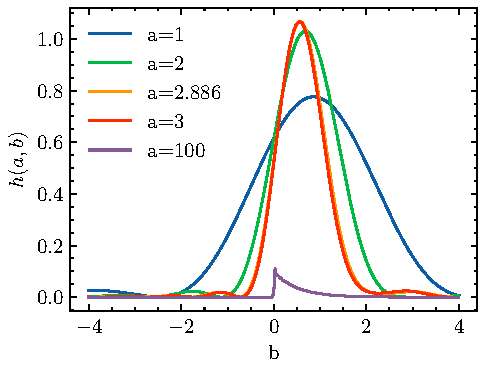
\includegraphics[width=\textwidth]{./img/bk-factor.pdf}
\end{subfigure}
\hspace{0.2cm}
\begin{subfigure}[b]{0.48\textwidth}
	\small
	% This file was created with tikzplotlib v0.10.1.
\begin{tikzpicture}

\definecolor{darkgray176}{RGB}{176,176,176}

\begin{axis}[
colorbar,
colorbar style={ytick={0,0.2,0.4,0.6,0.8,1,1.2},yticklabels={
  \(\displaystyle {0.0}\),
  \(\displaystyle {0.2}\),
  \(\displaystyle {0.4}\),
  \(\displaystyle {0.6}\),
  \(\displaystyle {0.8}\),
  \(\displaystyle {1.0}\),
  \(\displaystyle {1.2}\)
},ylabel={}},
colormap={mymap}{[1pt]
 rgb(0pt)=(0.001462,0.000466,0.013866);
  rgb(1pt)=(0.002267,0.00127,0.01857);
  rgb(2pt)=(0.003299,0.002249,0.024239);
  rgb(3pt)=(0.004547,0.003392,0.030909);
  rgb(4pt)=(0.006006,0.004692,0.038558);
  rgb(5pt)=(0.007676,0.006136,0.046836);
  rgb(6pt)=(0.009561,0.007713,0.055143);
  rgb(7pt)=(0.011663,0.009417,0.06346);
  rgb(8pt)=(0.013995,0.011225,0.071862);
  rgb(9pt)=(0.016561,0.013136,0.080282);
  rgb(10pt)=(0.019373,0.015133,0.088767);
  rgb(11pt)=(0.022447,0.017199,0.097327);
  rgb(12pt)=(0.025793,0.019331,0.10593);
  rgb(13pt)=(0.029432,0.021503,0.114621);
  rgb(14pt)=(0.033385,0.023702,0.123397);
  rgb(15pt)=(0.037668,0.025921,0.132232);
  rgb(16pt)=(0.042253,0.028139,0.141141);
  rgb(17pt)=(0.046915,0.030324,0.150164);
  rgb(18pt)=(0.051644,0.032474,0.159254);
  rgb(19pt)=(0.056449,0.034569,0.168414);
  rgb(20pt)=(0.06134,0.03659,0.177642);
  rgb(21pt)=(0.066331,0.038504,0.186962);
  rgb(22pt)=(0.071429,0.040294,0.196354);
  rgb(23pt)=(0.076637,0.041905,0.205799);
  rgb(24pt)=(0.081962,0.043328,0.215289);
  rgb(25pt)=(0.087411,0.044556,0.224813);
  rgb(26pt)=(0.09299,0.045583,0.234358);
  rgb(27pt)=(0.098702,0.046402,0.243904);
  rgb(28pt)=(0.104551,0.047008,0.25343);
  rgb(29pt)=(0.110536,0.047399,0.262912);
  rgb(30pt)=(0.116656,0.047574,0.272321);
  rgb(31pt)=(0.122908,0.047536,0.281624);
  rgb(32pt)=(0.129285,0.047293,0.290788);
  rgb(33pt)=(0.135778,0.046856,0.299776);
  rgb(34pt)=(0.142378,0.046242,0.308553);
  rgb(35pt)=(0.149073,0.045468,0.317085);
  rgb(36pt)=(0.15585,0.044559,0.325338);
  rgb(37pt)=(0.162689,0.043554,0.333277);
  rgb(38pt)=(0.169575,0.042489,0.340874);
  rgb(39pt)=(0.176493,0.041402,0.348111);
  rgb(40pt)=(0.183429,0.040329,0.354971);
  rgb(41pt)=(0.190367,0.039309,0.361447);
  rgb(42pt)=(0.197297,0.0384,0.367535);
  rgb(43pt)=(0.204209,0.037632,0.373238);
  rgb(44pt)=(0.211095,0.03703,0.378563);
  rgb(45pt)=(0.217949,0.036615,0.383522);
  rgb(46pt)=(0.224763,0.036405,0.388129);
  rgb(47pt)=(0.231538,0.036405,0.3924);
  rgb(48pt)=(0.238273,0.036621,0.396353);
  rgb(49pt)=(0.244967,0.037055,0.400007);
  rgb(50pt)=(0.25162,0.037705,0.403378);
  rgb(51pt)=(0.258234,0.038571,0.406485);
  rgb(52pt)=(0.26481,0.039647,0.409345);
  rgb(53pt)=(0.271347,0.040922,0.411976);
  rgb(54pt)=(0.27785,0.042353,0.414392);
  rgb(55pt)=(0.284321,0.043933,0.416608);
  rgb(56pt)=(0.290763,0.045644,0.418637);
  rgb(57pt)=(0.297178,0.04747,0.420491);
  rgb(58pt)=(0.303568,0.049396,0.422182);
  rgb(59pt)=(0.309935,0.051407,0.423721);
  rgb(60pt)=(0.316282,0.05349,0.425116);
  rgb(61pt)=(0.32261,0.055634,0.426377);
  rgb(62pt)=(0.328921,0.057827,0.427511);
  rgb(63pt)=(0.335217,0.06006,0.428524);
  rgb(64pt)=(0.3415,0.062325,0.429425);
  rgb(65pt)=(0.347771,0.064616,0.430217);
  rgb(66pt)=(0.354032,0.066925,0.430906);
  rgb(67pt)=(0.360284,0.069247,0.431497);
  rgb(68pt)=(0.366529,0.071579,0.431994);
  rgb(69pt)=(0.372768,0.073915,0.4324);
  rgb(70pt)=(0.379001,0.076253,0.432719);
  rgb(71pt)=(0.385228,0.078591,0.432955);
  rgb(72pt)=(0.391453,0.080927,0.433109);
  rgb(73pt)=(0.397674,0.083257,0.433183);
  rgb(74pt)=(0.403894,0.08558,0.433179);
  rgb(75pt)=(0.410113,0.087896,0.433098);
  rgb(76pt)=(0.416331,0.090203,0.432943);
  rgb(77pt)=(0.422549,0.092501,0.432714);
  rgb(78pt)=(0.428768,0.09479,0.432412);
  rgb(79pt)=(0.434987,0.097069,0.432039);
  rgb(80pt)=(0.441207,0.099338,0.431594);
  rgb(81pt)=(0.447428,0.101597,0.43108);
  rgb(82pt)=(0.453651,0.103848,0.430498);
  rgb(83pt)=(0.459875,0.106089,0.429846);
  rgb(84pt)=(0.4661,0.108322,0.429125);
  rgb(85pt)=(0.472328,0.110547,0.428334);
  rgb(86pt)=(0.478558,0.112764,0.427475);
  rgb(87pt)=(0.484789,0.114974,0.426548);
  rgb(88pt)=(0.491022,0.117179,0.425552);
  rgb(89pt)=(0.497257,0.119379,0.424488);
  rgb(90pt)=(0.503493,0.121575,0.423356);
  rgb(91pt)=(0.50973,0.123769,0.422156);
  rgb(92pt)=(0.515967,0.12596,0.420887);
  rgb(93pt)=(0.522206,0.12815,0.419549);
  rgb(94pt)=(0.528444,0.130341,0.418142);
  rgb(95pt)=(0.534683,0.132534,0.416667);
  rgb(96pt)=(0.54092,0.134729,0.415123);
  rgb(97pt)=(0.547157,0.136929,0.413511);
  rgb(98pt)=(0.553392,0.139134,0.411829);
  rgb(99pt)=(0.559624,0.141346,0.410078);
  rgb(100pt)=(0.565854,0.143567,0.408258);
  rgb(101pt)=(0.572081,0.145797,0.406369);
  rgb(102pt)=(0.578304,0.148039,0.404411);
  rgb(103pt)=(0.584521,0.150294,0.402385);
  rgb(104pt)=(0.590734,0.152563,0.40029);
  rgb(105pt)=(0.59694,0.154848,0.398125);
  rgb(106pt)=(0.603139,0.157151,0.395891);
  rgb(107pt)=(0.60933,0.159474,0.393589);
  rgb(108pt)=(0.615513,0.161817,0.391219);
  rgb(109pt)=(0.621685,0.164184,0.388781);
  rgb(110pt)=(0.627847,0.166575,0.386276);
  rgb(111pt)=(0.633998,0.168992,0.383704);
  rgb(112pt)=(0.640135,0.171438,0.381065);
  rgb(113pt)=(0.64626,0.173914,0.378359);
  rgb(114pt)=(0.652369,0.176421,0.375586);
  rgb(115pt)=(0.658463,0.178962,0.372748);
  rgb(116pt)=(0.66454,0.181539,0.369846);
  rgb(117pt)=(0.670599,0.184153,0.366879);
  rgb(118pt)=(0.676638,0.186807,0.363849);
  rgb(119pt)=(0.682656,0.189501,0.360757);
  rgb(120pt)=(0.688653,0.192239,0.357603);
  rgb(121pt)=(0.694627,0.195021,0.354388);
  rgb(122pt)=(0.700576,0.197851,0.351113);
  rgb(123pt)=(0.7065,0.200728,0.347777);
  rgb(124pt)=(0.712396,0.203656,0.344383);
  rgb(125pt)=(0.718264,0.206636,0.340931);
  rgb(126pt)=(0.724103,0.20967,0.337424);
  rgb(127pt)=(0.729909,0.212759,0.333861);
  rgb(128pt)=(0.735683,0.215906,0.330245);
  rgb(129pt)=(0.741423,0.219112,0.326576);
  rgb(130pt)=(0.747127,0.222378,0.322856);
  rgb(131pt)=(0.752794,0.225706,0.319085);
  rgb(132pt)=(0.758422,0.229097,0.315266);
  rgb(133pt)=(0.76401,0.232554,0.311399);
  rgb(134pt)=(0.769556,0.236077,0.307485);
  rgb(135pt)=(0.775059,0.239667,0.303526);
  rgb(136pt)=(0.780517,0.243327,0.299523);
  rgb(137pt)=(0.785929,0.247056,0.295477);
  rgb(138pt)=(0.791293,0.250856,0.29139);
  rgb(139pt)=(0.796607,0.254728,0.287264);
  rgb(140pt)=(0.801871,0.258674,0.283099);
  rgb(141pt)=(0.807082,0.262692,0.278898);
  rgb(142pt)=(0.812239,0.266786,0.274661);
  rgb(143pt)=(0.817341,0.270954,0.27039);
  rgb(144pt)=(0.822386,0.275197,0.266085);
  rgb(145pt)=(0.827372,0.279517,0.26175);
  rgb(146pt)=(0.832299,0.283913,0.257383);
  rgb(147pt)=(0.837165,0.288385,0.252988);
  rgb(148pt)=(0.841969,0.292933,0.248564);
  rgb(149pt)=(0.846709,0.297559,0.244113);
  rgb(150pt)=(0.851384,0.30226,0.239636);
  rgb(151pt)=(0.855992,0.307038,0.235133);
  rgb(152pt)=(0.860533,0.311892,0.230606);
  rgb(153pt)=(0.865006,0.316822,0.226055);
  rgb(154pt)=(0.869409,0.321827,0.221482);
  rgb(155pt)=(0.873741,0.326906,0.216886);
  rgb(156pt)=(0.878001,0.33206,0.212268);
  rgb(157pt)=(0.882188,0.337287,0.207628);
  rgb(158pt)=(0.886302,0.342586,0.202968);
  rgb(159pt)=(0.890341,0.347957,0.198286);
  rgb(160pt)=(0.894305,0.353399,0.193584);
  rgb(161pt)=(0.898192,0.358911,0.18886);
  rgb(162pt)=(0.902003,0.364492,0.184116);
  rgb(163pt)=(0.905735,0.37014,0.17935);
  rgb(164pt)=(0.90939,0.375856,0.174563);
  rgb(165pt)=(0.912966,0.381636,0.169755);
  rgb(166pt)=(0.916462,0.387481,0.164924);
  rgb(167pt)=(0.919879,0.393389,0.16007);
  rgb(168pt)=(0.923215,0.399359,0.155193);
  rgb(169pt)=(0.92647,0.405389,0.150292);
  rgb(170pt)=(0.929644,0.411479,0.145367);
  rgb(171pt)=(0.932737,0.417627,0.140417);
  rgb(172pt)=(0.935747,0.423831,0.13544);
  rgb(173pt)=(0.938675,0.430091,0.130438);
  rgb(174pt)=(0.941521,0.436405,0.125409);
  rgb(175pt)=(0.944285,0.442772,0.120354);
  rgb(176pt)=(0.946965,0.449191,0.115272);
  rgb(177pt)=(0.949562,0.45566,0.110164);
  rgb(178pt)=(0.952075,0.462178,0.105031);
  rgb(179pt)=(0.954506,0.468744,0.099874);
  rgb(180pt)=(0.956852,0.475356,0.094695);
  rgb(181pt)=(0.959114,0.482014,0.089499);
  rgb(182pt)=(0.961293,0.488716,0.084289);
  rgb(183pt)=(0.963387,0.495462,0.079073);
  rgb(184pt)=(0.965397,0.502249,0.073859);
  rgb(185pt)=(0.967322,0.509078,0.068659);
  rgb(186pt)=(0.969163,0.515946,0.063488);
  rgb(187pt)=(0.970919,0.522853,0.058367);
  rgb(188pt)=(0.97259,0.529798,0.053324);
  rgb(189pt)=(0.974176,0.53678,0.048392);
  rgb(190pt)=(0.975677,0.543798,0.043618);
  rgb(191pt)=(0.977092,0.55085,0.03905);
  rgb(192pt)=(0.978422,0.557937,0.034931);
  rgb(193pt)=(0.979666,0.565057,0.031409);
  rgb(194pt)=(0.980824,0.572209,0.028508);
  rgb(195pt)=(0.981895,0.579392,0.02625);
  rgb(196pt)=(0.982881,0.586606,0.024661);
  rgb(197pt)=(0.983779,0.593849,0.02377);
  rgb(198pt)=(0.984591,0.601122,0.023606);
  rgb(199pt)=(0.985315,0.608422,0.024202);
  rgb(200pt)=(0.985952,0.61575,0.025592);
  rgb(201pt)=(0.986502,0.623105,0.027814);
  rgb(202pt)=(0.986964,0.630485,0.030908);
  rgb(203pt)=(0.987337,0.63789,0.034916);
  rgb(204pt)=(0.987622,0.64532,0.039886);
  rgb(205pt)=(0.987819,0.652773,0.045581);
  rgb(206pt)=(0.987926,0.66025,0.05175);
  rgb(207pt)=(0.987945,0.667748,0.058329);
  rgb(208pt)=(0.987874,0.675267,0.065257);
  rgb(209pt)=(0.987714,0.682807,0.072489);
  rgb(210pt)=(0.987464,0.690366,0.07999);
  rgb(211pt)=(0.987124,0.697944,0.087731);
  rgb(212pt)=(0.986694,0.70554,0.095694);
  rgb(213pt)=(0.986175,0.713153,0.103863);
  rgb(214pt)=(0.985566,0.720782,0.112229);
  rgb(215pt)=(0.984865,0.728427,0.120785);
  rgb(216pt)=(0.984075,0.736087,0.129527);
  rgb(217pt)=(0.983196,0.743758,0.138453);
  rgb(218pt)=(0.982228,0.751442,0.147565);
  rgb(219pt)=(0.981173,0.759135,0.156863);
  rgb(220pt)=(0.980032,0.766837,0.166353);
  rgb(221pt)=(0.978806,0.774545,0.176037);
  rgb(222pt)=(0.977497,0.782258,0.185923);
  rgb(223pt)=(0.976108,0.789974,0.196018);
  rgb(224pt)=(0.974638,0.797692,0.206332);
  rgb(225pt)=(0.973088,0.805409,0.216877);
  rgb(226pt)=(0.971468,0.813122,0.227658);
  rgb(227pt)=(0.969783,0.820825,0.238686);
  rgb(228pt)=(0.968041,0.828515,0.249972);
  rgb(229pt)=(0.966243,0.836191,0.261534);
  rgb(230pt)=(0.964394,0.843848,0.273391);
  rgb(231pt)=(0.962517,0.851476,0.285546);
  rgb(232pt)=(0.960626,0.859069,0.29801);
  rgb(233pt)=(0.95872,0.866624,0.31082);
  rgb(234pt)=(0.956834,0.874129,0.323974);
  rgb(235pt)=(0.954997,0.881569,0.337475);
  rgb(236pt)=(0.953215,0.888942,0.351369);
  rgb(237pt)=(0.951546,0.896226,0.365627);
  rgb(238pt)=(0.950018,0.903409,0.380271);
  rgb(239pt)=(0.948683,0.910473,0.395289);
  rgb(240pt)=(0.947594,0.917399,0.410665);
  rgb(241pt)=(0.946809,0.924168,0.426373);
  rgb(242pt)=(0.946392,0.930761,0.442367);
  rgb(243pt)=(0.946403,0.937159,0.458592);
  rgb(244pt)=(0.946903,0.943348,0.47497);
  rgb(245pt)=(0.947937,0.949318,0.491426);
  rgb(246pt)=(0.949545,0.955063,0.50786);
  rgb(247pt)=(0.95174,0.960587,0.524203);
  rgb(248pt)=(0.954529,0.965896,0.540361);
  rgb(249pt)=(0.957896,0.971003,0.556275);
  rgb(250pt)=(0.961812,0.975924,0.571925);
  rgb(251pt)=(0.966249,0.980678,0.587206);
  rgb(252pt)=(0.971162,0.985282,0.602154);
  rgb(253pt)=(0.976511,0.989753,0.61676);
  rgb(254pt)=(0.982257,0.994109,0.631017);
  rgb(255pt)=(0.988362,0.998364,0.644924)
},
point meta max=1.06749233213328,
point meta min=1.43780715113311e-12,
tick pos=both,
x grid style={darkgray176},
xlabel={\(\displaystyle a\)},
xmin=0.01, xmax=8,
xtick style={color=black},
xtick={0,2,4,6,8},
xticklabels={
  \(\displaystyle {0}\),
  \(\displaystyle {2}\),
  \(\displaystyle {4}\),
  \(\displaystyle {6}\),
  \(\displaystyle {8}\)
},
y grid style={darkgray176},
ylabel={\(\displaystyle b\)},
ymin=-4, ymax=4,
ytick style={color=black},
ytick={-4,-2,0,2,4},
yticklabels={
  \(\displaystyle {\ensuremath{-}4}\),
  \(\displaystyle {\ensuremath{-}2}\),
  \(\displaystyle {0}\),
  \(\displaystyle {2}\),
  \(\displaystyle {4}\)
}
]
\addplot graphics [includegraphics cmd=\pgfimage,xmin=0.01, xmax=8, ymin=-4, ymax=4] {bk-factor-cmap-001.png};
\end{axis}

\end{tikzpicture}

	%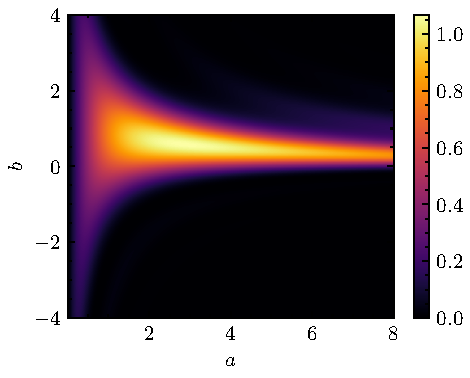
\includegraphics[width=\textwidth]{./img/bk-factor-cmap.pdf}
\end{subfigure}
\hspace{0.8cm}
\caption{Facteur de Boyd-Kleinman : \small dépendance en $b$ pour différentes valeurs de $a$ fixées et profil global}
\label{fig:bk-factor}
\end{figure}

Le profil de $h$ est tracé figure \ref{fig:bk-factor}. Le facteur de Boyd-Kleinman $h$ est maximal pour $a=2.8$ et $b=0.58$, et vaut alors $1.068$. On remarque également que le maximum est assez large en $a$ et se rétrécit en $b$ lorsqu'on se rapproche de la valeur optimale de $a$.

Physiquement, $a\gg1$ (\textit{i.e. $\zr \ll L$}) correspond à un faisceau fortement focalisé. L'intensité est alors importante au point focal, mais décroît rapidement dès que l'on s'en écarte. À l'inverse, $a\ll1$ (\textit{i.e. $\zr \gg L$}) correspond à un faisceau collimaté. L'intensité a alors un maximum moins intense mais est uniforme sur la longueur du cristal. Notons au passage que l'on retrouve bien dans cette limite le résultat pour les ondes planes donné par l'équation (\ref{eq:plane}), en considérant que $h(a,b) \approx a \sinc^2(ab)$ et $\P = \frac{\pi w_0^2}{2} I$.
L'optimum de $a$ correspond à un compromis entre ces deux cas limites, avec une longueur de Rayleigh comparable à la longueur du cristal.
% donnant $\alpha = \frac{\chie^2 \omega^2 L^2}{2 \varepsilon_0 c^3 \pi w_0^2 n_1^2 n_2}$ en passant des intensités aux puissances ($\P = \frac{\pi w_0^2}{2} I$). 

%et sera discuté plus bas en relation avec la réalisation expérimentale du doublage.

%On constate que l'optimum en $a$ est relativement souple, l'optimum $a=2.886$ et $a=3$ donnant essentiellement les mêmes courbes. 

\section{Réalisation de la génération  de seconde harmonique} 

Maintenant que l'on a discuté le principe de la génération de seconde harmonique et déterminé les valeurs optimales des paramètres $a$ et $b$, nous allons présenter la mise en place expérimentale du doublage dans cette section puis étudier les résultats obtenus à la lumière des calculs théoriques dans la section suivante. Tous les règlages sont d'abord faits à basse puissance (autour de $\SI{100}{mW}$) pour des raisons de sécurité ainsi que pour éviter d'endommager le cristal.

\subsection{Choix du cristal doubleur}

Le cristal doubleur choisi pour mon stage est un cristal de niobate de lithium périodiquement pôlé dopé au magnésium (Mgo\hc PPLN). Il présente l'avantage d'avoir un $\chi^{(2)}$ important selon l'axe extraordinaire et donc une bonne efficacité de conversion. En revanche, il présente des effets non-linéaires parasites conduisant notamment à des inhomogénéités d'indice optique et un couplage entre les faisceaux mais présente en revanche une dégradation optique plus importante. Il est donc avantageux lorsque l'on ne cherche pas à produire plus de 2 ou 3 watts de lumière verte, ce qui est notre cas. % En effet, %TODO

Le cristal commandé chez Covesion a une longueur $L=\SI{20}{mm}$ et présente 5 bandes avec des inversions de périodes différentes : $\Lambda = \qtylist[list-units = single]{6.83; 6.86 ; 6.90 ; 6.93 ; 6,96}{\micro\meter}$ (figure \ref{fig:sc}).

\subsection{Montage et alignement} 

\begin{figure}[htpb]
\centering
\hspace*{-0.8cm}
\begin{subfigure}[b]{0.48\textwidth}
	\centering
	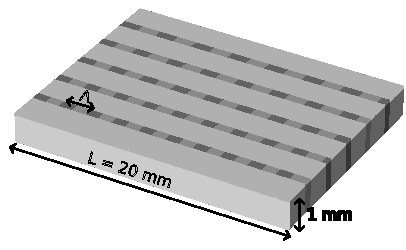
\includegraphics[height=5cm]{./img/cristal.pdf}
	\vspace{0.8cm}
	\caption{Schéma du cristal}
	\label{fig:sc}
\end{subfigure}
\centering
\hspace*{0.4cm}
\begin{subfigure}[b]{0.48\textwidth}
    % This file was created with tikzplotlib v0.10.1.
\begin{tikzpicture}

\definecolor{darkgray176}{RGB}{176,176,176}
\definecolor{limegreen018569}{RGB}{0,185,69}
\definecolor{teal1293165}{RGB}{12,93,165}

\begin{axis}[
legend cell align={left},
legend style={fill opacity=0.8, draw opacity=1, text opacity=1, draw=none},
tick pos=both,
x grid style={darkgray176},
xlabel={distance z à la lentille (\(\displaystyle \unit{cm}\))},
xmin=0, xmax=45,
xtick style={color=black},
xtick={0,10,20,30,40,50},
xticklabels={
  \(\displaystyle {0}\),
  \(\displaystyle {10}\),
  \(\displaystyle {20}\),
  \(\displaystyle {30}\),
  \(\displaystyle {40}\),
  \(\displaystyle {50}\)
},
y grid style={darkgray176},
ylabel={waist (\(\displaystyle \unit{\micro\meter}\))},
ymin=0, ymax=2750,
ytick style={color=black},
ytick={0,500,1000,1500,2000,2500},
yticklabels={
  \(\displaystyle {0}\),
  \(\displaystyle {500}\),
  \(\displaystyle {1000}\),
  \(\displaystyle {1500}\),
  \(\displaystyle {2000}\),
  \(\displaystyle {2500}\)
}
]
\path [draw=teal1293165, very thick]
(axis cs:41.9,1995)
--(axis cs:42.5,1995);

\path [draw=teal1293165, very thick]
(axis cs:27.4,1243)
--(axis cs:28,1243);

\path [draw=teal1293165, very thick]
(axis cs:5.9,100)
--(axis cs:6.5,100);

\path [draw=teal1293165, very thick]
(axis cs:4.4,68)
--(axis cs:5,68);

\path [draw=teal1293165, very thick]
(axis cs:10.1,301)
--(axis cs:10.7,301);

\path [draw=teal1293165, very thick]
(axis cs:3.9,87)
--(axis cs:4.5,87);

\path [draw=teal1293165, very thick]
(axis cs:14.9,535)
--(axis cs:15.5,535);

\path [draw=teal1293165, very thick]
(axis cs:27.9,1290)
--(axis cs:28.5,1290);

\path [draw=teal1293165, very thick]
(axis cs:20.9,910)
--(axis cs:21.5,910);

\path [draw=teal1293165, very thick]
(axis cs:42.2,1895)
--(axis cs:42.2,2095);

\path [draw=teal1293165, very thick]
(axis cs:27.7,1203)
--(axis cs:27.7,1283);

\path [draw=teal1293165, very thick]
(axis cs:6.2,60)
--(axis cs:6.2,140);

\path [draw=teal1293165, very thick]
(axis cs:4.7,28)
--(axis cs:4.7,108);

\path [draw=teal1293165, very thick]
(axis cs:10.4,261)
--(axis cs:10.4,341);

\path [draw=teal1293165, very thick]
(axis cs:4.2,47)
--(axis cs:4.2,127);

\path [draw=teal1293165, very thick]
(axis cs:15.2,495)
--(axis cs:15.2,575);

\path [draw=teal1293165, very thick]
(axis cs:28.2,1250)
--(axis cs:28.2,1330);

\path [draw=teal1293165, very thick]
(axis cs:21.2,870)
--(axis cs:21.2,950);

\addplot [very thick, limegreen018569, dashed]
table {%
0 270.726301163772
0.918367346938776 222.721199828545
1.83673469387755 175.632620773748
2.75510204081633 130.456828193017
3.6734693877551 90.1178810228514
4.59183673469388 64.4481408068083
5.51020408163265 71.5260452031186
6.42857142857143 104.921253075256
7.3469387755102 147.7533264157
8.26530612244898 193.865168357974
9.18367346938776 241.384430843346
10.1020408163265 289.619172915409
11.0204081632653 338.263461080832
11.9387755102041 387.162956389298
12.8571428571429 436.231844795124
13.7755102040816 485.418759363658
14.6938775510204 534.6911289581
15.6122448979592 584.027325342197
16.530612244898 633.412434375718
17.4489795918367 682.835843532488
18.3673469387755 732.289798043926
19.2857142857143 781.768501118613
20.2040816326531 831.267533516624
21.1224489795918 880.783467789853
22.0408163265306 930.313605135691
22.9591836734694 979.855791728942
23.8775510204082 1029.40828789381
24.7959183673469 1078.96967320668
25.7142857142857 1128.53877652943
26.6326530612245 1178.11462365802
27.5510204081633 1227.69639762392
28.469387755102 1277.28340822082
29.3877551020408 1326.87506835012
30.3061224489796 1376.47087547018
31.2244897959184 1426.07039690952
32.1428571428571 1475.6732581372
33.0612244897959 1525.27913331835
33.9795918367347 1574.88773765212
34.8979591836735 1624.49882111167
35.8163265306122 1674.1121632958
36.734693877551 1723.72756916869
37.6530612244898 1773.34486551404
38.5714285714286 1822.96389796764
39.4897959183673 1872.58452852128
40.4081632653061 1922.20663341293
41.3265306122449 1971.83010133522
42.2448979591837 2021.45483190749
43.1632653061224 2071.08073436749
44.0816326530612 2120.70772644647
45 2170.33573339861
};
\addlegendentry{$w_0 = \SI{62.6}{\micro\meter}$, $z_0 = \SI{4.9}{cm}$}
\addplot [very thick, teal1293165, mark=+, mark size=1.5, mark options={solid}, only marks]
table {%
42.2 1995
27.7 1243
6.2 100
4.7 68
10.4 301
4.2 87
15.2 535
28.2 1290
21.2 910
};
\addlegendentry{waist mesuré}
\end{axis}

\end{tikzpicture}

	\vspace{-0.5cm}
    \caption{Profil du faisceau incident sur le cristal}
    \label{fig:wincident}
\end{subfigure}
\caption{}
\end{figure}

Tout d'abord, on place une lentille devant le cristal afin d'obtenir un faisceau incident focalisé au centre du cristal et avec le bon souhaité (conformément à la valeur de $a$ voulue).

Les premières mesures ont été réalisées avec le faisceau issu de la fibre à cristaux photoniques et une lentille de focale $\SI{5}{cm}$, sachant que le faisceau incident sur la lentille est collimaté. Le profil du faisceau obtenu a été vérifié à la caméra en mesurant le waist à différentes positions (figure \ref{fig:wincident}). Avec le waist obtenu de $\SI{62.6}{\micro\meter}$, $a=\frac{L}{2\zr}=0.4$ ($\zr = \frac{n_1 \pi w_0^2}{\lambda_1} = \SI{2.4}{cm}$), 
 ce qui est suboptimal mais corresond à un pic en $b$ plus large et donc plus facile à trouver.

 Il s'agit ensuite d'optimiser la température du cristal (contrôlée à l'aide d'un four Covesion) et l'alignement du faisceau incident à l'aide des deux miroirs (cf. schéma figure \ref{fig:montage}). Pour estimer la température à laquelle se trouve l'optimum, on utilise une estimation des indices optiques $n_1$ et $n_2$ en fonction de la température à partir d'une équation dite de Sellmeier, pour laquelle on a pris les coefficients correspondants à un cristal de niobate de lithium congruent dopé à $\SI{5}{\percent}$ \ncite{gayer,covesion}, et qui est tracée figure \ref{fig:sellmeier}. La température optimale calculée de la sorte est donnée figure \ref{fig:lp}. Pour $\Lambda = \SI{6.9}{\micro\meter}$, on s'attend à $\SI{66}{\celsius}$.

\begin{figure}[htpb] 
\centering
\hspace*{-0.8cm}
\begin{subfigure}[b]{0.48\textwidth}
	\centering
	% This file was created with tikzplotlib v0.10.1.
\begin{tikzpicture}

\definecolor{darkgray176}{RGB}{176,176,176}
\definecolor{teal1293165}{RGB}{12,93,165}

\begin{axis}[
tick pos=both,
x grid style={darkgray176},
xlabel={T (°C)},
xmin=45, xmax=155,
xtick style={color=black},
xtick={40,60,80,100,120,140,160},
xticklabels={
  \(\displaystyle {40}\),
  \(\displaystyle {60}\),
  \(\displaystyle {80}\),
  \(\displaystyle {100}\),
  \(\displaystyle {120}\),
  \(\displaystyle {140}\),
  \(\displaystyle {160}\)
},
y grid style={darkgray176},
ylabel={\(\displaystyle n_2-n_1\) \(\displaystyle \left(\times 10^{-2}\right)\)},
ymin=7.6629850784832, ymax=7.89936722344637,
ytick style={color=black},
ytick={7.65,7.7,7.75,7.8,7.85,7.9},
yticklabels={
  \(\displaystyle {7.65}\),
  \(\displaystyle {7.70}\),
  \(\displaystyle {7.75}\),
  \(\displaystyle {7.80}\),
  \(\displaystyle {7.85}\),
  \(\displaystyle {7.90}\)
}
]
\addplot [very thick, teal1293165]
table {%
50 7.67372972143607
50.2004008016032 7.67410055301299
50.4008016032064 7.6744716219225
50.6012024048096 7.67484292818015
50.8016032064128 7.67521447180144
51.002004008016 7.67558625280187
51.2024048096192 7.67595827119703
51.4028056112224 7.67633052700245
51.6032064128256 7.67670302023364
51.8036072144289 7.67707575090624
52.0040080160321 7.67744871903582
52.2044088176353 7.67782192463806
52.4048096192385 7.67819536772842
52.6052104208417 7.67856904832276
52.8056112224449 7.67894296643661
53.0060120240481 7.67931712208565
53.2064128256513 7.67969151528551
53.4068136272545 7.6800661460521
53.6072144288577 7.68044101440086
53.8076152304609 7.68081612034774
54.0080160320641 7.68119146390829
54.2084168336673 7.68156704509853
54.4088176352705 7.68194286393391
54.6092184368737 7.68231892043048
54.809619238477 7.68269521460399
55.0100200400802 7.68307174647016
55.2104208416834 7.68344851604494
55.4108216432866 7.68382552334415
55.6112224448898 7.68420276838357
55.811623246493 7.68458025117922
56.0120240480962 7.68495797174684
56.2124248496994 7.68533593010248
56.4128256513026 7.68571412626198
56.6132264529058 7.68609256024129
56.813627254509 7.68647123205644
57.0140280561122 7.68685014172328
57.2144288577154 7.68722928925785
57.4148296593186 7.68760867467617
57.6152304609218 7.68798829799429
57.8156312625251 7.68836815922813
58.0160320641283 7.68874825839378
58.2164328657315 7.68912859550737
58.4168336673347 7.68950917058491
58.6172344689379 7.68988998364253
58.8176352705411 7.69027103469626
59.0180360721443 7.69065232376223
59.2184368737475 7.69103385085668
59.4188376753507 7.69141561599564
59.6192384769539 7.69179761919534
59.8196392785571 7.69217986047197
60.0200400801603 7.6925623398417
60.2204408817635 7.6929450573207
60.4208416833667 7.69332801292535
60.6212424849699 7.69371120667177
60.8216432865731 7.69409463857613
61.0220440881764 7.69447830865491
61.2224448897796 7.69486221692426
61.4228456913828 7.69524636340053
61.623246492986 7.69563074810002
61.8236472945892 7.69601537103908
62.0240480961924 7.69640023223404
62.2244488977956 7.69678533170128
62.4248496993988 7.69717066945721
62.625250501002 7.69755624551811
62.8256513026052 7.69794205990051
63.0260521042084 7.69832811262079
63.2264529058116 7.69871440369543
63.4268537074148 7.69910093314077
63.627254509018 7.69948770097342
63.8276553106212 7.69987470720976
64.0280561122244 7.70026195186642
64.2284569138277 7.70064943495981
64.4288577154309 7.7010371565065
64.6292585170341 7.70142511652296
64.8296593186373 7.70181331502586
65.0300601202405 7.7022017520318
65.2304609218437 7.70259042755725
65.4308617234469 7.70297934161892
65.6312625250501 7.70336849423341
65.8316633266533 7.70375788541733
66.0320641282565 7.70414751518742
66.2324649298597 7.70453738356025
66.4328657314629 7.70492749055252
66.6332665330661 7.705317836181
66.8336673346693 7.70570842046241
67.0340681362725 7.70609924341339
67.2344689378758 7.70649030505077
67.434869739479 7.7068816053913
67.6352705410822 7.70727314445177
67.8356713426854 7.70766492224886
68.0360721442886 7.70805693879959
68.2364729458918 7.7084491941207
68.436873747495 7.70884168822894
68.6372745490982 7.70923442114126
68.8376753507014 7.70962739287455
69.0380761523046 7.71002060344563
69.2384769539078 7.71041405287143
69.438877755511 7.7108077411689
69.6392785571142 7.71120166835497
69.8396793587174 7.71159583444665
70.0400801603206 7.71199023946076
70.2404809619239 7.71238488341437
70.4408817635271 7.71277976632447
70.6412825651303 7.71317488820813
70.8416833667335 7.7135702490823
71.0420841683367 7.71396584896404
71.2424849699399 7.71436168787045
71.4428857715431 7.71475776581863
71.6432865731463 7.71515408282561
71.8436873747495 7.71555063890847
72.0440881763527 7.71594743408444
72.2444889779559 7.71634446837064
72.4448897795591 7.71674174178414
72.6452905811623 7.71713925434225
72.8456913827655 7.71753700606199
73.0460921843687 7.71793499696072
73.2464929859719 7.71833322705557
73.4468937875751 7.71873169636383
73.6472945891784 7.71913040490269
73.8476953907816 7.71952935268949
74.0480961923848 7.71992853974148
74.248496993988 7.72032796607598
74.4488977955912 7.72072763171026
74.6492985971944 7.72112753666163
74.8496993987976 7.72152768094752
75.0501002004008 7.72192806458527
75.250501002004 7.72232868759222
75.4509018036072 7.72272954998585
75.6513026052104 7.72313065178345
75.8517034068136 7.7235319930026
76.0521042084168 7.72393357366061
76.25250501002 7.72433539377495
76.4529058116233 7.7247374533632
76.6533066132264 7.7251397524428
76.8537074148297 7.72554229103117
77.0541082164329 7.72594506914595
77.2545090180361 7.72634808680457
77.4549098196393 7.72675134402476
77.6553106212425 7.72715484082389
77.8557114228457 7.72755857721967
78.0561122244489 7.72796255322974
78.2565130260521 7.72836676887159
78.4569138276553 7.72877122416298
78.6573146292585 7.7291759191215
78.8577154308617 7.72958085376474
79.0581162324649 7.72998602811055
79.2585170340681 7.73039144217651
79.4589178356713 7.73079709598039
79.6593186372746 7.73120298953991
79.8597194388778 7.73160912287287
80.060120240481 7.73201549599691
80.2605210420842 7.73242210892993
80.4609218436874 7.73282896168968
80.6613226452906 7.73323605429397
80.8617234468938 7.73364338676061
81.062124248497 7.7340509591076
81.2625250501002 7.73445877135255
81.4629258517034 7.73486682351359
81.6633266533066 7.73527511560843
81.8637274549098 7.73568364765498
82.064128256513 7.7360924196713
82.2645290581162 7.7365014316753
82.4649298597194 7.73691068368492
82.6653306613227 7.73732017571809
82.8657314629259 7.73772990779285
83.0661322645291 7.73813987992722
83.2665330661323 7.7385500921392
83.4669338677355 7.73896054444685
83.6673346693387 7.73937123686821
83.8677354709419 7.73978216942139
84.0681362725451 7.74019334212439
84.2685370741483 7.74060475499545
84.4689378757515 7.74101640805265
84.6693386773547 7.74142830131406
84.8697394789579 7.74184043479789
85.0701402805611 7.74225280852239
85.2705410821643 7.74266542250563
85.4709418837675 7.74307827676584
85.6713426853707 7.74349137132133
85.8717434869739 7.74390470619015
86.0721442885772 7.74431828139082
86.2725450901804 7.74473209694144
86.4729458917836 7.74514615286028
86.6733466933868 7.74556044916581
86.87374749499 7.74597498587615
87.0741482965932 7.74638976300976
87.2745490981964 7.746804780585
87.4749498997996 7.74722003862016
87.6753507014028 7.74763553713371
87.875751503006 7.748051276144
88.0761523046092 7.74846725566953
88.2765531062124 7.74888347572871
88.4769539078156 7.7492999363399
88.6773547094188 7.74971663752173
88.877755511022 7.75013357929253
89.0781563126253 7.75055076167099
89.2785571142284 7.75096818467542
89.4789579158317 7.75138584832451
89.6793587174349 7.75180375263673
89.8797595190381 7.75222189763074
90.0801603206413 7.75264028332505
90.2805611222445 7.75305890973832
90.4809619238477 7.75347777688915
90.6813627254509 7.75389688479615
90.8817635270541 7.75431623347806
91.0821643286573 7.75473582295345
91.2825651302605 7.7551556532411
91.4829659318637 7.75557572435961
91.6833667334669 7.75599603632786
91.8837675350701 7.75641658916442
92.0841683366733 7.75683738288819
92.2845691382766 7.75725841751784
92.4849699398798 7.75767969307224
92.685370741483 7.75810120957012
92.8857715430862 7.75852296703032
93.0861723446894 7.75894496547176
93.2865731462926 7.75936720491321
93.4869739478958 7.75978968537361
93.687374749499 7.76021240687181
93.8877755511022 7.7606353694267
94.0881763527054 7.76105857305729
94.2885771543086 7.76148201778248
94.4889779559118 7.76190570362116
94.689378757515 7.76232963059238
94.8897795591182 7.76275379871523
95.0901803607214 7.76317820800849
95.2905811623247 7.76360285849131
95.4909819639279 7.76402775018279
95.6913827655311 7.76445288310188
95.8917835671343 7.76487825726782
96.0921843687375 7.76530387269951
96.2925851703407 7.7657297294162
96.4929859719439 7.76615582743698
96.6933867735471 7.76658216678099
96.8937875751503 7.76700874746736
97.0941883767535 7.76743556951534
97.2945891783567 7.76786263294413
97.4949899799599 7.76828993777285
97.6953907815631 7.76871748402086
97.8957915831663 7.76914527170729
98.0961923847695 7.76957330085151
98.2965931863727 7.77000157147278
98.496993987976 7.7704300835904
98.6973947895792 7.77085883722357
98.8977955911824 7.77128783239185
99.0981963927856 7.77171706911437
99.2985971943888 7.77214654741067
99.498997995992 7.77257626730008
99.6993987975952 7.77300622880199
99.8997995991984 7.77343643193578
100.100200400802 7.77386687672097
100.300601202405 7.77429756317698
100.501002004008 7.7747284913233
100.701402805611 7.77515966117939
100.901803607214 7.77559107276482
101.102204408818 7.77602272609901
101.302605210421 7.77645462120167
101.503006012024 7.77688675809221
101.703406813627 7.77731913679021
101.90380761523 7.77775175731539
102.104208416834 7.77818461968729
102.304609218437 7.7786177239255
102.50501002004 7.77905107004973
102.705410821643 7.77948465807961
102.905811623246 7.77991848803485
103.10621242485 7.78035255993514
103.306613226453 7.78078687380019
103.507014028056 7.78122142964977
103.707414829659 7.78165622750357
103.907815631263 7.78209126738134
104.108216432866 7.78252654930305
104.308617234469 7.78296207328824
104.509018036072 7.78339783935698
104.709418837675 7.78383384752894
104.909819639279 7.78427009782403
105.110220440882 7.78470659026214
105.310621242485 7.78514332486315
105.511022044088 7.78558030164702
105.711422845691 7.78601752063359
105.911823647295 7.78645498184289
106.112224448898 7.78689268529482
106.312625250501 7.7873306310094
106.513026052104 7.78776881900662
106.713426853707 7.78820724930642
106.913827655311 7.78864592192896
107.114228456914 7.78908483689422
107.314629258517 7.78952399422228
107.51503006012 7.7899633939333
107.715430861723 7.79040303604726
107.915831663327 7.79084292058432
108.11623246493 7.79128304756465
108.316633266533 7.79172341700844
108.517034068136 7.79216402893579
108.717434869739 7.79260488336693
108.917835671343 7.79304598032202
109.118236472946 7.79348731982141
109.318637274549 7.79392890188522
109.519038076152 7.79437072653382
109.719438877756 7.79481279378746
109.919839679359 7.79525510366632
110.120240480962 7.7956976561909
110.320641282565 7.79614045138142
110.521042084168 7.79658348925829
110.721442885772 7.79702676984186
110.921843687375 7.79747029315252
111.122244488978 7.79791405921069
111.322645290581 7.79835806803675
111.523046092184 7.79880231965118
111.723446893788 7.79924681407445
111.923847695391 7.79969155132703
112.124248496994 7.80013653142944
112.324649298597 7.8005817544021
112.5250501002 7.80102722026563
112.725450901804 7.80147292904059
112.925851703407 7.80191888074753
113.12625250501 7.80236507540706
113.326653306613 7.8028115130397
113.527054108216 7.80325819366618
113.72745490982 7.80370511730704
113.927855711423 7.80415228398303
114.128256513026 7.80459969371479
114.328657314629 7.80504734652294
114.529058116232 7.80549524242833
114.729458917836 7.80594338145164
114.929859719439 7.80639176361357
115.130260521042 7.80684038893495
115.330661322645 7.80728925743657
115.531062124248 7.80773836913915
115.731462925852 7.80818772406358
115.931863727455 7.80863732223067
116.132264529058 7.8090871636614
116.332665330661 7.80953724837641
116.533066132265 7.80998757639684
116.733466933868 7.81043814774347
116.933867735471 7.81088896243722
117.134268537074 7.81134002049915
117.334669338677 7.81179132195011
117.535070140281 7.81224286681104
117.735470941884 7.81269465510315
117.935871743487 7.81314668684736
118.13627254509 7.81359896206464
118.336673346693 7.81405148077616
118.537074148297 7.81450424300294
118.7374749499 7.81495724876602
118.937875751503 7.81541049808663
119.138276553106 7.81586399098586
119.338677354709 7.81631772748486
119.539078156313 7.8167717076048
119.739478957916 7.81722593136682
119.939879759519 7.8176803987922
120.140280561122 7.81813510990208
120.340681362725 7.81859006471786
120.541082164329 7.81904526326067
120.741482965932 7.8195007055518
120.941883767535 7.81995639161255
121.142284569138 7.82041232146424
121.342685370741 7.82086849512829
121.543086172345 7.82132491262599
121.743486973948 7.82178157397868
121.943887775551 7.82223847920775
122.144288577154 7.82269562833471
122.344689378758 7.8231530213809
122.545090180361 7.82361065836779
122.745490981964 7.82406853931681
122.945891783567 7.82452666424951
123.14629258517 7.82498503318734
123.346693386774 7.82544364615188
123.547094188377 7.82590250316457
123.74749498998 7.8263616042471
123.947895791583 7.826820949421
124.148296593186 7.8272805387078
124.34869739479 7.8277403721291
124.549098196393 7.82820044970669
124.749498997996 7.82866077146207
124.949899799599 7.829121337417
125.150300601202 7.82958214759315
125.350701402806 7.83004320201219
125.551102204409 7.83050450069585
125.751503006012 7.83096604366595
125.951903807615 7.83142783094419
126.152304609218 7.83188986255237
126.352705410822 7.83235213851228
126.553106212425 7.83281465884569
126.753507014028 7.83327742357462
126.953907815631 7.83374043272071
127.154308617234 7.83420368630603
127.354709418838 7.83466718435233
127.555110220441 7.83513092688159
127.755511022044 7.83559491391572
127.955911823647 7.83605914547669
128.156312625251 7.83652362158644
128.356713426854 7.836988342267
128.557114228457 7.8374533075404
128.75751503006 7.83791851742861
128.957915831663 7.83838397195376
129.158316633267 7.83884967113782
129.35871743487 7.83931561500291
129.559118236473 7.83978180357114
129.759519038076 7.84024823686464
129.959919839679 7.84071491490557
130.160320641283 7.84118183771603
130.360721442886 7.84164900531832
130.561122244489 7.84211641773451
130.761523046092 7.84258407498686
130.961923847695 7.8430519770976
131.162324649299 7.84352012408904
131.362725450902 7.84398851598342
131.563126252505 7.84445715280304
131.763527054108 7.84492603457019
131.963927855711 7.8453951613072
132.164328657315 7.84586453303655
132.364729458918 7.84633414978044
132.565130260521 7.84680401156126
132.765531062124 7.8472741184016
132.965931863727 7.84774447032373
133.166332665331 7.84821506735018
133.366733466934 7.84868590950336
133.567134268537 7.84915699680573
133.76753507014 7.84962832927989
133.967935871743 7.85009990694832
134.168336673347 7.85057172983361
134.36873747495 7.85104379795825
134.569138276553 7.85151611134483
134.769539078156 7.85198867001604
134.96993987976 7.85246147399441
135.170340681363 7.85293452330258
135.370741482966 7.85340781796324
135.571142284569 7.85388135799914
135.771543086172 7.85435514343287
135.971943887776 7.85482917428717
136.172344689379 7.85530345058478
136.372745490982 7.85577797234853
136.573146292585 7.85625273960115
136.773547094188 7.85672775236539
136.973947895792 7.85720301066415
137.174348697395 7.85767851452017
137.374749498998 7.85815426395637
137.575150300601 7.85863025899562
137.775551102204 7.8591064996608
137.975951903808 7.8595829859748
138.176352705411 7.86005971796064
138.376753507014 7.86053669564115
138.577154308617 7.86101391903942
138.77755511022 7.86149138817831
138.977955911824 7.86196910308092
139.178356713427 7.86244706377031
139.37875751503 7.86292527026942
139.579158316633 7.86340372260144
139.779559118236 7.86388242078941
139.97995991984 7.8643613648564
140.180360721443 7.86484055482561
140.380761523046 7.86531999072011
140.581162324649 7.86579967256311
140.781563126253 7.86627960037785
140.981963927856 7.8667597741874
141.182364729459 7.86724019401515
141.382765531062 7.86772085988421
141.583166332665 7.86820177181791
141.783567134269 7.86868292983955
141.983967935872 7.86916433397242
142.184368737475 7.86964598423983
142.384769539078 7.87012788066512
142.585170340681 7.87061002327167
142.785571142285 7.87109241208288
142.985971943888 7.8715750471221
143.186372745491 7.87205792841288
143.386773547094 7.87254105597852
143.587174348697 7.87302442984257
143.787575150301 7.87350805002847
143.987975951904 7.87399191655971
144.188376753507 7.87447602945988
144.38877755511 7.87496038875251
144.589178356713 7.87544499446113
144.789579158317 7.8759298466093
144.98997995992 7.87641494522076
145.190380761523 7.87690029031891
145.390781563126 7.87738588192761
145.591182364729 7.87787172007044
145.791583166333 7.87835780477102
145.991983967936 7.87884413605311
146.192384769539 7.87933071394047
146.392785571142 7.87981753845681
146.593186372745 7.88030460962585
146.793587174349 7.88079192747149
146.993987975952 7.88127949201733
147.194388777555 7.88176730328738
147.394789579158 7.88225536130547
147.595190380762 7.8827436660954
147.795591182365 7.88323221768104
147.995991983968 7.88372101608639
148.196392785571 7.88421006133526
148.396793587174 7.88469935345164
148.597194388778 7.88518889245959
148.797595190381 7.88567867838288
148.997995991984 7.88616871124574
149.198396793587 7.88665899107208
149.39879759519 7.88714951788596
149.599198396794 7.88764029171141
149.799599198397 7.88813131257258
150 7.8886225804935
};
\end{axis}

\end{tikzpicture}

	\caption{Différence d'indices optiques calculée par l'équation de Sellmeier}
	\label{fig:sellmeier}
\end{subfigure}
\centering
\hspace*{0.8cm}
\begin{subfigure}[b]{0.48\textwidth}
	% This file was created with tikzplotlib v0.10.1.
\begin{tikzpicture}

\definecolor{darkgray176}{RGB}{176,176,176}
\definecolor{teal1293165}{RGB}{12,93,165}

\begin{axis}[
tick pos=both,
x grid style={darkgray176},
xlabel={\(\displaystyle \Lambda\) à 20°C (\(\displaystyle \mu\)m)},
xmin=6.72052719717957, xmax=6.93925484373805,
xtick style={color=black},
xtick={6.7,6.75,6.8,6.85,6.9,6.95},
xticklabels={
  \(\displaystyle {6.70}\),
  \(\displaystyle {6.75}\),
  \(\displaystyle {6.80}\),
  \(\displaystyle {6.85}\),
  \(\displaystyle {6.90}\),
  \(\displaystyle {6.95}\)
},
y grid style={darkgray176},
ylabel={température optimale (°C)},
ymin=45, ymax=155,
ytick style={color=black},
ytick={40,60,80,100,120,140,160},
yticklabels={
  \(\displaystyle {40}\),
  \(\displaystyle {60}\),
  \(\displaystyle {80}\),
  \(\displaystyle {100}\),
  \(\displaystyle {120}\),
  \(\displaystyle {140}\),
  \(\displaystyle {160}\)
}
]
\addplot [very thick, teal1293165]
table {%
6.92931267798539 50
6.92895703234664 50.2004008016032
6.9286012069442 50.4008016032064
6.92824520182312 50.6012024048096
6.92788901702851 50.8016032064128
6.92753265260553 51.002004008016
6.92717610859925 51.2024048096192
6.92681938505485 51.4028056112224
6.92646248201755 51.6032064128256
6.92610539953248 51.8036072144289
6.92574813764485 52.0040080160321
6.9253906963998 52.2044088176353
6.92503307584272 52.4048096192385
6.92467527601864 52.6052104208417
6.92431729697291 52.8056112224449
6.92395913875081 53.0060120240481
6.92360080139765 53.2064128256513
6.92324228495854 53.4068136272545
6.92288358947903 53.6072144288577
6.92252471500425 53.8076152304609
6.92216566157971 54.0080160320641
6.92180642925051 54.2084168336673
6.9214470180623 54.4088176352705
6.92108742806025 54.6092184368737
6.92072765928977 54.809619238477
6.92036771179635 55.0100200400802
6.92000758562533 55.2104208416834
6.91964728082215 55.4108216432866
6.91928679743233 55.6112224448898
6.9189261355012 55.811623246493
6.91856529507438 56.0120240480962
6.91820427619722 56.2124248496994
6.9178430789153 56.4128256513026
6.91748170327411 56.6132264529058
6.91712014931913 56.813627254509
6.91675841709599 57.0140280561122
6.9163965066502 57.2144288577154
6.9160344180273 57.4148296593186
6.91567215127285 57.6152304609218
6.91530970643254 57.8156312625251
6.91494708355193 58.0160320641283
6.9145842826766 58.2164328657315
6.91422130385221 58.4168336673347
6.91385814712439 58.6172344689379
6.91349481253887 58.8176352705411
6.91313130014132 59.0180360721443
6.91276760997732 59.2184368737475
6.91240374209268 59.4188376753507
6.91203969653308 59.6192384769539
6.91167547334422 59.8196392785571
6.91131107257187 60.0200400801603
6.91094649426182 60.2204408817635
6.9105817384597 60.4208416833667
6.9102168052114 60.6212424849699
6.90985169456281 60.8216432865731
6.90948640655953 61.0220440881764
6.90912094124751 61.2224448897796
6.90875529867254 61.4228456913828
6.90838947888049 61.623246492986
6.90802348191721 61.8236472945892
6.90765730782858 62.0240480961924
6.90729095666047 62.2244488977956
6.90692442845876 62.4248496993988
6.90655772326947 62.625250501002
6.9061908411384 62.8256513026052
6.90582378211155 63.0260521042084
6.90545654623483 63.2264529058116
6.9050891335543 63.4268537074148
6.90472154411582 63.627254509018
6.90435377796547 63.8276553106212
6.90398583514917 64.0280561122244
6.90361771571299 64.2284569138277
6.90324941970295 64.4288577154309
6.90288094716515 64.6292585170341
6.90251229814557 64.8296593186373
6.90214347269025 65.0300601202405
6.90177447084537 65.2304609218437
6.90140529265695 65.4308617234469
6.90103593817112 65.6312625250501
6.90066640743401 65.8316633266533
6.9002967004917 66.0320641282565
6.89992681739041 66.2324649298597
6.8995567581763 66.4328657314629
6.89918652289545 66.6332665330661
6.89881611159409 66.8336673346693
6.89844552431846 67.0340681362725
6.89807476111471 67.2344689378758
6.89770382202907 67.434869739479
6.89733270710778 67.6352705410822
6.89696141639717 67.8356713426854
6.89658994994333 68.0360721442886
6.8962183077926 68.2364729458918
6.89584648999135 68.436873747495
6.89547449658578 68.6372745490982
6.89510232762221 68.8376753507014
6.89472998314701 69.0380761523046
6.89435746320649 69.2384769539078
6.89398476784697 69.438877755511
6.89361189711482 69.6392785571142
6.89323885105636 69.8396793587174
6.8928656297181 70.0400801603206
6.89249223314637 70.2404809619239
6.89211866138757 70.4408817635271
6.89174491448808 70.6412825651303
6.89137099249441 70.8416833667335
6.89099689545298 71.0420841683367
6.89062262341023 71.2424849699399
6.8902481764126 71.4428857715431
6.88987355450661 71.6432865731463
6.88949875773882 71.8436873747495
6.88912378615562 72.0440881763527
6.88874863980355 72.2444889779559
6.88837331872921 72.4448897795591
6.88799782297903 72.6452905811623
6.88762215259972 72.8456913827655
6.8872463076377 73.0460921843687
6.88687028813962 73.2464929859719
6.88649409415204 73.4468937875751
6.88611772572162 73.6472945891784
6.88574118289489 73.8476953907816
6.88536446571852 74.0480961923848
6.88498757423914 74.248496993988
6.88461050850343 74.4488977955912
6.88423326855806 74.6492985971944
6.88385585444966 74.8496993987976
6.88347826622491 75.0501002004008
6.88310050393056 75.250501002004
6.88272256761324 75.4509018036072
6.88234445731978 75.6513026052104
6.88196617309678 75.8517034068136
6.8815877149911 76.0521042084168
6.88120908304949 76.25250501002
6.88083027731863 76.4529058116233
6.88045129784534 76.6533066132264
6.88007214467649 76.8537074148297
6.8796928178588 77.0541082164329
6.87931331743916 77.2545090180361
6.87893364346424 77.4549098196393
6.87855379598108 77.6553106212425
6.87817377503641 77.8557114228457
6.87779358067707 78.0561122244489
6.87741321295004 78.2565130260521
6.87703267190209 78.4569138276553
6.87665195758018 78.6573146292585
6.87627107003129 78.8577154308617
6.8758900093022 79.0581162324649
6.87550877543994 79.2585170340681
6.8751273684914 79.4589178356713
6.87474578850356 79.6593186372746
6.87436403552333 79.8597194388778
6.87398210959781 80.060120240481
6.87360001077388 80.2605210420842
6.87321773909858 80.4609218436874
6.87283529461892 80.6613226452906
6.87245267738195 80.8617234468938
6.87206988743458 81.062124248497
6.87168692482405 81.2625250501002
6.87130378959722 81.4629258517034
6.87092048180131 81.6633266533066
6.87053700148341 81.8637274549098
6.87015334869048 82.064128256513
6.86976952346967 82.2645290581162
6.86938552586811 82.4649298597194
6.86900135593295 82.6653306613227
6.8686170137113 82.8657314629259
6.86823249925029 83.0661322645291
6.8678478125971 83.2665330661323
6.86746295379888 83.4669338677355
6.86707792290284 83.6673346693387
6.86669271995613 83.8677354709419
6.86630734500604 84.0681362725451
6.86592179809966 84.2685370741483
6.86553607928427 84.4689378757515
6.86515018860714 84.6693386773547
6.86476412611549 84.8697394789579
6.8643778918565 85.0701402805611
6.86399148587754 85.2705410821643
6.8636049082259 85.4709418837675
6.86321815894875 85.6713426853707
6.86283123809359 85.8717434869739
6.86244414570749 86.0721442885772
6.86205688183791 86.2725450901804
6.86166944653223 86.4729458917836
6.86128183983762 86.6733466933868
6.86089406180163 86.87374749499
6.86050611247151 87.0741482965932
6.86011799189465 87.2745490981964
6.85972970011849 87.4749498997996
6.85934123719037 87.6753507014028
6.85895260315774 87.875751503006
6.85856379806794 88.0761523046092
6.85817482196845 88.2765531062124
6.85778567490677 88.4769539078156
6.85739635693023 88.6773547094188
6.85700686808643 88.877755511022
6.85661720842266 89.0781563126253
6.85622737798662 89.2785571142284
6.85583737682564 89.4789579158317
6.85544720498732 89.6793587174349
6.85505686251909 89.8797595190381
6.85466634946855 90.0801603206413
6.85427566588318 90.2805611222445
6.85388481181054 90.4809619238477
6.85349378729822 90.6813627254509
6.85310259239371 90.8817635270541
6.85271122714469 91.0821643286573
6.85231969159866 91.2825651302605
6.8519279858033 91.4829659318637
6.85153610980608 91.6833667334669
6.85114406365479 91.8837675350701
6.85075184739691 92.0841683366733
6.85035946108019 92.2845691382766
6.84996690475219 92.4849699398798
6.84957417846065 92.685370741483
6.84918128225321 92.8857715430862
6.84878821617751 93.0861723446894
6.84839498028129 93.2865731462926
6.84800157461221 93.4869739478958
6.847607999218 93.687374749499
6.8472142541464 93.8877755511022
6.84682033944509 94.0881763527054
6.84642625516182 94.2885771543086
6.84603200134442 94.4889779559118
6.84563757804059 94.689378757515
6.84524298529799 94.8897795591182
6.84484822316462 95.0901803607214
6.84445329168817 95.2905811623247
6.84405819091638 95.4909819639279
6.84366292089717 95.6913827655311
6.84326748167821 95.8917835671343
6.8428718733075 96.0921843687375
6.84247609583277 96.2925851703407
6.8420801493019 96.4929859719439
6.84168403376276 96.6933867735471
6.84128774926325 96.8937875751503
6.84089129585119 97.0941883767535
6.84049467357446 97.2945891783567
6.84009788248105 97.4949899799599
6.83970092261876 97.6953907815631
6.8393037940356 97.8957915831663
6.83890649677943 98.0961923847695
6.83850903089819 98.2965931863727
6.83811139643985 98.496993987976
6.83771359345245 98.6973947895792
6.83731562198378 98.8977955911824
6.836917482082 99.0981963927856
6.83651917379495 99.2985971943888
6.83612069717068 99.498997995992
6.8357220522572 99.6993987975952
6.83532323910259 99.8997995991984
6.83492425775476 100.100200400802
6.83452510826181 100.300601202405
6.83412579067176 100.501002004008
6.8337263050327 100.701402805611
6.83332665139262 100.901803607214
6.8329268297997 101.102204408818
6.83252684030187 101.302605210421
6.83212668294736 101.503006012024
6.83172635778426 101.703406813627
6.83132586486057 101.90380761523
6.83092520422448 102.104208416834
6.83052437592416 102.304609218437
6.83012338000768 102.50501002004
6.82972221652322 102.705410821643
6.82932088551891 102.905811623246
6.82891938704293 103.10621242485
6.82851772114347 103.306613226453
6.82811588786868 103.507014028056
6.82771388726679 103.707414829659
6.82731171938604 103.907815631263
6.82690938427448 104.108216432866
6.82650688198056 104.308617234469
6.82610421255228 104.509018036072
6.82570137603804 104.709418837675
6.82529837248605 104.909819639279
6.82489520194454 105.110220440882
6.82449186446179 105.310621242485
6.82408836008604 105.511022044088
6.82368468886565 105.711422845691
6.82328085084883 105.911823647295
6.82287684608395 106.112224448898
6.82247267461928 106.312625250501
6.82206833650315 106.513026052104
6.82166383178396 106.713426853707
6.82125916050992 106.913827655311
6.82085432272946 107.114228456914
6.82044931849092 107.314629258517
6.82004414784259 107.51503006012
6.81963881083297 107.715430861723
6.8192333075104 107.915831663327
6.81882763792324 108.11623246493
6.81842180211986 108.316633266533
6.81801580014876 108.517034068136
6.8176096320583 108.717434869739
6.81720329789695 108.917835671343
6.81679679771305 109.118236472946
6.81639013155516 109.318637274549
6.81598329947163 109.519038076152
6.81557630151094 109.719438877756
6.81516913772168 109.919839679359
6.81476180815216 110.120240480962
6.81435431285099 110.320641282565
6.81394665186657 110.521042084168
6.81353882524747 110.721442885772
6.81313083304217 110.921843687375
6.8127226752992 111.122244488978
6.81231435206712 111.322645290581
6.81190586339443 111.523046092184
6.81149720932968 111.723446893788
6.81108838992142 111.923847695391
6.81067940521821 112.124248496994
6.81027025526868 112.324649298597
6.80986094012136 112.5250501002
6.80945145982482 112.725450901804
6.80904181442767 112.925851703407
6.8086320039785 113.12625250501
6.80822202852599 113.326653306613
6.80781188811867 113.527054108216
6.80740158280527 113.72745490982
6.80699111263434 113.927855711423
6.80658047765456 114.128256513026
6.80616967791464 114.328657314629
6.80575871346314 114.529058116232
6.80534758434876 114.729458917836
6.80493629062024 114.929859719439
6.8045248323262 115.130260521042
6.80411320951535 115.330661322645
6.80370142223644 115.531062124248
6.80328947053814 115.731462925852
6.80287735446918 115.931863727455
6.80246507407821 116.132264529058
6.80205262941415 116.332665330661
6.80164002052554 116.533066132265
6.80122724746124 116.733466933868
6.80081431027002 116.933867735471
6.80040120900057 117.134268537074
6.79998794370174 117.334669338677
6.79957451442238 117.535070140281
6.79916092121108 117.735470941884
6.79874716411674 117.935871743487
6.79833324318824 118.13627254509
6.79791915847428 118.336673346693
6.79750491002375 118.537074148297
6.79709049788551 118.7374749499
6.79667592210832 118.937875751503
6.79626118274105 119.138276553106
6.79584627983256 119.338677354709
6.7954312134317 119.539078156313
6.7950159835874 119.739478957916
6.79460059034846 119.939879759519
6.79418503376385 120.140280561122
6.79376931388232 120.340681362725
6.79335343075288 120.541082164329
6.79293738442444 120.741482965932
6.7925211749459 120.941883767535
6.79210480236619 121.142284569138
6.79168826673417 121.342685370741
6.79127156809883 121.543086172345
6.79085470650915 121.743486973948
6.79043768201407 121.943887775551
6.79002049466249 122.144288577154
6.78960314450342 122.344689378758
6.78918563158585 122.545090180361
6.78876795595877 122.745490981964
6.78835011767112 122.945891783567
6.78793211677195 123.14629258517
6.78751395331021 123.346693386774
6.78709562733499 123.547094188377
6.78667713889522 123.74749498998
6.78625848803995 123.947895791583
6.78583967481827 124.148296593186
6.78542069927925 124.34869739479
6.78500156147179 124.549098196393
6.78458226144508 124.749498997996
6.78416279924812 124.949899799599
6.78374317492998 125.150300601202
6.78332338853977 125.350701402806
6.7829034401266 125.551102204409
6.78248332973947 125.751503006012
6.78206305742755 125.951903807615
6.78164262323993 126.152304609218
6.78122202722573 126.352705410822
6.78080126943412 126.553106212425
6.78038034991406 126.753507014028
6.7799592687149 126.953907815631
6.7795380258856 127.154308617234
6.77911662147543 127.354709418838
6.77869505553349 127.555110220441
6.77827332810898 127.755511022044
6.77785143925105 127.955911823647
6.77742938900889 128.156312625251
6.77700717743167 128.356713426854
6.77658480456856 128.557114228457
6.77616227046879 128.75751503006
6.77573957518152 128.957915831663
6.77531671875602 129.158316633267
6.7748937012415 129.35871743487
6.77447052268716 129.559118236473
6.77404718314225 129.759519038076
6.77362368265598 129.959919839679
6.77320002127766 130.160320641283
6.77277619905642 130.360721442886
6.77235221604164 130.561122244489
6.77192807228255 130.761523046092
6.77150376782844 130.961923847695
6.77107930272853 131.162324649299
6.77065467703214 131.362725450902
6.77022989078857 131.563126252505
6.76980494404713 131.763527054108
6.76937983685712 131.963927855711
6.76895456926776 132.164328657315
6.7685291413285 132.364729458918
6.76810355308869 132.565130260521
6.76767780459748 132.765531062124
6.76725189590437 132.965931863727
6.7668258270586 133.166332665331
6.76639959810961 133.366733466934
6.76597320910677 133.567134268537
6.76554666009935 133.76753507014
6.76511995113678 133.967935871743
6.76469308226837 134.168336673347
6.7642660535436 134.36873747495
6.76383886501183 134.569138276553
6.76341151672239 134.769539078156
6.76298400872477 134.96993987976
6.76255634106836 135.170340681363
6.76212851380257 135.370741482966
6.76170052697675 135.571142284569
6.76127238064043 135.771543086172
6.76084407484302 135.971943887776
6.76041560963395 136.172344689379
6.75998698506263 136.372745490982
6.75955820117852 136.573146292585
6.75912925803115 136.773547094188
6.7587001556699 136.973947895792
6.75827089414431 137.174348697395
6.75784147350381 137.374749498998
6.7574118937979 137.575150300601
6.75698215507608 137.775551102204
6.75655225738784 137.975951903808
6.75612220078263 138.176352705411
6.75569198531006 138.376753507014
6.75526161101953 138.577154308617
6.75483107796068 138.77755511022
6.75440038618296 138.977955911824
6.75396953573589 139.178356713427
6.75353852666908 139.37875751503
6.75310735903197 139.579158316633
6.75267603287416 139.779559118236
6.75224454824525 139.97995991984
6.75181290519471 140.180360721443
6.75138110377221 140.380761523046
6.75094914402726 140.581162324649
6.75051702600941 140.781563126253
6.75008474976834 140.981963927856
6.74965231535353 141.182364729459
6.74921972281467 141.382765531062
6.74878697220132 141.583166332665
6.74835406356306 141.783567134269
6.74792099694954 141.983967935872
6.74748777241037 142.184368737475
6.74705438999519 142.384769539078
6.74662084975362 142.585170340681
6.74618715173528 142.785571142285
6.74575329598985 142.985971943888
6.74531928256688 143.186372745491
6.74488511151614 143.386773547094
6.74445078288722 143.587174348697
6.74401629672982 143.787575150301
6.74358165309362 143.987975951904
6.74314685202824 144.188376753507
6.74271189358338 144.38877755511
6.74227677780872 144.589178356713
6.74184150475402 144.789579158317
6.74140607446883 144.98997995992
6.74097048700304 145.190380761523
6.74053474240619 145.390781563126
6.74009884072806 145.591182364729
6.73966278201842 145.791583166333
6.73922656632693 145.991983967936
6.73879019370332 146.192384769539
6.73835366419732 146.392785571142
6.73791697785872 146.593186372745
6.73748013473718 146.793587174349
6.7370431348826 146.993987975952
6.73660597834459 147.194388777555
6.73616866517292 147.394789579158
6.73573119541741 147.595190380762
6.73529356912785 147.795591182365
6.73485578635391 147.995991983968
6.73441784714549 148.196392785571
6.73397975155234 148.396793587174
6.73354149962416 148.597194388778
6.73310309141093 148.797595190381
6.73266452696226 148.997995991984
6.73222580632807 149.198396793587
6.73178692955814 149.39879759519
6.73134789670233 149.599198396794
6.73090870781039 149.799599198397
6.73046936293223 150
};
\end{axis}

\end{tikzpicture}

	\caption{Température optimale calculée, en fonction de la période d'inversion $\Lambda$}
    \label{fig:lp}
\end{subfigure}
\caption{}
\end{figure}


%On peut estimer la valeur de la température à laquelle il faut se placer à partir d'une équation dite de Sellmeier donnant la dépendance en température et en longueur d'onde des indices optiques, pour laquelle on a pris les coefficients correspondants à un cristal de niobate de lithium congruent dopé à $\SI{5}{\percent}$ \ncite{gayer,covesion}. La relation entre période d'inversion $\Lambda$ et température optimale calculée est donnée figure \ref{fig:lp}.

\begin{figure}[h]
	\centering
	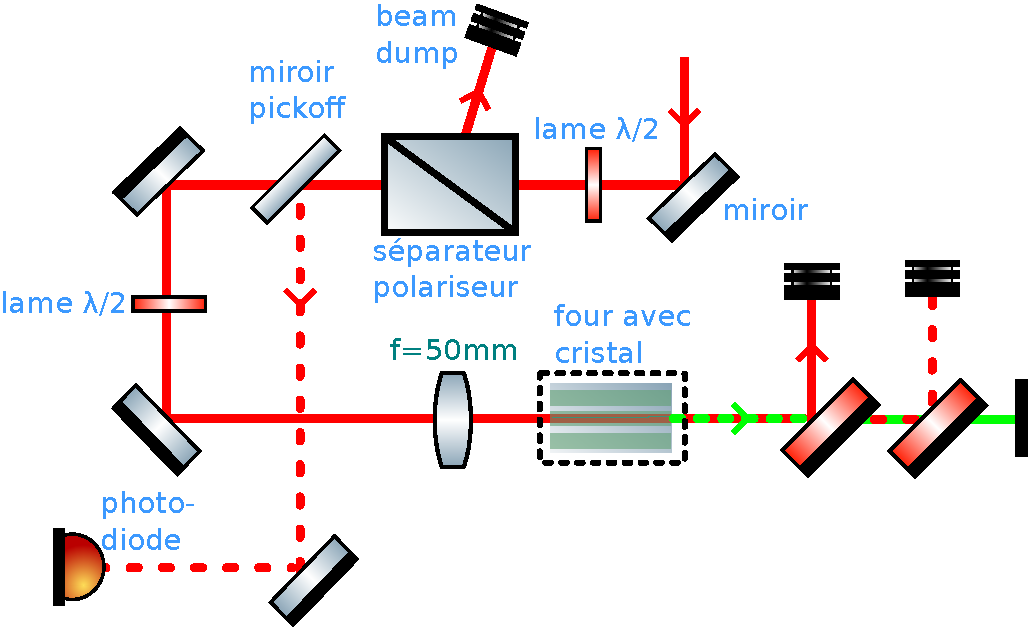
\includegraphics[height=8cm]{./img/schema.pdf}
	%%LaTeX with PSTricks extensions
%%Creator: Inkscape 1.2.2 (b0a8486, 2022-12-01)
%%Please note this file requires PSTricks extensions
\psset{xunit=.5pt,yunit=.5pt,runit=.5pt}
\begin{pspicture}(793.7007874,1122.51968504)
{
\newrgbcolor{curcolor}{0 0 0}
\pscustom[linewidth=0,linecolor=curcolor]
{
\newpath
\moveto(481.04617256,824.42653456)
\lineto(409.7164014,824.42653456)
\lineto(409.7164014,780.34567284)
\lineto(481.04617256,780.34567284)
\lineto(486.88963919,780.34567284)
\lineto(486.88963919,824.42653456)
\closepath
}
}
{
\newrgbcolor{curcolor}{1 0 0}
\pscustom[linewidth=5.15486004,linecolor=curcolor,linestyle=dashed,dash=1.36389005 4.09168005]
{
\newpath
\moveto(120.0614022,706.45175433)
\lineto(244.45846677,706.45175433)
}
}
{
\newrgbcolor{curcolor}{1 0 0}
\pscustom[linewidth=5.15486004,linecolor=curcolor]
{
\newpath
\moveto(494.93446299,1043.52720756)
\lineto(494.93446299,1097.75182413)
}
}
{
\newrgbcolor{curcolor}{1 0 0}
\pscustom[linewidth=5.15486004,linecolor=curcolor]
{
\newpath
\moveto(495.47285669,1030.41186898)
\lineto(495.47285669,951.80242016)
}
}
{
\newrgbcolor{curcolor}{1 0 0}
\pscustom[linewidth=5.15486004,linecolor=curcolor]
{
\newpath
\moveto(577.10211024,877.6012989)
\lineto(577.10211024,798.99183496)
}
}
{
\newrgbcolor{curcolor}{1 0 0}
\pscustom[linewidth=5.15486004,linecolor=curcolor,linestyle=dashed,dash=1.36389005 4.09168005]
{
\newpath
\moveto(654.13107402,879.39494929)
\lineto(654.13107402,800.78548535)
}
}
{
\newrgbcolor{curcolor}{1 0 0}
\pscustom[linewidth=5.15486004,linecolor=curcolor,linestyle=dashed,dash=1.36389005 4.09168005]
{
\newpath
\moveto(249.46311307,957.86754142)
\lineto(249.46311307,701.73977953)
}
}
{
\newrgbcolor{curcolor}{0 1 0}
\pscustom[linestyle=none,fillstyle=solid,fillcolor=curcolor]
{
\newpath
\moveto(598.18045984,801.48394205)
\lineto(707.27142047,801.48394205)
}
}
{
\newrgbcolor{curcolor}{0 1 0.01176471}
\pscustom[linewidth=5.15486004,linecolor=curcolor]
{
\newpath
\moveto(598.18045984,801.48394205)
\lineto(707.27142047,801.48394205)
}
}
{
\newrgbcolor{curcolor}{1 0 0}
\pscustom[linewidth=5.15486004,linecolor=curcolor,linestyle=dashed,dash=1.36389005 4.09168005]
{
\newpath
\moveto(643.00195276,801.39240189)
\lineto(600.92840315,801.39240189)
}
}
{
\newrgbcolor{curcolor}{1 0 0}
\pscustom[linewidth=5.15486004,linecolor=curcolor]
{
\newpath
\moveto(167.86343433,951.39717921)
\lineto(491.17700787,951.39717921)
}
}
{
\newrgbcolor{curcolor}{1 0 0}
\pscustom[linewidth=5.15486004,linecolor=curcolor]
{
\newpath
\moveto(342.90952819,942.48478866)
\lineto(372.07640693,1038.48422173)
}
}
{
\newrgbcolor{curcolor}{1 0 0}
\pscustom[linewidth=5.15486004,linecolor=curcolor]
{
\newpath
\moveto(164.03092913,802.17283654)
\lineto(571.41807874,802.17283654)
}
}
{
\newrgbcolor{curcolor}{0 0 0}
\pscustom[linewidth=1.55582199,linecolor=curcolor]
{
\newpath
\moveto(271.56784252,726.71496664)
\lineto(285.88115782,711.91918516)
\lineto(244.98555611,669.64509467)
\lineto(230.67224081,684.44087615)
\closepath
}
}
{
\newrgbcolor{curcolor}{0 0 0}
\pscustom[linestyle=none,fillstyle=solid,fillcolor=curcolor]
{
\newpath
\moveto(281.78957867,716.14868125)
\lineto(285.88115851,711.91918445)
\lineto(244.9855568,669.64509396)
\lineto(240.89397696,673.87459076)
\closepath
}
}
{
\newrgbcolor{curcolor}{0 0 0}
\pscustom[linewidth=1.55582199,linecolor=curcolor]
{
\newpath
\moveto(281.78957867,716.14868125)
\lineto(285.88115851,711.91918445)
\lineto(244.9855568,669.64509396)
\lineto(240.89397696,673.87459076)
\closepath
}
}
{
\newrgbcolor{curcolor}{0 0 0}
\pscustom[linewidth=2.21295946,linecolor=curcolor]
{
\newpath
\moveto(462.71419231,1054.11663288)
\lineto(462.71419231,1037.11303217)
\lineto(528.52526228,1037.11303217)
\lineto(528.52526228,1054.11663288)
\closepath
}
}
{
\newrgbcolor{curcolor}{0 0 0}
\pscustom[linewidth=2.21295946,linecolor=curcolor]
{
\newpath
\moveto(470.93876255,1037.11003103)
\lineto(470.93876255,1020.10643032)
\lineto(520.30069481,1020.10643032)
\lineto(520.30069481,1037.11003103)
\closepath
}
}
{
\newrgbcolor{curcolor}{0 0 0}
\pscustom[linewidth=2.21295946,linecolor=curcolor]
{
\newpath
\moveto(487.39370542,1071.11723245)
\lineto(487.39370542,1054.11363174)
\lineto(503.84574778,1054.11363174)
\lineto(503.84574778,1071.11723245)
\closepath
}
}
{
\newrgbcolor{curcolor}{0 0 0}
\pscustom[linewidth=1.34271185,linecolor=curcolor]
{
\newpath
\moveto(265.02399753,983.17442162)
\lineto(274.76085509,973.43756406)
\lineto(228.48038354,927.15709251)
\lineto(218.74352598,936.89395007)
\closepath
}
}
{
\newrgbcolor{curcolor}{1 0 0}
\pscustom[linewidth=5.15486004,linecolor=curcolor]
{
\newpath
\moveto(164.31138898,948.39497575)
\lineto(164.31138898,804.04807559)
}
}
{
\newrgbcolor{curcolor}{0 0 0}
\pscustom[linewidth=1.55582199,linecolor=curcolor]
{
\newpath
\moveto(187.46274995,973.34351622)
\lineto(172.66696847,987.65683153)
\lineto(130.39287798,946.76122981)
\lineto(145.18865946,932.44791451)
\closepath
}
}
{
\newrgbcolor{curcolor}{0 0 0}
\pscustom[linestyle=none,fillstyle=solid,fillcolor=curcolor]
{
\newpath
\moveto(176.89646456,983.56525237)
\lineto(172.66696776,987.65683221)
\lineto(130.39287727,946.7612305)
\lineto(134.62237407,942.66965066)
\closepath
}
}
{
\newrgbcolor{curcolor}{0 0 0}
\pscustom[linewidth=1.55582199,linecolor=curcolor]
{
\newpath
\moveto(176.89646456,983.56525237)
\lineto(172.66696776,987.65683221)
\lineto(130.39287727,946.7612305)
\lineto(134.62237407,942.66965066)
\closepath
}
}
{
\newrgbcolor{curcolor}{0 0 0}
\pscustom[linewidth=1.55582199,linecolor=curcolor]
{
\newpath
\moveto(144.30504945,823.26191341)
\lineto(129.99173414,808.46613193)
\lineto(170.88733586,766.19204144)
\lineto(185.20065116,780.98782292)
\closepath
}
}
{
\newrgbcolor{curcolor}{0 0 0}
\pscustom[linestyle=none,fillstyle=solid,fillcolor=curcolor]
{
\newpath
\moveto(134.0833133,812.69562803)
\lineto(129.99173346,808.46613122)
\lineto(170.88733517,766.19204073)
\lineto(174.97891501,770.42153754)
\closepath
}
}
{
\newrgbcolor{curcolor}{0 0 0}
\pscustom[linewidth=1.55582199,linecolor=curcolor]
{
\newpath
\moveto(134.0833133,812.69562803)
\lineto(129.99173346,808.46613122)
\lineto(170.88733517,766.19204073)
\lineto(174.97891501,770.42153754)
\closepath
}
}
{
\newrgbcolor{curcolor}{0 0 0}
\pscustom[linewidth=1.55582199,linecolor=curcolor]
{
\newpath
\moveto(188.87357969,870.88278205)
\lineto(188.87357969,879.85068139)
\lineto(142.60304234,879.85068139)
\lineto(142.60304234,870.88278205)
\closepath
}
}
{
\newrgbcolor{curcolor}{0 0 0}
\pscustom[linewidth=2.00976889,linecolor=curcolor]
{
\newpath
\moveto(354.17527824,830.89080241)
\lineto(340.31857065,830.89080241)
\curveto(337.49873338,824.07767415)(335.66243356,813.24519556)(335.66243356,801.00528545)
\curveto(335.66243356,788.76537534)(337.49873338,777.93289675)(340.31857065,771.12240413)
\lineto(354.17527824,771.12240413)
\curveto(357.00056447,777.93289675)(358.83141533,788.76537534)(358.83141533,801.00528545)
\curveto(358.83141533,813.24519556)(356.99511551,824.07767415)(354.17527824,830.89080241)
\closepath
}
}
{
\newrgbcolor{curcolor}{0 0 0}
\pscustom[linewidth=3.80579535,linecolor=curcolor]
{
\newpath
\moveto(303.3273003,982.38098145)
\lineto(387.37600492,982.38098145)
\lineto(387.37600492,920.84456797)
\lineto(303.3273003,920.84456797)
\closepath
}
}
{
\newrgbcolor{curcolor}{0 0 0}
\pscustom[linewidth=3.818419,linecolor=curcolor]
{
\newpath
\moveto(303.25676865,982.44545764)
\lineto(387.68641194,920.77997643)
}
}
{
\newrgbcolor{curcolor}{0 0 0}
\pscustom[linewidth=0.77791099,linecolor=curcolor]
{
\newpath
\moveto(367.10854123,1064.35028585)
\lineto(360.3175804,1045.69227224)
\lineto(383.74570412,1037.1651325)
\lineto(390.53666495,1055.82314611)
\closepath
}
}
{
\newrgbcolor{curcolor}{0 0 0}
\pscustom[linestyle=none,fillstyle=solid,fillcolor=curcolor]
{
\newpath
\moveto(363.08266641,1066.55055969)
\lineto(362.18595113,1064.08685443)
\lineto(394.02627975,1052.49792248)
\lineto(394.92299502,1054.96162773)
\closepath
}
}
{
\newrgbcolor{curcolor}{0 0 0}
\pscustom[linewidth=1.03721466,linecolor=curcolor]
{
\newpath
\moveto(363.08266641,1066.55055969)
\lineto(362.18595113,1064.08685443)
\lineto(394.02627975,1052.49792248)
\lineto(394.92299502,1054.96162773)
\closepath
}
}
{
\newrgbcolor{curcolor}{0 0 0}
\pscustom[linestyle=none,fillstyle=solid,fillcolor=curcolor]
{
\newpath
\moveto(360.88972652,1060.52550616)
\lineto(359.5586102,1056.86829374)
\lineto(391.39893881,1045.27936179)
\lineto(392.73005513,1048.93657421)
\closepath
}
}
{
\newrgbcolor{curcolor}{0 0 0}
\pscustom[linewidth=1.03721466,linecolor=curcolor]
{
\newpath
\moveto(360.88972652,1060.52550616)
\lineto(359.5586102,1056.86829374)
\lineto(391.39893881,1045.27936179)
\lineto(392.73005513,1048.93657421)
\closepath
}
}
{
\newrgbcolor{curcolor}{0 0 0}
\pscustom[linestyle=none,fillstyle=solid,fillcolor=curcolor]
{
\newpath
\moveto(358.3004173,1053.41143677)
\lineto(355.64516299,1046.11618471)
\lineto(387.48549161,1034.52725276)
\lineto(390.14074591,1041.82250482)
\closepath
}
}
{
\newrgbcolor{curcolor}{0 0 0}
\pscustom[linewidth=1.03721466,linecolor=curcolor]
{
\newpath
\moveto(358.3004173,1053.41143677)
\lineto(355.64516299,1046.11618471)
\lineto(387.48549161,1034.52725276)
\lineto(390.14074591,1041.82250482)
\closepath
}
}
{
\newrgbcolor{curcolor}{0 0 0}
\pscustom[linewidth=1.55582199,linecolor=curcolor]
{
\newpath
\moveto(432.92965953,928.32353653)
\lineto(441.89755888,928.32353653)
\lineto(441.89755888,974.59407388)
\lineto(432.92965953,974.59407388)
\closepath
}
}
{
\newrgbcolor{curcolor}{0 0 0}
\pscustom[linewidth=1.55582199,linecolor=curcolor]
{
\newpath
\moveto(472.62369163,930.19138016)
\lineto(487.4194731,915.87806485)
\lineto(529.69356359,956.77366656)
\lineto(514.89778212,971.08698187)
\closepath
}
}
{
\newrgbcolor{curcolor}{0 0 0}
\pscustom[linestyle=none,fillstyle=solid,fillcolor=curcolor]
{
\newpath
\moveto(483.18997701,919.96964401)
\lineto(487.41947382,915.87806416)
\lineto(529.69356431,956.77366588)
\lineto(525.4640675,960.86524572)
\closepath
}
}
{
\newrgbcolor{curcolor}{0 0 0}
\pscustom[linewidth=1.55582199,linecolor=curcolor]
{
\newpath
\moveto(483.18997701,919.96964401)
\lineto(487.41947382,915.87806416)
\lineto(529.69356431,956.77366588)
\lineto(525.4640675,960.86524572)
\closepath
}
}
{
\newrgbcolor{curcolor}{0 0 0}
\pscustom[linewidth=1.72786126,linecolor=curcolor]
{
\newpath
\moveto(672.12706254,826.58292406)
\lineto(688.55892777,810.15105883)
\lineto(643.14118242,764.73331348)
\lineto(626.70931719,781.16517871)
\closepath
}
}
{
\newrgbcolor{curcolor}{0 0 0}
\pscustom[linestyle=none,fillstyle=solid,fillcolor=curcolor]
{
\newpath
\moveto(683.86174365,814.84824295)
\lineto(688.55892856,810.15105804)
\lineto(643.14118321,764.73331269)
\lineto(638.4439983,769.4304976)
\closepath
}
}
{
\newrgbcolor{curcolor}{0 0 0}
\pscustom[linewidth=1.72786126,linecolor=curcolor]
{
\newpath
\moveto(683.86174365,814.84824295)
\lineto(688.55892856,810.15105804)
\lineto(643.14118321,764.73331269)
\lineto(638.4439983,769.4304976)
\closepath
}
}
{
\newrgbcolor{curcolor}{0 0 0}
\pscustom[linestyle=none,fillstyle=solid,fillcolor=curcolor]
{
\newpath
\moveto(708.28488327,822.25878137)
\lineto(714.4281542,822.25878137)
\lineto(714.4281542,774.72147664)
\lineto(708.28488327,774.72147664)
\closepath
}
}
{
\newrgbcolor{curcolor}{0 0 0}
\pscustom[linewidth=1.59849069,linecolor=curcolor]
{
\newpath
\moveto(708.28488327,822.25878137)
\lineto(714.4281542,822.25878137)
\lineto(714.4281542,774.72147664)
\lineto(708.28488327,774.72147664)
\closepath
}
}
{
\newrgbcolor{curcolor}{0 0 0}
\pscustom[linewidth=0.77791103,linecolor=curcolor]
{
\newpath
\moveto(564.59961652,899.80578202)
\lineto(564.59961652,879.95033824)
\lineto(589.53130622,879.95033824)
\lineto(589.53130622,899.80578202)
\closepath
}
}
{
\newrgbcolor{curcolor}{0 0 0}
\pscustom[linestyle=none,fillstyle=solid,fillcolor=curcolor]
{
\newpath
\moveto(560.0639935,900.49643284)
\lineto(560.0639935,897.87461241)
\lineto(593.94776509,897.87461241)
\lineto(593.94776509,900.49643284)
\closepath
}
}
{
\newrgbcolor{curcolor}{0 0 0}
\pscustom[linewidth=1.0372147,linecolor=curcolor]
{
\newpath
\moveto(560.0639935,900.49643284)
\lineto(560.0639935,897.87461241)
\lineto(593.94776509,897.87461241)
\lineto(593.94776509,900.49643284)
\closepath
}
}
{
\newrgbcolor{curcolor}{0 0 0}
\pscustom[linestyle=none,fillstyle=solid,fillcolor=curcolor]
{
\newpath
\moveto(560.0639935,894.08470467)
\lineto(560.0639935,890.19278042)
\lineto(593.94776509,890.19278042)
\lineto(593.94776509,894.08470467)
\closepath
}
}
{
\newrgbcolor{curcolor}{0 0 0}
\pscustom[linewidth=1.0372147,linecolor=curcolor]
{
\newpath
\moveto(560.0639935,894.08470467)
\lineto(560.0639935,890.19278042)
\lineto(593.94776509,890.19278042)
\lineto(593.94776509,894.08470467)
\closepath
}
}
{
\newrgbcolor{curcolor}{0 0 0}
\pscustom[linestyle=none,fillstyle=solid,fillcolor=curcolor]
{
\newpath
\moveto(560.0639935,886.51406999)
\lineto(560.0639935,878.75062473)
\lineto(593.94776509,878.75062473)
\lineto(593.94776509,886.51406999)
\closepath
}
}
{
\newrgbcolor{curcolor}{0 0 0}
\pscustom[linewidth=1.0372147,linecolor=curcolor]
{
\newpath
\moveto(560.0639935,886.51406999)
\lineto(560.0639935,878.75062473)
\lineto(593.94776509,878.75062473)
\lineto(593.94776509,886.51406999)
\closepath
}
}
{
\newrgbcolor{curcolor}{0 0 0}
\pscustom[linewidth=0.77791103,linecolor=curcolor]
{
\newpath
\moveto(641.75171731,901.91199935)
\lineto(641.75171731,882.05655556)
\lineto(666.68340701,882.05655556)
\lineto(666.68340701,901.91199935)
\closepath
}
}
{
\newrgbcolor{curcolor}{0 0 0}
\pscustom[linestyle=none,fillstyle=solid,fillcolor=curcolor]
{
\newpath
\moveto(637.21609429,902.60265016)
\lineto(637.21609429,899.98082974)
\lineto(671.09986588,899.98082974)
\lineto(671.09986588,902.60265016)
\closepath
}
}
{
\newrgbcolor{curcolor}{0 0 0}
\pscustom[linewidth=1.0372147,linecolor=curcolor]
{
\newpath
\moveto(637.21609429,902.60265016)
\lineto(637.21609429,899.98082974)
\lineto(671.09986588,899.98082974)
\lineto(671.09986588,902.60265016)
\closepath
}
}
{
\newrgbcolor{curcolor}{0 0 0}
\pscustom[linestyle=none,fillstyle=solid,fillcolor=curcolor]
{
\newpath
\moveto(637.21609429,896.19092199)
\lineto(637.21609429,892.29899774)
\lineto(671.09986588,892.29899774)
\lineto(671.09986588,896.19092199)
\closepath
}
}
{
\newrgbcolor{curcolor}{0 0 0}
\pscustom[linewidth=1.0372147,linecolor=curcolor]
{
\newpath
\moveto(637.21609429,896.19092199)
\lineto(637.21609429,892.29899774)
\lineto(671.09986588,892.29899774)
\lineto(671.09986588,896.19092199)
\closepath
}
}
{
\newrgbcolor{curcolor}{0 0 0}
\pscustom[linestyle=none,fillstyle=solid,fillcolor=curcolor]
{
\newpath
\moveto(637.21609429,888.62028731)
\lineto(637.21609429,880.85684206)
\lineto(671.09986588,880.85684206)
\lineto(671.09986588,888.62028731)
\closepath
}
}
{
\newrgbcolor{curcolor}{0 0 0}
\pscustom[linewidth=1.0372147,linecolor=curcolor]
{
\newpath
\moveto(637.21609429,888.62028731)
\lineto(637.21609429,880.85684206)
\lineto(671.09986588,880.85684206)
\lineto(671.09986588,888.62028731)
\closepath
}
}
{
\newrgbcolor{curcolor}{0 0 0}
\pscustom[linewidth=1.55582199,linecolor=curcolor]
{
\newpath
\moveto(103.77247789,686.14119811)
\curveto(101.76071535,686.14119811)(99.82240459,686.45334513)(97.98815051,687.02069344)
\lineto(97.98815051,727.1147133)
\curveto(99.82240459,727.67995251)(101.76071535,727.99209953)(103.77247789,727.99209953)
\curveto(114.95143017,727.99209953)(124.01456323,718.62557969)(124.01456323,707.06770337)
\curveto(124.01456323,695.50982705)(114.95143017,686.14119811)(103.77247789,686.14119811)
\closepath
}
}
{
\newrgbcolor{curcolor}{0 0 0}
\pscustom[linestyle=none,fillstyle=solid,fillcolor=curcolor]
{
\newpath
\moveto(92.20586346,683.15260126)
\lineto(97.99019091,683.15260126)
\lineto(97.99019091,730.98280442)
\lineto(92.20586346,730.98280442)
\closepath
}
}
{
\newrgbcolor{curcolor}{0 0 0}
\pscustom[linewidth=1.55582199,linecolor=curcolor]
{
\newpath
\moveto(92.20586346,683.15260126)
\lineto(97.99019091,683.15260126)
\lineto(97.99019091,730.98280442)
\lineto(92.20586346,730.98280442)
\closepath
}
}
{
\newrgbcolor{curcolor}{0 0.50196081 0.50196081}
\pscustom[linestyle=none,fillstyle=solid,fillcolor=curcolor]
{
\newpath
\moveto(320.27327762,861.60655507)
\lineto(320.27327762,859.73852447)
\lineto(318.12443197,859.73852447)
\curveto(317.31861485,859.73852447)(316.75698473,859.57573314)(316.43954162,859.25015046)
\curveto(316.13023808,858.92456779)(315.97558631,858.33851897)(315.97558631,857.49200402)
\lineto(315.97558631,856.28327833)
\lineto(319.67501946,856.28327833)
\lineto(319.67501946,854.53734124)
\lineto(315.97558631,854.53734124)
\lineto(315.97558631,842.60880598)
\lineto(313.7168565,842.60880598)
\lineto(313.7168565,854.53734124)
\lineto(311.56801085,854.53734124)
\lineto(311.56801085,856.28327833)
\lineto(313.7168565,856.28327833)
\lineto(313.7168565,857.23560766)
\curveto(313.7168565,858.75770666)(314.07092766,859.86468776)(314.77906998,860.55655094)
\curveto(315.4872123,861.2565537)(316.61047253,861.60655507)(318.14885067,861.60655507)
\closepath
}
}
{
\newrgbcolor{curcolor}{0 0.50196081 0.50196081}
\pscustom[linestyle=none,fillstyle=solid,fillcolor=curcolor]
{
\newpath
\moveto(322.44654179,853.96350177)
\lineto(338.0989289,853.96350177)
\lineto(338.0989289,851.91233092)
\lineto(322.44654179,851.91233092)
\closepath
\moveto(322.44654179,848.98208684)
\lineto(338.0989289,848.98208684)
\lineto(338.0989289,846.90649729)
\lineto(322.44654179,846.90649729)
\closepath
}
}
{
\newrgbcolor{curcolor}{0 0.50196081 0.50196081}
\pscustom[linestyle=none,fillstyle=solid,fillcolor=curcolor]
{
\newpath
\moveto(343.44662412,860.837366)
\lineto(353.12863892,860.837366)
\lineto(353.12863892,858.76177645)
\lineto(345.70535393,858.76177645)
\lineto(345.70535393,854.29315423)
\curveto(346.06349487,854.41524774)(346.42163581,854.50478297)(346.77977675,854.56175994)
\curveto(347.1379177,854.62687647)(347.49605864,854.65943474)(347.85419958,854.65943474)
\curveto(349.8890913,854.65943474)(351.50072554,854.10187441)(352.68910231,852.98675375)
\curveto(353.87747907,851.87163309)(354.47166745,850.36174343)(354.47166745,848.45708478)
\curveto(354.47166745,846.49544916)(353.86119994,844.96928037)(352.64026491,843.87857841)
\curveto(351.41932987,842.79601602)(349.69781148,842.25473482)(347.47570972,842.25473482)
\curveto(346.71059044,842.25473482)(345.92919202,842.31985136)(345.13151446,842.45008443)
\curveto(344.34197647,842.5803175)(343.52395,842.7756671)(342.67743505,843.03613324)
\lineto(342.67743505,845.51463135)
\curveto(343.40999607,845.11579258)(344.16697579,844.81869839)(344.94837421,844.62334878)
\curveto(345.72977263,844.42799918)(346.55593866,844.33032437)(347.42687232,844.33032437)
\curveto(348.83501739,844.33032437)(349.95013805,844.70067467)(350.77223431,845.44137525)
\curveto(351.59433056,846.18207584)(352.00537869,847.18731235)(352.00537869,848.45708478)
\curveto(352.00537869,849.72685721)(351.59433056,850.73209372)(350.77223431,851.47279431)
\curveto(349.95013805,852.2134949)(348.83501739,852.58384519)(347.42687232,852.58384519)
\curveto(346.7675674,852.58384519)(346.10826249,852.51058909)(345.44895757,852.36407688)
\curveto(344.79779222,852.21756468)(344.13034774,851.98965681)(343.44662412,851.68035326)
\closepath
}
}
{
\newrgbcolor{curcolor}{0 0.50196081 0.50196081}
\pscustom[linestyle=none,fillstyle=solid,fillcolor=curcolor]
{
\newpath
\moveto(368.85428391,855.75827627)
\lineto(368.85428391,853.65826802)
\curveto(368.21939769,854.00826939)(367.58044169,854.26873553)(366.93741591,854.43966644)
\curveto(366.30252969,854.61873691)(365.65950391,854.70827214)(365.00833856,854.70827214)
\curveto(363.55135608,854.70827214)(362.41995629,854.24431683)(361.61413917,853.31640621)
\curveto(360.80832205,852.39663515)(360.40541349,851.10244402)(360.40541349,849.43383281)
\curveto(360.40541349,847.7652216)(360.80832205,846.46696068)(361.61413917,845.53905006)
\curveto(362.41995629,844.619279)(363.55135608,844.15939347)(365.00833856,844.15939347)
\curveto(365.65950391,844.15939347)(366.30252969,844.24485892)(366.93741591,844.41578983)
\curveto(367.58044169,844.5948603)(368.21939769,844.85939622)(368.85428391,845.2093976)
\lineto(368.85428391,843.13380804)
\curveto(368.22753726,842.84078364)(367.57637191,842.62101533)(366.90078786,842.47450313)
\curveto(366.23334337,842.32799092)(365.52113127,842.25473482)(364.76415155,842.25473482)
\curveto(362.70484113,842.25473482)(361.06878819,842.90183039)(359.85599272,844.19602152)
\curveto(358.64319726,845.49021265)(358.03679953,847.23614975)(358.03679953,849.43383281)
\curveto(358.03679953,851.66407413)(358.64726704,853.41815079)(359.86820207,854.69606279)
\curveto(361.09727667,855.97397479)(362.77809723,856.61293079)(364.91066375,856.61293079)
\curveto(365.60252694,856.61293079)(366.27811099,856.53967469)(366.93741591,856.39316249)
\curveto(367.59672082,856.25478985)(368.23567682,856.04316111)(368.85428391,855.75827627)
\closepath
}
}
{
\newrgbcolor{curcolor}{0 0.50196081 0.50196081}
\pscustom[linestyle=none,fillstyle=solid,fillcolor=curcolor]
{
\newpath
\moveto(383.40782903,853.65826802)
\curveto(383.96945914,854.66757431)(384.64097341,855.41234468)(385.42237183,855.89257912)
\curveto(386.20377025,856.37281357)(387.12354131,856.61293079)(388.181685,856.61293079)
\curveto(389.60610921,856.61293079)(390.70495073,856.11234743)(391.47820959,855.1111807)
\curveto(392.25146844,854.11815354)(392.63809787,852.70186891)(392.63809787,850.86232679)
\lineto(392.63809787,842.60880598)
\lineto(390.37936806,842.60880598)
\lineto(390.37936806,850.78907069)
\curveto(390.37936806,852.09954096)(390.1473904,853.0722192)(389.68343509,853.70710542)
\curveto(389.21947978,854.34199163)(388.51133746,854.65943474)(387.55900814,854.65943474)
\curveto(386.39505007,854.65943474)(385.47527902,854.27280532)(384.79969497,853.49954646)
\curveto(384.12411091,852.72628761)(383.78631889,851.6722137)(383.78631889,850.33732473)
\lineto(383.78631889,842.60880598)
\lineto(381.52758908,842.60880598)
\lineto(381.52758908,850.78907069)
\curveto(381.52758908,852.10768053)(381.29561142,853.08035877)(380.83165611,853.70710542)
\curveto(380.3677008,854.34199163)(379.65141891,854.65943474)(378.68281046,854.65943474)
\curveto(377.53513153,854.65943474)(376.62350004,854.26873553)(375.94791599,853.48733711)
\curveto(375.27233193,852.71407826)(374.93453991,851.66407413)(374.93453991,850.33732473)
\lineto(374.93453991,842.60880598)
\lineto(372.6758101,842.60880598)
\lineto(372.6758101,856.28327833)
\lineto(374.93453991,856.28327833)
\lineto(374.93453991,854.15885138)
\curveto(375.44733262,854.99722677)(376.06186992,855.61583385)(376.77815181,856.01467263)
\curveto(377.49443369,856.4135114)(378.34501843,856.61293079)(379.32990602,856.61293079)
\curveto(380.32293318,856.61293079)(381.16537835,856.36060422)(381.85724154,855.85595107)
\curveto(382.55724429,855.35129793)(383.07410679,854.61873691)(383.40782903,853.65826802)
\closepath
}
}
{
\newrgbcolor{curcolor}{0 0.50196081 0.50196081}
\pscustom[linestyle=none,fillstyle=solid,fillcolor=curcolor]
{
\newpath
\moveto(410.84288504,802.56537827)
\lineto(486.19653543,803.0067515)
}
}
{
\newrgbcolor{curcolor}{0.60000002 0.60000002 0.60000002}
\pscustom[linestyle=none,fillstyle=solid,fillcolor=curcolor]
{
\newpath
\moveto(482.16185197,802.00899402)
\lineto(414.66908976,802.00899402)
}
}
{
\newrgbcolor{curcolor}{0.3764706 0.62352943 0.4509804}
\pscustom[linewidth=9.41665469,linecolor=curcolor,strokeopacity=0.59946299]
{
\newpath
\moveto(482.16185197,802.00899402)
\lineto(414.66908976,802.00899402)
}
}
{
\newrgbcolor{curcolor}{0.60000002 0.60000002 0.60000002}
\pscustom[linestyle=none,fillstyle=solid,fillcolor=curcolor]
{
\newpath
\moveto(481.87101732,814.91112945)
\lineto(414.37829291,814.91112945)
}
}
{
\newrgbcolor{curcolor}{0.3764706 0.62352943 0.4509804}
\pscustom[linewidth=9.41665469,linecolor=curcolor,strokeopacity=0.59946299]
{
\newpath
\moveto(481.87101732,814.91112945)
\lineto(414.37829291,814.91112945)
}
}
{
\newrgbcolor{curcolor}{0.60000002 0.60000002 0.60000002}
\pscustom[linestyle=none,fillstyle=solid,fillcolor=curcolor]
{
\newpath
\moveto(482.1112063,787.65752315)
\lineto(414.61851969,787.65752315)
}
}
{
\newrgbcolor{curcolor}{0.3764706 0.62352943 0.4509804}
\pscustom[linewidth=9.41665469,linecolor=curcolor,strokeopacity=0.59946299]
{
\newpath
\moveto(482.1112063,787.65752315)
\lineto(414.61851969,787.65752315)
}
}
{
\newrgbcolor{curcolor}{0 1 0}
\pscustom[linestyle=none,fillstyle=solid,fillcolor=curcolor]
{
\newpath
\moveto(488.47181102,801.94171843)
\lineto(597.56277165,801.94171843)
}
}
{
\newrgbcolor{curcolor}{0 1 0.01176471}
\pscustom[linewidth=5.15486004,linecolor=curcolor,linestyle=dashed,dash=1.36389005 2.7277801]
{
\newpath
\moveto(488.47181102,801.94171843)
\lineto(597.56277165,801.94171843)
}
}
{
\newrgbcolor{curcolor}{0 0 0}
\pscustom[linewidth=3.38783617,linecolor=curcolor,linestyle=dashed,dash=0.89636499 1.79273999]
{
\newpath
\moveto(404.14821445,830.99617064)
\lineto(494.53787406,830.99617064)
\curveto(495.22933885,830.99617064)(495.78600546,830.43950404)(495.78600546,829.74803925)
\lineto(495.78600546,774.95494422)
\curveto(495.78600546,774.26347943)(495.22933885,773.70681282)(494.53787406,773.70681282)
\lineto(404.14821445,773.70681282)
\curveto(403.45674965,773.70681282)(402.90008305,774.26347943)(402.90008305,774.95494422)
\lineto(402.90008305,829.74803925)
\curveto(402.90008305,830.43950404)(403.45674965,830.99617064)(404.14821445,830.99617064)
\closepath
}
}
{
\newrgbcolor{curcolor}{0 0 0}
\pscustom[linewidth=1.72786126,linecolor=curcolor]
{
\newpath
\moveto(603.37042632,827.14380595)
\lineto(619.80229155,810.71194072)
\lineto(574.3845462,765.29419537)
\lineto(557.95268097,781.7260606)
\closepath
}
}
{
\newrgbcolor{curcolor}{0 0 0}
\pscustom[linestyle=none,fillstyle=solid,fillcolor=curcolor]
{
\newpath
\moveto(615.10510743,815.40912484)
\lineto(619.80229234,810.71193993)
\lineto(574.38454699,765.29419458)
\lineto(569.68736208,769.99137949)
\closepath
}
}
{
\newrgbcolor{curcolor}{0 0 0}
\pscustom[linewidth=1.72786126,linecolor=curcolor]
{
\newpath
\moveto(615.10510743,815.40912484)
\lineto(619.80229234,810.71193993)
\lineto(574.38454699,765.29419458)
\lineto(569.68736208,769.99137949)
\closepath
}
}
\end{pspicture}

	\caption{Schéma du montage}
	\label{fig:montage}
\end{figure}

De façon plus détaillée, l'ajustement se fait ensuite selon le protocole suivant :
\begin{enumerate}
	\item À l'aide des quatre vis des deux miroirs, on cherche à obtenir un faisceau le plus horizontal possible à la hauteur du cristal, d'abord sans puis avec lentille. La procédure est analogue à celle pour coupler la fibre.
	\item On place ensuite le cristal au point focal de la lentille et on le translate transversalement (à l'aide d'une platine de translation) jusqu'à faire passer le faisceau par la bande avec la période d'inversion choisie.
	\item On tourne la lame demi-onde devant le cristal afin d'aligner la direction de polarisation (linéaire) avec l'axe extraordinaire du cristal.
	\item On se place à une température élevée que l'on laisse décroître et on attend de voir apparaître le pic principal.
	\item Lorsque l'alignement n'est pas bon, le pic principal et les pics secondaires sont d'amplitudes comparables et il est difficile de trouver la température optimale. Il s'agit donc d'alterner optimisation de l'alignement et de la température.
	\item Une fois dépassé quelques dizaines de $\unit{\micro\watt}$ de vert, on peut passer d'une estimation de la puissance à l'\oe il à une mesure au puissance-mètre.
	\item On fait une dernière recherche fine d'optimum de température (en variant par pas de $\SI{0.2}{\celsius}$ sur une plage de $\SI{1}{\celsius}$).
	\item On optimise finement l'alignement. %On note que changer un seul angle influence très fortement la puissance de vert produite, mais que la variation de l'angle correspondant sur le deuxième miroir permet de retrouver une puissance optimale semblable. Il faut donc `beam-walker' considérablement afin de trouver le véritable optimum. De plus, il y a une certaine compensation entre alignement (et donc $\Lambda$ effective pour l'angle du faisceau) et température (et donc $\Delta k$, mais aussi $\Lambda$ à travers la dilatation thermique).
\end{enumerate}





% Il faut noter que en pratique, on commence par choisir un waist et donc fixer un $a$, et on cherche ensuite à optimiser $b$ en ajustant la température et l'alignement.



%\begin{figure}[h]
%    \centering
%    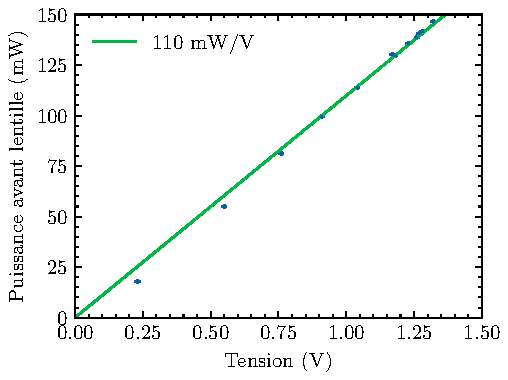
\includegraphics{../donnees/calib photodiode.pdf}
%    \caption{Calibration de la photodiode (après glan)}
%\end{figure}



Le régime de doublage trouvé initialement a été pour la bande avec $\Lambda = \SI{6.9}{\micro\meter}$ et une température optimale autour de $\SI{83}{\celsius}$.

\section{Étude à basse puissance}

L'étude du doublage est d'abord faite à basse puissance afin d'éviter les effets thermiques qui, comme nous le verrons, compliquent considérablement le comportement à haute puissance. À haute puissance comme à basse puissance, l'accord avec la théorie laisse à désirer et, au vu du temps limité à disposition pour étudier la question, on doit se contenter des hypothèses pour expliquer le comportement observé.

\subsection{Efficactité de conversion}

On vérifie tout d'abord que la puissance générée est bien quadratique en la puissance incidente, comme en témoignent les données présentées figure \ref{fig:quadra}. On fait ensuite varier la température autour de l'optimum, en gardant les autres paramètres fixés. On obtient alors les mesures figure \ref{fig:alphabp}, qui montrent un optimum à $\SI{83.3}{\celsius}$ (on rappelle que l'on travaille avec la bande $\Lambda = \SI{6.9}{\micro\meter}$). L'allure de la courbe est plutôt en accord avec celle prédite par la théorie de Boyd et Kleinman. 

\begin{figure}[htpb]
\centering
\hspace*{-0.4cm}
\begin{subfigure}[b]{0.45\textwidth}
    \centering
    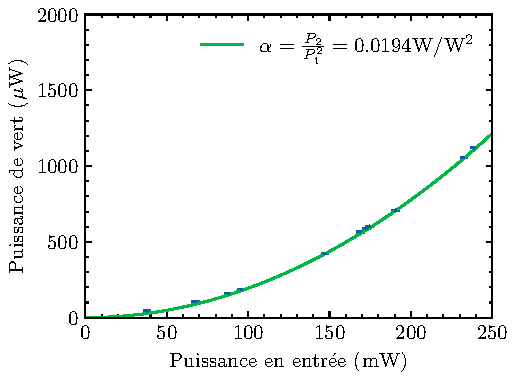
\includegraphics[height=6cm]{../donnees/conversion basse puissance 82.5 C.pdf}
    \caption{Vérification de la relation quadratique entre puissance incidente et doublée {(à~\SI{82.5}{\celsius})}}
    \label{fig:quadra}
\end{subfigure}
\hspace*{0.4cm}
\begin{subfigure}[b]{0.48\textwidth}
	\centering
	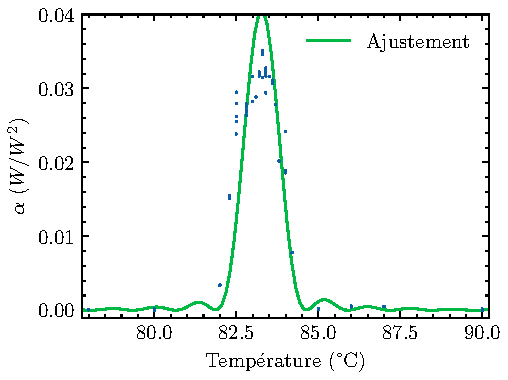
\includegraphics[height=6cm]{./img/alpha bp.pdf}
	\caption{Dépendance en température de l'efficacité de conversion}
	\label{fig:alphabp}
\end{subfigure}
\caption{Efficacité de conversion mesurée à basse puissance}
\end{figure}

En effet, le tracé de $\alpha$ en fonction de la température correspond, modulo la variation du préfacteur $\frac{\chie^2 L}{n_1 n_2}$, à la variation de $h(a,b)$ avec $a$ fixé et $b=-\Delta k_\mathsc{eff} \zr$ variant avec les indices optiques. Si on linéarise la variation d'indices optiques au voisinage de l'optimum de température, on a alors 
\begin{align}
	\delta b = - \zr \left[ 2\pi \left( \frac{\beta}{\Lambda} + \frac{1}{\lambda_2} \pdv{(n_2-n_1)}{T}  \right) + \frac{\dke}{n_1} \pdv{n_1}{T} \right] \delta T \approx -\left(0.3+5.5+\num{3e-4}\right) \delta T = - 5.8 \delta T
\end{align}
avec $\beta = \num{1.5e-5}$ le coefficient de dilatation thermique du cristal.
Les graphes de $\alpha(T)$ et de $h(a,b)$ à $a$ fixé (figure \ref{fig:bk-factor}) sont alors reliés par dilatation des deux axes.

L'accord quantitatif pose plus de difficultés. En effet, on ne peut se fier avec certitude ni à la valeur de température indiquée par le module de contrôle du four (dont la sonde est au niveau de la monture en cuivre et non à l'intérieur du cristal chauffé par le laser), qui indiquait d'ailleurs $\SI{30}{\celsius}$ laser et asservissement éteints dans une salle à $\SI{25}{\celsius}$, ni à la valeur exacte de la période d'inversion $\Lambda$ (qui varie d'ailleurs aussi avec la dilatation thermique). Il est donc difficile de se placer sur la courbe figure \ref{fig:lp}, or il est nécessaire de connaître la température du cristal au niveau du faisceau pour avoir une valeur exacte des indices optiques et de $\Lambda$ et ainsi pouvoir calculer $\dke$.
La valeur de $\chie$ varie d'un cristal à un autre et est également source d'incertitude. Covesion annonce d'ailleurs $\chie = \SI{28}{pm/V}$ alors que la valeur théorique correspondant à $\chi^{(2)}=\SI{50}{pm/V}$ est $\chie = \SI{32}{pm/V}$, ce qui fait passer le facteur devant $h$ de $\SI{5.5}{\percent\per\watt}$ à $\SI{4.2}{\percent\per\watt}$.

Encore une autre source d'incertitude est la détermination du waist du faisceau incident dont $\zr$ dépend quadratiquement. D'ailleurs, avec le waist déterminé à $\SI{62.6}{\micro\meter}$, $a=0.41$ ce qui correspond à un maximum de $h = 0.39$ et donc un maximum de seulement $\alphae{2.1}$ même pour $\chie = \SI{32}{pm/V}$. Il faudrait plutôt $a=0.7$, ce qui correspond à un waist $\sqrt2$ fois plus petit, ce qui est difficiement reconciliable avec les mesures effectuées. % puisque un des waists $w(z)$ mesurés vaut $\SI{68\pm10}{\micro m}$, ce qui impose une borne supérieure sur la valeur de $w_0$. 
Il est également difficile d'imaginer un $\chie=\SI{40}{pm/V}$ qui permettrait d'augmenter suffisamment le préfacteur de $h$. Cette efficacité plus grande que prévu est d'autant plus étonnante que les mesures faites plus tard avec des longueurs de Rayleigh plus proches de l'optimum donnent toutes des efficacités plus faibles, et qui sont d'ailleurs en-dessous des valeurs théoriques (comme on pourrait s'y attendre au vu des imperfections inhérentes à la mise en pratique). Ces mesures sont récapitulées dans le tableau \ref{table:bp}. La seule différence au niveau de la mise en place est que la mesure dont il s'agit jusqu'à présent a été faite avec un faisceau sortant de la fibre à cristaux photoniques, alors que les mesures suivantes ont été faites avec un faisceau contournant la fibre (ce qui était nécessaire pour les tests à haute puissance). Il semblerait aussi que la première mesure ait été fait avec un faisceau à proximité du bord supérieur du cristal, même s'il est difficile d'en juger précisément car le cristal ne tient en place qu'avec le four fermé, et que la carte infrarouge ne permet pas de localiser précisément le faisceau. On peut alors imaginer que le cristal ait des propriétés pas parfaitement uniformes ce qui pourrait expliquer au moins en partie la différence entre les deux séries de mesures.

\begin{table*}[h]\centering
\ra{1.3}
\begin{tabular}{@{}cccccc@{}}\toprule
	fibre & $w_0$ $(\unit{\micro\meter})$ & $\zr$ $(\unit{cm})$ & $a=\frac L {2\zr}$ & $\alpha$ théorique $(\unit{\percent\per\watt})$ & $\alpha$ mesuré $(\unit{\percent\per\watt})$ \\ \midrule
	oui & 63     & 2.5 & 0.4 & 1.6 & 3.5 \\ \midrule  
	non & 30    & 0.6 & 1.7 & 4.2                & 2.8             \\
	non & 38    & 0.9 & 1.1 & 3.4                & 3.1             \\
	non & 64    & 2.6 & 0.4 & 1.6                & 1.2             \\ \bottomrule
\end{tabular}
\caption{Efficacités théoriques et mesurées pour différentes longueurs de Rayleigh. \small La première mesure correspond à celle discutée jusqu'à présent, avec le faisceau incident issu de la fibre à cristaux photoniques. Les mesures suivantes ont été réalisées plus tard et sans la fibre.}
\label{table:bp}
\end{table*}

Nonobstant ces difficultés, on peut également s'intéresser à la largeur à mi-hauteur (FWHM) de la courbe puisqu'il s'agit d'une quantité indépendante de la valeur du préfacteur.
La comparaison présente de nouveau quelques subtilités du fait de l'incertitude à la fois sur la température et sur la période d'inversion $\Lambda$. La méthode qui a été retenue est de fixer la valeur de $\Lambda$, ce qui fixe la température correspondant à l'optimum théorique.
On trouve figure \ref{fig:fwhm} le tracé de la largeur à mi-hauteur de $\alpha(T)$ en fonction de la longueur de Rayleigh $\zr$, pour différentes valeurs de $\Lambda$. Au cours de cette étude, il a été constaté numériquement que la largeur à mi-hauteur en b de $h$ vérifiait assez précisément une relation affine en $\frac1a$, soit une relation affine en $\zr$ (figure \ref{fig:baff}), ce qui permet de simplifier grandement les calculs.

D'après la courbe figure \ref{fig:fwhm}, on s'attend donc à une largeur $\delta T = \SI{1.2}{\celsius}$, ce qui est clairement inférieur à la largeur de la courbe expérimentale. Les longueurs de Rayleigh donnant une largeur semblable à celle observée expérimentalement sont inférieures à $\SI{0.2}{cm}$ et donc clairement irréalistes. L'étude de la largeur de la courbe ne permet donc malheureusement pas d'éclairer les choses. Comme notre objectif n'est pas de vérifier la théorie de Boyd-Kleinman à basse puissance mais d'obtenir quelques watts de lumière verte, nous n'avons pas poussé plus loin l'acquisition de données dans différentes configurations car cela est très chronophage au niveau de la recherche d'optimum et de l'attente de la thermalisation. En particulier, nous n'avons pas de mesures détaillées de la dépendance en température de l'efficacité dans les configurations correspondant aux valeurs présentées dans le tableau \ref{table:bp}.





%La largeur en température mesurée étant de $\SI{1.6}{\celsius}$, on voit que cela ne correspond pas au calculs pour $\zr=\SI{2.4}{cm}$, mais supposerait plutôt $\zr=\SI{0.5}{cm}$, ce qui n'est pas possible. Il est à l'inverse plus réaliste d'approcher les données par une courbe de largeur $\SI{1.2}{\celsius}$.

\begin{figure}[htpb] 
\centering
%\hspace*{-0.8cm}
\begin{subfigure}[b]{0.48\textwidth}
	\small
	% This file was created with tikzplotlib v0.10.1.
\begin{tikzpicture}

\definecolor{darkgray176}{RGB}{176,176,176}
\definecolor{darkorange2551490}{RGB}{255,149,0}
\definecolor{limegreen018569}{RGB}{0,185,69}
\definecolor{teal1293165}{RGB}{12,93,165}

\begin{axis}[
legend cell align={left},
legend style={fill opacity=0.8, draw opacity=1, text opacity=1, draw=none},
tick pos=both,
x grid style={darkgray176},
xlabel={\(\displaystyle z_R\) ($\unit{cm}$)},
xmin=-0.045, xmax=3.145,
xtick style={color=black},
y grid style={darkgray176},
ylabel={\(\displaystyle \delta T\) FWHM ($\unit{celsius}$)},
ymin=0.971943887775549, ymax=1.63326653306614,
ytick style={color=black}
]
\addplot [teal1293165, mark=square*, mark size=1.5, mark options={solid}, only marks]
table {%
0.1 1.60320641282566
0.174358974358974 1.40280561122245
0.248717948717949 1.20240480961924
0.323076923076923 1.40280561122243
0.397435897435897 1.40280561122243
0.471794871794872 1.20240480961922
0.546153846153846 1.20240480961922
0.620512820512821 1.20240480961922
0.694871794871795 1.00200400801603
0.769230769230769 1.20240480961925
0.843589743589744 1.20240480961925
0.917948717948718 1.20240480961925
0.992307692307692 1.20240480961925
1.06666666666667 1.20240480961925
1.14102564102564 1.20240480961925
1.21538461538462 1.20240480961925
1.28974358974359 1.00200400801604
1.36410256410256 1.00200400801604
1.43846153846154 1.00200400801604
1.51282051282051 1.00200400801604
1.58717948717949 1.00200400801604
1.66153846153846 1.00200400801604
1.73589743589744 1.00200400801604
1.81025641025641 1.00200400801604
1.88461538461538 1.00200400801604
1.95897435897436 1.00200400801604
2.03333333333333 1.20240480961924
2.10769230769231 1.20240480961924
2.18205128205128 1.20240480961924
2.25641025641026 1.20240480961924
2.33076923076923 1.20240480961924
2.40512820512821 1.20240480961924
2.47948717948718 1.20240480961924
2.55384615384615 1.20240480961924
2.62820512820513 1.20240480961924
2.7025641025641 1.20240480961924
2.77692307692308 1.20240480961924
2.85128205128205 1.20240480961924
2.92564102564103 1.20240480961924
3 1.20240480961924
};
\addlegendentry{$\Lambda = 6.87$}
\addplot [limegreen018569, mark=*, mark size=1.5, mark options={solid}, only marks]
table {%
0.1 1.60320641282566
0.174358974358974 1.60320641282564
0.248717948717949 1.40280561122245
0.323076923076923 1.20240480961924
0.397435897435897 1.40280561122245
0.471794871794872 1.20240480961924
0.546153846153846 1.20240480961924
0.620512820512821 1.20240480961924
0.694871794871795 1.20240480961924
0.769230769230769 1.20240480961924
0.843589743589744 1.00200400801603
0.917948717948718 1.20240480961924
0.992307692307692 1.20240480961924
1.06666666666667 1.20240480961924
1.14102564102564 1.20240480961924
1.21538461538462 1.20240480961924
1.28974358974359 1.20240480961924
1.36410256410256 1.20240480961924
1.43846153846154 1.20240480961924
1.51282051282051 1.20240480961924
1.58717948717949 1.00200400801603
1.66153846153846 1.00200400801603
1.73589743589744 1.00200400801603
1.81025641025641 1.00200400801603
1.88461538461538 1.00200400801603
1.95897435897436 1.00200400801603
2.03333333333333 1.00200400801603
2.10769230769231 1.00200400801603
2.18205128205128 1.00200400801603
2.25641025641026 1.00200400801603
2.33076923076923 1.00200400801603
2.40512820512821 1.00200400801603
2.47948717948718 1.20240480961922
2.55384615384615 1.20240480961922
2.62820512820513 1.20240480961922
2.7025641025641 1.20240480961922
2.77692307692308 1.20240480961922
2.85128205128205 1.20240480961922
2.92564102564103 1.20240480961922
3 1.20240480961922
};
\addlegendentry{$\Lambda = 6.88$}
\addplot [darkorange2551490, mark=triangle*, mark size=1.5, mark options={solid}, only marks]
table {%
0.1 1.60320641282564
0.174358974358974 1.40280561122245
0.248717948717949 1.40280561122245
0.323076923076923 1.40280561122245
0.397435897435897 1.20240480961924
0.471794871794872 1.20240480961924
0.546153846153846 1.40280561122245
0.620512820512821 1.20240480961924
0.694871794871795 1.20240480961924
0.769230769230769 1.20240480961924
0.843589743589744 1.20240480961924
0.917948717948718 1.20240480961924
0.992307692307692 1.20240480961924
1.06666666666667 1.20240480961924
1.14102564102564 1.00200400801603
1.21538461538462 1.20240480961924
1.28974358974359 1.20240480961924
1.36410256410256 1.20240480961924
1.43846153846154 1.20240480961924
1.51282051282051 1.20240480961924
1.58717948717949 1.20240480961924
1.66153846153846 1.20240480961924
1.73589743589744 1.20240480961924
1.81025641025641 1.20240480961924
1.88461538461538 1.20240480961924
1.95897435897436 1.20240480961924
2.03333333333333 1.20240480961924
2.10769230769231 1.20240480961924
2.18205128205128 1.20240480961924
2.25641025641026 1.20240480961924
2.33076923076923 1.20240480961924
2.40512820512821 1.20240480961924
2.47948717948718 1.20240480961924
2.55384615384615 1.20240480961924
2.62820512820513 1.20240480961924
2.7025641025641 1.00200400801603
2.77692307692308 1.00200400801603
2.85128205128205 1.00200400801603
2.92564102564103 1.00200400801603
3 1.00200400801603
};
\addlegendentry{$\Lambda = 6.9$}
\end{axis}
\end{tikzpicture}

	\vspace{-0.42cm}
	\caption{$\delta T$ FWHM calculé}
	\label{fig:fwhm}
\end{subfigure}
\hspace{0.2cm}
\begin{subfigure}[b]{0.48\textwidth}
	\small
	% This file was created with tikzplotlib v0.10.1.
\begin{tikzpicture}

\definecolor{darkgray176}{RGB}{176,176,176}
\definecolor{limegreen018569}{RGB}{0,185,69}
\definecolor{teal1293165}{RGB}{12,93,165}

\begin{axis}[
legend cell align={left},
legend style={
  fill opacity=0.8,
  draw opacity=1,
  text opacity=1,
  at={(0.03,0.97)},
  anchor=north west,
  draw=none
},
tick pos=both,
x grid style={darkgray176},
xlabel={\(\displaystyle z_R\) (cm)},
xmin=-0.045, xmax=3.145,
xtick style={color=black},
xtick={-1,0,1,2,3,4},
xticklabels={
  \(\displaystyle {\ensuremath{-}1}\),
  \(\displaystyle {0}\),
  \(\displaystyle {1}\),
  \(\displaystyle {2}\),
  \(\displaystyle {3}\),
  \(\displaystyle {4}\)
},
y grid style={darkgray176},
ylabel={\(\displaystyle \delta b\) FWHM},
ymin=0, ymax=8.80880880880881,
ytick style={color=black},
ytick={0,2,4,6,8,10},
yticklabels={
  \(\displaystyle {0}\),
  \(\displaystyle {2}\),
  \(\displaystyle {4}\),
  \(\displaystyle {6}\),
  \(\displaystyle {8}\),
  \(\displaystyle {10}\)
}
]
\addplot [very thick, teal1293165, forget plot]
table {%
0.1 0.4004004004004
0.136708860759494 0.52052052052052
0.173417721518987 0.64064064064064
0.210126582278481 0.76076076076076
0.246835443037975 0.840840840840841
0.283544303797468 0.960960960960961
0.320253164556962 1.08108108108108
0.356962025316456 1.16116116116116
0.393670886075949 1.28128128128128
0.430379746835443 1.36136136136136
0.467088607594937 1.48148148148148
0.50379746835443 1.56156156156156
0.540506329113924 1.64164164164164
0.577215189873418 1.76176176176176
0.613924050632911 1.84184184184184
0.650632911392405 1.96196196196196
0.687341772151899 2.08208208208208
0.724050632911392 2.12212212212212
0.760759493670886 2.24224224224224
0.79746835443038 2.32232232232232
0.834177215189873 2.44244244244244
0.870886075949367 2.52252252252252
0.907594936708861 2.64264264264264
0.944303797468354 2.72272272272272
0.981012658227848 2.84284284284284
1.01772151898734 2.92292292292292
1.05443037974684 3.04304304304304
1.09113924050633 3.16316316316316
1.12784810126582 3.24324324324324
1.16455696202532 3.32332332332332
1.20126582278481 3.44344344344344
1.2379746835443 3.52352352352352
1.2746835443038 3.64364364364364
1.31139240506329 3.72372372372372
1.34810126582278 3.84384384384384
1.38481012658228 3.96396396396396
1.42151898734177 4.04404404404404
1.45822784810127 4.12412412412412
1.49493670886076 4.24424424424424
1.53164556962025 4.32432432432432
1.56835443037975 4.44444444444444
1.60506329113924 4.56456456456456
1.64177215189873 4.64464464464464
1.67848101265823 4.72472472472472
1.71518987341772 4.8048048048048
1.75189873417722 4.96496496496496
1.78860759493671 5.04504504504504
1.8253164556962 5.12512512512512
1.8620253164557 5.24524524524524
1.89873417721519 5.32532532532532
1.93544303797468 5.44544544544544
1.97215189873418 5.56556556556556
2.00886075949367 5.64564564564564
2.04556962025316 5.72572572572572
2.08227848101266 5.8058058058058
2.11898734177215 5.96596596596596
2.15569620253165 6.04604604604604
2.19240506329114 6.12612612612612
2.22911392405063 6.24624624624624
2.26582278481013 6.36636636636636
2.30253164556962 6.44644644644644
2.33924050632911 6.52652652652652
2.37594936708861 6.64664664664664
2.4126582278481 6.76676676676676
2.4493670886076 6.84684684684684
2.48607594936709 6.96696696696696
2.52278481012658 7.04704704704704
2.55949367088608 7.16716716716716
2.59620253164557 7.24724724724724
2.63291139240506 7.36736736736736
2.66962025316456 7.44744744744744
2.70632911392405 7.56756756756756
2.74303797468354 7.68768768768768
2.77974683544304 7.76776776776777
2.81645569620253 7.84784784784785
2.85316455696203 7.96796796796797
2.88987341772152 8.08808808808809
2.92658227848101 8.16816816816817
2.96329113924051 8.24824824824825
3 8.40840840840841
};
\addplot [very thick, limegreen018569]
table {%
0.1 0.439958476995514
0.136708860759494 0.540159474993043
0.173417721518987 0.640360472990571
0.210126582278481 0.7405614709881
0.246835443037975 0.840762468985629
0.283544303797468 0.940963466983157
0.320253164556962 1.04116446498069
0.356962025316456 1.14136546297821
0.393670886075949 1.24156646097574
0.430379746835443 1.34176745897327
0.467088607594937 1.4419684569708
0.50379746835443 1.54216945496833
0.540506329113924 1.64237045296586
0.577215189873418 1.74257145096339
0.613924050632911 1.84277244896092
0.650632911392405 1.94297344695844
0.687341772151899 2.04317444495597
0.724050632911392 2.1433754429535
0.760759493670886 2.24357644095103
0.79746835443038 2.34377743894856
0.834177215189873 2.44397843694609
0.870886075949367 2.54417943494362
0.907594936708861 2.64438043294115
0.944303797468354 2.74458143093867
0.981012658227848 2.8447824289362
1.01772151898734 2.94498342693373
1.05443037974684 3.04518442493126
1.09113924050633 3.14538542292879
1.12784810126582 3.24558642092632
1.16455696202532 3.34578741892385
1.20126582278481 3.44598841692137
1.2379746835443 3.5461894149189
1.2746835443038 3.64639041291643
1.31139240506329 3.74659141091396
1.34810126582278 3.84679240891149
1.38481012658228 3.94699340690902
1.42151898734177 4.04719440490655
1.45822784810127 4.14739540290407
1.49493670886076 4.2475964009016
1.53164556962025 4.34779739889913
1.56835443037975 4.44799839689666
1.60506329113924 4.54819939489419
1.64177215189873 4.64840039289172
1.67848101265823 4.74860139088925
1.71518987341772 4.84880238888678
1.75189873417722 4.9490033868843
1.78860759493671 5.04920438488183
1.8253164556962 5.14940538287936
1.8620253164557 5.24960638087689
1.89873417721519 5.34980737887442
1.93544303797468 5.45000837687195
1.97215189873418 5.55020937486948
2.00886075949367 5.650410372867
2.04556962025316 5.75061137086453
2.08227848101266 5.85081236886206
2.11898734177215 5.95101336685959
2.15569620253165 6.05121436485712
2.19240506329114 6.15141536285465
2.22911392405063 6.25161636085218
2.26582278481013 6.35181735884971
2.30253164556962 6.45201835684723
2.33924050632911 6.55221935484476
2.37594936708861 6.65242035284229
2.4126582278481 6.75262135083982
2.4493670886076 6.85282234883735
2.48607594936709 6.95302334683488
2.52278481012658 7.05322434483241
2.55949367088608 7.15342534282994
2.59620253164557 7.25362634082746
2.63291139240506 7.35382733882499
2.66962025316456 7.45402833682252
2.70632911392405 7.55422933482005
2.74303797468354 7.65443033281758
2.77974683544304 7.75463133081511
2.81645569620253 7.85483232881264
2.85316455696203 7.95503332681016
2.88987341772152 8.05523432480769
2.92658227848101 8.15543532280522
2.96329113924051 8.25563632080275
3 8.35583731880028
};
\addlegendentry{approximation affine}
\end{axis}

\end{tikzpicture}

	\caption{Dépendance affine de $\delta b$}
	\label{fig:baff}
\end{subfigure}
\hspace{0.8cm}
\caption{}
\end{figure}


\subsection{Profil du faisceau généré (TODO, ou pas)} 

On peut également s'intéresser au profil du faisceau vert généré. En particulier, pour résoudre l'équation (\ref{eq:SHG}), nous avons postulé que le faisceau généré avait la même longueur de Rayleigh et un waist $\sqrt 2$ fois plus petit, et était focalisé au même point que le faisceau incident. 

\begin{figure}[h]  
	\centering
	% This file was created with tikzplotlib v0.10.1.
\begin{tikzpicture}

\definecolor{darkgray176}{RGB}{176,176,176}
\definecolor{limegreen018569}{RGB}{0,185,69}
\definecolor{teal1293165}{RGB}{12,93,165}

\begin{axis}[
legend cell align={left},
legend style={
  fill opacity=0.8,
  draw opacity=1,
  text opacity=1,
  at={(0.03,0.97)},
  anchor=north west,
  draw=none
},
tick pos=both,
x grid style={darkgray176},
xlabel={distance z � la lentille (\(\displaystyle \mathrm{cm}\))},
xmin=2.3, xmax=44.1,
xtick style={color=black},
y grid style={darkgray176},
ylabel={waist (\(\displaystyle \mathrm{\mu m}\))},
ymin=-28.35, ymax=2091.35,
ytick style={color=black}
]
\addplot [draw=teal1293165, fill=teal1293165, mark=*, only marks]
table{%
x  y
42.2 1995
27.7 1243
6.2 100
4.7 68
10.4 301
4.2 87
15.2 535
28.2 1290
21.2 910
};
\addlegendentry{fondamental}
\addplot [draw=limegreen018569, fill=limegreen018569, mark=*, only marks]
table{%
x  y
40.2 1771.5
38.7 1752.5
35.3 1500
40.2 1819
35.7 1631
36.2 1605.5
36.7 1650
};
\addlegendentry{seconde harmonique}
\end{axis}

\end{tikzpicture}

	\caption{Comparaison des profils : \small Le faisceau généré a un profil proche de celui du fondamental au lieu d'être $\sqrt2$ fois plus petit comme prédit par la théorie de Boyd-Kleinman} %TODO
	\label{fig:vert}
\end{figure}


\section{Étude à haute puissance}

L'étude à basse puissance a permis de réaliser un alignement convenable et de déterminer la température adaptée à la conversion. L'objectif du stage étant l'obtention d'environ $\SI{2}{\watt}$ de lumière verte, on cherche maintenant à maximiser le doublage pour une puissance du fondamental maximal. Le laser à notre disposition a une puissance maximale nominale de $\SI{10}{\watt}$, mais en génère plutôt $9$. Avec les pertes dans les séparateurs et dans la fibre à cristaux photoniques, il reste moins de $\SI{6}{\watt}$ incidents sur le cristal. On a donc choisi de modifier la trajectoire du faisceau pour contourner la fibre, ce qui a également permis de réduire le nombre de séparateurs sur son trajet. On arrive ainsi à environ $\SI{8.3}{\watt}$ incidents sur le cristal. 

\subsection{Caractérisation à haute puissance}
Pour chaque configuration, on commence par refaire une optimisation à basse puissance afin de minimiser les déplacements du faisceau faits à haute puissance.
Lorsque l'on augement la puissance à partir d'un règlage à basse puissance, la puissance doublée augmente en conséquence (avec $\alpha$ approximativement constant), mais retombe sur l'échelle de quelques secondes jusqu'à la dizaine de milliwatts au lieu de quelques watts. On constate alors que la température optimale (commandée au four) en régime établi est inférieure de plusieurs degrés à l'optimum à basse puissance, ce qui se comprend en considérant qu'une partie de la puissance du laser est absorbée par le cristal, ce qui conduit à un gradient de température dans le cristal. La température au niveau du laser est donc plus élevée que la température commandée au four. Les mesures effectuées à haute et basse puissance pour différentes configurations sont récapitulées dans le tableau \ref{table:mes}. On voit que les effets non-linéaires apparaissant aux hautes itensités, notamment des effets thermiques, limitent l'efficacité de conversion, de sorte que le choix d'un waist plus large que l'optimum théorique permet d'augmenter l'efficacité car l'intensité lumineuse est alors plus faible ce qui diminue les effets parasites.

\begin{table}[htpb]
\centering
\ra{1.3}
\begin{tabular}{@{}cccccccc@{}} \toprule
 &  & \multicolumn{2}{c}{théorique} & \multicolumn{2}{c}{basse puissance} & \multicolumn{2}{c}{haute puissance} \\ 
 \cmidrule(r){3-4} \cmidrule(lr){5-6} \cmidrule(l){7-8} 
 $\Lambda$ $(\unit{\micro\meter})$ & $\zr$ $(\unit{cm})$ & $T$ $(\unit{\celsius})$ & $\alpha$ $(\unit{\percent\per\watt})$& $T$ $(\unit{\celsius})$ & $\alpha$ $(\unit{\percent\per\watt})$ & $T$ $(\unit{\celsius})$ & $\alpha$ $(\unit{\percent\per\watt})$   \\ \midrule
 6.9       & 0.6  & 66.0  & 4.2      & 84.0 & 2.8      & 77.0 & 2.3      \\
 6.9       & 0.9  & 66.0  & 3.4      & 84.2 & 3.1      & 75.0 & 2.2      \\
 6.9       & 2.6  & 66.2  & 1.6      & 84.0 & 1.2      & 75.0   & 2.7      \\ \bottomrule 
\end{tabular}
\caption{}
\label{table:mes}
\end{table}

\subsection{Stabilité de la génération à haute puissance}


\begin{figure}[htpb]  
\centering
%\hspace*{0.4cm}
\begin{subfigure}[b]{\textwidth}
	\centering
	% This file was created with tikzplotlib v0.10.1.
\begin{tikzpicture}

\definecolor{darkgray176}{RGB}{176,176,176}
\definecolor{teal1293165}{RGB}{12,93,165}

\begin{axis}[
width=18cm, height=7cm,
xlabel={heure},
ylabel={\(\displaystyle \P_2\) ($\unit{W}$)},
tick pos=both,
unbounded coords=jump,
x grid style={darkgray176},
xmin=19543.5694444444, xmax=19545.8305555556,
xtick style={color=black},
xtick={19543.75,19544,19544.25,19544.5,19544.75,19545,19545.25,19545.5,19545.75},
xticklabel style={rotate=30.0,anchor=east},
scaled x ticks = false,
xticklabels={
  \(\displaystyle {18{:}00}\),
  \(\displaystyle {00{:}00}\),
  \(\displaystyle {06{:}00}\),
  \(\displaystyle {12{:}00}\),
  \(\displaystyle {18{:}00}\),
  \(\displaystyle {00{:}00}\),
  \(\displaystyle {06{:}00}\),
  \(\displaystyle {12{:}00}\),
  \(\displaystyle {18{:}00}\)
},
y grid style={darkgray176},
ymin=-0.0736, ymax=1.7876,
ytick style={color=black},
ytick={-0.5,0,0.5,1,1.5,2},
yticklabels={
  \(\displaystyle {\ensuremath{-}0.5}\),
  \(\displaystyle {0.0}\),
  \(\displaystyle {0.5}\),
  \(\displaystyle {1.0}\),
  \(\displaystyle {1.5}\),
  \(\displaystyle {2.0}\)
}
]
\addplot [thick, teal1293165]
table {%
19543.6722222222 0.849
19543.6729166667 0.858
19543.6736111111 0.876
19543.6743055556 0.875
19543.675 0.878
19543.6756944444 0.883
19543.6763888889 0.896
19543.6770833333 0.9
19543.6777777778 0.912
19543.6784722222 0.964
19543.6791666667 1.014
19543.6798611111 1.031
19543.6805555556 1.037
19543.68125 1.028
19543.6819444444 1.055
19543.6826388889 1.097
19543.6833333333 1.152
19543.6840277778 1.19
19543.6847222222 1.215
19543.6854166667 1.232
19543.6861111111 1.24
19543.6868055556 1.227
19543.6875 1.221
19543.6881944444 1.241
19543.6888888889 1.259
19543.6895833333 1.28
19543.6902777778 1.275
19543.6909722222 1.277
19543.6916666667 1.269
19543.6923611111 1.277
19543.6930555556 1.291
19543.69375 1.303
19543.6944444444 1.312
19543.6951388889 1.314
19543.6958333333 1.317
19543.6965277778 1.315
19543.6972222222 1.314
19543.6979166667 1.307
19543.6986111111 1.303
19543.6993055556 1.297
19543.7 1.29
19543.7006944444 1.287
19543.7013888889 1.283
19543.7020833333 1.276
19543.7027777778 1.273
19543.7034722222 1.265
19543.7041666667 1.255
19543.7048611111 1.245
19543.7055555556 1.242
19543.70625 1.23
19543.7069444444 1.226
19543.7076388889 1.22
19543.7083333333 1.215
19543.7090277778 1.214
19543.7097222222 1.213
19543.7104166667 1.21
19543.7111111111 1.213
19543.7118055556 1.21
19543.7125 1.212
19543.7131944444 1.216
19543.7138888889 1.218
19543.7145833333 1.218
19543.7152777778 1.226
19543.7159722222 1.229
19543.7166666667 1.236
19543.7173611111 1.241
19543.7180555556 1.243
19543.71875 1.247
19543.7194444444 1.252
19543.7201388889 1.251
19543.7208333333 1.263
19543.7215277778 1.273
19543.7222222222 1.275
19543.7229166667 1.281
19543.7236111111 1.283
19543.7243055556 1.289
19543.725 1.294
19543.7256944444 1.294
19543.7263888889 1.308
19543.7270833333 1.308
19543.7277777778 1.32
19543.7284722222 1.318
19543.7291666667 1.325
19543.7298611111 1.323
19543.7305555556 1.329
19543.73125 1.329
19543.7319444444 1.331
19543.7326388889 1.335
19543.7333333333 1.33
19543.7340277778 1.332
19543.7347222222 1.336
19543.7354166667 1.335
19543.7361111111 1.334
19543.7368055556 1.337
19543.7375 1.335
19543.7381944444 1.341
19543.7388888889 1.338
19543.7395833333 1.347
19543.7402777778 1.346
19543.7409722222 1.35
19543.7416666667 1.35
19543.7423611111 1.352
19543.7430555556 1.352
19543.74375 1.351
19543.7444444444 1.353
19543.7451388889 1.351
19543.7458333333 1.356
19543.7465277778 1.351
19543.7472222222 1.349
19543.7479166667 1.35
19543.7486111111 1.354
19543.7493055556 1.353
19543.75 1.352
19543.7506944444 1.352
19543.7513888889 1.35
19543.7520833333 1.349
19543.7527777778 1.358
19543.7534722222 1.355
19543.7541666667 1.356
19543.7548611111 1.35
19543.7555555556 1.354
19543.75625 1.351
19543.7569444444 1.349
19543.7576388889 1.355
19543.7583333333 1.36
19543.7590277778 1.358
19543.7597222222 1.364
19543.7604166667 1.359
19543.7611111111 1.357
19543.7618055556 1.356
19543.7625 1.361
19543.7631944444 1.361
19543.7638888889 1.357
19543.7645833333 1.361
19543.7652777778 1.366
19543.7659722222 1.373
19543.7666666667 1.375
19543.7673611111 1.392
19543.7680555556 1.453
19543.76875 1.459
19543.7694444444 1.459
19543.7701388889 1.459
19543.7708333333 1.466
19543.7715277778 1.499
19543.7722222222 1.523
19543.7729166667 1.548
19543.7736111111 1.56
19543.7743055556 1.592
19543.775 1.61
19543.7756944444 1.603
19543.7763888889 1.601
19543.7770833333 1.604
19543.7777777778 1.607
19543.7784722222 1.615
19543.7791666667 1.617
19543.7798611111 1.605
19543.7805555556 1.598
19543.78125 1.603
19543.7819444444 1.582
19543.7826388889 1.583
19543.7833333333 1.589
19543.7840277778 1.585
19543.7847222222 1.582
19543.7854166667 1.582
19543.7861111111 1.571
19543.7868055556 1.556
19543.7875 1.563
19543.7881944444 1.548
19543.7888888889 1.544
19543.7895833333 1.538
19543.7902777778 1.53
19543.7909722222 1.522
19543.7916666667 1.496
19543.7923611111 1.48
19543.7930555556 1.477
19543.79375 1.466
19543.7944444444 1.458
19543.7951388889 1.451
19543.7958333333 1.449
19543.7965277778 1.441
19543.7972222222 1.438
19543.7979166667 1.436
nan nan
19543.8013888889 1.437
19543.8020833333 1.431
19543.8027777778 1.442
19543.8034722222 1.44
19543.8041666667 1.446
19543.8048611111 1.45
19543.8055555556 1.453
19543.80625 1.458
19543.8069444444 1.453
19543.8076388889 1.46
19543.8083333333 1.468
19543.8090277778 1.464
19543.8097222222 1.471
19543.8104166667 1.482
19543.8111111111 1.478
19543.8118055556 1.48
19543.8125 1.489
19543.8131944444 1.492
19543.8138888889 1.495
19543.8145833333 1.493
19543.8152777778 1.494
19543.8159722222 1.507
19543.8166666667 1.5
19543.8173611111 1.506
19543.8180555556 1.513
19543.81875 1.516
19543.8194444444 1.515
19543.8201388889 1.518
19543.8208333333 1.516
19543.8215277778 1.514
19543.8222222222 1.519
19543.8229166667 1.519
19543.8236111111 1.52
19543.8243055556 1.527
19543.825 1.524
19543.8256944444 1.526
19543.8263888889 1.521
19543.8270833333 1.525
19543.8277777778 1.526
19543.8284722222 1.528
19543.8291666667 1.528
19543.8298611111 1.524
19543.8305555556 1.525
19543.83125 1.531
19543.8319444444 1.529
19543.8326388889 1.53
19543.8333333333 1.528
19543.8340277778 1.529
19543.8347222222 1.532
19543.8354166667 1.532
19543.8361111111 1.535
19543.8368055556 1.536
19543.8375 1.536
19543.8381944444 1.538
19543.8388888889 1.531
19543.8395833333 1.535
19543.8402777778 1.53
19543.8409722222 1.534
19543.8416666667 1.53
19543.8423611111 1.53
19543.8430555556 1.539
19543.84375 1.536
19543.8444444444 1.537
19543.8451388889 1.536
19543.8458333333 1.53
19543.8465277778 1.532
19543.8472222222 1.525
19543.8479166667 1.525
19543.8486111111 1.534
19543.8493055556 1.526
19543.85 1.523
19543.8506944444 1.526
19543.8513888889 1.519
19543.8520833333 1.527
19543.8527777778 1.53
19543.8534722222 1.522
19543.8541666667 1.518
19543.8548611111 1.524
19543.8555555556 1.52
19543.85625 1.524
19543.8569444444 1.521
19543.8576388889 1.513
19543.8583333333 1.511
19543.8590277778 1.518
19543.8597222222 1.518
19543.8604166667 1.515
19543.8611111111 1.511
19543.8618055556 1.518
19543.8625 1.515
19543.8631944444 1.517
19543.8638888889 1.523
19543.8645833333 1.518
19543.8652777778 1.522
19543.8659722222 1.524
19543.8666666667 1.528
19543.8673611111 1.518
19543.8680555556 1.526
19543.86875 1.528
19543.8694444444 1.525
19543.8701388889 1.522
19543.8708333333 1.519
19543.8715277778 1.522
19543.8722222222 1.519
19543.8729166667 1.523
19543.8736111111 1.53
19543.8743055556 1.534
19543.875 1.538
19543.8756944444 1.541
19543.8763888889 1.542
19543.8770833333 1.547
19543.8777777778 1.543
19543.8784722222 1.537
19543.8791666667 1.549
19543.8798611111 1.546
19543.8805555556 1.54
19543.88125 1.534
19543.8819444444 1.545
19543.8826388889 1.541
19543.8833333333 1.548
19543.8840277778 1.543
19543.8847222222 1.541
19543.8854166667 1.54
19543.8861111111 1.534
19543.8868055556 1.531
19543.8875 1.533
19543.8881944444 1.534
19543.8888888889 1.535
19543.8895833333 1.532
19543.8902777778 1.535
19543.8909722222 1.555
19543.8916666667 1.541
19543.8923611111 1.542
19543.8930555556 1.537
19543.89375 1.533
19543.8944444444 1.535
19543.8951388889 1.544
19543.8958333333 1.545
19543.8965277778 1.546
19543.8972222222 1.546
19543.8979166667 1.55
19543.8986111111 1.547
19543.8993055556 1.546
19543.9 1.544
19543.9006944444 1.55
19543.9013888889 1.548
19543.9020833333 1.545
19543.9027777778 1.553
19543.9034722222 1.552
19543.9041666667 1.551
19543.9048611111 1.545
19543.9055555556 1.55
19543.90625 1.539
19543.9069444444 1.529
19543.9076388889 1.559
19543.9083333333 1.551
19543.9090277778 1.556
19543.9097222222 1.547
19543.9104166667 1.548
19543.9111111111 1.546
19543.9118055556 1.554
19543.9125 1.543
19543.9131944444 1.55
19543.9138888889 1.549
19543.9145833333 1.546
19543.9152777778 1.545
19543.9159722222 1.54
19543.9166666667 1.546
19543.9173611111 1.539
19543.9180555556 1.541
19543.91875 1.538
19543.9194444444 1.557
19543.9201388889 1.549
19543.9208333333 1.547
19543.9215277778 1.554
19543.9222222222 1.561
19543.9229166667 1.558
19543.9236111111 1.551
19543.9243055556 1.559
19543.925 1.548
19543.9256944444 1.556
19543.9263888889 1.549
19543.9270833333 1.552
19543.9277777778 1.548
19543.9284722222 1.557
19543.9291666667 1.554
19543.9298611111 1.549
19543.9305555556 1.55
19543.93125 1.547
19543.9319444444 1.543
19543.9326388889 1.56
19543.9333333333 1.559
19543.9340277778 1.558
19543.9347222222 1.53
19543.9354166667 1.574
19543.9361111111 1.559
19543.9368055556 1.558
19543.9375 1.544
19543.9381944444 1.555
19543.9388888889 1.548
19543.9395833333 1.543
19543.9402777778 1.551
19543.9409722222 1.554
19543.9416666667 1.561
19543.9423611111 1.523
19543.9430555556 1.555
19543.94375 1.552
19543.9444444444 1.54
19543.9451388889 1.538
19543.9458333333 1.561
19543.9465277778 1.542
19543.9472222222 1.557
19543.9479166667 1.5
19543.9486111111 1.547
19543.9493055556 1.542
19543.95 1.539
19543.9506944444 1.555
19543.9513888889 1.548
19543.9520833333 1.552
19543.9527777778 1.52
19543.9534722222 1.511
19543.9541666667 1.547
19543.9548611111 1.546
19543.9555555556 1.561
19543.95625 1.562
19543.9569444444 1.555
19543.9576388889 1.557
19543.9583333333 1.557
19543.9590277778 1.554
19543.9597222222 1.554
19543.9604166667 1.557
19543.9611111111 1.515
19543.9618055556 1.566
19543.9625 1.559
19543.9631944444 1.554
19543.9638888889 1.557
19543.9645833333 1.554
19543.9652777778 1.559
19543.9659722222 1.539
19543.9666666667 1.554
19543.9673611111 1.546
19543.9680555556 1.554
19543.96875 1.552
19543.9694444444 1.547
19543.9701388889 1.549
19543.9708333333 1.548
19543.9715277778 1.554
19543.9722222222 1.539
19543.9729166667 1.542
19543.9736111111 1.543
19543.9743055556 1.551
19543.975 1.522
19543.9756944444 1.553
19543.9763888889 1.545
19543.9770833333 1.534
19543.9777777778 1.544
19543.9784722222 1.546
19543.9791666667 1.544
19543.9798611111 1.549
19543.9805555556 1.541
19543.98125 1.543
19543.9819444444 1.545
19543.9826388889 1.486
19543.9833333333 1.483
19543.9840277778 1.556
19543.9847222222 1.548
19543.9854166667 1.55
19543.9861111111 1.548
19543.9868055556 1.546
19543.9875 1.546
19543.9881944444 1.551
19543.9888888889 1.54
19543.9895833333 1.537
19543.9902777778 1.526
19543.9909722222 1.518
19543.9916666667 1.518
19543.9923611111 1.515
19543.9930555556 1.501
19543.99375 1.471
19543.9944444444 1.565
19543.9951388889 1.474
19543.9958333333 1.572
19543.9965277778 1.56
19543.9972222222 1.558
19543.9979166667 1.555
19543.9986111111 1.554
19543.9993055556 1.545
19544 1.552
19544.0006944444 1.548
19544.0013888889 1.556
19544.0020833333 1.474
19544.0027777778 1.562
19544.0034722222 1.544
19544.0041666667 1.545
19544.0048611111 1.556
19544.0055555556 1.548
19544.00625 1.546
19544.0069444444 1.475
19544.0076388889 1.472
19544.0083333333 1.562
19544.0090277778 1.552
19544.0097222222 1.548
19544.0104166667 1.542
19544.0111111111 1.562
19544.0118055556 1.55
19544.0125 1.547
19544.0131944444 1.547
19544.0138888889 1.542
19544.0145833333 1.548
19544.0152777778 1.536
19544.0159722222 1.544
19544.0166666667 1.545
19544.0173611111 1.546
19544.0180555556 1.536
19544.01875 1.538
19544.0194444444 1.538
19544.0201388889 1.553
19544.0208333333 1.543
19544.0215277778 1.544
19544.0222222222 1.553
19544.0229166667 1.547
19544.0236111111 1.547
19544.0243055556 1.546
19544.025 1.461
19544.0256944444 1.457
19544.0263888889 1.549
19544.0270833333 1.56
19544.0277777778 1.475
19544.0284722222 1.566
19544.0291666667 1.561
19544.0298611111 1.555
19544.0305555556 1.548
19544.03125 1.554
19544.0319444444 1.552
19544.0326388889 1.547
19544.0333333333 1.551
19544.0340277778 1.552
19544.0347222222 1.546
19544.0354166667 1.552
19544.0361111111 1.556
19544.0368055556 1.55
19544.0375 1.55
19544.0381944444 1.55
19544.0388888889 1.548
19544.0395833333 1.533
19544.0402777778 1.55
19544.0409722222 1.551
19544.0416666667 1.548
19544.0423611111 1.549
19544.0430555556 1.549
19544.04375 1.547
19544.0444444444 1.536
19544.0451388889 1.552
19544.0458333333 1.557
19544.0465277778 1.553
19544.0472222222 1.558
19544.0479166667 1.486
19544.0486111111 1.561
19544.0493055556 1.546
19544.05 1.525
19544.0506944444 1.55
19544.0513888889 1.543
19544.0520833333 1.555
19544.0527777778 1.537
19544.0534722222 1.55
19544.0541666667 1.551
19544.0548611111 1.553
19544.0555555556 1.556
19544.05625 1.561
19544.0569444444 1.548
19544.0576388889 1.551
19544.0583333333 1.557
19544.0590277778 1.559
19544.0597222222 1.558
19544.0604166667 1.552
19544.0611111111 1.455
19544.0618055556 1.47
19544.0625 1.542
19544.0631944444 1.536
19544.0638888889 1.541
19544.0645833333 1.53
19544.0652777778 1.526
19544.0659722222 1.551
19544.0666666667 1.535
19544.0673611111 1.534
19544.0680555556 1.529
19544.06875 1.519
19544.0694444444 1.535
19544.0701388889 1.52
19544.0708333333 1.528
19544.0715277778 1.556
19544.0722222222 1.566
19544.0729166667 1.563
19544.0736111111 1.564
19544.0743055556 1.56
19544.075 1.53
19544.0756944444 1.566
19544.0763888889 1.567
19544.0770833333 1.553
19544.0777777778 1.546
19544.0784722222 1.474
19544.0791666667 1.572
19544.0798611111 1.563
19544.0805555556 1.561
19544.08125 1.557
19544.0819444444 1.547
19544.0826388889 1.561
19544.0833333333 1.481
19544.0840277778 1.458
19544.0847222222 1.578
19544.0854166667 1.564
19544.0861111111 1.564
19544.0868055556 1.47
19544.0875 1.572
19544.0881944444 1.558
19544.0888888889 1.555
19544.0895833333 1.555
19544.0902777778 1.558
19544.0909722222 1.561
19544.0916666667 1.565
19544.0923611111 1.555
19544.0930555556 1.543
19544.09375 1.538
19544.0944444444 1.547
19544.0951388889 1.563
19544.0958333333 1.562
19544.0965277778 1.555
19544.0972222222 1.542
19544.0979166667 1.527
19544.0986111111 1.491
19544.0993055556 1.572
19544.1 1.574
19544.1006944444 1.562
19544.1013888889 1.555
19544.1020833333 1.56
19544.1027777778 1.542
19544.1034722222 1.492
19544.1041666667 1.489
19544.1048611111 1.481
19544.1055555556 1.55
19544.10625 1.485
19544.1069444444 1.482
19544.1076388889 1.475
19544.1083333333 1.498
19544.1090277778 1.485
19544.1097222222 1.561
19544.1104166667 1.578
19544.1111111111 1.485
19544.1118055556 1.496
19544.1125 1.483
19544.1131944444 1.485
19544.1138888889 1.573
19544.1145833333 1.556
19544.1152777778 1.541
19544.1159722222 1.542
19544.1166666667 1.564
19544.1173611111 1.52
19544.1180555556 1.492
19544.11875 1.501
19544.1194444444 1.532
19544.1201388889 1.489
19544.1208333333 1.483
19544.1215277778 1.494
19544.1222222222 1.492
19544.1229166667 1.574
19544.1236111111 1.568
19544.1243055556 1.523
19544.125 1.492
19544.1256944444 1.483
19544.1263888889 1.578
19544.1270833333 1.57
19544.1277777778 1.552
19544.1284722222 1.568
19544.1291666667 1.478
19544.1298611111 1.483
19544.1305555556 1.483
19544.13125 1.486
19544.1319444444 1.485
19544.1326388889 1.541
19544.1333333333 1.488
19544.1340277778 1.48
19544.1347222222 1.493
19544.1354166667 1.492
19544.1361111111 1.493
19544.1368055556 1.493
19544.1375 1.487
19544.1381944444 1.496
19544.1388888889 1.486
19544.1395833333 1.492
19544.1402777778 1.568
19544.1409722222 1.566
19544.1416666667 1.548
19544.1423611111 1.49
19544.1430555556 1.482
19544.14375 1.47
19544.1444444444 1.481
19544.1451388889 1.486
19544.1458333333 1.475
19544.1465277778 1.486
19544.1472222222 1.497
19544.1479166667 1.498
19544.1486111111 1.489
19544.1493055556 1.506
19544.15 1.493
19544.1506944444 1.494
19544.1513888889 1.497
19544.1520833333 1.49
19544.1527777778 1.487
19544.1534722222 1.487
19544.1541666667 1.488
19544.1548611111 1.491
19544.1555555556 1.491
19544.15625 1.489
19544.1569444444 1.492
19544.1576388889 1.497
19544.1583333333 1.491
19544.1590277778 1.504
19544.1597222222 1.505
19544.1604166667 1.508
19544.1611111111 1.507
19544.1618055556 1.501
19544.1625 1.514
19544.1631944444 1.52
19544.1638888889 1.511
19544.1645833333 1.505
19544.1652777778 1.579
19544.1659722222 1.575
19544.1666666667 1.522
19544.1673611111 1.51
19544.1680555556 1.517
19544.16875 1.518
19544.1694444444 1.512
19544.1701388889 1.51
19544.1708333333 1.501
19544.1715277778 1.494
19544.1722222222 1.5
19544.1729166667 1.502
19544.1736111111 1.503
19544.1743055556 1.505
19544.175 1.497
19544.1756944444 1.49
19544.1763888889 1.487
19544.1770833333 1.485
19544.1777777778 1.489
19544.1784722222 1.48
19544.1791666667 1.478
19544.1798611111 1.468
19544.1805555556 1.475
19544.18125 1.462
19544.1819444444 1.461
19544.1826388889 1.468
19544.1833333333 1.475
19544.1840277778 1.476
19544.1847222222 1.489
19544.1854166667 1.47
19544.1861111111 1.471
19544.1868055556 1.472
19544.1875 1.462
19544.1881944444 1.471
19544.1888888889 1.477
19544.1895833333 1.471
19544.1902777778 1.473
19544.1909722222 1.476
19544.1916666667 1.482
19544.1923611111 1.48
19544.1930555556 1.496
19544.19375 1.483
19544.1944444444 1.478
19544.1951388889 1.473
19544.1958333333 1.479
19544.1965277778 1.491
19544.1972222222 1.49
19544.1979166667 1.473
19544.1986111111 1.473
19544.1993055556 1.484
19544.2 1.478
19544.2006944444 1.488
19544.2013888889 1.492
19544.2020833333 1.468
19544.2027777778 1.485
19544.2034722222 1.488
19544.2041666667 1.48
19544.2048611111 1.484
19544.2055555556 1.471
19544.20625 1.47
19544.2069444444 1.498
19544.2076388889 1.478
19544.2083333333 1.471
19544.2090277778 1.468
19544.2097222222 1.474
19544.2104166667 1.47
19544.2111111111 1.484
19544.2118055556 1.481
19544.2125 1.479
19544.2131944444 1.461
19544.2138888889 1.468
19544.2145833333 1.468
19544.2152777778 1.467
19544.2159722222 1.475
19544.2166666667 1.477
19544.2173611111 1.481
19544.2180555556 1.477
19544.21875 1.457
19544.2194444444 1.475
19544.2201388889 1.487
19544.2208333333 1.505
19544.2215277778 1.491
19544.2222222222 1.49
19544.2229166667 1.478
19544.2236111111 1.47
19544.2243055556 1.468
19544.225 1.473
19544.2256944444 1.472
19544.2263888889 1.474
19544.2270833333 1.473
19544.2277777778 1.473
19544.2284722222 1.459
19544.2291666667 1.469
19544.2298611111 1.469
19544.2305555556 1.478
19544.23125 1.474
19544.2319444444 1.539
19544.2326388889 1.466
19544.2333333333 1.474
19544.2340277778 1.455
19544.2347222222 1.47
19544.2354166667 1.465
19544.2361111111 1.457
19544.2368055556 1.481
19544.2375 1.478
19544.2381944444 1.475
19544.2388888889 1.459
19544.2395833333 1.455
19544.2402777778 1.472
19544.2409722222 1.469
19544.2416666667 1.531
19544.2423611111 1.57
19544.2430555556 1.49
19544.24375 1.518
19544.2444444444 1.468
19544.2451388889 1.47
19544.2458333333 1.466
19544.2465277778 1.464
19544.2472222222 1.437
19544.2479166667 1.448
19544.2486111111 1.461
19544.2493055556 1.458
19544.25 1.452
19544.2506944444 1.447
19544.2513888889 1.461
19544.2520833333 1.458
19544.2527777778 1.462
19544.2534722222 1.565
19544.2541666667 1.566
19544.2548611111 1.574
19544.2555555556 1.485
19544.25625 1.479
19544.2569444444 1.469
19544.2576388889 1.46
19544.2583333333 1.466
19544.2590277778 1.459
19544.2597222222 1.444
19544.2604166667 1.456
19544.2611111111 1.464
19544.2618055556 1.468
19544.2625 1.466
19544.2631944444 1.466
19544.2638888889 1.467
19544.2645833333 1.473
19544.2652777778 1.47
19544.2659722222 1.471
19544.2666666667 1.47
19544.2673611111 1.462
19544.2680555556 1.461
19544.26875 1.461
19544.2694444444 1.451
19544.2701388889 1.45
19544.2708333333 1.471
19544.2715277778 1.571
19544.2722222222 1.572
19544.2729166667 1.579
19544.2736111111 1.569
19544.2743055556 1.576
19544.275 1.575
19544.2756944444 1.571
19544.2763888889 1.585
19544.2770833333 1.571
19544.2777777778 1.578
19544.2784722222 1.572
19544.2791666667 1.569
19544.2798611111 1.571
19544.2805555556 1.567
19544.28125 1.576
19544.2819444444 1.585
19544.2826388889 1.564
19544.2833333333 1.557
19544.2840277778 1.577
19544.2847222222 1.566
19544.2854166667 1.575
19544.2861111111 1.574
19544.2868055556 1.57
19544.2875 1.561
19544.2881944444 1.563
19544.2888888889 1.576
19544.2895833333 1.555
19544.2902777778 1.562
19544.2909722222 1.56
19544.2916666667 1.563
19544.2923611111 1.564
19544.2930555556 1.557
19544.29375 1.561
19544.2944444444 1.555
19544.2951388889 1.549
19544.2958333333 1.549
19544.2965277778 1.542
19544.2972222222 1.518
19544.2979166667 1.488
19544.2986111111 1.463
19544.2993055556 1.546
19544.3 1.574
19544.3006944444 1.578
19544.3013888889 1.524
19544.3020833333 1.488
19544.3027777778 1.465
19544.3034722222 1.494
19544.3041666667 1.529
19544.3048611111 1.549
19544.3055555556 1.498
19544.30625 1.396
19544.3069444444 1.322
19544.3076388889 1.285
19544.3083333333 1.16
19544.3090277778 1.074
19544.3097222222 0.975
19544.3104166667 0.905
19544.3111111111 1.016
19544.3118055556 1.187
19544.3125 1.34
19544.3131944444 1.511
19544.3138888889 1.57
19544.3145833333 1.576
19544.3152777778 1.493
19544.3159722222 1.408
19544.3166666667 1.34
19544.3173611111 1.324
19544.3180555556 1.402
19544.31875 1.544
19544.3194444444 1.66
19544.3201388889 1.667
19544.3208333333 1.624
19544.3215277778 1.56
19544.3222222222 1.468
19544.3229166667 1.414
19544.3236111111 1.401
19544.3243055556 1.41
19544.325 1.459
19544.3256944444 1.538
19544.3263888889 1.594
19544.3270833333 1.629
19544.3277777778 1.664
19544.3284722222 1.663
19544.3291666667 1.687
19544.3298611111 1.691
19544.3305555556 1.69
19544.33125 1.681
19544.3319444444 1.67
19544.3326388889 1.663
19544.3333333333 1.661
19544.3340277778 1.656
19544.3347222222 1.654
19544.3354166667 1.655
19544.3361111111 1.65
19544.3368055556 1.643
19544.3375 1.642
19544.3381944444 1.634
19544.3388888889 1.629
19544.3395833333 1.616
19544.3402777778 1.606
19544.3409722222 1.612
19544.3416666667 1.601
19544.3423611111 1.607
19544.3430555556 1.598
19544.34375 1.594
19544.3444444444 1.59
19544.3451388889 1.585
19544.3458333333 1.588
19544.3465277778 1.59
19544.3472222222 1.593
19544.3479166667 1.59
19544.3486111111 1.591
19544.3493055556 1.601
19544.35 1.593
19544.3506944444 1.602
19544.3513888889 1.6
19544.3520833333 1.6
19544.3527777778 1.599
19544.3534722222 1.606
19544.3541666667 1.603
19544.3548611111 1.607
19544.3555555556 1.621
19544.35625 1.615
19544.3569444444 1.603
19544.3576388889 1.628
19544.3583333333 1.621
19544.3590277778 1.62
19544.3597222222 1.618
19544.3604166667 1.607
19544.3611111111 1.616
19544.3618055556 1.619
19544.3625 1.614
19544.3631944444 1.609
19544.3638888889 1.621
19544.3645833333 1.628
19544.3652777778 1.617
19544.3659722222 1.618
19544.3666666667 1.611
19544.3673611111 1.617
19544.3680555556 1.615
19544.36875 1.619
19544.3694444444 1.62
19544.3701388889 1.617
19544.3708333333 1.615
19544.3715277778 1.611
19544.3722222222 1.609
19544.3729166667 1.612
19544.3736111111 1.608
19544.3743055556 1.607
19544.375 1.606
19544.3763888889 1.6
19544.3770833333 1.605
19544.3777777778 1.597
19544.3784722222 1.599
19544.3791666667 1.578
19544.3798611111 1.559
19544.3805555556 1.529
19544.38125 1.462
19544.3819444444 1.425
19544.3826388889 1.446
19544.3833333333 1.524
19544.3840277778 1.538
19544.3847222222 1.562
19544.3854166667 1.518
19544.3861111111 1.399
19544.3868055556 1.28
19544.3875 1.131
19544.3881944444 1.026
19544.3888888889 0.858
19544.3895833333 0.7
19544.3902777778 0.677
19544.3909722222 0.728
19544.3916666667 0.823
19544.3923611111 0.941
19544.3930555556 1.009
19544.39375 1.004
19544.3944444444 0.901
19544.3951388889 0.76
19544.3958333333 0.602
19544.3965277778 0.499
19544.3972222222 0.463
19544.3979166667 0.495
19544.3986111111 0.566
19544.3993055556 0.721
19544.4 0.987
19544.4006944444 1.267
19544.4013888889 1.532
19544.4020833333 1.646
19544.4027777778 1.687
19544.4034722222 1.703
19544.4041666667 1.7
19544.4048611111 1.695
19544.4055555556 1.688
19544.40625 1.687
19544.4069444444 1.655
19544.4076388889 1.652
19544.4083333333 1.646
19544.4090277778 1.624
19544.4097222222 1.622
19544.4104166667 1.597
19544.4111111111 1.571
19544.4118055556 1.584
19544.4125 1.553
19544.4131944444 1.546
19544.4138888889 1.536
19544.4145833333 1.526
19544.4152777778 1.515
19544.4159722222 1.501
19544.4166666667 1.491
19544.4173611111 1.499
19544.4180555556 1.495
19544.41875 1.489
19544.4194444444 1.482
19544.4201388889 1.481
19544.4208333333 1.482
19544.4215277778 1.488
19544.4222222222 1.484
19544.4229166667 1.478
19544.4236111111 1.48
19544.4243055556 1.482
19544.425 1.487
19544.4256944444 1.474
19544.4263888889 1.495
19544.4270833333 1.5
19544.4277777778 1.517
19544.4284722222 1.519
19544.4291666667 1.536
19544.4298611111 1.535
19544.4305555556 1.531
19544.43125 1.559
19544.4319444444 1.574
19544.4326388889 1.57
19544.4333333333 1.577
19544.4340277778 1.588
19544.4347222222 1.578
19544.4354166667 1.585
19544.4361111111 1.578
19544.4368055556 1.579
19544.4375 1.585
19544.4381944444 1.591
19544.4388888889 1.606
19544.4395833333 1.608
19544.4402777778 1.61
19544.4409722222 1.596
19544.4416666667 1.591
19544.4423611111 1.58
19544.4430555556 1.58
19544.44375 1.588
19544.4444444444 1.641
19544.4451388889 1.576
19544.4458333333 1.564
19544.4465277778 1.547
19544.4472222222 1.55
19544.4479166667 1.544
19544.4486111111 1.547
19544.4493055556 1.544
19544.45 1.545
19544.4506944444 1.528
19544.4513888889 1.513
19544.4520833333 1.534
19544.4527777778 1.517
19544.4534722222 1.489
19544.4541666667 1.569
19544.4548611111 1.622
19544.4555555556 1.636
19544.45625 1.64
19544.4569444444 1.654
19544.4576388889 1.65
19544.4583333333 1.631
19544.4590277778 1.529
19544.4597222222 1.423
19544.4604166667 1.317
19544.4611111111 1.206
19544.4618055556 1.153
19544.4625 1.196
19544.4631944444 1.289
19544.4638888889 1.295
19544.4645833333 1.204
19544.4652777778 1.008
19544.4659722222 0.643
19544.4666666667 0.331
19544.4673611111 0.204
19544.4680555556 0.158
19544.46875 0.175
19544.4694444444 0.186
19544.4701388889 0.205
19544.4708333333 0.214
19544.4715277778 0.192
19544.4722222222 0.172
19544.4729166667 0.154
19544.4736111111 0.144
19544.4743055556 0.148
19544.475 0.165
19544.4756944444 0.186
19544.4763888889 0.222
19544.4770833333 0.286
19544.4777777778 0.381
19544.4784722222 0.483
19544.4791666667 0.649
19544.4798611111 0.874
19544.4805555556 1.165
19544.48125 1.403
19544.4819444444 1.586
19544.4826388889 1.648
19544.4833333333 1.668
19544.4840277778 1.669
19544.4847222222 1.687
19544.4854166667 1.677
19544.4861111111 1.674
19544.4868055556 1.662
19544.4875 1.649
19544.4881944444 1.617
19544.4888888889 1.616
19544.4895833333 1.6
19544.4902777778 1.572
19544.4909722222 1.551
19544.4916666667 1.54
19544.4923611111 1.52
19544.4930555556 1.496
19544.49375 1.492
19544.4944444444 1.481
19544.4951388889 1.477
19544.4958333333 1.472
19544.4965277778 1.458
19544.4972222222 1.456
19544.4979166667 1.44
19544.4986111111 1.433
19544.4993055556 1.429
19544.5 1.419
19544.5006944444 1.415
19544.5013888889 1.411
19544.5020833333 1.415
19544.5027777778 1.417
19544.5034722222 1.413
19544.5041666667 1.41
19544.5048611111 1.409
19544.5055555556 1.405
19544.50625 1.405
19544.5069444444 1.391
19544.5076388889 1.386
19544.5083333333 1.385
19544.5090277778 1.387
19544.5097222222 1.395
19544.5104166667 1.407
19544.5111111111 1.407
19544.5118055556 1.428
19544.5125 1.425
19544.5131944444 1.438
19544.5138888889 1.423
19544.5145833333 1.442
19544.5152777778 1.452
19544.5159722222 1.448
19544.5166666667 1.449
19544.5173611111 1.502
19544.5180555556 1.516
19544.51875 1.47
19544.5194444444 1.489
19544.5201388889 1.482
19544.5208333333 1.469
19544.5215277778 1.474
19544.5222222222 1.489
19544.5229166667 1.504
19544.5236111111 1.496
19544.5243055556 1.545
19544.525 1.51
19544.5256944444 1.501
19544.5263888889 1.492
19544.5270833333 1.517
19544.5277777778 1.526
19544.5284722222 1.521
19544.5291666667 1.511
19544.5298611111 1.531
19544.5305555556 1.532
19544.53125 1.543
19544.5319444444 1.544
19544.5326388889 1.543
19544.5333333333 1.55
19544.5340277778 1.555
19544.5347222222 1.558
19544.5354166667 1.543
19544.5361111111 1.55
19544.5368055556 1.525
19544.5375 1.516
19544.5381944444 1.467
19544.5388888889 1.404
19544.5395833333 1.353
19544.5402777778 1.311
19544.5409722222 1.353
19544.5416666667 1.388
19544.5423611111 1.435
19544.5430555556 1.401
19544.54375 1.259
19544.5444444444 1.069
19544.5451388889 0.934
19544.5458333333 0.764
19544.5465277778 0.54
19544.5472222222 0.331
19544.5479166667 0.227
19544.5486111111 0.208
19544.5493055556 0.211
19544.55 0.2
19544.5506944444 0.175
19544.5513888889 0.157
19544.5520833333 0.141
19544.5527777778 0.141
19544.5534722222 0.16
19544.5541666667 0.191
19544.5548611111 0.244
19544.5555555556 0.326
19544.55625 0.431
19544.5569444444 0.561
19544.5576388889 0.733
19544.5583333333 0.941
19544.5590277778 1.202
19544.5597222222 1.466
19544.5604166667 1.563
19544.5611111111 1.619
19544.5618055556 1.649
19544.5625 1.661
19544.5631944444 1.662
19544.5638888889 1.658
19544.5645833333 1.658
19544.5652777778 1.648
nan nan
19544.5819444444 1.435
19544.5826388889 1.433
19544.5833333333 1.419
19544.5840277778 1.409
19544.5847222222 1.413
19544.5854166667 1.407
19544.5861111111 1.4
19544.5868055556 1.414
19544.5875 1.411
19544.5881944444 1.428
19544.5888888889 1.419
19544.5895833333 1.437
19544.5902777778 1.434
19544.5909722222 1.437
19544.5916666667 1.451
19544.5923611111 1.445
19544.5930555556 1.453
19544.59375 1.45
19544.5944444444 1.461
19544.5951388889 1.464
19544.5958333333 1.48
19544.5965277778 1.46
19544.5972222222 1.48
19544.5979166667 1.502
19544.5986111111 1.508
19544.5993055556 1.479
19544.6 1.488
19544.6006944444 1.487
19544.6013888889 1.503
19544.6020833333 1.49
19544.6027777778 1.494
19544.6034722222 1.508
19544.6041666667 1.506
19544.6048611111 1.506
19544.6055555556 1.512
19544.60625 1.527
19544.6069444444 1.52
19544.6076388889 1.53
19544.6083333333 1.535
19544.6090277778 1.537
19544.6097222222 1.544
19544.6104166667 1.537
19544.6111111111 1.535
19544.6118055556 1.543
19544.6125 1.544
19544.6131944444 1.557
19544.6138888889 1.559
19544.6145833333 1.555
19544.6152777778 1.558
19544.6159722222 1.568
19544.6166666667 1.555
19544.6173611111 1.551
19544.6180555556 1.548
19544.61875 1.538
19544.6194444444 1.541
19544.6201388889 1.539
19544.6208333333 1.54
19544.6215277778 1.543
19544.6222222222 1.533
19544.6229166667 1.527
19544.6236111111 1.534
19544.6243055556 1.531
19544.625 1.531
19544.6256944444 1.52
19544.6263888889 1.534
19544.6270833333 1.525
19544.6277777778 1.512
19544.6284722222 1.484
19544.6291666667 1.44
19544.6298611111 1.381
19544.6305555556 1.359
19544.63125 1.389
19544.6319444444 1.434
19544.6326388889 1.425
19544.6333333333 1.29
19544.6340277778 1.034
19544.6347222222 0.792
19544.6354166667 0.526
19544.6361111111 0.332
19544.6368055556 0.176
19544.6375 0.148
19544.6381944444 0.149
19544.6388888889 0.167
19544.6395833333 0.181
19544.6402777778 0.173
19544.6409722222 0.166
19544.6416666667 0.155
19544.6423611111 0.152
19544.6430555556 0.16
19544.64375 0.181
19544.6444444444 0.215
19544.6451388889 0.271
19544.6458333333 0.344
19544.6465277778 0.458
19544.6472222222 0.586
19544.6479166667 0.746
19544.6486111111 0.973
19544.6493055556 1.222
19544.65 1.478
19544.6506944444 1.586
19544.6513888889 1.629
19544.6520833333 1.651
19544.6527777778 1.667
19544.6534722222 1.668
19544.6541666667 1.665
19544.6548611111 1.67
19544.6555555556 1.668
19544.65625 1.671
19544.6569444444 1.661
19544.6576388889 1.659
19544.6583333333 1.651
19544.6590277778 1.642
19544.6597222222 1.646
19544.6604166667 1.644
19544.6611111111 1.636
19544.6618055556 1.627
19544.6625 1.62
19544.6631944444 1.61
19544.6638888889 1.602
19544.6645833333 1.595
19544.6652777778 1.581
19544.6659722222 1.573
19544.6666666667 1.561
19544.6673611111 1.558
19544.6680555556 1.547
19544.66875 1.545
19544.6694444444 1.533
19544.6701388889 1.522
19544.6708333333 1.519
19544.6715277778 1.519
19544.6722222222 1.514
19544.6729166667 1.503
19544.6736111111 1.507
19544.6743055556 1.5
19544.675 1.494
19544.6756944444 1.485
19544.6763888889 1.483
19544.6770833333 1.482
19544.6777777778 1.477
19544.6784722222 1.476
19544.6791666667 1.464
19544.6798611111 1.464
19544.6805555556 1.457
19544.68125 1.453
19544.6819444444 1.458
19544.6826388889 1.458
19544.6833333333 1.455
19544.6840277778 1.457
19544.6847222222 1.467
19544.6854166667 1.47
19544.6861111111 1.459
19544.6868055556 1.463
19544.6875 1.473
19544.6881944444 1.468
19544.6888888889 1.48
19544.6895833333 1.489
19544.6902777778 1.481
19544.6909722222 1.478
19544.6916666667 1.48
19544.6923611111 1.479
19544.6930555556 1.468
19544.69375 1.471
19544.6944444444 1.47
19544.6951388889 1.47
19544.6958333333 1.476
19544.6965277778 1.477
19544.6972222222 1.48
19544.6979166667 1.475
19544.6986111111 1.475
19544.6993055556 1.476
19544.7 1.486
19544.7006944444 1.506
19544.7013888889 1.503
19544.7020833333 1.483
19544.7027777778 1.496
19544.7034722222 1.504
19544.7041666667 1.489
19544.7048611111 1.495
19544.7055555556 1.496
19544.70625 1.503
19544.7069444444 1.497
19544.7076388889 1.498
19544.7083333333 1.503
19544.7090277778 1.511
19544.7097222222 1.516
19544.7104166667 1.516
19544.7111111111 1.51
19544.7118055556 1.514
19544.7125 1.506
19544.7131944444 1.499
19544.7138888889 1.487
19544.7145833333 1.48
19544.7152777778 1.48
19544.7159722222 1.477
19544.7166666667 1.473
19544.7173611111 1.472
19544.7180555556 1.464
19544.71875 1.457
19544.7194444444 1.452
19544.7201388889 1.453
19544.7208333333 1.445
19544.7215277778 1.458
19544.7222222222 1.423
19544.7229166667 1.4
19544.7236111111 1.343
19544.7243055556 1.301
19544.725 1.304
19544.7256944444 1.346
19544.7263888889 1.323
19544.7270833333 1.132
19544.7277777778 0.814
19544.7284722222 0.496
19544.7291666667 0.309
19544.7298611111 0.208
19544.7305555556 0.156
19544.73125 0.136
19544.7319444444 0.121
19544.7326388889 0.116
19544.7333333333 0.107
19544.7340277778 0.101
19544.7347222222 0.103
19544.7354166667 0.124
19544.7361111111 0.159
19544.7368055556 0.201
19544.7375 0.256
19544.7381944444 0.321
19544.7388888889 0.406
19544.7395833333 0.51
19544.7402777778 0.632
19544.7409722222 0.783
19544.7416666667 0.994
19544.7423611111 1.209
19544.7430555556 1.379
19544.74375 1.533
19544.7444444444 1.576
19544.7451388889 1.597
19544.7458333333 1.608
19544.7465277778 1.606
19544.7472222222 1.617
19544.7479166667 1.611
19544.7486111111 1.614
19544.7493055556 1.617
19544.75 1.596
19544.7506944444 1.6
19544.7513888889 1.593
19544.7520833333 1.595
19544.7527777778 1.57
19544.7534722222 1.555
19544.7541666667 1.554
19544.7548611111 1.553
19544.7555555556 1.531
19544.75625 1.531
19544.7569444444 1.518
19544.7576388889 1.494
19544.7583333333 1.49
19544.7590277778 1.489
19544.7597222222 1.47
19544.7604166667 1.459
19544.7611111111 1.458
19544.7618055556 1.445
19544.7625 1.435
19544.7631944444 1.419
19544.7638888889 1.401
19544.7645833333 1.388
19544.7652777778 1.369
19544.7659722222 1.375
19544.7666666667 1.37
19544.7673611111 1.375
19544.76875 1.37
19544.7694444444 1.374
19544.7701388889 1.375
19544.7708333333 1.395
19544.7715277778 1.418
19544.7722222222 1.447
19544.7729166667 1.46
19544.7736111111 1.474
19544.7743055556 1.483
19544.775 1.486
19544.7756944444 1.481
19544.7763888889 1.485
19544.7770833333 1.491
19544.7777777778 1.505
19544.7784722222 1.514
19544.7791666667 1.529
19544.7798611111 1.517
19544.7805555556 1.525
19544.78125 1.535
19544.7819444444 1.527
19544.7826388889 1.547
19544.7833333333 1.548
19544.7840277778 1.545
19544.7847222222 1.544
19544.7854166667 1.551
19544.7861111111 1.552
19544.7868055556 1.548
19544.7875 1.55
19544.7881944444 1.548
19544.7888888889 1.558
19544.7895833333 1.567
19544.7902777778 1.562
19544.7909722222 1.555
19544.7916666667 1.548
19544.7923611111 1.552
19544.7930555556 1.537
19544.79375 1.537
19544.7944444444 1.526
19544.7951388889 1.527
19544.7958333333 1.525
19544.7965277778 1.519
19544.7972222222 1.512
19544.7979166667 1.511
19544.7986111111 1.505
19544.7993055556 1.51
19544.8 1.512
19544.8006944444 1.499
nan nan
19544.8020833333 1.509
19544.8027777778 1.514
19544.8034722222 1.512
19544.8041666667 1.514
19544.8048611111 1.516
19544.8055555556 1.517
19544.80625 1.463
19544.8069444444 1.409
19544.8076388889 1.364
19544.8083333333 1.278
19544.8090277778 1.15
19544.8097222222 1.117
19544.8104166667 1.056
19544.8111111111 1.006
19544.8118055556 0.959
19544.8125 0.839
19544.8131944444 0.522
19544.8138888889 0.28
19544.8145833333 0.164
19544.8152777778 0.12
19544.8159722222 0.099
19544.8166666667 0.085
19544.8173611111 0.076
19544.8180555556 0.069
19544.81875 0.073
19544.8194444444 0.079
19544.8201388889 0.099
19544.8208333333 0.131
19544.8215277778 0.166
19544.8222222222 0.205
19544.8229166667 0.257
19544.8236111111 0.317
19544.8243055556 0.383
19544.825 0.454
19544.8256944444 0.528
19544.8263888889 0.603
19544.8270833333 0.685
19544.8277777778 0.768
19544.8284722222 0.882
19544.8291666667 1.005
19544.8298611111 1.117
19544.8305555556 1.2
19544.83125 1.277
19544.8319444444 1.317
19544.8326388889 1.359
19544.8333333333 1.378
19544.8340277778 1.385
19544.8347222222 1.383
19544.8354166667 1.388
19544.8361111111 1.365
19544.8368055556 1.351
19544.8375 1.347
19544.8381944444 1.324
19544.8388888889 1.309
19544.8395833333 1.289
19544.8402777778 1.267
19544.8409722222 1.238
19544.8416666667 1.208
19544.8423611111 1.174
19544.8430555556 1.141
19544.84375 1.11
19544.8444444444 1.074
19544.8451388889 1.043
19544.8458333333 1.01
19544.8465277778 0.984
19544.8472222222 0.967
19544.8479166667 0.962
19544.8486111111 0.964
19544.8493055556 0.983
19544.85 0.988
19544.8506944444 0.999
19544.8513888889 1.02
19544.8520833333 1.029
19544.8527777778 1.036
19544.8534722222 1.126
19544.8541666667 1.238
19544.8548611111 1.181
19544.8555555556 1.162
19544.85625 1.278
19544.8569444444 1.365
19544.8576388889 1.486
19544.8583333333 1.36
19544.8590277778 1.308
19544.8597222222 1.287
19544.8604166667 1.271
19544.8611111111 1.252
19544.8618055556 1.202
19544.8625 1.197
19544.8631944444 1.19
19544.8638888889 1.172
19544.8645833333 1.167
19544.8652777778 1.169
19544.8659722222 1.175
19544.8666666667 1.18
19544.8673611111 1.181
19544.8680555556 1.175
19544.86875 1.181
19544.8694444444 1.17
19544.8701388889 1.159
19544.8708333333 1.148
19544.8715277778 1.147
19544.8722222222 1.133
19544.8729166667 1.122
19544.8736111111 1.109
19544.8743055556 1.102
19544.875 1.085
19544.8756944444 1.314
19544.8763888889 1.501
19544.8770833333 1.31
19544.8777777778 1.248
19544.8784722222 1.166
19544.8791666667 1.13
19544.8798611111 1.104
19544.8805555556 1.054
19544.88125 1.018
19544.8819444444 0.998
19544.8826388889 0.982
19544.8833333333 0.98
19544.8840277778 0.964
19544.8847222222 0.94
19544.8854166667 0.927
19544.8861111111 0.906
19544.8868055556 0.866
19544.8875 0.841
19544.8881944444 0.809
19544.8888888889 0.789
19544.8895833333 0.767
19544.8902777778 0.761
19544.8909722222 0.752
19544.8916666667 0.739
19544.8923611111 0.723
19544.8930555556 0.697
19544.89375 0.659
19544.8944444444 0.633
19544.8951388889 0.606
19544.8958333333 0.604
19544.8965277778 0.583
19544.8972222222 0.57
19544.8979166667 0.558
19544.8986111111 0.548
19544.8993055556 0.783
19544.9 1.036
19544.9006944444 1.211
19544.9013888889 1.152
19544.9020833333 1.182
19544.9027777778 1.323
19544.9034722222 1.442
19544.9041666667 1.495
19544.9048611111 1.504
19544.9055555556 1.518
19544.90625 1.515
19544.9069444444 1.537
19544.9076388889 1.538
19544.9083333333 1.523
19544.9090277778 1.535
19544.9097222222 1.532
19544.9104166667 1.526
19544.9111111111 1.516
19544.9118055556 1.511
19544.9125 1.489
19544.9131944444 1.485
19544.9138888889 1.22
19544.9145833333 1.064
19544.9152777778 0.985
19544.9159722222 0.907
19544.9166666667 0.841
19544.9173611111 0.788
19544.9180555556 0.736
19544.91875 0.681
19544.9194444444 0.619
19544.9201388889 0.579
19544.9208333333 0.541
19544.9215277778 0.541
19544.9222222222 0.498
19544.9229166667 0.477
19544.9236111111 0.465
19544.9243055556 0.442
19544.925 0.423
19544.9256944444 0.412
19544.9263888889 0.399
19544.9270833333 0.393
19544.9277777778 0.382
19544.9284722222 0.376
19544.9291666667 0.371
19544.9298611111 0.367
19544.9305555556 0.434
19544.93125 0.419
19544.9319444444 0.4
19544.9326388889 0.382
19544.9333333333 0.367
19544.9340277778 0.369
19544.9347222222 0.454
19544.9354166667 0.506
19544.9361111111 0.464
19544.9368055556 0.403
19544.9375 0.376
19544.9381944444 0.346
19544.9388888889 0.331
19544.9395833333 0.328
19544.9402777778 0.319
19544.9409722222 0.317
19544.9416666667 0.31
19544.9423611111 0.301
19544.9430555556 0.297
19544.94375 0.305
19544.9444444444 0.293
19544.9451388889 0.288
19544.9458333333 0.29
19544.9465277778 0.289
19544.9472222222 0.289
19544.9479166667 0.284
19544.9486111111 0.284
19544.9493055556 0.275
19544.95 0.277
19544.9506944444 0.275
19544.9513888889 0.275
19544.9520833333 0.277
19544.9527777778 0.274
19544.9534722222 0.272
19544.9541666667 0.278
19544.9548611111 0.271
19544.9555555556 0.273
19544.95625 0.273
19544.9569444444 0.268
19544.9576388889 0.262
19544.9583333333 0.263
19544.9590277778 0.267
19544.9597222222 0.255
19544.9604166667 0.252
19544.9611111111 0.245
19544.9618055556 0.242
19544.9625 0.237
19544.9631944444 0.233
19544.9638888889 0.229
19544.9645833333 0.229
19544.9652777778 0.235
19544.9659722222 0.231
19544.9666666667 0.233
19544.9673611111 0.231
19544.9680555556 0.231
19544.96875 0.233
19544.9694444444 0.233
19544.9701388889 0.238
19544.9708333333 0.237
19544.9715277778 0.237
19544.9722222222 0.233
19544.9729166667 0.23
19544.9736111111 0.233
19544.9743055556 0.23
19544.975 0.224
19544.9756944444 0.224
19544.9763888889 0.221
19544.9770833333 0.289
19544.9777777778 0.239
19544.9784722222 0.233
19544.9791666667 0.229
19544.9798611111 0.229
19544.9805555556 0.222
19544.98125 0.224
19544.9819444444 0.235
19544.9826388889 0.298
19544.9833333333 0.418
19544.9840277778 0.547
19544.9847222222 0.471
19544.9854166667 0.373
19544.9861111111 0.317
19544.9868055556 0.288
19544.9875 0.271
19544.9881944444 0.262
19544.9888888889 0.256
19544.9895833333 0.249
19544.9902777778 0.252
19544.9909722222 0.254
19544.9916666667 0.257
19544.9923611111 0.254
19544.9930555556 0.254
19544.99375 0.253
19544.9944444444 0.258
19544.9958333333 0.255
19544.9965277778 0.254
19544.9972222222 0.255
19544.9979166667 0.257
19544.9986111111 0.258
19544.9993055556 0.255
19545 0.253
19545.0006944444 0.254
19545.0013888889 0.257
19545.0020833333 0.254
19545.0027777778 0.258
19545.0034722222 0.262
19545.0041666667 0.261
19545.0048611111 0.264
19545.0055555556 0.267
19545.00625 0.273
19545.0069444444 0.267
19545.0076388889 0.265
19545.0083333333 0.262
19545.0090277778 0.342
19545.0097222222 0.492
19545.0104166667 0.643
19545.0111111111 0.802
19545.0118055556 1.02
19545.0125 1.197
19545.0131944444 1.32
19545.0138888889 1.464
19545.0145833333 1.501
19545.0152777778 1.522
19545.0159722222 1.528
19545.0166666667 1.256
19545.0173611111 1.049
19545.0180555556 0.876
19545.01875 0.739
19545.0194444444 0.603
19545.0201388889 0.492
19545.0208333333 0.427
19545.0215277778 0.378
19545.0222222222 0.457
19545.0229166667 0.399
19545.0236111111 0.363
19545.0243055556 0.342
19545.025 0.332
19545.0256944444 0.327
19545.0263888889 0.319
19545.0270833333 0.321
19545.0277777778 0.317
19545.0284722222 0.319
19545.0291666667 0.312
19545.0298611111 0.456
19545.0305555556 0.502
19545.03125 0.473
19545.0319444444 0.435
19545.0326388889 0.417
19545.0333333333 0.439
19545.0340277778 0.462
19545.0347222222 0.486
19545.0354166667 0.515
19545.0361111111 0.513
19545.0368055556 0.53
19545.0375 0.538
19545.0381944444 0.538
19545.0388888889 0.536
19545.0395833333 0.524
19545.0402777778 0.492
19545.0409722222 0.475
19545.0416666667 0.461
19545.0423611111 0.439
19545.0430555556 0.423
19545.04375 0.416
19545.0444444444 0.407
19545.0451388889 0.412
19545.0458333333 0.41
19545.0465277778 0.412
19545.0472222222 0.413
19545.0479166667 0.407
19545.0486111111 0.399
19545.0493055556 0.431
19545.05 0.425
19545.0506944444 0.418
19545.0513888889 0.528
19545.0520833333 0.797
19545.0527777778 1.103
19545.0534722222 0.96
19545.0541666667 0.882
19545.0548611111 0.831
19545.0555555556 0.775
19545.05625 0.704
19545.0569444444 0.632
19545.0576388889 0.573
19545.0583333333 0.531
19545.0590277778 0.511
19545.0597222222 0.484
19545.0604166667 0.475
19545.0611111111 0.467
19545.0618055556 0.459
19545.0625 0.463
19545.0631944444 0.458
19545.0638888889 0.454
19545.0645833333 0.45
19545.0652777778 0.459
19545.0659722222 0.458
19545.0666666667 0.461
19545.0673611111 0.457
19545.0680555556 0.464
19545.06875 0.454
19545.0694444444 0.456
19545.0701388889 0.446
19545.0708333333 0.449
19545.0715277778 0.46
19545.0722222222 0.464
19545.0729166667 0.473
19545.0736111111 0.792
19545.0743055556 1.042
19545.075 1.351
19545.0756944444 1.574
19545.0763888889 1.61
19545.0770833333 1.4
19545.0777777778 1.34
19545.0784722222 1.295
19545.0791666667 1.263
19545.0798611111 1.191
19545.0805555556 1.102
19545.08125 1.059
19545.0819444444 1.014
19545.0826388889 1.394
19545.0833333333 1.556
19545.0840277778 1.309
19545.0847222222 1.248
19545.0854166667 1.169
19545.0861111111 1.125
19545.0868055556 1.081
19545.0875 1.049
19545.0881944444 1.019
19545.0888888889 1.005
19545.0895833333 1.007
19545.0902777778 0.998
19545.0909722222 0.98
19545.0916666667 0.995
19545.0923611111 0.985
19545.0930555556 0.999
19545.09375 0.99
19545.0944444444 1.019
19545.0951388889 1.037
19545.0958333333 1.093
19545.0965277778 1.094
19545.0972222222 1.131
19545.0979166667 1.174
19545.0986111111 1.187
19545.0993055556 1.218
19545.1 1.219
19545.1006944444 1.245
19545.1013888889 1.255
19545.1020833333 1.268
19545.1027777778 1.278
19545.1034722222 1.272
19545.1041666667 1.297
19545.1048611111 1.302
19545.1055555556 1.292
19545.10625 1.504
19545.1069444444 1.606
19545.1076388889 1.434
19545.1083333333 1.391
19545.1090277778 1.362
19545.1097222222 1.378
19545.1104166667 1.478
19545.1111111111 1.567
19545.1118055556 1.424
19545.1125 1.378
19545.1131944444 1.355
19545.1138888889 1.335
19545.1145833333 1.341
19545.1152777778 1.321
19545.1159722222 1.322
19545.1166666667 1.309
19545.1173611111 1.323
19545.1180555556 1.316
19545.11875 1.307
19545.1194444444 1.308
19545.1201388889 1.288
19545.1208333333 1.292
19545.1215277778 1.284
19545.1222222222 1.311
19545.1229166667 1.562
19545.1236111111 1.616
19545.1243055556 1.481
19545.125 1.423
19545.1256944444 1.36
19545.1263888889 1.368
19545.1270833333 1.356
19545.1277777778 1.559
19545.1284722222 1.634
19545.1291666667 1.653
19545.1298611111 1.501
19545.1305555556 1.47
19545.13125 1.468
19545.1319444444 1.458
19545.1326388889 1.445
19545.1333333333 1.447
19545.1340277778 1.439
19545.1347222222 1.41
19545.1354166667 1.42
19545.1361111111 1.427
19545.1368055556 1.433
19545.1375 1.419
19545.1381944444 1.436
19545.1388888889 1.457
19545.1395833333 1.451
19545.1402777778 1.457
19545.1409722222 1.437
19545.1416666667 1.454
19545.1423611111 1.451
19545.1430555556 1.415
19545.14375 1.412
19545.1444444444 1.413
19545.1451388889 1.4
19545.1458333333 1.392
19545.1465277778 1.412
19545.1472222222 1.417
19545.1479166667 1.404
19545.1486111111 1.609
19545.1493055556 1.472
19545.15 1.456
19545.1506944444 1.461
19545.1513888889 1.428
19545.1520833333 1.424
19545.1527777778 1.418
19545.1534722222 1.425
19545.1541666667 1.429
19545.1548611111 1.412
19545.1555555556 1.411
19545.15625 1.422
19545.1569444444 1.409
19545.1576388889 1.408
19545.1583333333 1.408
19545.1590277778 1.429
19545.1597222222 1.421
19545.1604166667 1.44
19545.1611111111 1.434
19545.1618055556 1.464
19545.1625 1.472
19545.1631944444 1.469
19545.1638888889 1.458
19545.1645833333 1.459
19545.1652777778 1.47
19545.1659722222 1.46
19545.1666666667 1.466
19545.1673611111 1.468
19545.1680555556 1.436
19545.16875 1.444
19545.1694444444 1.443
19545.1701388889 1.438
19545.1708333333 1.445
19545.1715277778 1.446
19545.1722222222 1.455
19545.1729166667 1.443
19545.1736111111 1.445
19545.1743055556 1.457
19545.175 1.453
19545.1756944444 1.482
19545.1763888889 1.463
19545.1770833333 1.456
19545.1777777778 1.451
19545.1784722222 1.441
19545.1791666667 1.447
19545.1798611111 1.448
19545.1805555556 1.445
19545.18125 1.46
19545.1819444444 1.442
19545.1826388889 1.448
19545.1833333333 1.449
19545.1840277778 1.45
19545.1847222222 1.44
19545.1854166667 1.42
19545.1861111111 1.435
19545.1868055556 1.418
19545.1875 1.424
19545.1881944444 1.426
19545.1888888889 1.439
19545.1895833333 1.43
19545.1902777778 1.451
19545.1909722222 1.447
19545.1916666667 1.457
19545.1923611111 1.473
19545.1930555556 1.466
19545.19375 1.477
19545.1944444444 1.489
19545.1951388889 1.491
19545.1958333333 1.552
19545.1965277778 1.518
19545.1972222222 1.522
19545.1979166667 1.518
19545.1986111111 1.53
19545.1993055556 1.502
19545.2 1.524
19545.2006944444 1.523
19545.2013888889 1.518
19545.2020833333 1.504
19545.2027777778 1.552
19545.2034722222 1.557
19545.2041666667 1.513
19545.2048611111 1.498
19545.2055555556 1.49
19545.20625 1.506
19545.2069444444 1.493
19545.2076388889 1.502
19545.2083333333 1.499
19545.2090277778 1.505
19545.2097222222 1.533
19545.2104166667 1.516
19545.2111111111 1.528
19545.2118055556 1.514
19545.2125 1.522
19545.2131944444 1.519
19545.2138888889 1.522
19545.2145833333 1.525
19545.2152777778 1.546
19545.2159722222 1.551
19545.2166666667 1.556
19545.2173611111 1.577
19545.2180555556 1.572
19545.21875 1.577
19545.2194444444 1.582
19545.2201388889 1.587
19545.2208333333 1.598
19545.2215277778 1.602
19545.2222222222 1.602
19545.2229166667 1.606
19545.2236111111 1.608
19545.2243055556 1.611
19545.225 1.615
19545.2256944444 1.602
19545.2263888889 1.656
19545.2270833333 1.656
19545.2277777778 1.653
19545.2284722222 1.646
19545.2291666667 1.652
19545.2298611111 1.643
19545.2305555556 1.649
19545.23125 1.596
19545.2319444444 1.603
19545.2326388889 1.596
19545.2333333333 1.597
19545.2340277778 1.593
19545.2347222222 1.594
19545.2354166667 1.589
19545.2361111111 1.581
19545.2368055556 1.59
19545.2375 1.592
19545.2381944444 1.585
19545.2388888889 1.591
19545.2395833333 1.583
19545.2402777778 1.58
19545.2409722222 1.582
19545.2416666667 1.576
19545.2423611111 1.582
19545.2430555556 1.59
19545.24375 1.589
19545.2444444444 1.584
19545.2451388889 1.577
19545.2458333333 1.584
19545.2465277778 1.585
19545.2472222222 1.586
19545.2479166667 1.586
19545.2486111111 1.59
19545.2493055556 1.587
19545.25 1.587
19545.2506944444 1.589
19545.2513888889 1.589
19545.2520833333 1.582
19545.2527777778 1.589
19545.2534722222 1.589
19545.2541666667 1.589
19545.2548611111 1.596
19545.2555555556 1.579
19545.25625 1.58
19545.2569444444 1.582
19545.2576388889 1.581
19545.2583333333 1.578
19545.2590277778 1.577
19545.2597222222 1.573
19545.2604166667 1.568
19545.2611111111 1.573
19545.2618055556 1.566
19545.2625 1.575
19545.2631944444 1.576
19545.2638888889 1.567
19545.2645833333 1.563
19545.2652777778 1.567
19545.2659722222 1.557
19545.2666666667 1.564
19545.2673611111 1.572
19545.2680555556 1.574
19545.26875 1.569
19545.2694444444 1.578
19545.2701388889 1.579
19545.2708333333 1.579
19545.2715277778 1.579
19545.2722222222 1.576
19545.2729166667 1.577
19545.2736111111 1.576
19545.2743055556 1.572
19545.275 1.574
19545.2756944444 1.57
19545.2763888889 1.574
19545.2770833333 1.575
19545.2777777778 1.577
19545.2784722222 1.58
19545.2791666667 1.575
19545.2798611111 1.578
19545.2805555556 1.582
19545.28125 1.579
19545.2819444444 1.578
19545.2826388889 1.578
19545.2833333333 1.581
19545.2840277778 1.586
19545.2847222222 1.589
19545.2854166667 1.587
19545.2861111111 1.588
19545.2868055556 1.585
19545.2875 1.591
19545.2881944444 1.584
19545.2888888889 1.584
19545.2895833333 1.584
19545.2902777778 1.576
19545.2909722222 1.577
19545.2916666667 1.575
19545.2923611111 1.588
19545.2930555556 1.592
19545.29375 1.587
19545.2944444444 1.579
19545.2951388889 1.564
19545.2958333333 1.576
19545.2965277778 1.561
19545.2972222222 1.477
19545.2979166667 1.302
19545.2986111111 1.284
19545.2993055556 1.393
19545.3 1.354
19545.3006944444 1.149
19545.3013888889 0.902
19545.3020833333 0.635
19545.3027777778 0.394
19545.3034722222 0.273
19545.3041666667 0.192
19545.3048611111 0.15
19545.3055555556 0.1
19545.30625 0.065
19545.3069444444 0.051
19545.3076388889 0.043
19545.3083333333 0.04
19545.3090277778 0.04
19545.3097222222 0.039
19545.3104166667 0.036
19545.3111111111 0.045
19545.3118055556 0.052
19545.3125 0.058
19545.3131944444 0.06
19545.3138888889 0.054
19545.3145833333 0.059
19545.3152777778 0.052
19545.3159722222 0.049
19545.3166666667 0.044
19545.3173611111 0.044
19545.3180555556 0.04
19545.31875 0.039
19545.3194444444 0.037
19545.3201388889 0.036
19545.3208333333 0.041
19545.3215277778 0.05
19545.3222222222 0.068
19545.3229166667 0.086
19545.3236111111 0.102
19545.3243055556 0.11
19545.325 0.108
19545.3256944444 0.104
19545.3263888889 0.106
19545.3270833333 0.108
19545.3277777778 0.113
19545.3284722222 0.119
19545.3291666667 0.128
19545.3298611111 0.136
19545.3305555556 0.148
19545.33125 0.166
19545.3319444444 0.187
19545.3326388889 0.218
19545.3333333333 0.256
19545.3340277778 0.31
19545.3347222222 0.375
19545.3354166667 0.458
19545.3361111111 0.549
19545.3368055556 0.64
19545.3375 0.728
19545.3381944444 0.825
19545.3388888889 0.914
19545.3395833333 1.005
19545.3402777778 1.067
19545.3409722222 1.08
19545.3416666667 1.082
19545.3423611111 1.039
19545.3430555556 1.016
19545.34375 0.977
19545.3444444444 0.915
19545.3451388889 0.863
19545.3458333333 0.803
19545.3465277778 0.733
19545.3472222222 0.644
19545.3479166667 0.567
19545.3486111111 0.508
19545.3493055556 0.462
19545.35 0.439
19545.3506944444 0.419
19545.3513888889 0.389
19545.3520833333 0.378
19545.3527777778 0.364
19545.3534722222 0.347
19545.3541666667 0.331
19545.3548611111 0.319
19545.3555555556 0.314
19545.35625 0.303
19545.3569444444 0.299
19545.3576388889 0.296
19545.3583333333 0.296
19545.3590277778 0.305
19545.3597222222 0.302
19545.3604166667 0.303
19545.3611111111 0.302
19545.3618055556 0.311
19545.3625 0.306
19545.3631944444 0.301
19545.3638888889 0.345
19545.3645833333 0.428
19545.3652777778 0.518
19545.3659722222 0.577
19545.3666666667 0.64
19545.3673611111 0.699
19545.3680555556 0.784
19545.36875 0.901
19545.3694444444 1.032
19545.3701388889 1.133
19545.3708333333 1.214
19545.3715277778 1.067
19545.3722222222 0.899
19545.3729166667 0.759
19545.3736111111 0.607
19545.3743055556 0.47
19545.375 0.355
19545.3756944444 0.281
19545.3763888889 0.216
19545.3770833333 0.174
19545.3777777778 0.159
19545.3784722222 0.157
19545.3791666667 0.158
19545.3798611111 0.14
19545.3805555556 0.102
19545.38125 0.069
19545.3819444444 0.055
19545.3826388889 0.05
19545.3833333333 0.042
19545.3840277778 0.04
19545.3847222222 0.041
19545.3854166667 0.043
19545.3861111111 0.042
19545.3868055556 0.041
19545.3875 0.038
19545.3881944444 0.041
19545.3888888889 0.044
19545.3895833333 0.048
19545.3902777778 0.047
19545.3909722222 0.045
19545.3916666667 0.044
19545.3923611111 0.044
19545.3930555556 0.048
19545.39375 0.051
19545.3944444444 0.054
19545.3951388889 0.062
19545.3958333333 0.075
19545.3965277778 0.094
19545.3972222222 0.111
19545.3979166667 0.129
19545.3986111111 0.149
19545.3993055556 0.171
19545.4 0.193
19545.4006944444 0.207
19545.4013888889 0.222
19545.4020833333 0.232
19545.4027777778 0.237
19545.4034722222 0.238
19545.4041666667 0.231
19545.4048611111 0.23
19545.4055555556 0.226
19545.40625 0.227
19545.4069444444 0.218
19545.4076388889 0.212
19545.4083333333 0.206
19545.4090277778 0.204
19545.4097222222 0.194
19545.4104166667 0.191
19545.4111111111 0.188
19545.4118055556 0.18
19545.4125 0.177
19545.4131944444 0.172
19545.4138888889 0.167
19545.4145833333 0.162
19545.4152777778 0.156
19545.4159722222 0.151
19545.4166666667 0.146
19545.4173611111 0.144
19545.4180555556 0.142
19545.41875 0.14
19545.4194444444 0.136
19545.4201388889 0.134
19545.4208333333 0.131
19545.4215277778 0.132
19545.4222222222 0.132
19545.4229166667 0.135
19545.4236111111 0.136
19545.4243055556 0.138
19545.425 0.14
19545.4256944444 0.146
19545.4263888889 0.143
19545.4270833333 0.144
19545.4277777778 0.145
19545.4284722222 0.144
19545.4291666667 0.146
19545.4298611111 0.148
19545.4305555556 0.145
19545.43125 0.151
19545.4319444444 0.153
19545.4326388889 0.152
19545.4333333333 0.154
19545.4340277778 0.157
19545.4347222222 0.154
19545.4354166667 0.155
19545.4361111111 0.154
19545.4368055556 0.159
19545.4375 0.159
19545.4381944444 0.159
19545.4388888889 0.158
19545.4395833333 0.158
19545.4402777778 0.162
19545.4409722222 0.167
19545.4416666667 0.167
19545.4423611111 0.171
19545.4430555556 0.173
19545.44375 0.174
19545.4444444444 0.191
19545.4451388889 0.198
19545.4458333333 0.181
19545.4465277778 0.175
19545.4472222222 0.167
19545.4479166667 0.149
19545.4486111111 0.131
19545.4493055556 0.109
19545.45 0.088
19545.4506944444 0.08
19545.4513888889 0.08
19545.4520833333 0.072
19545.4527777778 0.063
19545.4534722222 0.039
19545.4541666667 0.032
19545.4548611111 0.029
19545.4555555556 0.027
19545.45625 0.026
19545.4569444444 0.024
19545.4576388889 0.022
19545.4583333333 0.026
19545.4590277778 0.028
19545.4597222222 0.029
19545.4604166667 0.03
19545.4611111111 0.028
19545.4618055556 0.027
19545.4625 0.027
19545.4631944444 0.026
19545.4638888889 0.026
19545.4645833333 0.027
19545.4652777778 0.029
19545.4659722222 0.034
19545.4666666667 0.041
19545.4673611111 0.052
19545.4680555556 0.064
19545.46875 0.075
19545.4694444444 0.086
19545.4701388889 0.097
19545.4708333333 0.106
19545.4715277778 0.111
19545.4722222222 0.115
19545.4729166667 0.118
19545.4736111111 0.118
19545.4743055556 0.117
19545.475 0.116
19545.4756944444 0.115
19545.4763888889 0.113
19545.4770833333 0.108
19545.4777777778 0.105
19545.4784722222 0.103
19545.4791666667 0.1
19545.4798611111 0.098
19545.4805555556 0.096
19545.48125 0.094
19545.4819444444 0.093
19545.4826388889 0.091
19545.4833333333 0.089
19545.4840277778 0.088
19545.4847222222 0.085
19545.4854166667 0.084
19545.4861111111 0.082
19545.4868055556 0.082
19545.4875 0.082
19545.4881944444 0.083
19545.4888888889 0.083
19545.4895833333 0.085
19545.4902777778 0.087
19545.4909722222 0.09
19545.4916666667 0.09
19545.4923611111 0.092
19545.4930555556 0.091
19545.49375 0.091
19545.4944444444 0.092
19545.4951388889 0.09
19545.4958333333 0.093
19545.4965277778 0.095
19545.4972222222 0.096
19545.4979166667 0.095
19545.4986111111 0.09
19545.4993055556 0.09
19545.5 0.09
19545.5006944444 0.092
19545.5013888889 0.095
19545.5020833333 0.098
19545.5027777778 0.098
19545.5034722222 0.1
19545.5041666667 0.1
19545.5048611111 0.102
19545.5055555556 0.104
19545.50625 0.109
19545.5069444444 0.108
19545.5076388889 0.11
19545.5083333333 0.11
19545.5090277778 0.109
19545.5097222222 0.112
19545.5104166667 0.109
19545.5111111111 0.107
19545.5118055556 0.105
19545.5125 0.105
19545.5131944444 0.104
19545.5138888889 0.102
19545.5145833333 0.1
19545.5152777778 0.1
19545.5159722222 0.102
19545.5166666667 0.103
19545.5173611111 0.102
19545.5180555556 0.102
19545.51875 0.105
19545.5194444444 0.106
19545.5201388889 0.105
19545.5208333333 0.103
19545.5215277778 0.1
19545.5222222222 0.093
19545.5229166667 0.081
19545.5236111111 0.068
19545.5243055556 0.059
19545.525 0.053
19545.5263888889 0.057
19545.5270833333 0.054
19545.5277777778 0.043
19545.5284722222 0.028
19545.5291666667 0.024
19545.5298611111 0.023
19545.5305555556 0.021
19545.53125 0.021
19545.5319444444 0.022
19545.5326388889 0.027
19545.5333333333 0.026
19545.5340277778 0.026
19545.5347222222 0.023
19545.5354166667 0.023
19545.5361111111 0.023
19545.5368055556 0.023
19545.5375 0.023
19545.5381944444 0.023
19545.5388888889 0.021
19545.5395833333 0.021
19545.5402777778 0.022
19545.5409722222 0.023
19545.5416666667 0.024
19545.5423611111 0.027
19545.5430555556 0.03
19545.54375 0.036
19545.5444444444 0.044
19545.5451388889 0.054
19545.5458333333 0.063
19545.5465277778 0.07
19545.5472222222 0.078
19545.5479166667 0.086
19545.5486111111 0.093
19545.5493055556 0.097
19545.55 0.1
19545.5506944444 0.101
19545.5513888889 0.099
19545.5520833333 0.097
19545.5527777778 0.098
19545.5534722222 0.094
19545.5541666667 0.092
19545.5548611111 0.089
19545.5555555556 0.087
19545.55625 0.083
19545.5569444444 0.079
19545.5576388889 0.074
19545.5583333333 0.071
19545.5590277778 0.071
19545.5597222222 0.068
19545.5604166667 0.064
19545.5611111111 0.061
19545.5618055556 0.058
19545.5625 0.057
19545.5631944444 0.055
19545.5638888889 0.054
19545.5645833333 0.055
19545.5652777778 0.054
19545.5659722222 0.055
19545.5666666667 0.055
19545.5673611111 0.054
19545.5680555556 0.055
19545.56875 0.055
19545.5694444444 0.057
19545.5701388889 0.057
19545.5708333333 0.058
19545.5715277778 0.058
19545.5722222222 0.058
19545.5729166667 0.059
19545.5736111111 0.062
19545.5743055556 0.062
19545.575 0.064
19545.5756944444 0.065
19545.5763888889 0.068
19545.5770833333 0.07
19545.5777777778 0.07
19545.5784722222 0.071
19545.5791666667 0.073
19545.5798611111 0.075
19545.5805555556 0.076
19545.58125 0.077
19545.5819444444 0.079
19545.5826388889 0.078
19545.5833333333 0.079
19545.5840277778 0.106
19545.5847222222 0.125
19545.5854166667 0.136
19545.5861111111 0.142
19545.5868055556 0.146
19545.5875 0.154
19545.5881944444 0.158
19545.5888888889 0.155
19545.5895833333 0.157
19545.5902777778 0.155
19545.5909722222 0.115
19545.5916666667 0.102
19545.5923611111 0.097
19545.5930555556 0.097
19545.59375 0.092
19545.5944444444 0.089
19545.5951388889 0.084
19545.5958333333 0.085
19545.5965277778 0.082
19545.5972222222 0.082
19545.5979166667 0.082
19545.5986111111 0.082
19545.5993055556 0.081
19545.6 0.079
19545.6006944444 0.078
19545.6013888889 0.077
19545.6020833333 0.07
19545.6027777778 0.06
19545.6034722222 0.051
19545.6041666667 0.045
19545.6048611111 0.044
19545.6055555556 0.044
19545.60625 0.044
19545.6069444444 0.039
19545.6076388889 0.028
19545.6083333333 0.021
19545.6090277778 0.017
19545.6097222222 0.018
19545.6104166667 0.018
19545.6111111111 0.017
19545.6118055556 0.018
19545.6125 0.019
19545.6131944444 0.018
19545.6138888889 0.016
19545.6145833333 0.015
19545.6152777778 0.015
19545.6159722222 0.022
nan nan
19545.6229166667 0.03
19545.6236111111 0.029
19545.6243055556 0.027
19545.625 0.028
19545.6256944444 0.027
19545.6263888889 0.028
19545.6270833333 0.027
19545.6277777778 0.027
19545.6284722222 0.027
19545.6291666667 0.026
19545.6298611111 0.026
19545.6305555556 0.027
19545.63125 0.027
19545.6319444444 0.028
19545.6326388889 0.027
19545.6333333333 0.029
19545.6340277778 0.028
19545.6347222222 0.029
19545.6354166667 0.03
19545.6361111111 0.032
19545.6368055556 0.037
19545.6375 0.036
19545.6381944444 0.039
19545.6388888889 0.034
19545.6395833333 0.033
19545.6402777778 0.032
19545.6409722222 0.033
19545.6416666667 0.035
19545.6423611111 0.035
19545.6430555556 0.037
19545.64375 0.038
19545.6444444444 0.037
19545.6451388889 0.037
19545.6458333333 0.037
19545.6465277778 0.038
19545.6472222222 0.037
19545.6479166667 0.036
19545.6486111111 0.037
19545.6493055556 0.046
19545.65 0.04
19545.6506944444 0.04
19545.6513888889 0.04
19545.6520833333 0.04
19545.6527777778 0.041
19545.6534722222 0.04
19545.6541666667 0.038
19545.6548611111 0.037
19545.6555555556 0.037
19545.65625 0.036
19545.6569444444 0.036
19545.6576388889 0.036
19545.6583333333 0.037
19545.6590277778 0.039
19545.6597222222 0.04
19545.6604166667 0.041
19545.6611111111 0.042
19545.6618055556 0.042
19545.6625 0.042
19545.6631944444 0.041
19545.6638888889 0.039
19545.6645833333 0.039
19545.6652777778 0.036
19545.6659722222 0.032
19545.6666666667 0.028
19545.6673611111 0.023
19545.6680555556 0.021
19545.66875 0.021
19545.6694444444 0.02
19545.6701388889 0.022
19545.6708333333 0.02
19545.6715277778 0.018
19545.6722222222 0.013
19545.6729166667 0.014
19545.6736111111 0.013
19545.6743055556 0.014
19545.675 0.014
19545.6756944444 0.013
19545.6763888889 0.011
19545.6770833333 0.015
19545.6777777778 0.015
19545.6784722222 0.014
19545.6791666667 0.015
19545.6798611111 0.013
19545.6805555556 0.014
19545.68125 0.014
19545.6819444444 0.014
19545.6826388889 0.014
19545.6833333333 0.014
19545.6840277778 0.014
19545.6847222222 0.015
19545.6854166667 0.015
19545.6861111111 0.015
19545.6868055556 0.017
19545.6875 0.018
19545.6881944444 0.02
19545.6888888889 0.021
19545.6895833333 0.024
19545.6902777778 0.026
19545.6909722222 0.029
19545.6916666667 0.03
19545.6923611111 0.031
19545.6930555556 0.032
19545.69375 0.033
19545.6944444444 0.033
19545.6951388889 0.032
19545.6958333333 0.031
19545.6965277778 0.03
19545.6972222222 0.03
19545.6979166667 0.029
19545.6986111111 0.027
19545.6993055556 0.027
19545.7 0.026
19545.7006944444 0.025
19545.7013888889 0.025
19545.7020833333 0.024
19545.7027777778 0.025
19545.7034722222 0.024
19545.7041666667 0.024
19545.7048611111 0.024
19545.7055555556 0.023
19545.70625 0.023
19545.7069444444 0.024
19545.7076388889 0.024
19545.7083333333 0.024
19545.7090277778 0.026
19545.7097222222 0.027
19545.7104166667 0.029
19545.7111111111 0.029
19545.7118055556 0.026
19545.7125 0.025
19545.7131944444 0.024
19545.7138888889 0.024
19545.7145833333 0.024
19545.7152777778 0.025
19545.7159722222 0.026
19545.7166666667 0.027
19545.7173611111 0.028
19545.7180555556 0.03
19545.71875 0.029
19545.7194444444 0.029
19545.7201388889 0.031
19545.7208333333 0.029
19545.7215277778 0.028
19545.7222222222 0.028
19545.7229166667 0.027
19545.7236111111 0.026
19545.7243055556 0.027
19545.725 0.027
19545.7256944444 0.027
19545.7263888889 0.026
19545.7270833333 0.026
19545.7277777778 0.026
};
\end{axis}

\end{tikzpicture}

	\caption{Mesures pour $\Lambda=\SI{6.9}{\micro\meter}$ et $\zr = \SI{0.6}{cm}$ à $\SI{77.5}{\celsius}$ : \small L'alignement a été repris d'une optimisation préalable et on voit une montée en puissance sur les deux premières heures, qui corresondent au chauffage du cristal jusqu'à atteinte d'un régime permanent.}
	\label{fig:mesc1}
\end{subfigure}
%\hspace*{0.4cm}
\begin{subfigure}[b]{\textwidth}
	\centering
	% This file was created with tikzplotlib v0.10.1.
\begin{tikzpicture}

\definecolor{darkgray176}{RGB}{176,176,176}
\definecolor{teal1293165}{RGB}{12,93,165}

\begin{axis}[
tick pos=both,
unbounded coords=jump,
x grid style={darkgray176},
xmin=19555.4198611111, xmax=19558.6954166667,
xtick style={color=black},
xtick={19555.5,19556,19556.5,19557,19557.5,19558,19558.5},
xticklabel style={rotate=30.0,anchor=east},
xticklabels={
  \(\displaystyle {12{:}00}\),
  \(\displaystyle {00{:}00}\),
  \(\displaystyle {12{:}00}\),
  \(\displaystyle {00{:}00}\),
  \(\displaystyle {12{:}00}\),
  \(\displaystyle {00{:}00}\),
  \(\displaystyle {12{:}00}\)
},
y grid style={darkgray176},
ymin=0.00724, ymax=1.80156,
ytick style={color=black},
ytick={0,0.5,1,1.5,2},
yticklabels={
  \(\displaystyle {0.0}\),
  \(\displaystyle {0.5}\),
  \(\displaystyle {1.0}\),
  \(\displaystyle {1.5}\),
  \(\displaystyle {2.0}\)
}
]
\addplot [thick, teal1293165]
table {%
19555.56875 1.71
19555.5694444444 1.72
19555.5701388889 1.71
19555.5708333333 1.71
19555.5715277778 1.71
19555.5722222222 1.71
19555.5729166667 1.7
19555.5736111111 1.7
19555.5743055556 1.71
19555.575 1.7
19555.5756944444 1.7
19555.5763888889 1.7
19555.5770833333 1.7
19555.5777777778 1.7
19555.5784722222 1.7
19555.5791666667 1.69
19555.5798611111 1.69
19555.5805555556 1.7
19555.58125 1.7
19555.5819444444 1.69
19555.5826388889 1.7
19555.5833333333 1.69
19555.5840277778 1.69
19555.5847222222 1.69
19555.5854166667 1.7
19555.5861111111 1.69
19555.5868055556 1.58
19555.5875 1.56
19555.5881944444 1.54
19555.5888888889 1.52
19555.5895833333 1.52
19555.5902777778 1.5
19555.5909722222 1.68
19555.5916666667 1.68
19555.5923611111 1.69
19555.5930555556 1.69
19555.59375 1.69
19555.5944444444 1.68
19555.5951388889 1.69
19555.5958333333 1.69
19555.5965277778 1.55
19555.5972222222 1.51
19555.5979166667 1.47
19555.5986111111 1.46
19555.5993055556 1.44
19555.6 1.43
19555.6006944444 1.41
19555.6013888889 1.41
19555.6020833333 1.4
19555.6027777778 1.4
19555.6034722222 1.4
19555.6041666667 1.4
19555.6048611111 1.37
19555.6055555556 1.65
19555.60625 1.53
19555.6069444444 1.48
19555.6076388889 1.45
19555.6083333333 1.44
19555.6090277778 1.43
19555.6097222222 1.42
19555.6104166667 1.42
19555.6111111111 1.41
19555.6118055556 1.41
19555.6125 1.38
19555.6131944444 1.4
19555.6138888889 1.39
19555.6145833333 1.6
19555.6152777778 1.66
19555.6159722222 1.69
19555.6166666667 1.68
19555.6173611111 1.51
19555.6180555556 1.46
19555.61875 1.44
19555.6194444444 1.42
19555.6201388889 1.39
19555.6208333333 1.39
19555.6215277778 1.37
19555.6222222222 1.35
19555.6229166667 1.54
19555.6236111111 1.64
19555.6243055556 1.66
19555.625 1.67
19555.6256944444 1.68
19555.6263888889 1.68
19555.6270833333 1.68
19555.6277777778 1.68
19555.6284722222 1.68
19555.6291666667 1.67
19555.6298611111 1.68
19555.6305555556 1.57
19555.63125 1.53
19555.6319444444 1.5
19555.6326388889 1.49
19555.6333333333 1.48
19555.6340277778 1.48
19555.6347222222 1.48
19555.6354166667 1.61
19555.6361111111 1.65
19555.6368055556 1.67
19555.6375 1.67
19555.6381944444 1.67
19555.6388888889 1.67
19555.6395833333 1.67
19555.6402777778 1.67
19555.6409722222 1.67
19555.6416666667 1.67
19555.6423611111 1.67
19555.6430555556 1.66
19555.64375 1.59
19555.6444444444 1.56
19555.6451388889 1.53
19555.6458333333 1.5
19555.6465277778 1.66
19555.6472222222 1.66
19555.6479166667 1.66
19555.6486111111 1.67
19555.6493055556 1.67
19555.65 1.67
19555.6506944444 1.67
19555.6513888889 1.67
19555.6520833333 1.67
19555.6527777778 1.67
19555.6534722222 1.67
19555.6541666667 1.59
19555.6548611111 1.57
19555.6555555556 1.65
19555.65625 1.67
19555.6569444444 1.67
19555.6576388889 1.67
19555.6583333333 1.67
19555.6590277778 1.67
19555.6597222222 1.68
19555.6604166667 1.67
19555.6611111111 1.68
19555.6618055556 1.68
19555.6625 1.67
19555.6631944444 1.67
19555.6638888889 1.67
19555.6645833333 1.65
19555.6652777778 1.57
19555.6659722222 1.54
19555.6666666667 1.54
19555.6673611111 1.53
19555.6680555556 1.52
19555.66875 1.52
19555.6694444444 1.51
19555.6701388889 1.5
19555.6708333333 1.63
19555.6715277778 1.66
19555.6722222222 1.66
19555.6729166667 1.6
19555.6736111111 1.55
19555.6743055556 1.53
19555.675 1.51
19555.6756944444 1.51
19555.6763888889 1.5
19555.6770833333 1.51
19555.6777777778 1.51
19555.6784722222 1.5
19555.6791666667 1.51
19555.6798611111 1.5
19555.6805555556 1.5
19555.68125 1.5
19555.6819444444 1.49
19555.6826388889 1.5
19555.6833333333 1.51
19555.6840277778 1.51
19555.6847222222 1.51
19555.6854166667 1.5
19555.6861111111 1.6
19555.6868055556 1.64
19555.6875 1.57
19555.6881944444 1.53
19555.6888888889 1.63
19555.6895833333 1.65
19555.6902777778 1.55
19555.6909722222 1.52
19555.6916666667 1.61
19555.6923611111 1.59
19555.6930555556 1.59
19555.69375 1.56
19555.6944444444 1.55
19555.6951388889 1.5
19555.6958333333 1.49
19555.6965277778 1.47
19555.6972222222 1.47
19555.6979166667 1.46
19555.6986111111 1.46
19555.6993055556 1.45
19555.7 1.45
19555.7006944444 1.43
19555.7013888889 1.44
19555.7020833333 1.43
19555.7027777778 1.43
19555.7034722222 1.42
19555.7041666667 1.41
19555.7048611111 1.39
19555.7055555556 1.39
19555.70625 1.39
19555.7069444444 1.37
19555.7076388889 1.51
19555.7083333333 1.6
19555.7090277778 1.63
19555.7097222222 1.64
19555.7104166667 1.65
19555.7111111111 1.65
19555.7118055556 1.66
19555.7125 1.66
19555.7131944444 1.67
19555.7138888889 1.51
19555.7145833333 1.45
19555.7152777778 1.42
19555.7159722222 1.4
19555.7166666667 1.38
19555.7173611111 1.37
19555.7180555556 1.37
19555.71875 1.35
19555.7194444444 1.34
19555.7201388889 1.33
19555.7208333333 1.35
19555.7215277778 1.33
19555.7222222222 1.34
19555.7229166667 1.32
19555.7236111111 1.33
19555.7243055556 1.34
19555.725 1.34
19555.7256944444 1.35
19555.7263888889 1.36
19555.7270833333 1.35
19555.7277777778 1.35
19555.7284722222 1.36
19555.7291666667 1.36
19555.7298611111 1.36
19555.7305555556 1.38
19555.73125 1.38
19555.7319444444 1.38
19555.7326388889 1.38
19555.7333333333 1.39
19555.7340277778 1.4
19555.7347222222 1.47
19555.7354166667 1.46
19555.7361111111 1.44
19555.7368055556 1.44
19555.7375 1.44
19555.7381944444 1.45
19555.7388888889 1.44
19555.7395833333 1.43
19555.7402777778 1.42
19555.7409722222 1.42
19555.7416666667 1.42
19555.7423611111 1.41
19555.7430555556 1.41
19555.74375 1.4
19555.7444444444 1.39
19555.7451388889 1.53
19555.7458333333 1.59
19555.7465277778 1.61
19555.7472222222 1.62
19555.7479166667 1.63
19555.7486111111 1.53
19555.7493055556 1.48
19555.75 1.46
19555.7506944444 1.43
19555.7513888889 1.43
19555.7520833333 1.43
19555.7527777778 1.42
19555.7534722222 1.41
19555.7541666667 1.39
19555.7548611111 1.38
19555.7555555556 1.39
19555.75625 1.39
19555.7569444444 1.37
19555.7576388889 1.36
19555.7583333333 1.35
19555.7590277778 1.35
19555.7597222222 1.35
19555.7604166667 1.34
19555.7611111111 1.35
19555.7618055556 1.36
19555.7625 1.36
19555.7631944444 1.36
19555.7638888889 1.37
19555.7645833333 1.36
19555.7652777778 1.35
19555.7659722222 1.36
19555.7666666667 1.35
19555.7673611111 1.35
19555.7680555556 1.36
19555.76875 1.37
19555.7694444444 1.38
19555.7701388889 1.38
19555.7708333333 1.37
19555.7715277778 1.37
19555.7722222222 1.36
19555.7729166667 1.36
19555.7736111111 1.37
19555.7743055556 1.36
19555.775 1.35
19555.7756944444 1.48
19555.7763888889 1.56
19555.7770833333 1.59
19555.7777777778 1.61
19555.7784722222 1.6
19555.7791666667 1.6
19555.7798611111 1.61
19555.7805555556 1.62
19555.78125 1.62
19555.7819444444 1.63
19555.7826388889 1.63
19555.7833333333 1.64
19555.7840277778 1.64
19555.7847222222 1.54
19555.7854166667 1.62
19555.7861111111 1.63
19555.7868055556 1.63
19555.7875 1.63
19555.7881944444 1.63
19555.7888888889 1.63
19555.7895833333 1.63
19555.7902777778 1.63
19555.7909722222 1.63
19555.7916666667 1.63
19555.7923611111 1.63
19555.7930555556 1.63
19555.79375 1.63
19555.7944444444 1.63
19555.7951388889 1.64
19555.7958333333 1.63
19555.7965277778 1.64
19555.7972222222 1.64
19555.7979166667 1.64
19555.7986111111 1.64
19555.7993055556 1.64
19555.8 1.65
19555.8006944444 1.65
19555.8013888889 1.65
19555.8020833333 1.65
19555.8027777778 1.64
19555.8034722222 1.64
19555.8041666667 1.65
19555.8048611111 1.66
19555.8055555556 1.66
19555.80625 1.65
19555.8069444444 1.65
19555.8076388889 1.65
19555.8083333333 1.66
19555.8090277778 1.66
19555.8097222222 1.66
19555.8104166667 1.66
19555.8111111111 1.65
19555.8118055556 1.66
19555.8125 1.66
19555.8131944444 1.66
19555.8138888889 1.65
19555.8145833333 1.66
19555.8152777778 1.66
19555.8159722222 1.64
19555.8166666667 1.64
19555.8173611111 1.56
19555.8180555556 1.53
19555.81875 1.51
19555.8194444444 1.52
19555.8201388889 1.51
19555.8208333333 1.52
19555.8215277778 1.52
19555.8222222222 1.5
19555.8229166667 1.49
19555.8236111111 1.48
19555.8243055556 1.47
19555.825 1.47
19555.8256944444 1.47
19555.8263888889 1.46
19555.8270833333 1.45
19555.8277777778 1.57
19555.8284722222 1.6
19555.8291666667 1.61
19555.8298611111 1.49
19555.8305555556 1.46
19555.83125 1.44
19555.8319444444 1.44
19555.8326388889 1.44
19555.8333333333 1.44
19555.8340277778 1.43
19555.8347222222 1.42
19555.8354166667 1.42
19555.8361111111 1.41
19555.8368055556 1.42
19555.8375 1.42
19555.8381944444 1.42
19555.8388888889 1.42
19555.8395833333 1.43
19555.8402777778 1.43
19555.8409722222 1.44
19555.8416666667 1.44
19555.8423611111 1.45
19555.8430555556 1.45
19555.84375 1.46
19555.8444444444 1.47
19555.8451388889 1.47
19555.8458333333 1.48
19555.8465277778 1.48
19555.8472222222 1.49
19555.8479166667 1.49
19555.8486111111 1.5
19555.8493055556 1.51
19555.85 1.53
19555.8506944444 1.56
19555.8513888889 1.55
19555.8520833333 1.55
19555.8527777778 1.56
19555.8534722222 1.57
19555.8541666667 1.58
19555.8548611111 1.57
19555.8555555556 1.58
19555.85625 1.6
19555.8569444444 1.6
19555.8576388889 1.61
19555.8583333333 1.61
19555.8590277778 1.62
19555.8597222222 1.62
19555.8604166667 1.69
19555.8611111111 1.69
19555.8618055556 1.7
19555.8625 1.65
19555.8631944444 1.65
19555.8638888889 1.66
19555.8645833333 1.66
19555.8652777778 1.67
19555.8659722222 1.65
19555.8666666667 1.65
19555.8673611111 1.66
19555.8680555556 1.66
19555.86875 1.7
19555.8694444444 1.69
19555.8701388889 1.65
19555.8708333333 1.68
19555.8715277778 1.68
19555.8722222222 1.65
19555.8729166667 1.66
19555.8736111111 1.67
19555.8743055556 1.66
19555.875 1.7
19555.8756944444 1.69
19555.8763888889 1.68
19555.8770833333 1.68
19555.8777777778 1.67
19555.8784722222 1.68
19555.8791666667 1.68
19555.8798611111 1.68
19555.8805555556 1.68
19555.88125 1.68
19555.8819444444 1.68
19555.8826388889 1.68
19555.8833333333 1.68
19555.8840277778 1.68
19555.8847222222 1.67
19555.8854166667 1.68
19555.8861111111 1.67
19555.8868055556 1.67
19555.8875 1.67
19555.8881944444 1.68
19555.8888888889 1.68
19555.8895833333 1.68
19555.8902777778 1.68
19555.8909722222 1.68
19555.8916666667 1.68
19555.8923611111 1.67
19555.8930555556 1.68
19555.89375 1.68
19555.8944444444 1.68
19555.8951388889 1.67
19555.8958333333 1.67
19555.8965277778 1.67
19555.8972222222 1.68
19555.8979166667 1.68
19555.8986111111 1.67
19555.8993055556 1.68
19555.9 1.68
19555.9006944444 1.67
19555.9013888889 1.67
19555.9020833333 1.68
19555.9027777778 1.67
19555.9034722222 1.68
19555.9041666667 1.68
19555.9048611111 1.68
19555.9055555556 1.67
19555.90625 1.68
19555.9069444444 1.68
19555.9076388889 1.68
19555.9083333333 1.68
19555.9090277778 1.67
19555.9097222222 1.67
19555.9104166667 1.67
19555.9111111111 1.67
19555.9118055556 1.67
19555.9125 1.68
19555.9131944444 1.67
19555.9138888889 1.68
19555.9145833333 1.68
19555.9152777778 1.68
19555.9159722222 1.68
19555.9166666667 1.68
19555.9173611111 1.68
19555.9180555556 1.68
19555.91875 1.68
19555.9194444444 1.68
19555.9201388889 1.68
19555.9208333333 1.68
19555.9215277778 1.68
19555.9222222222 1.68
19555.9229166667 1.68
19555.9236111111 1.67
19555.9243055556 1.67
19555.925 1.68
19555.9256944444 1.68
19555.9263888889 1.68
19555.9270833333 1.68
19555.9277777778 1.66
19555.9284722222 1.67
19555.9291666667 1.67
19555.9298611111 1.67
19555.9305555556 1.67
19555.93125 1.67
19555.9319444444 1.67
19555.9326388889 1.67
19555.9333333333 1.67
19555.9340277778 1.67
19555.9347222222 1.67
19555.9354166667 1.67
19555.9361111111 1.66
19555.9368055556 1.66
19555.9375 1.66
19555.9381944444 1.66
19555.9388888889 1.67
19555.9395833333 1.67
19555.9402777778 1.67
19555.9409722222 1.67
19555.9416666667 1.67
19555.9423611111 1.67
19555.9430555556 1.67
19555.94375 1.67
19555.9444444444 1.67
19555.9451388889 1.67
19555.9458333333 1.67
19555.9465277778 1.67
19555.9472222222 1.66
19555.9479166667 1.66
19555.9486111111 1.66
19555.9493055556 1.65
19555.95 1.66
19555.9506944444 1.66
19555.9513888889 1.66
19555.9520833333 1.65
19555.9527777778 1.66
19555.9534722222 1.66
19555.9541666667 1.66
19555.9548611111 1.66
19555.9555555556 1.65
19555.95625 1.65
19555.9569444444 1.65
19555.9576388889 1.65
19555.9583333333 1.65
19555.9590277778 1.65
19555.9597222222 1.65
19555.9604166667 1.65
19555.9611111111 1.65
19555.9618055556 1.65
19555.9625 1.65
19555.9631944444 1.65
19555.9638888889 1.65
19555.9645833333 1.65
19555.9652777778 1.65
19555.9659722222 1.65
19555.9666666667 1.65
19555.9673611111 1.65
19555.9680555556 1.65
19555.96875 1.65
19555.9694444444 1.65
19555.9701388889 1.65
19555.9708333333 1.65
19555.9715277778 1.65
19555.9722222222 1.65
19555.9729166667 1.65
19555.9736111111 1.65
19555.9743055556 1.64
19555.975 1.63
19555.9756944444 1.64
19555.9763888889 1.65
19555.9770833333 1.65
19555.9777777778 1.66
19555.9784722222 1.65
19555.9791666667 1.65
19555.9798611111 1.65
19555.9805555556 1.65
19555.98125 1.65
19555.9819444444 1.65
19555.9826388889 1.64
19555.9833333333 1.65
19555.9840277778 1.65
19555.9847222222 1.65
19555.9854166667 1.65
19555.9861111111 1.65
19555.9868055556 1.65
19555.9875 1.65
19555.9881944444 1.66
19555.9888888889 1.65
19555.9895833333 1.65
19555.9902777778 1.65
19555.9909722222 1.65
19555.9916666667 1.65
19555.9923611111 1.65
19555.9930555556 1.65
19555.99375 1.65
19555.9944444444 1.65
19555.9951388889 1.65
19555.9958333333 1.65
19555.9965277778 1.65
19555.9972222222 1.65
19555.9979166667 1.65
19555.9986111111 1.65
19555.9993055556 1.66
19556 1.66
19556.0006944444 1.63
19556.0013888889 1.63
19556.0020833333 1.63
19556.0027777778 1.63
19556.0034722222 1.63
19556.0041666667 1.63
19556.0048611111 1.63
19556.0055555556 1.63
19556.00625 1.63
19556.0069444444 1.63
19556.0076388889 1.63
19556.0083333333 1.63
19556.0090277778 1.63
19556.0097222222 1.64
19556.0104166667 1.63
19556.0111111111 1.64
19556.0118055556 1.64
19556.0125 1.64
19556.0131944444 1.63
19556.0138888889 1.64
19556.0145833333 1.64
19556.0152777778 1.64
19556.0159722222 1.64
19556.0166666667 1.63
19556.0173611111 1.64
19556.0180555556 1.64
19556.01875 1.63
19556.0194444444 1.63
19556.0201388889 1.63
19556.0208333333 1.63
19556.0215277778 1.63
19556.0222222222 1.63
19556.0229166667 1.63
19556.0236111111 1.63
19556.0243055556 1.63
19556.025 1.63
19556.0256944444 1.63
19556.0263888889 1.63
19556.0270833333 1.64
19556.0277777778 1.64
19556.0284722222 1.64
19556.0291666667 1.65
19556.0298611111 1.64
19556.0305555556 1.64
19556.0319444444 1.64
19556.0326388889 1.64
19556.0333333333 1.64
19556.0340277778 1.64
19556.0347222222 1.64
19556.0354166667 1.64
19556.0361111111 1.64
19556.0368055556 1.64
19556.0375 1.64
19556.0381944444 1.64
19556.0388888889 1.64
19556.0395833333 1.64
19556.0402777778 1.64
19556.0409722222 1.64
19556.0416666667 1.64
19556.0423611111 1.64
19556.0430555556 1.64
19556.04375 1.64
19556.0444444444 1.64
19556.0451388889 1.64
19556.0458333333 1.64
19556.0465277778 1.64
19556.0472222222 1.64
19556.0479166667 1.64
19556.0486111111 1.65
19556.0493055556 1.65
19556.05 1.65
19556.0506944444 1.65
19556.0513888889 1.65
19556.0520833333 1.65
19556.0527777778 1.65
19556.0534722222 1.65
19556.0541666667 1.65
19556.0548611111 1.65
19556.0555555556 1.65
19556.05625 1.65
19556.0569444444 1.65
19556.0576388889 1.65
19556.0583333333 1.65
19556.0590277778 1.65
19556.0597222222 1.65
19556.0604166667 1.65
19556.0611111111 1.65
19556.0618055556 1.65
19556.0625 1.65
19556.0631944444 1.65
19556.0638888889 1.65
19556.0645833333 1.65
19556.0652777778 1.65
19556.0659722222 1.65
19556.0666666667 1.65
19556.0673611111 1.65
19556.0680555556 1.65
19556.06875 1.65
19556.0694444444 1.65
19556.0701388889 1.65
19556.0708333333 1.65
19556.0715277778 1.65
19556.0722222222 1.65
19556.0729166667 1.65
19556.0736111111 1.65
19556.0743055556 1.64
19556.075 1.65
19556.0756944444 1.65
19556.0763888889 1.65
19556.0770833333 1.64
19556.0777777778 1.65
19556.0784722222 1.64
19556.0791666667 1.65
19556.0798611111 1.65
19556.0805555556 1.65
19556.08125 1.65
19556.0819444444 1.65
19556.0826388889 1.65
19556.0833333333 1.65
19556.0840277778 1.65
19556.0847222222 1.64
19556.0854166667 1.65
19556.0861111111 1.65
19556.0868055556 1.65
19556.0875 1.65
19556.0881944444 1.65
19556.0888888889 1.65
19556.0895833333 1.65
19556.0902777778 1.64
19556.0909722222 1.64
19556.0916666667 1.65
19556.0923611111 1.65
19556.0930555556 1.65
19556.09375 1.65
19556.0944444444 1.65
19556.0951388889 1.65
19556.0958333333 1.65
19556.0965277778 1.65
19556.0972222222 1.65
19556.0979166667 1.65
19556.0986111111 1.65
19556.0993055556 1.65
19556.1 1.65
19556.1006944444 1.65
19556.1013888889 1.65
19556.1020833333 1.65
19556.1027777778 1.65
19556.1034722222 1.65
19556.1041666667 1.65
19556.1048611111 1.65
19556.1055555556 1.65
19556.10625 1.65
19556.1069444444 1.65
19556.1076388889 1.65
19556.1083333333 1.65
19556.1090277778 1.65
19556.1097222222 1.65
19556.1104166667 1.65
19556.1111111111 1.65
19556.1118055556 1.65
19556.1125 1.65
19556.1131944444 1.65
19556.1138888889 1.65
19556.1145833333 1.65
19556.1152777778 1.65
19556.1159722222 1.65
19556.1166666667 1.65
19556.1173611111 1.65
19556.1180555556 1.64
19556.11875 1.65
19556.1194444444 1.65
19556.1201388889 1.65
19556.1208333333 1.65
19556.1215277778 1.65
19556.1222222222 1.65
19556.1229166667 1.65
19556.1236111111 1.65
19556.1243055556 1.65
19556.125 1.65
19556.1256944444 1.65
19556.1263888889 1.65
19556.1270833333 1.65
19556.1277777778 1.65
19556.1284722222 1.65
19556.1291666667 1.65
19556.1298611111 1.65
19556.1305555556 1.65
19556.13125 1.65
19556.1319444444 1.65
19556.1326388889 1.65
19556.1333333333 1.65
19556.1340277778 1.65
19556.1347222222 1.65
19556.1354166667 1.65
19556.1361111111 1.65
19556.1368055556 1.65
19556.1375 1.65
19556.1381944444 1.65
19556.1388888889 1.65
19556.1395833333 1.65
19556.1402777778 1.65
19556.1409722222 1.65
19556.1416666667 1.65
19556.1423611111 1.65
19556.1430555556 1.65
19556.14375 1.65
19556.1444444444 1.66
19556.1451388889 1.65
19556.1458333333 1.66
19556.1465277778 1.65
19556.1472222222 1.65
19556.1479166667 1.65
19556.1486111111 1.65
19556.1493055556 1.65
19556.15 1.65
19556.1506944444 1.65
19556.1513888889 1.65
19556.1520833333 1.65
19556.1527777778 1.65
19556.1534722222 1.65
19556.1541666667 1.65
19556.1548611111 1.65
19556.1555555556 1.65
19556.15625 1.65
19556.1569444444 1.65
19556.1576388889 1.65
19556.1583333333 1.65
19556.1590277778 1.66
19556.1597222222 1.65
19556.1604166667 1.65
19556.1611111111 1.65
19556.1618055556 1.65
19556.1625 1.66
19556.1631944444 1.65
19556.1638888889 1.65
19556.1645833333 1.65
19556.1652777778 1.66
19556.1659722222 1.66
19556.1666666667 1.66
19556.1673611111 1.66
19556.1680555556 1.65
19556.16875 1.65
19556.1694444444 1.65
19556.1701388889 1.65
19556.1708333333 1.66
19556.1715277778 1.66
19556.1722222222 1.66
19556.1729166667 1.66
19556.1736111111 1.66
19556.1743055556 1.66
19556.175 1.66
19556.1756944444 1.66
19556.1763888889 1.66
19556.1770833333 1.66
19556.1777777778 1.66
19556.1784722222 1.66
19556.1791666667 1.66
19556.1798611111 1.66
19556.1805555556 1.66
19556.18125 1.66
19556.1819444444 1.66
19556.1826388889 1.66
19556.1833333333 1.66
19556.1840277778 1.66
19556.1847222222 1.66
19556.1854166667 1.66
19556.1861111111 1.66
19556.1868055556 1.66
19556.1875 1.66
19556.1881944444 1.66
19556.1888888889 1.66
19556.1895833333 1.66
19556.1902777778 1.66
19556.1909722222 1.66
19556.1916666667 1.66
19556.1923611111 1.66
19556.1930555556 1.67
19556.19375 1.67
19556.1944444444 1.67
19556.1951388889 1.67
19556.1958333333 1.67
19556.1965277778 1.67
19556.1972222222 1.67
19556.1979166667 1.67
19556.1986111111 1.67
19556.1993055556 1.67
19556.2 1.67
19556.2006944444 1.66
19556.2013888889 1.67
19556.2020833333 1.67
19556.2027777778 1.67
19556.2034722222 1.67
19556.2041666667 1.67
19556.2048611111 1.67
19556.2055555556 1.66
19556.20625 1.67
19556.2069444444 1.67
19556.2076388889 1.67
19556.2083333333 1.66
19556.2090277778 1.67
19556.2097222222 1.67
19556.2104166667 1.68
19556.2111111111 1.68
19556.2118055556 1.67
19556.2125 1.67
19556.2131944444 1.67
19556.2138888889 1.67
19556.2145833333 1.67
19556.2152777778 1.67
19556.2159722222 1.67
19556.2166666667 1.67
19556.2173611111 1.67
19556.2180555556 1.67
19556.21875 1.67
19556.2194444444 1.68
19556.2201388889 1.67
19556.2208333333 1.68
19556.2215277778 1.67
19556.2222222222 1.68
19556.2229166667 1.67
19556.2236111111 1.67
19556.2243055556 1.68
19556.225 1.68
19556.2256944444 1.67
19556.2263888889 1.67
19556.2270833333 1.67
19556.2277777778 1.67
19556.2284722222 1.67
19556.2291666667 1.67
19556.2298611111 1.67
19556.2305555556 1.67
19556.23125 1.68
19556.2319444444 1.68
19556.2326388889 1.68
19556.2333333333 1.69
19556.2340277778 1.68
19556.2347222222 1.67
19556.2354166667 1.68
19556.2361111111 1.67
19556.2368055556 1.68
19556.2375 1.67
19556.2381944444 1.68
19556.2388888889 1.68
19556.2395833333 1.68
19556.2402777778 1.68
19556.2409722222 1.68
19556.2416666667 1.68
19556.2423611111 1.68
19556.2430555556 1.68
19556.24375 1.68
19556.2444444444 1.68
19556.2451388889 1.68
19556.2458333333 1.68
19556.2465277778 1.68
19556.2472222222 1.68
19556.2479166667 1.68
19556.2486111111 1.68
19556.2493055556 1.68
19556.25 1.68
19556.2506944444 1.68
19556.2513888889 1.67
19556.2520833333 1.68
19556.2527777778 1.68
19556.2534722222 1.68
19556.2541666667 1.68
19556.2548611111 1.68
19556.2555555556 1.68
19556.25625 1.68
19556.2569444444 1.68
19556.2576388889 1.67
19556.2583333333 1.68
19556.2590277778 1.68
19556.2597222222 1.68
19556.2604166667 1.68
19556.2611111111 1.68
19556.2618055556 1.68
19556.2625 1.68
19556.2631944444 1.67
19556.2638888889 1.68
19556.2645833333 1.68
19556.2652777778 1.68
19556.2659722222 1.67
19556.2666666667 1.68
19556.2673611111 1.68
19556.2680555556 1.68
19556.26875 1.68
19556.2694444444 1.67
19556.2701388889 1.68
19556.2708333333 1.68
19556.2715277778 1.68
19556.2722222222 1.68
19556.2729166667 1.67
19556.2736111111 1.67
19556.2743055556 1.68
19556.275 1.68
19556.2756944444 1.67
19556.2763888889 1.68
19556.2770833333 1.67
19556.2777777778 1.67
19556.2784722222 1.68
19556.2791666667 1.68
19556.2798611111 1.68
19556.2805555556 1.68
19556.28125 1.67
19556.2819444444 1.68
19556.2826388889 1.68
19556.2833333333 1.68
19556.2840277778 1.68
19556.2847222222 1.67
19556.2854166667 1.67
19556.2861111111 1.68
19556.2868055556 1.68
19556.2875 1.68
19556.2881944444 1.68
19556.2888888889 1.68
19556.2895833333 1.67
19556.2902777778 1.69
19556.2909722222 1.68
19556.2916666667 1.68
19556.2923611111 1.68
19556.2930555556 1.68
19556.29375 1.68
19556.2944444444 1.68
19556.2951388889 1.68
19556.2958333333 1.68
19556.2965277778 1.68
19556.2972222222 1.67
19556.2979166667 1.68
19556.2986111111 1.68
19556.2993055556 1.68
19556.3 1.68
19556.3006944444 1.67
19556.3013888889 1.67
19556.3020833333 1.67
19556.3027777778 1.67
19556.3034722222 1.67
19556.3041666667 1.67
19556.3048611111 1.67
19556.3055555556 1.67
19556.30625 1.67
19556.3069444444 1.67
19556.3076388889 1.67
19556.3083333333 1.67
19556.3090277778 1.67
19556.3097222222 1.66
19556.3104166667 1.66
19556.3111111111 1.66
19556.3118055556 1.66
19556.3125 1.66
19556.3131944444 1.66
19556.3138888889 1.66
19556.3145833333 1.65
19556.3152777778 1.65
19556.3159722222 1.66
19556.3166666667 1.65
19556.3173611111 1.66
19556.3180555556 1.66
19556.31875 1.65
19556.3194444444 1.66
19556.3201388889 1.66
19556.3208333333 1.66
19556.3215277778 1.66
19556.3222222222 1.65
19556.3229166667 1.65
19556.3236111111 1.65
19556.3243055556 1.65
19556.325 1.66
19556.3256944444 1.65
19556.3263888889 1.66
19556.3270833333 1.65
19556.3277777778 1.65
19556.3284722222 1.65
19556.3291666667 1.65
19556.3298611111 1.65
19556.3305555556 1.66
19556.33125 1.65
19556.3319444444 1.65
19556.3326388889 1.66
19556.3333333333 1.66
19556.3340277778 1.66
19556.3347222222 1.66
19556.3354166667 1.66
19556.3361111111 1.66
19556.3368055556 1.65
19556.3375 1.65
19556.3381944444 1.66
19556.3388888889 1.65
19556.3395833333 1.65
19556.3402777778 1.65
19556.3409722222 1.65
19556.3416666667 1.65
19556.3423611111 1.65
19556.3430555556 1.65
19556.34375 1.65
19556.3444444444 1.64
19556.3451388889 1.65
19556.3458333333 1.65
19556.3465277778 1.65
19556.3472222222 1.65
19556.3479166667 1.65
19556.3486111111 1.66
19556.3493055556 1.66
19556.35 1.66
19556.3506944444 1.67
19556.3513888889 1.68
19556.3520833333 1.68
19556.3527777778 1.68
19556.3534722222 1.68
19556.3541666667 1.68
19556.3548611111 1.68
19556.3555555556 1.67
19556.35625 1.66
19556.3569444444 1.65
19556.3576388889 1.65
19556.3583333333 1.64
19556.3590277778 1.63
19556.3597222222 1.62
19556.3604166667 1.61
19556.3611111111 1.6
19556.3618055556 1.58
19556.3625 1.55
19556.3631944444 1.54
19556.3638888889 1.53
19556.3645833333 1.6
19556.3652777778 1.61
19556.3659722222 1.56
19556.3666666667 1.55
19556.3673611111 1.55
19556.3680555556 1.55
19556.36875 1.57
19556.3694444444 1.58
19556.3701388889 1.57
19556.3708333333 1.59
19556.3715277778 1.59
19556.3722222222 1.59
19556.3729166667 1.6
19556.3736111111 1.61
19556.3743055556 1.61
19556.375 1.61
19556.3756944444 1.61
19556.3763888889 1.63
19556.3770833333 1.63
19556.3777777778 1.64
19556.3784722222 1.65
19556.3791666667 1.65
19556.3798611111 1.66
19556.3805555556 1.66
19556.38125 1.68
19556.3819444444 1.67
19556.3826388889 1.67
19556.3833333333 1.68
19556.3840277778 1.68
19556.3847222222 1.68
19556.3854166667 1.68
19556.3861111111 1.68
19556.3868055556 1.68
19556.3875 1.68
19556.3881944444 1.68
19556.3888888889 1.68
19556.3895833333 1.68
19556.3902777778 1.68
19556.3909722222 1.68
19556.3916666667 1.67
19556.3923611111 1.68
19556.3930555556 1.68
19556.39375 1.68
19556.3944444444 1.68
19556.3951388889 1.67
19556.3958333333 1.68
19556.3965277778 1.68
19556.3972222222 1.67
19556.3979166667 1.68
19556.3986111111 1.68
19556.3993055556 1.68
19556.4 1.68
19556.4006944444 1.68
19556.4013888889 1.68
19556.4020833333 1.67
19556.4027777778 1.67
19556.4034722222 1.67
19556.4041666667 1.67
19556.4048611111 1.67
19556.4055555556 1.66
19556.40625 1.66
19556.4069444444 1.66
19556.4076388889 1.65
19556.4083333333 1.65
19556.4090277778 1.63
19556.4097222222 1.63
19556.4104166667 1.62
19556.4111111111 1.61
19556.4118055556 1.62
19556.4125 1.6
19556.4131944444 1.61
19556.4138888889 1.59
19556.4145833333 1.6
19556.4152777778 1.59
19556.4159722222 1.58
19556.4166666667 1.58
19556.4173611111 1.58
19556.4180555556 1.58
19556.41875 1.57
19556.4194444444 1.57
19556.4201388889 1.57
19556.4208333333 1.57
19556.4215277778 1.58
19556.4222222222 1.58
19556.4229166667 1.58
19556.4236111111 1.58
19556.4243055556 1.59
19556.425 1.59
19556.4256944444 1.6
19556.4263888889 1.6
19556.4270833333 1.6
19556.4277777778 1.62
19556.4284722222 1.65
19556.4291666667 1.64
19556.4298611111 1.65
19556.4305555556 1.66
19556.43125 1.66
19556.4319444444 1.67
19556.4326388889 1.67
19556.4333333333 1.68
19556.4340277778 1.68
19556.4347222222 1.69
19556.4354166667 1.69
19556.4361111111 1.69
19556.4368055556 1.68
19556.4375 1.68
19556.4381944444 1.69
19556.4388888889 1.69
19556.4395833333 1.69
19556.4402777778 1.69
19556.4409722222 1.69
19556.4416666667 1.69
19556.4423611111 1.68
19556.4430555556 1.68
19556.44375 1.69
19556.4444444444 1.69
19556.4451388889 1.7
19556.4458333333 1.68
19556.4465277778 1.69
19556.4472222222 1.69
19556.4479166667 1.68
19556.4486111111 1.68
19556.4493055556 1.68
19556.45 1.68
19556.4506944444 1.68
19556.4513888889 1.68
19556.4520833333 1.68
19556.4527777778 1.68
19556.4534722222 1.68
19556.4541666667 1.68
19556.4548611111 1.67
19556.4555555556 1.68
19556.45625 1.67
19556.4569444444 1.67
19556.4576388889 1.67
19556.4583333333 1.66
19556.4590277778 1.66
19556.4597222222 1.65
19556.4604166667 1.65
19556.4611111111 1.65
19556.4618055556 1.65
19556.4625 1.66
19556.4631944444 1.64
19556.4638888889 1.65
19556.4645833333 1.65
19556.4652777778 1.67
19556.4659722222 1.67
19556.4666666667 1.67
19556.4673611111 1.67
19556.4680555556 1.68
19556.46875 1.68
19556.4694444444 1.68
19556.4701388889 1.68
19556.4708333333 1.68
19556.4715277778 1.7
19556.4722222222 1.68
19556.4729166667 1.68
19556.4736111111 1.69
19556.4743055556 1.68
19556.475 1.69
19556.4756944444 1.69
19556.4763888889 1.69
19556.4770833333 1.69
19556.4777777778 1.69
19556.4784722222 1.69
19556.4791666667 1.69
19556.4798611111 1.69
19556.4805555556 1.69
19556.48125 1.69
19556.4819444444 1.69
19556.4826388889 1.68
19556.4833333333 1.69
19556.4840277778 1.69
19556.4847222222 1.69
19556.4854166667 1.69
19556.4861111111 1.69
19556.4868055556 1.69
19556.4875 1.69
19556.4881944444 1.68
19556.4888888889 1.69
19556.4895833333 1.68
19556.4902777778 1.69
19556.4909722222 1.69
19556.4916666667 1.69
19556.4923611111 1.69
19556.4930555556 1.68
19556.49375 1.68
19556.4944444444 1.69
19556.4951388889 1.69
19556.4958333333 1.68
19556.4965277778 1.69
19556.4972222222 1.69
19556.4979166667 1.68
19556.4986111111 1.68
19556.4993055556 1.67
19556.5 1.69
19556.5006944444 1.68
19556.5013888889 1.67
19556.5020833333 1.66
19556.5027777778 1.67
19556.5034722222 1.66
19556.5041666667 1.65
19556.5048611111 1.65
19556.5055555556 1.65
19556.50625 1.65
19556.5069444444 1.64
19556.5076388889 1.64
19556.5083333333 1.65
19556.5090277778 1.64
19556.5097222222 1.63
19556.5104166667 1.63
19556.5111111111 1.63
19556.5118055556 1.63
19556.5125 1.64
19556.5131944444 1.63
19556.5138888889 1.63
19556.5145833333 1.64
19556.5152777778 1.64
19556.5159722222 1.64
19556.5166666667 1.65
19556.5173611111 1.65
19556.5180555556 1.65
19556.51875 1.65
19556.5194444444 1.66
19556.5201388889 1.66
19556.5208333333 1.67
19556.5215277778 1.67
19556.5222222222 1.66
19556.5229166667 1.68
19556.5236111111 1.67
19556.5243055556 1.67
19556.525 1.68
19556.5256944444 1.69
19556.5263888889 1.68
19556.5270833333 1.68
19556.5277777778 1.69
19556.5284722222 1.68
19556.5291666667 1.68
19556.5298611111 1.68
19556.5305555556 1.68
19556.53125 1.68
19556.5319444444 1.69
19556.5326388889 1.69
19556.5333333333 1.69
19556.5340277778 1.69
19556.5347222222 1.69
19556.5354166667 1.68
19556.5361111111 1.69
19556.5368055556 1.68
19556.5375 1.68
19556.5381944444 1.69
19556.5388888889 1.68
19556.5395833333 1.68
19556.5402777778 1.68
19556.5409722222 1.68
19556.5416666667 1.68
19556.5423611111 1.67
19556.5430555556 1.68
19556.54375 1.67
19556.5444444444 1.66
19556.5451388889 1.65
19556.5458333333 1.65
19556.5465277778 1.64
19556.5472222222 1.62
19556.5479166667 1.62
19556.5486111111 1.61
19556.5493055556 1.6
19556.55 1.6
19556.5506944444 1.59
19556.5513888889 1.6
19556.5520833333 1.58
19556.5527777778 1.58
19556.5534722222 1.57
19556.5541666667 1.56
19556.5548611111 1.56
19556.5555555556 1.56
19556.55625 1.55
19556.5569444444 1.55
19556.5576388889 1.55
19556.5583333333 1.54
19556.5590277778 1.54
19556.5597222222 1.54
19556.5604166667 1.54
19556.5611111111 1.54
19556.5618055556 1.56
19556.5625 1.58
19556.5631944444 1.6
19556.5638888889 1.61
19556.5645833333 1.62
19556.5652777778 1.63
19556.5659722222 1.64
19556.5666666667 1.64
19556.5673611111 1.65
19556.5680555556 1.64
19556.56875 1.65
19556.5694444444 1.65
19556.5701388889 1.66
19556.5708333333 1.62
19556.5715277778 1.62
19556.5722222222 1.61
19556.5729166667 1.61
19556.5736111111 1.61
19556.5743055556 1.63
19556.575 1.63
19556.5756944444 1.64
19556.5763888889 1.64
19556.5770833333 1.64
19556.5777777778 1.65
19556.5784722222 1.65
19556.5791666667 1.65
19556.5798611111 1.65
19556.5805555556 1.65
19556.58125 1.64
19556.5819444444 1.65
19556.5826388889 1.65
19556.5833333333 1.65
19556.5840277778 1.65
19556.5847222222 1.65
19556.5854166667 1.64
19556.5861111111 1.65
19556.5868055556 1.65
19556.5875 1.65
19556.5881944444 1.65
19556.5888888889 1.64
19556.5895833333 1.63
19556.5902777778 1.63
19556.5909722222 1.62
19556.5916666667 1.61
19556.5923611111 1.61
19556.5930555556 1.6
19556.59375 1.59
19556.5944444444 1.59
19556.5951388889 1.58
19556.5958333333 1.56
19556.5965277778 1.56
19556.5972222222 1.55
19556.5979166667 1.54
19556.5986111111 1.54
19556.5993055556 1.53
19556.6 1.53
19556.6006944444 1.51
19556.6013888889 1.52
19556.6020833333 1.51
19556.6027777778 1.51
19556.6034722222 1.5
19556.6041666667 1.49
19556.6048611111 1.48
19556.6055555556 1.49
19556.60625 1.48
19556.6069444444 1.47
19556.6076388889 1.47
19556.6083333333 1.47
19556.6090277778 1.47
19556.6097222222 1.47
19556.6104166667 1.48
19556.6111111111 1.48
19556.6118055556 1.49
19556.6125 1.49
19556.6131944444 1.49
19556.6138888889 1.49
19556.6145833333 1.5
19556.6152777778 1.49
19556.6159722222 1.51
19556.6166666667 1.52
19556.6173611111 1.53
19556.6180555556 1.56
19556.61875 1.56
19556.6194444444 1.57
19556.6201388889 1.58
19556.6208333333 1.59
19556.6215277778 1.6
19556.6222222222 1.61
19556.6229166667 1.61
19556.6236111111 1.63
19556.6243055556 1.62
19556.625 1.64
19556.6256944444 1.64
19556.6263888889 1.65
19556.6270833333 1.66
19556.6277777778 1.66
19556.6284722222 1.66
19556.6291666667 1.66
19556.6298611111 1.66
19556.6305555556 1.66
19556.63125 1.66
19556.6319444444 1.66
19556.6326388889 1.66
19556.6333333333 1.66
19556.6340277778 1.66
19556.6347222222 1.67
19556.6354166667 1.66
19556.6361111111 1.66
19556.6368055556 1.66
19556.6375 1.64
19556.6381944444 1.65
19556.6388888889 1.66
19556.6395833333 1.64
19556.6402777778 1.64
19556.6409722222 1.63
19556.6416666667 1.63
19556.6423611111 1.63
19556.6430555556 1.63
19556.64375 1.62
19556.6444444444 1.61
19556.6451388889 1.6
19556.6458333333 1.59
19556.6465277778 1.58
19556.6472222222 1.58
19556.6479166667 1.57
19556.6486111111 1.57
19556.6493055556 1.56
19556.65 1.56
19556.6506944444 1.55
19556.6513888889 1.54
19556.6520833333 1.53
19556.6527777778 1.53
19556.6534722222 1.54
19556.6541666667 1.51
19556.6548611111 1.52
19556.6555555556 1.52
19556.65625 1.52
19556.6569444444 1.5
19556.6576388889 1.5
19556.6583333333 1.49
19556.6590277778 1.48
19556.6597222222 1.48
19556.6604166667 1.49
19556.6611111111 1.49
19556.6618055556 1.49
19556.6625 1.48
19556.6631944444 1.49
19556.6638888889 1.5
19556.6645833333 1.51
19556.6652777778 1.51
19556.6659722222 1.51
19556.6666666667 1.51
19556.6673611111 1.52
19556.6680555556 1.53
19556.66875 1.54
19556.6694444444 1.55
19556.6701388889 1.56
19556.6708333333 1.58
19556.6715277778 1.59
19556.6722222222 1.61
19556.6729166667 1.62
19556.6736111111 1.62
19556.6743055556 1.63
19556.675 1.64
19556.6756944444 1.65
19556.6763888889 1.67
19556.6770833333 1.65
19556.6777777778 1.67
19556.6784722222 1.68
19556.6791666667 1.69
19556.6798611111 1.69
19556.6805555556 1.7
19556.68125 1.69
19556.6819444444 1.7
19556.6826388889 1.7
19556.6833333333 1.69
19556.6840277778 1.7
19556.6847222222 1.69
19556.6854166667 1.7
19556.6861111111 1.7
19556.6868055556 1.69
19556.6875 1.7
19556.6881944444 1.7
19556.6888888889 1.7
19556.6895833333 1.7
19556.6902777778 1.69
19556.6909722222 1.69
19556.6916666667 1.69
19556.6923611111 1.69
19556.6930555556 1.68
19556.69375 1.68
19556.6944444444 1.68
19556.6951388889 1.68
19556.6958333333 1.67
19556.6965277778 1.67
19556.6972222222 1.66
19556.6979166667 1.66
19556.6986111111 1.65
19556.6993055556 1.64
19556.7 1.64
19556.7006944444 1.64
19556.7013888889 1.63
19556.7020833333 1.62
19556.7027777778 1.61
19556.7034722222 1.61
19556.7041666667 1.6
19556.7048611111 1.6
19556.7055555556 1.59
19556.70625 1.59
19556.7069444444 1.58
19556.7076388889 1.57
19556.7083333333 1.58
19556.7090277778 1.57
19556.7097222222 1.57
19556.7104166667 1.57
19556.7111111111 1.56
19556.7118055556 1.56
19556.7125 1.56
19556.7131944444 1.55
19556.7138888889 1.57
19556.7145833333 1.58
19556.7152777778 1.57
19556.7159722222 1.59
19556.7166666667 1.6
19556.7173611111 1.62
19556.7180555556 1.62
19556.71875 1.63
19556.7194444444 1.64
19556.7201388889 1.66
19556.7208333333 1.67
19556.7215277778 1.67
19556.7222222222 1.68
19556.7229166667 1.68
19556.7236111111 1.69
19556.7243055556 1.7
19556.725 1.7
19556.7256944444 1.7
19556.7263888889 1.69
19556.7270833333 1.7
19556.7277777778 1.7
19556.7284722222 1.7
19556.7291666667 1.7
19556.7298611111 1.7
19556.7305555556 1.69
19556.73125 1.7
19556.7319444444 1.69
19556.7326388889 1.7
19556.7333333333 1.7
19556.7340277778 1.69
19556.7347222222 1.69
19556.7354166667 1.69
19556.7361111111 1.69
19556.7368055556 1.69
19556.7375 1.69
19556.7381944444 1.7
19556.7388888889 1.69
19556.7395833333 1.69
19556.7402777778 1.69
19556.7409722222 1.7
19556.7416666667 1.7
19556.7423611111 1.7
19556.7430555556 1.7
19556.74375 1.7
19556.7444444444 1.7
19556.7451388889 1.7
19556.7458333333 1.7
19556.7465277778 1.7
19556.7472222222 1.7
19556.7479166667 1.7
19556.7486111111 1.7
19556.7493055556 1.7
19556.75 1.7
19556.7506944444 1.7
19556.7513888889 1.7
19556.7520833333 1.71
19556.7527777778 1.7
19556.7534722222 1.7
19556.7541666667 1.7
19556.7548611111 1.7
19556.7555555556 1.7
19556.75625 1.7
19556.7569444444 1.7
19556.7576388889 1.7
19556.7583333333 1.7
19556.7590277778 1.7
19556.7597222222 1.7
19556.7604166667 1.69
19556.7611111111 1.7
19556.7618055556 1.7
19556.7625 1.7
19556.7631944444 1.7
19556.7638888889 1.7
19556.7645833333 1.7
19556.7652777778 1.7
19556.7659722222 1.7
19556.7666666667 1.7
19556.7673611111 1.7
19556.7680555556 1.7
19556.76875 1.7
19556.7694444444 1.7
19556.7701388889 1.69
19556.7708333333 1.69
19556.7715277778 1.69
19556.7722222222 1.69
19556.7729166667 1.69
19556.7736111111 1.69
19556.7743055556 1.69
19556.775 1.69
19556.7756944444 1.68
19556.7763888889 1.69
19556.7770833333 1.69
19556.7777777778 1.69
19556.7784722222 1.69
19556.7791666667 1.69
19556.7798611111 1.68
19556.7805555556 1.68
19556.78125 1.68
19556.7819444444 1.68
19556.7826388889 1.68
19556.7833333333 1.68
19556.7840277778 1.68
19556.7847222222 1.69
19556.7854166667 1.68
19556.7861111111 1.69
19556.7868055556 1.68
19556.7875 1.69
19556.7881944444 1.69
19556.7888888889 1.69
19556.7895833333 1.69
19556.7902777778 1.69
19556.7909722222 1.69
19556.7916666667 1.69
19556.7923611111 1.7
19556.7930555556 1.69
19556.79375 1.7
19556.7944444444 1.7
19556.7951388889 1.7
19556.7958333333 1.7
19556.7965277778 1.7
19556.7972222222 1.7
19556.7979166667 1.69
19556.7986111111 1.7
19556.7993055556 1.7
19556.8 1.7
19556.8006944444 1.7
19556.8013888889 1.7
19556.8020833333 1.7
19556.8027777778 1.71
19556.8034722222 1.7
19556.8041666667 1.7
19556.8048611111 1.7
19556.8055555556 1.7
19556.80625 1.7
19556.8069444444 1.7
19556.8076388889 1.7
19556.8083333333 1.7
19556.8090277778 1.7
19556.8097222222 1.7
19556.8104166667 1.7
19556.8111111111 1.7
19556.8118055556 1.7
19556.8125 1.7
19556.8131944444 1.7
19556.8138888889 1.69
19556.8145833333 1.7
19556.8152777778 1.69
19556.8159722222 1.69
19556.8166666667 1.69
19556.8173611111 1.69
19556.8180555556 1.69
19556.81875 1.69
19556.8194444444 1.69
19556.8201388889 1.69
19556.8208333333 1.68
19556.8215277778 1.69
19556.8222222222 1.68
19556.8229166667 1.68
19556.8236111111 1.68
19556.8243055556 1.68
19556.825 1.68
19556.8256944444 1.68
19556.8263888889 1.68
19556.8270833333 1.68
19556.8277777778 1.68
19556.8284722222 1.68
19556.8291666667 1.68
19556.8298611111 1.69
19556.8305555556 1.68
19556.83125 1.69
19556.8319444444 1.69
19556.8326388889 1.69
19556.8333333333 1.69
19556.8340277778 1.69
19556.8347222222 1.69
19556.8354166667 1.69
19556.8361111111 1.68
19556.8368055556 1.68
19556.8375 1.68
19556.8381944444 1.68
19556.8388888889 1.68
19556.8395833333 1.68
19556.8402777778 1.68
19556.8409722222 1.68
19556.8416666667 1.68
19556.8423611111 1.68
19556.8430555556 1.68
19556.84375 1.68
19556.8444444444 1.68
19556.8451388889 1.67
19556.8458333333 1.67
19556.8465277778 1.67
19556.8472222222 1.67
19556.8479166667 1.67
19556.8486111111 1.67
19556.8493055556 1.67
19556.85 1.67
19556.8506944444 1.67
19556.8513888889 1.66
19556.8520833333 1.66
19556.8527777778 1.66
19556.8534722222 1.66
19556.8541666667 1.66
19556.8548611111 1.65
19556.8555555556 1.65
19556.85625 1.65
19556.8569444444 1.65
19556.8576388889 1.64
19556.8583333333 1.65
19556.8590277778 1.64
19556.8597222222 1.64
19556.8604166667 1.64
19556.8611111111 1.64
19556.8618055556 1.65
19556.8625 1.64
19556.8631944444 1.64
19556.8638888889 1.64
19556.8645833333 1.64
19556.8652777778 1.64
19556.8659722222 1.64
19556.8666666667 1.64
19556.8673611111 1.64
19556.8680555556 1.64
19556.86875 1.64
19556.8694444444 1.64
19556.8701388889 1.64
19556.8708333333 1.64
19556.8715277778 1.64
19556.8722222222 1.64
19556.8729166667 1.64
19556.8736111111 1.64
19556.8743055556 1.64
19556.875 1.64
19556.8756944444 1.64
19556.8763888889 1.64
19556.8770833333 1.64
19556.8777777778 1.65
19556.8784722222 1.64
19556.8791666667 1.64
19556.8798611111 1.64
19556.8805555556 1.65
19556.88125 1.65
19556.8819444444 1.64
19556.8826388889 1.65
19556.8833333333 1.64
19556.8840277778 1.64
19556.8847222222 1.65
19556.8854166667 1.65
19556.8861111111 1.65
19556.8868055556 1.65
19556.8875 1.65
19556.8881944444 1.65
19556.8888888889 1.65
19556.8895833333 1.65
19556.8902777778 1.65
19556.8909722222 1.65
19556.8916666667 1.65
19556.8923611111 1.65
19556.8930555556 1.65
19556.89375 1.65
19556.8944444444 1.65
19556.8951388889 1.65
19556.8958333333 1.65
19556.8965277778 1.65
19556.8972222222 1.65
19556.8986111111 1.65
19556.8993055556 1.65
19556.9 1.65
19556.9006944444 1.65
19556.9013888889 1.66
19556.9020833333 1.66
19556.9027777778 1.66
19556.9034722222 1.65
19556.9041666667 1.65
19556.9048611111 1.66
19556.9055555556 1.65
19556.90625 1.66
19556.9069444444 1.66
19556.9076388889 1.65
19556.9083333333 1.66
19556.9090277778 1.65
19556.9097222222 1.66
19556.9104166667 1.66
19556.9111111111 1.65
19556.9118055556 1.66
19556.9125 1.65
19556.9131944444 1.66
19556.9138888889 1.65
19556.9145833333 1.66
19556.9152777778 1.66
19556.9159722222 1.66
19556.9166666667 1.65
19556.9173611111 1.66
19556.9180555556 1.66
19556.91875 1.66
19556.9194444444 1.66
19556.9201388889 1.66
19556.9208333333 1.65
19556.9215277778 1.66
19556.9222222222 1.66
19556.9229166667 1.66
19556.9236111111 1.66
19556.9243055556 1.66
19556.925 1.66
19556.9256944444 1.66
19556.9263888889 1.66
19556.9270833333 1.66
19556.9277777778 1.66
19556.9284722222 1.66
19556.9291666667 1.66
19556.9298611111 1.66
19556.9305555556 1.66
19556.93125 1.66
19556.9319444444 1.66
19556.9326388889 1.66
19556.9333333333 1.66
19556.9340277778 1.66
19556.9347222222 1.66
19556.9354166667 1.66
19556.9361111111 1.66
19556.9368055556 1.66
19556.9375 1.66
19556.9381944444 1.66
19556.9388888889 1.66
19556.9395833333 1.66
19556.9402777778 1.66
19556.9409722222 1.66
19556.9416666667 1.66
19556.9423611111 1.66
19556.9430555556 1.67
19556.94375 1.66
19556.9444444444 1.66
19556.9451388889 1.66
19556.9458333333 1.65
19556.9465277778 1.66
19556.9472222222 1.66
19556.9479166667 1.66
19556.9486111111 1.66
19556.9493055556 1.66
19556.95 1.66
19556.9506944444 1.66
19556.9513888889 1.66
19556.9520833333 1.66
19556.9527777778 1.66
19556.9534722222 1.66
19556.9541666667 1.66
19556.9548611111 1.66
19556.9555555556 1.66
19556.95625 1.66
19556.9569444444 1.65
19556.9576388889 1.66
19556.9583333333 1.66
19556.9590277778 1.66
19556.9597222222 1.66
19556.9604166667 1.66
19556.9611111111 1.66
19556.9618055556 1.66
19556.9625 1.66
19556.9631944444 1.66
19556.9638888889 1.65
19556.9645833333 1.66
19556.9652777778 1.66
19556.9659722222 1.66
19556.9666666667 1.66
19556.9673611111 1.66
19556.9680555556 1.66
19556.96875 1.66
19556.9694444444 1.66
19556.9701388889 1.66
19556.9708333333 1.66
19556.9715277778 1.66
19556.9722222222 1.66
19556.9729166667 1.66
19556.9736111111 1.66
19556.9743055556 1.66
19556.975 1.66
19556.9756944444 1.66
19556.9763888889 1.66
19556.9770833333 1.66
19556.9777777778 1.67
19556.9784722222 1.66
19556.9791666667 1.66
19556.9798611111 1.66
19556.9805555556 1.66
19556.98125 1.66
19556.9819444444 1.66
19556.9826388889 1.66
19556.9833333333 1.66
19556.9840277778 1.66
19556.9847222222 1.66
19556.9854166667 1.66
19556.9861111111 1.66
19556.9868055556 1.66
19556.9875 1.66
19556.9881944444 1.66
19556.9888888889 1.66
19556.9895833333 1.66
19556.9902777778 1.66
19556.9909722222 1.66
19556.9916666667 1.66
19556.9923611111 1.66
19556.9930555556 1.66
19556.99375 1.66
19556.9944444444 1.66
19556.9951388889 1.66
19556.9958333333 1.66
19556.9965277778 1.66
19556.9972222222 1.66
19556.9979166667 1.66
19556.9986111111 1.66
19556.9993055556 1.66
19557 1.66
19557.0006944444 1.66
19557.0013888889 1.66
19557.0020833333 1.66
19557.0027777778 1.66
19557.0034722222 1.66
19557.0041666667 1.66
19557.0048611111 1.66
19557.0055555556 1.66
19557.00625 1.66
19557.0069444444 1.66
19557.0076388889 1.66
19557.0083333333 1.66
19557.0090277778 1.66
19557.0097222222 1.66
19557.0104166667 1.66
19557.0111111111 1.66
19557.0118055556 1.66
19557.0125 1.66
19557.0131944444 1.66
19557.0138888889 1.67
19557.0145833333 1.66
19557.0152777778 1.66
19557.0159722222 1.66
19557.0166666667 1.67
19557.0173611111 1.67
19557.0180555556 1.67
19557.01875 1.67
19557.0194444444 1.66
19557.0201388889 1.67
19557.0208333333 1.67
19557.0215277778 1.67
19557.0222222222 1.67
19557.0229166667 1.66
19557.0236111111 1.67
19557.0243055556 1.67
19557.025 1.67
19557.0256944444 1.67
19557.0263888889 1.67
19557.0270833333 1.67
19557.0277777778 1.67
19557.0284722222 1.67
19557.0291666667 1.67
19557.0298611111 1.67
19557.0305555556 1.67
19557.03125 1.67
19557.0319444444 1.67
19557.0326388889 1.67
19557.0333333333 1.67
19557.0340277778 1.67
19557.0347222222 1.67
19557.0354166667 1.67
19557.0361111111 1.67
19557.0368055556 1.67
19557.0375 1.67
19557.0381944444 1.67
19557.0388888889 1.67
19557.0395833333 1.67
19557.0402777778 1.67
19557.0409722222 1.67
19557.0416666667 1.67
19557.0423611111 1.67
19557.0430555556 1.67
19557.04375 1.67
19557.0444444444 1.67
19557.0451388889 1.67
19557.0458333333 1.67
19557.0465277778 1.67
19557.0472222222 1.67
19557.0479166667 1.67
19557.0486111111 1.67
19557.0493055556 1.66
19557.05 1.66
19557.0506944444 1.67
19557.0513888889 1.67
19557.0520833333 1.67
19557.0527777778 1.67
19557.0534722222 1.67
19557.0541666667 1.67
19557.0548611111 1.67
19557.0555555556 1.67
19557.05625 1.67
19557.0569444444 1.67
19557.0576388889 1.67
19557.0583333333 1.66
19557.0590277778 1.67
19557.0597222222 1.66
19557.0604166667 1.67
19557.0611111111 1.66
19557.0618055556 1.66
19557.0625 1.67
19557.0631944444 1.67
19557.0638888889 1.66
19557.0645833333 1.67
19557.0652777778 1.67
19557.0659722222 1.66
19557.0666666667 1.67
19557.0673611111 1.66
19557.0680555556 1.66
19557.06875 1.66
19557.0694444444 1.66
19557.0701388889 1.66
19557.0708333333 1.66
19557.0715277778 1.67
19557.0722222222 1.67
19557.0729166667 1.66
19557.0736111111 1.66
19557.0743055556 1.66
19557.075 1.66
19557.0756944444 1.67
19557.0763888889 1.67
19557.0770833333 1.66
19557.0777777778 1.66
19557.0784722222 1.66
19557.0791666667 1.66
19557.0798611111 1.66
19557.0805555556 1.66
19557.08125 1.66
19557.0819444444 1.66
19557.0826388889 1.66
19557.0833333333 1.66
19557.0840277778 1.66
19557.0847222222 1.66
19557.0854166667 1.66
19557.0861111111 1.66
19557.0868055556 1.66
19557.0875 1.66
19557.0881944444 1.66
19557.0888888889 1.66
19557.0895833333 1.67
19557.0902777778 1.66
19557.0909722222 1.66
19557.0916666667 1.66
19557.0923611111 1.67
19557.0930555556 1.66
19557.09375 1.66
19557.0944444444 1.66
19557.0951388889 1.66
19557.0958333333 1.67
19557.0965277778 1.66
19557.0972222222 1.66
19557.0979166667 1.67
19557.0986111111 1.66
19557.0993055556 1.66
19557.1 1.66
19557.1006944444 1.66
19557.1013888889 1.66
19557.1020833333 1.66
19557.1027777778 1.66
19557.1034722222 1.66
19557.1041666667 1.66
19557.1048611111 1.66
19557.1055555556 1.65
19557.10625 1.66
19557.1069444444 1.66
19557.1076388889 1.66
19557.1083333333 1.65
19557.1090277778 1.66
19557.1097222222 1.66
19557.1104166667 1.65
19557.1111111111 1.66
19557.1118055556 1.66
19557.1125 1.66
19557.1131944444 1.65
19557.1138888889 1.66
19557.1145833333 1.66
19557.1152777778 1.66
19557.1159722222 1.66
19557.1166666667 1.66
19557.1173611111 1.65
19557.1180555556 1.66
19557.11875 1.66
19557.1194444444 1.66
19557.1201388889 1.66
19557.1208333333 1.66
19557.1215277778 1.66
19557.1222222222 1.65
19557.1229166667 1.65
19557.1236111111 1.65
19557.1243055556 1.65
19557.125 1.65
19557.1256944444 1.65
19557.1263888889 1.65
19557.1270833333 1.66
19557.1277777778 1.66
19557.1284722222 1.66
19557.1291666667 1.66
19557.1298611111 1.65
19557.1305555556 1.66
19557.13125 1.65
19557.1319444444 1.66
19557.1326388889 1.65
19557.1333333333 1.65
19557.1340277778 1.65
19557.1347222222 1.65
19557.1354166667 1.65
19557.1361111111 1.65
19557.1368055556 1.66
19557.1375 1.65
19557.1381944444 1.65
19557.1388888889 1.65
19557.1395833333 1.65
19557.1402777778 1.65
19557.1409722222 1.65
19557.1416666667 1.65
19557.1423611111 1.65
19557.1430555556 1.65
19557.14375 1.65
19557.1444444444 1.65
19557.1451388889 1.65
19557.1458333333 1.65
19557.1465277778 1.65
19557.1472222222 1.65
19557.1479166667 1.65
19557.1486111111 1.65
19557.1493055556 1.65
19557.15 1.65
19557.1506944444 1.65
19557.1513888889 1.65
19557.1520833333 1.65
19557.1527777778 1.65
19557.1534722222 1.65
19557.1541666667 1.65
19557.1548611111 1.65
19557.1555555556 1.65
19557.15625 1.65
19557.1569444444 1.65
19557.1576388889 1.65
19557.1583333333 1.65
19557.1590277778 1.65
19557.1597222222 1.65
19557.1604166667 1.65
19557.1611111111 1.65
19557.1618055556 1.64
19557.1625 1.65
19557.1631944444 1.65
19557.1638888889 1.64
19557.1645833333 1.65
19557.1652777778 1.64
19557.1659722222 1.64
19557.1666666667 1.64
19557.1673611111 1.64
19557.1680555556 1.64
19557.16875 1.64
19557.1694444444 1.65
19557.1701388889 1.65
19557.1708333333 1.65
19557.1715277778 1.65
19557.1722222222 1.64
19557.1729166667 1.64
19557.1736111111 1.64
19557.1743055556 1.64
19557.175 1.64
19557.1756944444 1.64
19557.1763888889 1.65
19557.1770833333 1.64
19557.1777777778 1.64
19557.1784722222 1.64
19557.1791666667 1.64
19557.1798611111 1.64
19557.1805555556 1.64
19557.18125 1.64
19557.1819444444 1.64
19557.1826388889 1.64
19557.1833333333 1.65
19557.1840277778 1.64
19557.1847222222 1.64
19557.1854166667 1.64
19557.1861111111 1.64
19557.1868055556 1.64
19557.1875 1.64
19557.1881944444 1.64
19557.1888888889 1.64
19557.1895833333 1.64
19557.1902777778 1.64
19557.1909722222 1.64
19557.1916666667 1.64
19557.1923611111 1.64
19557.1930555556 1.64
19557.19375 1.64
19557.1944444444 1.64
19557.1951388889 1.64
19557.1958333333 1.64
19557.1965277778 1.64
19557.1972222222 1.64
19557.1979166667 1.63
19557.1986111111 1.64
19557.1993055556 1.63
19557.2 1.63
19557.2006944444 1.63
19557.2013888889 1.63
19557.2020833333 1.63
19557.2027777778 1.63
19557.2034722222 1.63
19557.2041666667 1.63
19557.2048611111 1.63
19557.2055555556 1.63
19557.20625 1.63
19557.2069444444 1.63
19557.2076388889 1.63
19557.2083333333 1.63
19557.2090277778 1.63
19557.2097222222 1.63
19557.2104166667 1.63
19557.2111111111 1.63
19557.2118055556 1.63
19557.2125 1.63
19557.2131944444 1.63
19557.2138888889 1.63
19557.2145833333 1.63
19557.2152777778 1.63
19557.2159722222 1.63
19557.2166666667 1.63
19557.2173611111 1.63
19557.2180555556 1.63
19557.21875 1.63
19557.2194444444 1.63
19557.2201388889 1.63
19557.2208333333 1.63
19557.2215277778 1.63
19557.2222222222 1.63
19557.2229166667 1.63
19557.2236111111 1.63
19557.2243055556 1.62
19557.225 1.62
19557.2256944444 1.62
19557.2263888889 1.62
19557.2270833333 1.62
19557.2277777778 1.62
19557.2284722222 1.63
19557.2291666667 1.62
19557.2298611111 1.62
19557.2305555556 1.62
19557.23125 1.62
19557.2319444444 1.62
19557.2326388889 1.62
19557.2333333333 1.62
19557.2340277778 1.62
19557.2347222222 1.62
19557.2354166667 1.62
19557.2361111111 1.61
19557.2368055556 1.61
19557.2375 1.61
19557.2381944444 1.61
19557.2388888889 1.61
19557.2395833333 1.61
19557.2402777778 1.61
19557.2409722222 1.61
19557.2416666667 1.61
19557.2423611111 1.61
19557.2430555556 1.61
19557.24375 1.61
19557.2444444444 1.61
19557.2451388889 1.61
19557.2458333333 1.61
19557.2465277778 1.61
19557.2472222222 1.61
19557.2479166667 1.61
19557.2486111111 1.61
19557.2493055556 1.61
19557.25 1.61
19557.2506944444 1.61
19557.2513888889 1.61
19557.2520833333 1.61
19557.2527777778 1.61
19557.2534722222 1.61
19557.2541666667 1.61
19557.2548611111 1.61
19557.2555555556 1.62
19557.25625 1.61
19557.2569444444 1.62
19557.2576388889 1.62
19557.2583333333 1.62
19557.2590277778 1.62
19557.2597222222 1.62
19557.2604166667 1.61
19557.2611111111 1.62
19557.2618055556 1.62
19557.2625 1.62
19557.2631944444 1.61
19557.2638888889 1.61
19557.2645833333 1.61
19557.2652777778 1.61
19557.2659722222 1.62
19557.2666666667 1.62
19557.2673611111 1.61
19557.2680555556 1.62
19557.26875 1.62
19557.2694444444 1.62
19557.2701388889 1.62
19557.2708333333 1.62
19557.2715277778 1.62
19557.2722222222 1.62
19557.2729166667 1.62
19557.2736111111 1.62
19557.2743055556 1.62
19557.275 1.61
19557.2756944444 1.62
19557.2763888889 1.62
19557.2770833333 1.62
19557.2777777778 1.62
19557.2784722222 1.62
19557.2791666667 1.62
19557.2798611111 1.62
19557.2805555556 1.62
19557.28125 1.61
19557.2819444444 1.62
19557.2826388889 1.61
19557.2833333333 1.61
19557.2840277778 1.61
19557.2847222222 1.61
19557.2854166667 1.61
19557.2861111111 1.61
19557.2868055556 1.61
19557.2875 1.61
19557.2881944444 1.61
19557.2888888889 1.61
19557.2895833333 1.61
19557.2902777778 1.61
19557.2909722222 1.61
19557.2916666667 1.6
19557.2923611111 1.61
19557.2930555556 1.6
19557.29375 1.6
19557.2944444444 1.59
19557.2951388889 1.6
19557.2958333333 1.59
19557.2965277778 1.59
19557.2972222222 1.59
19557.2979166667 1.58
19557.2986111111 1.58
19557.2993055556 1.58
19557.3 1.58
19557.3006944444 1.58
19557.3013888889 1.58
19557.3020833333 1.58
19557.3027777778 1.58
19557.3034722222 1.59
19557.3041666667 1.58
19557.3048611111 1.59
19557.3055555556 1.59
19557.30625 1.59
19557.3069444444 1.59
19557.3076388889 1.59
19557.3083333333 1.59
19557.3090277778 1.59
19557.3097222222 1.59
19557.3104166667 1.59
19557.3111111111 1.6
19557.3118055556 1.61
19557.3125 1.61
19557.3131944444 1.61
19557.3138888889 1.61
19557.3145833333 1.61
19557.3152777778 1.62
19557.3159722222 1.62
19557.3166666667 1.63
19557.3173611111 1.63
19557.3180555556 1.63
19557.31875 1.63
19557.3194444444 1.63
19557.3201388889 1.64
19557.3208333333 1.64
19557.3215277778 1.64
19557.3222222222 1.64
19557.3229166667 1.65
19557.3236111111 1.65
19557.3243055556 1.64
19557.325 1.64
19557.3256944444 1.64
19557.3263888889 1.64
19557.3270833333 1.65
19557.3277777778 1.65
19557.3284722222 1.65
19557.3291666667 1.65
19557.3298611111 1.66
19557.3305555556 1.66
19557.33125 1.65
19557.3319444444 1.66
19557.3326388889 1.66
19557.3333333333 1.66
19557.3340277778 1.66
19557.3347222222 1.67
19557.3354166667 1.66
19557.3361111111 1.67
19557.3368055556 1.66
19557.3375 1.67
19557.3381944444 1.67
19557.3388888889 1.67
19557.3395833333 1.66
19557.3402777778 1.66
19557.3409722222 1.66
19557.3416666667 1.66
19557.3423611111 1.66
19557.3430555556 1.66
19557.34375 1.66
19557.3444444444 1.65
19557.3451388889 1.65
19557.3458333333 1.65
19557.3465277778 1.64
19557.3472222222 1.65
19557.3479166667 1.64
19557.3486111111 1.64
19557.3493055556 1.64
19557.35 1.64
19557.3506944444 1.64
19557.3513888889 1.63
19557.3520833333 1.63
19557.3527777778 1.63
19557.3534722222 1.64
19557.3541666667 1.63
19557.3548611111 1.65
19557.3555555556 1.64
19557.35625 1.64
19557.3569444444 1.64
19557.3576388889 1.64
19557.3583333333 1.63
19557.3590277778 1.64
19557.3597222222 1.64
19557.3604166667 1.63
19557.3611111111 1.63
19557.3618055556 1.64
19557.3625 1.64
19557.3631944444 1.64
19557.3638888889 1.65
19557.3645833333 1.65
19557.3652777778 1.65
19557.3659722222 1.66
19557.3666666667 1.66
19557.3673611111 1.66
19557.3680555556 1.66
19557.36875 1.67
19557.3694444444 1.67
19557.3701388889 1.66
19557.3708333333 1.66
19557.3715277778 1.65
19557.3722222222 1.66
19557.3729166667 1.66
19557.3736111111 1.66
19557.3743055556 1.65
19557.375 1.65
19557.3756944444 1.65
19557.3763888889 1.64
19557.3770833333 1.64
19557.3777777778 1.64
19557.3784722222 1.64
19557.3791666667 1.64
19557.3798611111 1.64
19557.3805555556 1.64
19557.38125 1.65
19557.3819444444 1.64
19557.3826388889 1.65
19557.3833333333 1.64
19557.3840277778 1.64
19557.3847222222 1.64
19557.3854166667 1.63
19557.3861111111 1.64
19557.3868055556 1.63
19557.3875 1.63
19557.3881944444 1.63
19557.3888888889 1.63
19557.3895833333 1.63
19557.3902777778 1.63
19557.3909722222 1.63
19557.3916666667 1.63
19557.3923611111 1.63
19557.3930555556 1.63
19557.39375 1.63
19557.3944444444 1.63
19557.3951388889 1.63
19557.3958333333 1.63
19557.3965277778 1.64
19557.3972222222 1.64
19557.3979166667 1.64
19557.3986111111 1.64
19557.3993055556 1.64
19557.4 1.64
19557.4006944444 1.64
19557.4013888889 1.63
19557.4020833333 1.63
19557.4027777778 1.63
19557.4034722222 1.63
19557.4041666667 1.63
19557.4048611111 1.63
19557.4055555556 1.63
19557.40625 1.63
19557.4069444444 1.63
19557.4076388889 1.62
19557.4083333333 1.62
19557.4090277778 1.62
19557.4097222222 1.61
19557.4104166667 1.61
19557.4111111111 1.6
19557.4118055556 1.6
19557.4125 1.6
19557.4131944444 1.6
19557.4138888889 1.6
19557.4145833333 1.6
19557.4152777778 1.61
19557.4159722222 1.61
19557.4166666667 1.61
19557.4173611111 1.6
19557.4180555556 1.61
19557.41875 1.62
19557.4194444444 1.62
19557.4201388889 1.62
19557.4208333333 1.62
19557.4215277778 1.62
19557.4222222222 1.62
19557.4229166667 1.62
19557.4236111111 1.62
19557.4243055556 1.61
19557.425 1.62
19557.4256944444 1.61
19557.4263888889 1.62
19557.4270833333 1.61
19557.4277777778 1.61
19557.4284722222 1.61
19557.4291666667 1.6
19557.4298611111 1.61
19557.4305555556 1.6
19557.43125 1.6
19557.4319444444 1.59
19557.4326388889 1.59
19557.4333333333 1.59
19557.4340277778 1.59
19557.4347222222 1.59
19557.4354166667 1.59
19557.4361111111 1.59
19557.4368055556 1.59
19557.4375 1.58
19557.4381944444 1.58
19557.4388888889 1.6
19557.4395833333 1.59
19557.4402777778 1.59
19557.4409722222 1.59
19557.4416666667 1.59
19557.4423611111 1.59
19557.4430555556 1.6
19557.44375 1.59
19557.4444444444 1.58
19557.4451388889 1.58
19557.4458333333 1.58
19557.4465277778 1.57
19557.4472222222 1.58
19557.4479166667 1.58
19557.4486111111 1.58
19557.4493055556 1.58
19557.45 1.6
19557.4506944444 1.59
19557.4513888889 1.6
19557.4520833333 1.6
19557.4527777778 1.6
19557.4534722222 1.6
19557.4541666667 1.6
19557.4548611111 1.61
19557.4555555556 1.6
19557.45625 1.6
19557.4569444444 1.6
19557.4576388889 1.6
19557.4583333333 1.6
19557.4590277778 1.6
19557.4597222222 1.61
19557.4604166667 1.61
19557.4611111111 1.6
19557.4618055556 1.6
19557.4625 1.61
19557.4631944444 1.62
19557.4638888889 1.6
19557.4645833333 1.61
19557.4652777778 1.62
19557.4659722222 1.62
19557.4666666667 1.62
19557.4673611111 1.64
19557.4680555556 1.64
19557.46875 1.63
19557.4694444444 1.63
19557.4701388889 1.65
19557.4708333333 1.66
19557.4715277778 1.65
19557.4722222222 1.64
19557.4729166667 1.66
19557.4736111111 1.65
19557.4743055556 1.66
19557.475 1.65
19557.4756944444 1.66
19557.4763888889 1.66
19557.4770833333 1.66
19557.4777777778 1.67
19557.4784722222 1.67
19557.4791666667 1.66
19557.4798611111 1.65
19557.4805555556 1.66
19557.48125 1.67
19557.4819444444 1.66
19557.4826388889 1.66
19557.4833333333 1.66
19557.4840277778 1.66
19557.4847222222 1.66
19557.4854166667 1.65
19557.4861111111 1.65
19557.4868055556 1.65
19557.4875 1.65
19557.4881944444 1.65
19557.4888888889 1.65
19557.4895833333 1.65
19557.4902777778 1.65
19557.4909722222 1.64
19557.4916666667 1.65
19557.4923611111 1.65
19557.4930555556 1.64
19557.49375 1.65
19557.4944444444 1.65
19557.4951388889 1.64
19557.4958333333 1.65
19557.4965277778 1.65
19557.4972222222 1.65
19557.4979166667 1.65
19557.4986111111 1.65
19557.4993055556 1.64
19557.5 1.65
19557.5006944444 1.65
19557.5013888889 1.65
19557.5020833333 1.65
19557.5027777778 1.65
19557.5034722222 1.65
19557.5041666667 1.64
19557.5048611111 1.65
19557.5055555556 1.64
19557.50625 1.65
19557.5069444444 1.65
19557.5076388889 1.65
19557.5083333333 1.64
19557.5090277778 1.65
19557.5097222222 1.65
19557.5104166667 1.65
19557.5111111111 1.66
19557.5118055556 1.65
19557.5125 1.66
19557.5131944444 1.66
19557.5138888889 1.66
19557.5145833333 1.66
19557.5152777778 1.66
19557.5159722222 1.66
19557.5166666667 1.66
19557.5173611111 1.66
19557.5180555556 1.67
19557.51875 1.66
19557.5194444444 1.67
19557.5201388889 1.68
19557.5208333333 1.67
19557.5215277778 1.68
19557.5222222222 1.68
19557.5229166667 1.68
19557.5236111111 1.67
19557.5243055556 1.68
19557.525 1.69
19557.5256944444 1.69
19557.5263888889 1.68
19557.5270833333 1.68
19557.5277777778 1.68
19557.5284722222 1.69
19557.5291666667 1.69
19557.5298611111 1.69
19557.5305555556 1.69
19557.53125 1.68
19557.5319444444 1.69
19557.5326388889 1.68
19557.5333333333 1.68
19557.5340277778 1.68
19557.5347222222 1.69
19557.5354166667 1.68
19557.5361111111 1.68
19557.5368055556 1.68
19557.5375 1.69
19557.5381944444 1.68
19557.5388888889 1.68
19557.5395833333 1.68
19557.5402777778 1.68
19557.5409722222 1.69
19557.5416666667 1.68
19557.5423611111 1.69
19557.5430555556 1.68
19557.54375 1.68
19557.5444444444 1.68
19557.5451388889 1.68
19557.5458333333 1.68
19557.5465277778 1.68
19557.5472222222 1.68
19557.5479166667 1.68
19557.5486111111 1.67
19557.5493055556 1.67
19557.55 1.67
19557.5506944444 1.68
19557.5513888889 1.67
19557.5520833333 1.67
19557.5527777778 1.68
19557.5534722222 1.67
19557.5541666667 1.67
19557.5548611111 1.67
19557.5555555556 1.67
19557.55625 1.67
19557.5569444444 1.67
19557.5576388889 1.67
19557.5583333333 1.67
19557.5590277778 1.67
19557.5597222222 1.67
19557.5604166667 1.67
19557.5611111111 1.67
19557.5618055556 1.68
19557.5625 1.67
19557.5631944444 1.68
19557.5638888889 1.69
19557.5645833333 1.68
19557.5652777778 1.68
19557.5659722222 1.68
19557.5666666667 1.68
19557.5673611111 1.69
19557.5680555556 1.69
19557.56875 1.68
19557.5694444444 1.68
19557.5701388889 1.68
19557.5708333333 1.68
19557.5715277778 1.68
19557.5722222222 1.68
19557.5729166667 1.69
19557.5736111111 1.68
19557.5743055556 1.68
19557.575 1.68
19557.5756944444 1.68
19557.5763888889 1.69
19557.5770833333 1.69
19557.5777777778 1.69
19557.5784722222 1.68
19557.5791666667 1.68
19557.5798611111 1.69
19557.5805555556 1.69
19557.58125 1.69
19557.5819444444 1.7
19557.5826388889 1.69
19557.5833333333 1.69
19557.5840277778 1.69
19557.5847222222 1.69
19557.5854166667 1.69
19557.5861111111 1.69
19557.5868055556 1.69
19557.5875 1.69
19557.5881944444 1.69
19557.5888888889 1.69
19557.5895833333 1.69
19557.5902777778 1.69
19557.5909722222 1.69
19557.5916666667 1.69
19557.5923611111 1.69
19557.5930555556 1.68
19557.59375 1.68
19557.5944444444 1.69
19557.5951388889 1.68
19557.5958333333 1.68
19557.5965277778 1.69
19557.5972222222 1.69
19557.5979166667 1.69
19557.5986111111 1.68
19557.5993055556 1.68
19557.6 1.68
19557.6006944444 1.68
19557.6013888889 1.68
19557.6020833333 1.68
19557.6027777778 1.68
19557.6034722222 1.68
19557.6041666667 1.68
19557.6048611111 1.68
19557.6055555556 1.68
19557.60625 1.68
19557.6069444444 1.68
19557.6076388889 1.69
19557.6083333333 1.68
19557.6090277778 1.69
19557.6097222222 1.68
19557.6104166667 1.68
19557.6111111111 1.68
19557.6118055556 1.69
19557.6125 1.68
19557.6131944444 1.68
19557.6138888889 1.68
19557.6145833333 1.69
19557.6152777778 1.69
19557.6159722222 1.69
19557.6166666667 1.69
19557.6173611111 1.69
19557.6180555556 1.69
19557.61875 1.69
19557.6194444444 1.69
19557.6201388889 1.69
19557.6208333333 1.69
19557.6215277778 1.69
19557.6222222222 1.69
19557.6229166667 1.69
19557.6236111111 1.69
19557.6243055556 1.69
19557.625 1.69
19557.6256944444 1.69
19557.6263888889 1.69
19557.6270833333 1.69
19557.6277777778 1.69
19557.6284722222 1.69
19557.6291666667 1.69
19557.6298611111 1.69
19557.6305555556 1.69
19557.63125 1.69
19557.6319444444 1.7
19557.6326388889 1.69
19557.6333333333 1.69
19557.6340277778 1.69
19557.6347222222 1.69
19557.6354166667 1.69
19557.6361111111 1.69
19557.6368055556 1.69
19557.6375 1.69
19557.6381944444 1.69
19557.6388888889 1.69
19557.6395833333 1.69
19557.6402777778 1.69
19557.6409722222 1.68
19557.6416666667 1.68
19557.6423611111 1.69
19557.6430555556 1.69
19557.64375 1.68
19557.6444444444 1.69
19557.6451388889 1.69
19557.6458333333 1.68
19557.6465277778 1.68
19557.6472222222 1.69
19557.6479166667 1.69
19557.6486111111 1.68
19557.6493055556 1.69
19557.65 1.69
19557.6506944444 1.68
19557.6513888889 1.68
19557.6520833333 1.68
19557.6527777778 1.68
19557.6534722222 1.68
19557.6541666667 1.68
19557.6548611111 1.68
19557.6555555556 1.68
19557.65625 1.68
19557.6569444444 1.68
19557.6576388889 1.68
19557.6583333333 1.68
19557.6590277778 1.68
19557.6597222222 1.68
19557.6604166667 1.68
19557.6611111111 1.68
19557.6618055556 1.69
19557.6625 1.68
19557.6631944444 1.68
19557.6638888889 1.69
19557.6645833333 1.68
19557.6652777778 1.68
19557.6659722222 1.68
19557.6666666667 1.69
19557.6673611111 1.68
19557.6680555556 1.69
19557.66875 1.69
19557.6694444444 1.69
19557.6701388889 1.69
19557.6708333333 1.68
19557.6715277778 1.69
19557.6722222222 1.69
19557.6729166667 1.69
19557.6736111111 1.69
19557.6743055556 1.69
19557.675 1.69
19557.6756944444 1.69
19557.6763888889 1.69
19557.6770833333 1.69
19557.6777777778 1.69
19557.6784722222 1.69
19557.6791666667 1.69
19557.6798611111 1.7
19557.6805555556 1.69
19557.68125 1.69
19557.6819444444 1.69
19557.6826388889 1.69
19557.6833333333 1.69
19557.6840277778 1.69
19557.6847222222 1.69
19557.6854166667 1.69
19557.6861111111 1.69
19557.6868055556 1.7
19557.6875 1.7
19557.6881944444 1.7
19557.6888888889 1.7
19557.6895833333 1.7
19557.6902777778 1.69
19557.6909722222 1.7
19557.6916666667 1.7
19557.6923611111 1.69
19557.6930555556 1.69
19557.69375 1.69
19557.6944444444 1.69
19557.6951388889 1.69
19557.6958333333 1.69
19557.6965277778 1.69
19557.6972222222 1.69
19557.6979166667 1.7
19557.6986111111 1.69
19557.6993055556 1.69
19557.7 1.69
19557.7006944444 1.69
19557.7013888889 1.69
19557.7020833333 1.69
19557.7027777778 1.69
19557.7034722222 1.69
19557.7041666667 1.69
19557.7048611111 1.69
19557.7055555556 1.69
19557.70625 1.69
19557.7069444444 1.69
19557.7076388889 1.69
19557.7083333333 1.69
19557.7090277778 1.68
19557.7097222222 1.69
19557.7104166667 1.69
19557.7111111111 1.69
19557.7118055556 1.69
19557.7125 1.69
19557.7131944444 1.69
19557.7138888889 1.69
19557.7145833333 1.69
19557.7152777778 1.69
19557.7159722222 1.69
19557.7166666667 1.69
19557.7173611111 1.69
19557.7180555556 1.69
19557.71875 1.69
19557.7194444444 1.69
19557.7201388889 1.69
19557.7208333333 1.69
19557.7215277778 1.69
19557.7222222222 1.69
19557.7229166667 1.69
19557.7236111111 1.69
19557.7243055556 1.69
19557.725 1.69
19557.7256944444 1.69
19557.7263888889 1.7
19557.7270833333 1.69
19557.7277777778 1.69
19557.7284722222 1.69
19557.7291666667 1.7
19557.7298611111 1.69
19557.7305555556 1.7
19557.73125 1.7
19557.7319444444 1.69
19557.7326388889 1.69
19557.7333333333 1.69
19557.7340277778 1.69
19557.7347222222 1.69
19557.7354166667 1.69
19557.7361111111 1.69
19557.7368055556 1.69
19557.7375 1.69
19557.7381944444 1.69
19557.7388888889 1.69
19557.7395833333 1.69
19557.7402777778 1.69
19557.7409722222 1.69
19557.7416666667 1.69
19557.7423611111 1.69
19557.7430555556 1.69
19557.74375 1.68
19557.7444444444 1.69
19557.7451388889 1.68
19557.7458333333 1.68
19557.7465277778 1.68
19557.7472222222 1.68
19557.7479166667 1.68
19557.7486111111 1.68
19557.7493055556 1.69
19557.75 1.68
19557.7506944444 1.68
19557.7513888889 1.68
19557.7520833333 1.67
19557.7527777778 1.68
19557.7534722222 1.68
19557.7541666667 1.67
19557.7548611111 1.67
19557.7555555556 1.67
19557.75625 1.67
19557.7569444444 1.67
19557.7576388889 1.67
19557.7583333333 1.68
19557.7590277778 1.68
19557.7597222222 1.67
19557.7604166667 1.67
19557.7611111111 1.67
19557.7618055556 1.67
19557.7631944444 1.67
19557.7638888889 1.67
19557.7645833333 1.67
19557.7652777778 1.67
19557.7659722222 1.67
19557.7666666667 1.67
19557.7673611111 1.67
19557.7680555556 1.67
19557.76875 1.67
19557.7694444444 1.67
19557.7701388889 1.68
19557.7708333333 1.68
19557.7715277778 1.68
19557.7722222222 1.68
19557.7729166667 1.68
19557.7736111111 1.68
19557.7743055556 1.68
19557.775 1.69
19557.7756944444 1.68
19557.7763888889 1.68
19557.7770833333 1.69
19557.7777777778 1.68
19557.7784722222 1.69
19557.7791666667 1.69
19557.7798611111 1.69
19557.7805555556 1.69
19557.78125 1.68
nan nan
19557.7819444444 1.69
19557.7826388889 1.68
19557.7833333333 1.68
19557.7840277778 1.68
19557.7847222222 1.68
19557.7854166667 1.68
19557.7861111111 1.68
19557.7868055556 1.68
19557.7875 1.68
19557.7881944444 1.68
19557.7888888889 1.67
19557.7895833333 1.67
19557.7902777778 1.67
19557.7909722222 1.67
19557.7916666667 1.67
19557.7923611111 1.66
19557.7930555556 1.67
19557.79375 1.67
19557.7944444444 1.66
19557.7951388889 1.67
19557.7958333333 1.67
19557.7965277778 1.67
19557.7972222222 1.67
19557.7979166667 1.67
19557.7986111111 1.66
19557.7993055556 1.67
19557.8 1.67
19557.8006944444 1.67
19557.8013888889 1.68
19557.8020833333 1.68
19557.8027777778 1.67
19557.8034722222 1.67
19557.8041666667 1.67
19557.8048611111 1.67
19557.8055555556 1.67
19557.80625 1.67
19557.8069444444 1.66
19557.8076388889 1.66
19557.8083333333 1.66
19557.8090277778 1.67
19557.8097222222 1.66
19557.8104166667 1.66
19557.8111111111 1.66
19557.8118055556 1.66
19557.8125 1.65
19557.8131944444 1.65
19557.8138888889 1.65
19557.8145833333 1.65
19557.8152777778 1.65
19557.8159722222 1.66
19557.8166666667 1.66
19557.8173611111 1.66
19557.8180555556 1.65
19557.81875 1.66
19557.8194444444 1.67
19557.8201388889 1.66
19557.8208333333 1.66
19557.8215277778 1.66
19557.8222222222 1.66
19557.8229166667 1.67
19557.8236111111 1.67
19557.8243055556 1.67
19557.825 1.67
19557.8256944444 1.68
19557.8263888889 1.67
19557.8270833333 1.68
19557.8277777778 1.67
19557.8284722222 1.68
19557.8291666667 1.67
19557.8298611111 1.67
19557.8305555556 1.68
19557.83125 1.68
19557.8319444444 1.67
19557.8326388889 1.68
19557.8333333333 1.69
19557.8340277778 1.68
19557.8347222222 1.68
19557.8354166667 1.67
19557.8361111111 1.67
19557.8368055556 1.67
19557.8375 1.66
19557.8381944444 1.66
19557.8388888889 1.65
19557.8395833333 1.64
19557.8402777778 1.63
19557.8409722222 1.62
19557.8416666667 1.61
19557.8423611111 1.62
19557.8430555556 1.59
19557.84375 1.57
19557.8444444444 1.56
19557.8451388889 1.55
19557.8458333333 1.54
19557.8465277778 1.53
19557.8472222222 1.5
19557.8479166667 1.49
19557.8486111111 1.47
19557.8493055556 1.46
19557.85 1.44
19557.8506944444 1.42
19557.8513888889 1.39
19557.8520833333 1.36
19557.8527777778 1.34
19557.8534722222 1.31
19557.8541666667 1.3
19557.8548611111 1.28
19557.8555555556 1.27
19557.85625 1.24
19557.8569444444 1.22
19557.8576388889 1.2
19557.8583333333 1.18
19557.8590277778 1.17
19557.8597222222 1.16
19557.8604166667 1.14
19557.8611111111 1.14
19557.8618055556 1.12
19557.8625 1.1
19557.8631944444 1.08
19557.8638888889 1.06
19557.8645833333 1.04
19557.8652777778 1.03
19557.8659722222 1.01
19557.8666666667 0.991
19557.8673611111 0.965
19557.8680555556 0.936
19557.86875 0.912
19557.8694444444 0.883
19557.8701388889 0.853
19557.8708333333 0.821
19557.8715277778 0.782
19557.8722222222 0.74
19557.8729166667 0.695
19557.8736111111 0.658
19557.8743055556 0.625
19557.875 0.59
19557.8756944444 0.56
19557.8763888889 0.528
19557.8770833333 0.502
19557.8777777778 0.478
19557.8784722222 0.46
19557.8791666667 0.44
19557.8798611111 0.418
19557.8805555556 0.402
19557.88125 0.386
19557.8819444444 0.373
19557.8826388889 0.36
19557.8833333333 0.35
19557.8840277778 0.343
19557.8847222222 0.337
19557.8854166667 0.329
19557.8861111111 0.326
19557.8868055556 0.32
19557.8875 0.313
19557.8881944444 0.308
19557.8888888889 0.305
19557.8895833333 0.304
19557.8902777778 0.303
19557.8909722222 0.304
19557.8916666667 0.299
19557.8923611111 0.296
19557.8930555556 0.29
19557.89375 0.286
19557.8944444444 0.283
19557.8951388889 0.278
19557.8958333333 0.273
19557.8965277778 0.267
19557.8972222222 0.261
19557.8979166667 0.255
19557.8986111111 0.251
19557.8993055556 0.247
19557.9 0.243
19557.9006944444 0.245
19557.9013888889 0.243
19557.9020833333 0.243
19557.9027777778 0.24
19557.9034722222 0.239
19557.9041666667 0.238
19557.9048611111 0.238
19557.9055555556 0.238
19557.90625 0.236
19557.9069444444 0.235
19557.9076388889 0.237
19557.9083333333 0.237
19557.9090277778 0.24
19557.9097222222 0.24
19557.9104166667 0.241
19557.9111111111 0.243
19557.9118055556 0.245
19557.9125 0.248
19557.9131944444 0.249
19557.9138888889 0.249
19557.9145833333 0.251
19557.9152777778 0.259
19557.9159722222 0.259
19557.9166666667 0.26
19557.9173611111 0.26
19557.9180555556 0.26
19557.91875 0.26
19557.9194444444 0.26
19557.9201388889 0.26
19557.9208333333 0.258
19557.9215277778 0.258
19557.9222222222 0.256
19557.9229166667 0.253
19557.9236111111 0.251
19557.9243055556 0.252
19557.925 0.252
19557.9256944444 0.252
19557.9263888889 0.251
19557.9270833333 0.25
19557.9277777778 0.247
19557.9284722222 0.247
19557.9291666667 0.246
19557.9298611111 0.246
19557.9305555556 0.248
19557.93125 0.248
19557.9319444444 0.248
19557.9326388889 0.247
19557.9333333333 0.248
19557.9340277778 0.245
19557.9347222222 0.247
19557.9354166667 0.247
19557.9361111111 0.245
19557.9368055556 0.245
19557.9375 0.245
19557.9381944444 0.244
19557.9388888889 0.243
19557.9395833333 0.24
19557.9402777778 0.241
19557.9409722222 0.241
19557.9416666667 0.24
19557.9423611111 0.242
19557.9430555556 0.241
19557.94375 0.241
19557.9444444444 0.241
19557.9451388889 0.24
19557.9458333333 0.238
19557.9465277778 0.236
19557.9472222222 0.237
19557.9479166667 0.236
19557.9486111111 0.236
19557.9493055556 0.236
19557.95 0.235
19557.9506944444 0.233
19557.9513888889 0.234
19557.9520833333 0.234
19557.9527777778 0.234
19557.9534722222 0.234
19557.9541666667 0.233
19557.9548611111 0.231
19557.9555555556 0.229
19557.95625 0.227
19557.9569444444 0.229
19557.9576388889 0.228
19557.9583333333 0.228
19557.9590277778 0.229
19557.9597222222 0.225
19557.9604166667 0.225
19557.9611111111 0.227
19557.9618055556 0.228
19557.9625 0.228
19557.9631944444 0.228
19557.9638888889 0.229
19557.9645833333 0.228
19557.9652777778 0.23
19557.9659722222 0.228
19557.9666666667 0.23
19557.9673611111 0.231
19557.9680555556 0.229
19557.96875 0.227
19557.9694444444 0.227
19557.9701388889 0.223
19557.9708333333 0.223
19557.9715277778 0.222
19557.9722222222 0.22
19557.9729166667 0.222
19557.9736111111 0.224
19557.9743055556 0.224
19557.975 0.223
19557.9756944444 0.224
19557.9763888889 0.224
19557.9770833333 0.223
19557.9777777778 0.22
19557.9784722222 0.22
19557.9791666667 0.218
19557.9798611111 0.218
19557.9805555556 0.22
19557.98125 0.22
19557.9819444444 0.221
19557.9826388889 0.221
19557.9833333333 0.223
19557.9840277778 0.219
19557.9847222222 0.217
19557.9854166667 0.217
19557.9861111111 0.216
19557.9868055556 0.214
19557.9875 0.215
19557.9881944444 0.214
19557.9888888889 0.214
19557.9895833333 0.213
19557.9902777778 0.215
19557.9909722222 0.215
19557.9916666667 0.214
19557.9923611111 0.212
19557.9930555556 0.212
19557.99375 0.211
19557.9944444444 0.209
19557.9951388889 0.209
19557.9958333333 0.208
19557.9965277778 0.209
19557.9972222222 0.21
19557.9979166667 0.208
19557.9986111111 0.209
19557.9993055556 0.21
19558 0.209
19558.0006944444 0.21
19558.0013888889 0.208
19558.0020833333 0.207
19558.0027777778 0.207
19558.0034722222 0.207
19558.0041666667 0.207
19558.0048611111 0.208
19558.0055555556 0.207
19558.00625 0.206
19558.0069444444 0.206
19558.0076388889 0.207
19558.0083333333 0.207
19558.0090277778 0.206
19558.0097222222 0.205
19558.0104166667 0.205
19558.0111111111 0.205
19558.0118055556 0.203
19558.0125 0.204
19558.0131944444 0.202
19558.0138888889 0.2
19558.0145833333 0.201
19558.0152777778 0.199
19558.0159722222 0.198
19558.0166666667 0.199
19558.0173611111 0.2
19558.0180555556 0.199
19558.01875 0.198
19558.0194444444 0.197
19558.0201388889 0.195
19558.0208333333 0.196
19558.0215277778 0.196
19558.0222222222 0.194
19558.0229166667 0.194
19558.0236111111 0.192
19558.0243055556 0.192
19558.025 0.192
19558.0256944444 0.193
19558.0263888889 0.194
19558.0270833333 0.193
19558.0277777778 0.193
19558.0284722222 0.192
19558.0291666667 0.192
19558.0298611111 0.191
19558.0305555556 0.192
19558.03125 0.192
19558.0319444444 0.192
19558.0326388889 0.192
19558.0333333333 0.191
19558.0340277778 0.192
19558.0347222222 0.192
19558.0354166667 0.192
19558.0361111111 0.192
19558.0368055556 0.193
19558.0375 0.195
19558.0381944444 0.195
19558.0388888889 0.192
19558.0395833333 0.191
19558.0402777778 0.19
19558.0409722222 0.191
19558.0416666667 0.19
19558.0423611111 0.19
19558.0430555556 0.189
19558.04375 0.188
19558.0444444444 0.188
19558.0451388889 0.186
19558.0458333333 0.183
19558.0465277778 0.185
19558.0472222222 0.186
19558.0479166667 0.186
19558.0486111111 0.184
19558.0493055556 0.184
19558.05 0.184
19558.0506944444 0.183
19558.0513888889 0.183
19558.0520833333 0.184
19558.0527777778 0.182
19558.0534722222 0.182
19558.0541666667 0.181
19558.0548611111 0.18
19558.0555555556 0.18
19558.05625 0.179
19558.0569444444 0.18
19558.0576388889 0.181
19558.0583333333 0.18
19558.0590277778 0.18
19558.0597222222 0.18
19558.0604166667 0.179
19558.0611111111 0.179
19558.0618055556 0.177
19558.0625 0.178
19558.0631944444 0.179
19558.0638888889 0.179
19558.0645833333 0.18
19558.0652777778 0.18
19558.0666666667 0.18
19558.0673611111 0.18
19558.0680555556 0.181
19558.06875 0.18
19558.0694444444 0.179
19558.0701388889 0.179
19558.0708333333 0.18
19558.0715277778 0.181
19558.0722222222 0.18
19558.0729166667 0.174
19558.0736111111 0.165
19558.0743055556 0.16
19558.075 0.156
19558.0756944444 0.153
19558.0763888889 0.151
19558.0770833333 0.15
19558.0777777778 0.148
19558.0784722222 0.148
19558.0791666667 0.148
19558.0798611111 0.147
19558.0805555556 0.146
19558.08125 0.146
19558.0819444444 0.145
19558.0826388889 0.144
19558.0833333333 0.145
19558.0840277778 0.145
19558.0847222222 0.144
19558.0854166667 0.144
19558.0861111111 0.143
19558.0868055556 0.144
19558.0875 0.143
19558.0881944444 0.144
19558.0888888889 0.144
19558.0895833333 0.143
19558.0902777778 0.144
19558.0909722222 0.145
19558.0916666667 0.145
19558.0923611111 0.144
19558.0930555556 0.144
19558.09375 0.143
19558.0944444444 0.142
19558.0951388889 0.142
19558.0958333333 0.143
19558.0965277778 0.142
19558.0972222222 0.142
19558.0979166667 0.142
19558.0986111111 0.142
19558.0993055556 0.142
19558.1 0.141
19558.1006944444 0.141
19558.1013888889 0.142
19558.1020833333 0.143
19558.1027777778 0.143
19558.1034722222 0.143
19558.1041666667 0.143
19558.1048611111 0.144
19558.1055555556 0.142
19558.10625 0.14
19558.1069444444 0.139
19558.1076388889 0.139
19558.1083333333 0.139
19558.1090277778 0.138
19558.1097222222 0.139
19558.1104166667 0.14
19558.1111111111 0.139
19558.1118055556 0.14
19558.1125 0.141
19558.1131944444 0.141
19558.1138888889 0.141
19558.1145833333 0.14
19558.1152777778 0.138
19558.1159722222 0.136
19558.1166666667 0.137
19558.1173611111 0.137
19558.1180555556 0.137
19558.11875 0.136
19558.1194444444 0.136
19558.1201388889 0.137
19558.1208333333 0.138
19558.1215277778 0.139
19558.1222222222 0.139
19558.1229166667 0.139
19558.1236111111 0.14
19558.1243055556 0.14
19558.125 0.14
19558.1256944444 0.14
19558.1263888889 0.139
19558.1270833333 0.139
19558.1277777778 0.138
19558.1284722222 0.137
19558.1291666667 0.136
19558.1298611111 0.136
19558.1305555556 0.136
19558.13125 0.136
19558.1319444444 0.136
19558.1326388889 0.137
19558.1333333333 0.136
19558.1340277778 0.136
19558.1347222222 0.136
19558.1354166667 0.135
19558.1361111111 0.134
19558.1368055556 0.135
19558.1375 0.134
19558.1381944444 0.134
19558.1388888889 0.135
19558.1395833333 0.133
19558.1402777778 0.134
19558.1409722222 0.134
19558.1416666667 0.134
19558.1423611111 0.134
19558.1430555556 0.135
19558.14375 0.137
19558.1444444444 0.136
19558.1451388889 0.136
19558.1458333333 0.137
19558.1465277778 0.138
19558.1472222222 0.137
19558.1479166667 0.136
19558.1486111111 0.135
19558.1493055556 0.136
19558.15 0.137
19558.1506944444 0.134
19558.1513888889 0.133
19558.1520833333 0.135
19558.1527777778 0.135
19558.1534722222 0.135
19558.1541666667 0.135
19558.1548611111 0.134
19558.1555555556 0.133
19558.15625 0.134
19558.1569444444 0.134
19558.1576388889 0.134
19558.1583333333 0.133
19558.1590277778 0.136
19558.1597222222 0.134
19558.1604166667 0.135
19558.1611111111 0.136
19558.1618055556 0.135
19558.1625 0.135
19558.1631944444 0.135
19558.1638888889 0.136
19558.1645833333 0.135
19558.1652777778 0.134
19558.1659722222 0.134
19558.1666666667 0.135
19558.1673611111 0.134
19558.1680555556 0.134
19558.16875 0.133
19558.1694444444 0.133
19558.1701388889 0.133
19558.1708333333 0.133
19558.1715277778 0.133
19558.1722222222 0.134
19558.1729166667 0.132
19558.1736111111 0.134
19558.1743055556 0.134
19558.175 0.134
19558.1756944444 0.135
19558.1763888889 0.136
19558.1770833333 0.136
19558.1777777778 0.134
19558.1784722222 0.135
19558.1791666667 0.135
19558.1798611111 0.134
19558.1805555556 0.135
19558.18125 0.134
19558.1819444444 0.134
19558.1826388889 0.133
19558.1833333333 0.133
19558.1840277778 0.133
19558.1847222222 0.132
19558.1854166667 0.134
19558.1861111111 0.134
19558.1868055556 0.133
19558.1875 0.132
19558.1881944444 0.134
19558.1888888889 0.133
19558.1895833333 0.135
19558.1902777778 0.134
19558.1909722222 0.136
19558.1916666667 0.136
19558.1923611111 0.136
19558.1930555556 0.136
19558.19375 0.137
19558.1944444444 0.137
19558.1951388889 0.136
19558.1958333333 0.136
19558.1965277778 0.135
19558.1972222222 0.136
19558.1979166667 0.134
19558.1986111111 0.137
19558.1993055556 0.137
19558.2 0.137
19558.2006944444 0.137
19558.2013888889 0.137
19558.2020833333 0.137
19558.2027777778 0.136
19558.2034722222 0.137
19558.2041666667 0.137
19558.2048611111 0.136
19558.2055555556 0.137
19558.20625 0.137
19558.2069444444 0.137
19558.2076388889 0.135
19558.2083333333 0.135
19558.2090277778 0.134
19558.2097222222 0.135
19558.2104166667 0.134
19558.2111111111 0.134
19558.2118055556 0.137
19558.2125 0.137
19558.2131944444 0.137
19558.2138888889 0.137
19558.2145833333 0.138
19558.2152777778 0.138
19558.2159722222 0.136
19558.2166666667 0.137
19558.2173611111 0.139
19558.2180555556 0.137
19558.21875 0.138
19558.2194444444 0.137
19558.2201388889 0.135
19558.2208333333 0.133
19558.2215277778 0.135
19558.2222222222 0.135
19558.2229166667 0.135
19558.2236111111 0.135
19558.2243055556 0.135
19558.225 0.134
19558.2256944444 0.135
19558.2263888889 0.135
19558.2270833333 0.134
19558.2277777778 0.136
19558.2284722222 0.137
19558.2291666667 0.133
19558.2298611111 0.132
19558.2305555556 0.131
19558.23125 0.131
19558.2319444444 0.131
19558.2326388889 0.131
19558.2333333333 0.129
19558.2340277778 0.132
19558.2347222222 0.13
19558.2354166667 0.128
19558.2361111111 0.129
19558.2368055556 0.13
19558.2375 0.131
19558.2381944444 0.13
19558.2388888889 0.13
19558.2395833333 0.129
19558.2402777778 0.13
19558.2409722222 0.13
19558.2416666667 0.131
19558.2423611111 0.13
19558.2430555556 0.131
19558.24375 0.13
19558.2444444444 0.131
19558.2451388889 0.13
19558.2458333333 0.132
19558.2465277778 0.133
19558.2472222222 0.134
19558.2479166667 0.133
19558.2486111111 0.133
19558.2493055556 0.134
19558.25 0.133
19558.2506944444 0.134
19558.2513888889 0.134
19558.2520833333 0.135
19558.2527777778 0.134
19558.2534722222 0.136
19558.2541666667 0.137
19558.2548611111 0.137
19558.2555555556 0.137
19558.25625 0.136
19558.2569444444 0.136
19558.2576388889 0.136
19558.2583333333 0.136
19558.2590277778 0.137
19558.2597222222 0.138
19558.2604166667 0.136
19558.2611111111 0.137
19558.2618055556 0.138
19558.2625 0.137
19558.2631944444 0.138
19558.2638888889 0.137
19558.2645833333 0.136
19558.2652777778 0.137
19558.2659722222 0.137
19558.2666666667 0.138
19558.2673611111 0.137
19558.2680555556 0.139
19558.26875 0.138
19558.2694444444 0.138
19558.2701388889 0.138
19558.2708333333 0.14
19558.2715277778 0.14
19558.2722222222 0.139
19558.2729166667 0.14
19558.2736111111 0.139
19558.2743055556 0.139
19558.275 0.138
19558.2756944444 0.139
19558.2763888889 0.139
19558.2770833333 0.138
19558.2777777778 0.138
19558.2784722222 0.138
19558.2791666667 0.141
19558.2798611111 0.139
19558.2805555556 0.139
19558.28125 0.14
19558.2819444444 0.139
19558.2826388889 0.139
19558.2833333333 0.14
19558.2840277778 0.139
19558.2847222222 0.14
19558.2854166667 0.138
19558.2861111111 0.14
19558.2868055556 0.138
19558.2875 0.138
19558.2881944444 0.139
19558.2888888889 0.138
19558.2895833333 0.135
19558.2902777778 0.135
19558.2909722222 0.136
19558.2916666667 0.135
19558.2923611111 0.135
19558.2930555556 0.134
19558.29375 0.135
19558.2944444444 0.134
19558.2951388889 0.133
19558.2958333333 0.13
19558.2965277778 0.128
19558.2972222222 0.125
19558.2979166667 0.122
19558.2986111111 0.122
19558.2993055556 0.12
19558.3 0.119
19558.3006944444 0.117
19558.3013888889 0.118
19558.3020833333 0.118
19558.3027777778 0.116
19558.3034722222 0.115
19558.3041666667 0.116
19558.3048611111 0.116
19558.3055555556 0.115
19558.30625 0.114
19558.3069444444 0.112
19558.3076388889 0.111
19558.3083333333 0.112
19558.3090277778 0.111
19558.3097222222 0.111
19558.3104166667 0.111
19558.3111111111 0.112
19558.3118055556 0.11
19558.3125 0.111
19558.3131944444 0.11
19558.3138888889 0.11
19558.3145833333 0.11
19558.3152777778 0.11
19558.3159722222 0.11
19558.3166666667 0.11
19558.3173611111 0.111
19558.3180555556 0.11
19558.31875 0.111
19558.3194444444 0.111
19558.3201388889 0.11
19558.3208333333 0.111
19558.3215277778 0.111
19558.3222222222 0.111
19558.3229166667 0.112
19558.3236111111 0.112
19558.3243055556 0.115
19558.325 0.116
19558.3256944444 0.117
19558.3263888889 0.118
19558.3270833333 0.118
19558.3277777778 0.117
19558.3284722222 0.118
19558.3291666667 0.118
19558.3298611111 0.117
19558.3305555556 0.119
19558.33125 0.119
19558.3319444444 0.119
19558.3326388889 0.121
19558.3333333333 0.123
19558.3340277778 0.124
19558.3347222222 0.124
19558.3354166667 0.125
19558.3361111111 0.126
19558.3368055556 0.128
19558.3375 0.13
19558.3381944444 0.131
19558.3388888889 0.134
19558.3395833333 0.135
19558.3402777778 0.137
19558.3409722222 0.139
19558.3416666667 0.14
19558.3423611111 0.14
19558.3430555556 0.14
19558.34375 0.14
19558.3444444444 0.139
19558.3451388889 0.135
19558.3458333333 0.132
19558.3465277778 0.129
19558.3472222222 0.128
19558.3479166667 0.126
19558.3486111111 0.126
19558.3493055556 0.124
19558.35 0.125
19558.3506944444 0.124
19558.3513888889 0.123
19558.3520833333 0.122
19558.3527777778 0.119
19558.3534722222 0.118
19558.3541666667 0.116
19558.3548611111 0.116
19558.3555555556 0.113
19558.35625 0.113
19558.3569444444 0.111
19558.3576388889 0.11
19558.3583333333 0.111
19558.3590277778 0.111
19558.3597222222 0.112
19558.3604166667 0.115
19558.3611111111 0.111
19558.3618055556 0.111
19558.3625 0.108
19558.3631944444 0.107
19558.3638888889 0.107
19558.3645833333 0.108
19558.3652777778 0.109
19558.3659722222 0.109
19558.3666666667 0.107
19558.3673611111 0.106
19558.3680555556 0.107
19558.36875 0.105
19558.3694444444 0.104
19558.3701388889 0.105
19558.3708333333 0.106
19558.3715277778 0.106
19558.3722222222 0.106
19558.3729166667 0.107
19558.3736111111 0.105
19558.3743055556 0.108
19558.375 0.106
19558.3756944444 0.106
19558.3763888889 0.103
19558.3770833333 0.102
19558.3777777778 0.102
19558.3784722222 0.104
19558.3791666667 0.105
19558.3798611111 0.105
19558.3805555556 0.106
19558.38125 0.105
19558.3819444444 0.106
19558.3826388889 0.107
19558.3833333333 0.108
19558.3840277778 0.109
19558.3847222222 0.109
19558.3854166667 0.109
19558.3861111111 0.11
19558.3868055556 0.11
19558.3875 0.11
19558.3881944444 0.111
19558.3888888889 0.114
19558.3895833333 0.113
19558.3902777778 0.111
19558.3909722222 0.11
19558.3916666667 0.111
19558.3923611111 0.11
19558.3930555556 0.109
19558.39375 0.11
19558.3944444444 0.109
19558.3951388889 0.109
19558.3958333333 0.108
19558.3965277778 0.106
19558.3972222222 0.105
19558.3979166667 0.105
19558.3986111111 0.106
19558.3993055556 0.106
19558.4 0.105
19558.4006944444 0.105
19558.4013888889 0.105
19558.4020833333 0.104
19558.4027777778 0.103
19558.4034722222 0.103
19558.4041666667 0.104
19558.4048611111 0.105
19558.4055555556 0.104
19558.40625 0.102
19558.4069444444 0.102
19558.4076388889 0.102
19558.4083333333 0.1
19558.4090277778 0.0968
19558.4097222222 0.096
19558.4104166667 0.0968
19558.4111111111 0.0965
19558.4118055556 0.0969
19558.4125 0.0965
19558.4131944444 0.0978
19558.4138888889 0.0963
19558.4145833333 0.0974
19558.4152777778 0.0974
19558.4159722222 0.0972
19558.4166666667 0.0967
19558.4173611111 0.0964
19558.4180555556 0.0943
19558.41875 0.0956
19558.4194444444 0.0957
19558.4201388889 0.0951
19558.4208333333 0.0946
19558.4215277778 0.0945
19558.4222222222 0.0943
19558.4229166667 0.0944
19558.4236111111 0.0945
19558.4243055556 0.0947
19558.425 0.0936
19558.4256944444 0.0917
19558.4263888889 0.0896
19558.4270833333 0.0897
19558.4277777778 0.0902
19558.4284722222 0.0898
19558.4291666667 0.089
19558.4298611111 0.0888
19558.4305555556 0.0897
19558.43125 0.0891
19558.4319444444 0.0913
19558.4326388889 0.092
19558.4333333333 0.0929
19558.4340277778 0.0937
19558.4347222222 0.0942
19558.4354166667 0.0924
19558.4361111111 0.0912
19558.4368055556 0.0904
19558.4375 0.0899
19558.4381944444 0.0909
19558.4388888889 0.0938
19558.4395833333 0.0954
19558.4402777778 0.0968
19558.4409722222 0.0979
19558.4416666667 0.1
19558.4423611111 0.102
19558.4430555556 0.103
19558.44375 0.103
19558.4444444444 0.103
19558.4451388889 0.103
19558.4458333333 0.101
19558.4465277778 0.0997
19558.4472222222 0.0994
19558.4479166667 0.0986
19558.4486111111 0.0989
19558.4493055556 0.0998
19558.45 0.0995
19558.4506944444 0.0988
19558.4513888889 0.0976
19558.4520833333 0.0969
19558.4527777778 0.0974
19558.4534722222 0.0976
19558.4541666667 0.0966
19558.4548611111 0.0966
19558.4555555556 0.0962
19558.45625 0.0954
19558.4569444444 0.0947
19558.4576388889 0.0944
19558.4583333333 0.0943
19558.4590277778 0.0937
19558.4597222222 0.0919
19558.4604166667 0.0942
19558.4611111111 0.0952
19558.4618055556 0.093
19558.4625 0.0934
19558.4631944444 0.0926
19558.4638888889 0.0925
19558.4645833333 0.0931
19558.4652777778 0.0926
19558.4659722222 0.0948
19558.4666666667 0.0942
19558.4673611111 0.0939
19558.4680555556 0.0952
19558.46875 0.0968
19558.4694444444 0.0973
19558.4701388889 0.0974
19558.4708333333 0.0972
19558.4715277778 0.0974
19558.4722222222 0.0978
19558.4729166667 0.0995
19558.4736111111 0.099
19558.4743055556 0.0976
19558.475 0.0976
19558.4756944444 0.0964
19558.4763888889 0.0973
19558.4770833333 0.0963
19558.4777777778 0.0948
19558.4784722222 0.0947
19558.4791666667 0.0966
19558.4798611111 0.0966
19558.4805555556 0.0992
19558.48125 0.0988
19558.4819444444 0.0996
19558.4826388889 0.101
19558.4833333333 0.103
19558.4840277778 0.102
19558.4847222222 0.103
19558.4854166667 0.104
19558.4861111111 0.104
19558.4868055556 0.108
19558.4875 0.109
19558.4881944444 0.112
19558.4888888889 0.11
19558.4895833333 0.113
19558.4902777778 0.115
19558.4909722222 0.12
19558.4916666667 0.117
19558.4923611111 0.117
19558.4930555556 0.117
19558.49375 0.114
19558.4944444444 0.114
19558.4951388889 0.115
19558.4958333333 0.117
19558.4965277778 0.119
19558.4972222222 0.121
19558.4979166667 0.123
19558.4986111111 0.125
19558.4993055556 0.129
19558.5 0.133
19558.5006944444 0.138
19558.5013888889 0.14
19558.5020833333 0.144
19558.5027777778 0.148
19558.5034722222 0.15
19558.5041666667 0.152
19558.5048611111 0.149
19558.5055555556 0.15
19558.50625 0.151
19558.5069444444 0.155
19558.5076388889 0.157
19558.5083333333 0.16
19558.5090277778 0.163
19558.5097222222 0.163
19558.5104166667 0.167
19558.5111111111 0.168
19558.5118055556 0.169
19558.5125 0.169
19558.5131944444 0.171
19558.5138888889 0.171
19558.5145833333 0.172
19558.5152777778 0.174
19558.5159722222 0.174
19558.5166666667 0.178
19558.5173611111 0.179
19558.5180555556 0.178
19558.51875 0.177
19558.5194444444 0.173
19558.5201388889 0.176
19558.5208333333 0.174
19558.5215277778 0.172
19558.5222222222 0.172
19558.5229166667 0.174
19558.5236111111 0.175
19558.5243055556 0.174
19558.525 0.169
19558.5256944444 0.165
19558.5263888889 0.165
19558.5270833333 0.165
19558.5277777778 0.167
19558.5284722222 0.171
19558.5291666667 0.173
19558.5298611111 0.17
19558.5305555556 0.171
19558.53125 0.172
19558.5319444444 0.172
19558.5326388889 0.173
19558.5333333333 0.177
19558.5340277778 0.177
19558.5347222222 0.18
19558.5354166667 0.175
19558.5361111111 0.178
19558.5368055556 0.177
19558.5375 0.177
19558.5381944444 0.175
19558.5388888889 0.174
19558.5395833333 0.174
19558.5402777778 0.17
19558.5409722222 0.168
19558.5416666667 0.168
19558.5423611111 0.165
19558.5430555556 0.166
19558.54375 0.166
19558.5444444444 0.169
19558.5451388889 0.172
19558.5458333333 0.176
19558.5465277778 0.174
};
\end{axis}

\end{tikzpicture}

	\caption{Mesures pour $\Lambda=\SI{6.96}{\micro\meter}$ et $\zr = \SI{0.6}{cm}$ à $\SI{77.5}{\celsius}$ : \small}
	\label{fig:mesc2}
\end{subfigure}
%\hspace*{-0.8cm}
\caption{Étude de la stabilité de la puissance doublée}
\end{figure}


\section{Conclusion}


\setcitestyle{numbers}
\bibliographystyle{abbrvnatnourl} %unsrtnat}
\bibliography{rapport.bib}

\newpage

\appendix
\section{\'Equation d'onde non-linéaire}  
\label{NL}
Considérons un milieu matériel non magnétique, dans lequel
\begin{align*}
	\v D = \varepsilon_0 \v E + \v P \text{, } \v B = \mu_0 \v H
\end{align*}
où $\v P$ est la polarisation du milieu (induite par le champ dans le milieu supposé sans polarisation propre).

En prenant le rotationnel de l'équation de Maxwell-Faraday et en injectant l'équation de Maxwell-Ampère (sans courant libre), on trouve
\begin{align*}
	\rot (\rot \v E) = \grad (\divg \v E) - \v \nabla^2 \v E = - \frac{1}{c^2} \frac{\partial^2 \v E}{\partial t^2} - \mu_0 \frac{\partial^2 \v P}{\partial t^2} \\
\end{align*}

Le terme $\grad (\divg \v E)$ est nul dans un milieu linéaire isotrope (et sans charges libres) puisque $\divg \v D=0$ implique alors $\divg \v E = 0$, ou encore pour une onde plane transverse. En règle générale, ce terme est non nul à cause de l'anisotropie ou de la non-linéarité du matériau, mais il reste négligeable, en particulier dans l'approximation paraxiale \ncite{boyd}, et sera négligé par la suite.


%terme négligé (angle de double réfraction \ncite{joffre}) \ncite{boyd}

On décompose ensuite la polarisation en un terme linéaire $\v P^\mathsc{(1)}$ et un terme non linéaire $\v P^\mathsc{NL}$, et de même pour l'induction électrique $\v D = \v D^\mathsc{(1)} + \v D^\mathsc{NL} = \v D^\mathsc{(1)} + \v P^\mathsc{NL}$. 

Comme la réponse du milieu dépend de la fréquence de l'excitation, on décompose les champs en composantes à différentes pulsations $\omega_q$ :
\begin{align*}
	\v E(\v r, t) &= \mathfrak{Re} \left\{ \sum_{q \in \mathbb N} \v {\boldsymbol{\mathcal E}}_q (\v r) \e{-i \omega_q t} \right\} \\
	\v D(\v r, t) &= \mathfrak{Re} \left\{ \sum_{q \in \mathbb N} \v {\boldsymbol{\mathcal D}}_q (\v r) \e{-i \omega_q t} \right\} \\
	\v P^\mathsc{NL}(\v r, t) &= \mathfrak{Re} \left\{ \sum_{q \in \mathbb N} \v {\boldsymbol{\mathcal P}}^\mathsc{NL}_q (\v r) \e{-i \omega_q t} \right\}
\end{align*}

On peut alors écrire $\v {\boldsymbol{\mathcal D}}^\mathsc{(1)}_q = \tens \varepsilon^{\mathsc(1)}(\omega_q) \v {\boldsymbol{\mathcal E}}_q$ avec $\tens \epsilon^{(1)}(\omega_q)$ le tenseur de permittivité diélectrique relative (linéaire) à $\omega_q$, ce qui conduit à l'équation de Helmholtz  \citep{boyd}
\begin{align*}
	\boldsymbol{\nabla}^2 \boldsymbol{\E}_q + \frac{\omega_q^2}{c^2}\tens\epsilon^{(1)}(\omega_q)\cdot \v \E_q(\v r) = - \frac{\omega_q^2}{\epsilon_0 c^2} \boldsymbol{\mathcal{P}}^\mathsc{NL}_q(\v r)
\end{align*}

\section{Validité de l'hypothèse de non déplétion}
\label{ndepl}

\section{Efficacité de conversion dans un  cristal périodiquement pôlé}
Étude par TF dans le plan (cf Dareau)
%Dvpt en série de Fourier de d(z)
\label{BK}


\end{document}

